\documentclass[sn-basic, Numbered]{sn-jnl} % may use "lineno" for line numbers
% template from https://www.springernature.com/gp/authors/campaigns/latex-author-support

\usepackage[ruled,vlined,linesnumbered,norelsize]{algorithm2e}
\usepackage{amsmath,amssymb,amsfonts}
\usepackage{amsthm}
\usepackage{booktabs}
\usepackage{graphicx}
\usepackage{hyperref}
\usepackage{multirow}
\usepackage{pifont}
\usepackage{siunitx}
\usepackage{subcaption}
\usepackage{tabularx}
\usepackage[table]{xcolor}
\usepackage{tikz} % has to be loaded after "xcolor" here, else "option clash"

\newcommand{\cmark}{\ding{51}} % symbols for table comparing benchmarking approaches
\newcommand{\xmark}{\ding{55}}

\DontPrintSemicolon % configuration for algorithm2e
\def\NlSty#1{\textnormal{\fontsize{8}{10}\selectfont{}#1}}
\SetKwSty{texttt}
\SetCommentSty{emph}

\newtheorem{definition}{Definition} % only kind of theorems we use are definitions (well, one)

\raggedbottom

\begin{document}

\title[Active Learning for SAT Solver Benchmarking]{Active Learning for SAT Solver Benchmarking {\large (extended and revised version)}} % short and long title

\author*[1]{\fnm{Tobias} \sur{Fuchs}}\email{tobias.fuchs@kit.edu}
\author[1]{\fnm{Jakob} \sur{Bach}}\email{jakob.bach@kit.edu}
\author[1]{\fnm{Markus} \sur{Iser}}\email{markus.iser@kit.edu}

\affil[1]{\orgname{Karlsruhe Institute of Technology (KIT)}, \orgaddress{\city{Karlsruhe}, \country{Germany}}}

\abstract{
Benchmarking is crucial for developing new algorithms.
This also applies to solvers for the propositional satisfiability (SAT) problem.
Benchmark selection is about choosing representative problem instances that reliably discriminate solvers based on their runtime.
In this paper, we present a dynamic benchmark selection approach based on active learning.
Our approach estimates the rank of a new solver among its competitors, striving to minimize benchmarking runtime but maximize ranking accuracy.
Instead of using real-valued solver runtimes, our approach works with discretized runtime labels, which yielded better solver rank predictions.
We evaluated this approach on the Anniversary Track dataset from the SAT Competition 2022.
Our benchmark selection approach can predict the rank of a new solver after approximately \SI{10}{\%} of the time it would take to run the solver on all instances of this dataset, with a prediction accuracy of approximately \SI{92}{\%}. 
Additionally, we discuss the importance of instance families in the selection process.
In conclusion, our tool offers a reliable method for solver engineers to assess a new solver's performance efficiently.
}

\keywords{Propositional satisfiability, Benchmark selection, Active learning}

\maketitle

\section{Introduction}
\label{sec:intro}

\subparagraph{Motivation}

One of the main phases of algorithm engineering is benchmarking.
This also applies to solvers for propositional satisfiability (SAT), the canonical $\mathcal{NP}$-complete problem.
Benchmarking is, however, quite expensive regarding the runtime of experiments.
While it is still feasible to benchmark a single or a small number of given SAT solvers, developing new, competitive SAT solvers requires extensive experimentation with a variety of ideas.
The latter often results in a combinatorial explosion of the configuration space~\cite{HutterHL11}.
In particular, a new solver idea is rarely best on the first try.
Thus, it is highly desirable to reduce benchmarking time and discard unpromising ideas early, allowing to test more approaches or spend more time on promising ones.
The field of SAT solver benchmarking is well established, yet traditional benchmark selection approaches do not optimize benchmark runtime.
Instead, they focus on selecting a representative set of instances for ranking solvers~\cite{Gelder11,HoosKSS13}.
In this regard, SAT Competitions typically employ the \mbox{PAR-2} score, which, given a time limit of $\tau$, is the average solver runtime with a penalty of $2 \tau$ for timeouts~\cite{FroleyksHIJS21}.

\subparagraph{Problem statement}

In this paper, we present a novel benchmark selection approach based on active learning.
Our approach can predict the rank of a new solver with high accuracy in only a fraction of the time needed to evaluate the complete benchmark.
Definition~\ref{def:new-solver-problem} specifies the problem we address.
Note that our scenario assumes knowing the runtimes of all solvers, except the new one, on all instances.
One could also imagine a collaborative filtering scenario, where runtimes are only partially known~\cite{misir2017data,misir2017alors}.

\begin{definition}[New-Solver Problem]
  Let us consider a set of solvers~$\mathcal{A}$, instances~$\mathcal{I}$, and runtimes~${r\!: \mathcal{A} \times \mathcal{I} \rightarrow \left[0, \tau\right]}$, with each solver having a runtime limit of $\tau$.
  The \emph{New-Solver Problem} is about incrementally selecting benchmark instances from $\mathcal{I}$ to maximize the confidence in predicting the rank of a new solver $\hat{a} \notin \mathcal{A}$, while minimizing the total benchmark runtime.
  \label{def:new-solver-problem}
\end{definition}

The approach presented in this paper meets several criteria for benchmarking that are considered desirable (cf.~Table~\ref{tab:requirements}).
Rather than outputting a binary classification, namely whether the new solver is worse than an existing solver or not, we provide a \emph{scoring} function that shows by which margin a solver is worse and how similar its performance is to existing solvers.
In particular, our approach enables \emph{ranking} the new solver among a set of existing solvers.
We show that predicting the exact per-instance runtime of the solvers, which would be a more challenging task, is not necessary for ranking.
Instead, we work with discretized runtime labels.
We use instance features and known solver runtimes to predict these labels.
Furthermore, we minimize the \emph{runtime} required for our approach to arrive at its conclusion.
Moreover, we select benchmark instances \emph{non-randomly} and \emph{incrementally}.
In particular, we consider runtime information from experiments already done when choosing the next instance.
By doing so, we can control the properties of the benchmarking approach, such as its required runtime.
Our approach is \emph{scalable} in that it ranks a new solver $\hat{a}$ among any number of known solvers $\mathcal{A}$.
In particular, we only subsample the benchmark once instead of comparing pairwise against each other solver~\cite{MatriconAFSH21}.

\subparagraph{Experiments}

We evaluated our approach using the SAT Competition~2022 Anniversary Track dataset~\cite{sat2022}, consisting of 5355~instances and runtimes of 28~solvers.
Cross-validation was performed by treating each solver as the new solver once and learning to predict its PAR-2 rank.
On average, our predictions achieve a ranking accuracy of approximately \SI{92}{\%} with only approximately \SI{10}{\%} of the runtime required to evaluate these solvers on the complete set of instances.
Our entire source code\footnote{\url{https://github.com/mathefuchs/al-for-sat-solver-benchmarking}} and experimental data\footnote{\url{https://github.com/mathefuchs/al-for-sat-solver-benchmarking-data}} are available on GitHub.

\subparagraph{Outline}

The remainder of this paper is organized as follows:
Section~\ref{sec:related} reviews related work.
Section~\ref{sec:main} describes our active learning approach.
Section~\ref{sec:exdesign} introduces the experimental design.
Section~\ref{sec:eval} evaluates the experimental results.
Section~\ref{sec:conclusion} concludes.

\subparagraph{Disclaimer}

This article is an extended and refined version of our conference paper titled ``Active Learning for SAT Solver Benchmarking''~\cite{fuchs2023active}.
In particular, we significantly extended the analysis of runtime-prediction and runtime-discretization approaches (cf.~Section~\ref{sec:exdesign:disc-pred}), which determined our chosen solver runtime model for instance selection.
Furthermore, we expanded the evaluation of which benchmark instances are selected by our approach (cf.~Section~\ref{sec:eval:instance}).

\section{Related Work}
\label{sec:related}

Benchmarking is of great interest in numerous research areas and represents an active field of research in its own right.
Studies have shown that the compilation of benchmark instances poses several challenges.
Using biased benchmarks can easily lead to fallacious interpretations~\cite{abs-2107-07002}.
Benchmarking also involves several interchangeable elements, including the performance measures used, how the measures are aggregated, and how missing values are handled.
Questionable research practices could alter these elements a-posteriori to meet expectations, thereby skewing the results~\cite{NiesslHWCB22}.

The following sections discuss related work from the areas of static benchmark selection (cf.~Section~\ref{sec:related:static-selection}), algorithm configuration (cf.~Section~\ref{sec:related:algo-configuration}), incremental benchmark selection (cf.~Section~\ref{sec:related:incremental-selection}), and active learning (cf.~Section~\ref{sec:related:active-learning}).
Table~\ref{tab:requirements} compares the most relevant approaches, which all pursue slightly different goals.
In particular, our approach is \emph{not} a general improvement over the others but the only one fully aligned with Definition~\ref{def:new-solver-problem}.

\subsection{Static Benchmark Selection}
\label{sec:related:static-selection}

Benchmark selection is essential for solver competitions like the SAT Competition.
In such competitions, the organizers define the rules for composing the benchmarks.
These selection strategies are primarily static since they do not depend on particular solvers to distinguish.
Balint et al. provide an overview of benchmark-selection criteria in different solver competitions~\cite{balint2015overview}.
Froleyks et al. describe benchmark selection in recent SAT~competitions~\cite{FroleyksHIJS21}.
Manthey and Möhle propose an approach to remove redundancy from competition benchmarks by considering feature equivalence of formulas~\cite{manthey2016better}.
M{\i}s{\i}r also presents a feature-based approach to reduce benchmarks by using matrix factorization and clustering~\cite{misir2021benchmark}.

Hoos et al.~\cite{HoosKSS13} discuss desirable properties of SAT benchmark instances.
They identify three key selection criteria: instance variety to avoid over-fitting, adapted instance hardness (neither too easy nor too hard), and avoiding duplicate instances. 
To filter instances that are too similar, they employ a distance-based approach with the SATzilla features~\cite{XuHHL08,features}.
It should be noted, however, that the approach does not optimize for benchmark \emph{runtime}.
Instead, instances are selected \emph{at random} except considering constraints on instance hardness and feature distance.

\begin{table}[tbp]
  \centering
  \caption{Comparison of features of our benchmark-selection approach, the static benchmark-selection approach by Hoos~et~al.~\cite{HoosKSS13}, the algorithm configuration system SMAC~\cite{HutterHL11}, and the active-learning approaches by Matricon et al.~\cite{MatriconAFSH21}.
  }
  \label{tab:requirements}
  \begin{tabular}{
    m{0.2752\textwidth}
    >{\centering\arraybackslash}m{0.1376\textwidth}
    >{\centering\arraybackslash}m{0.1376\textwidth}
    >{\centering\arraybackslash}m{0.1376\textwidth}
    >{\centering\arraybackslash}m{0.1376\textwidth}
  }
    \toprule
    Feature & Hoos~\cite{HoosKSS13} & SMAC~\cite{HutterHL11} & Matricon~\cite{MatriconAFSH21} & Our approach \\
    \midrule
    Ranking/Scoring & \cmark & \xmark & (\cmark) & \cmark \\
    Runtime Minimization & \xmark & \cmark & \cmark & \cmark \\
    Incremental/Non-Random & \xmark & \xmark & \cmark & \cmark \\
    Scalability & \cmark & \cmark & \xmark & \cmark \\
    \bottomrule
  \end{tabular}
\end{table}

\subsection{Algorithm Configuration}
\label{sec:related:algo-configuration}

Further related work can be found within the field of algorithm configuration~\cite{HoosHL21,Stutzle0P22}, as exemplified by the configuration system SMAC~\cite{HutterHL11}.
Thereby, the goal is to tune SAT solvers for a given sub-domain of problem instances.
While this task differs from our goal, for instance, in that we do not need to navigate the configuration space, there are similarities to our approach as well.
For example, SMAC employs an iterative, model-based selection procedure similar to our approach, but this is for selecting configurations rather than instances.
In contrast, instance selection is made \emph{randomly} in SMAC, i.e., without building a model over instances.
Furthermore, since algorithm configuration is designed to identify the optimal configuration, an algorithm configurator cannot be used to \emph{rank} or \emph{score} a new solver relative to others.

\subsection{Incremental Benchmark Selection}
\label{sec:related:incremental-selection}

Matricon~et~al. present an incremental benchmark selection approach~\cite{MatriconAFSH21}.
Their \emph{per-set efficient algorithm selection problem} (PSEAS) is similar to our \emph{New-Solver Problem}, as given in Definition~\ref{def:new-solver-problem}.
To compare \emph{a pair of} SAT solvers, the authors propose an iterative approach to select a solver-specific subset of instances until a desired confidence level is reached.
This is achieved by calculating a scoring metric for all unselected instances, running the experiment with the highest score, and updating the confidence.
Their approach ticks off most of the desired features in Table~\ref{tab:requirements}.
However, the approach only compares solvers binarily rather than providing a multi-solver \emph{scoring} or \emph{ranking}.
Consequently, it is unclear how similar two given solvers are or on which instances they behave similarly.
Furthermore, a significant shortcoming is the lack of \emph{scalability} with the number of solvers.
Due to comparing only pairs of solvers, evaluating a new solver with their method requires sampling a separate benchmark for each existing solver.
In contrast, our approach allows comparing a new solver against a set of existing solvers by sampling only one benchmark.

\subsection{Active Learning}
\label{sec:related:active-learning}

Our benchmark selection approach uses active learning.
In passive machine learning, prediction models are trained on datasets with given instance labels (cf.~Fig.~\ref{fig:passive}).
In contrast, active learning (AL) begins with little or no labeled data.
AL then repeatedly selects interesting problem instances for which to acquire labels, gradually improving the prediction model (cf.~Fig.~\ref{fig:activepool}).
AL methods are particularly advantageous when acquiring labels is computationally expensive, such as obtaining solver runtimes.
Without AL methods, it is not evident which instances to label and which not.
In our scenario, the first goal is to maximize the utility of instances to our prediction model, which is measured by the ranking accuracy.
Our second goal is to minimize the cost of label acquisition, which is measured by the instance's predicted runtime.
Consequently, our overall objective is to develop an accurate prediction model without labeling each data point.

Rubens et~al.~\cite{RubensESK15} survey active-learning advances.
While synthesis-based AL methods~\cite{0001AEMN22,GarzonMG22,2019gaal} generate instances for labeling, pool-based methods~\cite{GolbandiKL11,HarpaleY08,KorenBV09} rely on a fixed set of unlabeled instances to sample from.
Recent synthesis-based methods within the field of SAT solving demonstrate the generation of problem instances with desired properties~\cite{0001AEMN22,GarzonMG22}.
However, this objective is distinct from ours.
While those approaches aim to generate instances on which a solver is either effective or ineffective, our objective is to predict whether a solver is effective or ineffective on an \emph{existing} benchmark.
In the latter direction, Volpato and Guangyan employ pool-based AL to train an instance-specific algorithm selector~\cite{volpato2019active}.
However, their objective is not to benchmark a solver's overall performance but to recommend the best solver for each SAT instance from a set of available solvers.

\begin{figure}[tbp!]
  \centering
  \begin{tabular}[c]{ccc}
  \begin{subfigure}[b]{0.24\textwidth}
  \centering
  \resizebox{!}{2.75cm}{
  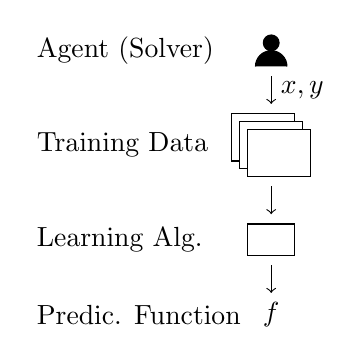
\begin{tikzpicture}
  \draw[fill=black]  (-2.8,3.7) ellipse (0.1 and 0.1);
  \draw[fill=black]  (-2.6,3.4) arc (0:180:0.2);
  \node[right] at (-5.9,3.6) {Agent (Solver)};
  \draw[fill=white]  (-3.3,2.8) rectangle (-2.5,2.2);
  \draw[fill=white]  (-3.2,2.7) rectangle (-2.4,2.1);
  \draw[fill=white]  (-3.1,2.6) rectangle (-2.3,2);
  \node[right] at (-5.9,2.4) {Training Data};
  \node (v1) at (-2.8,3.4) {};
  \node (v2) at (-2.8,2.8) {};
  \draw[->]  (v1) edge (v2);
  \node[right] at (-2.8,3.1) {$x, y$};
  \node (v3) at (-2.8,2) {};
  \node (v4) at (-2.8,1.4) {};
  \draw[->]  (v3) edge (v4);
  \draw  (-3.1,1.4) rectangle (-2.5,1);
  \draw  (-2.4,3.2) rectangle (-2.4,3.2);
  \node[right] at (-5.9,1.2) {Learning Alg.};
  \node (v5) at (-2.8,1) {};
  \node (v6) at (-2.8,0.4) {};
  \draw[->]  (v5) edge (v6);
  \node[right] at (-5.9,0.25) {Predic. Function};
  \node at (-2.8,0.25) {$f$};
  \end{tikzpicture}
  }
  \caption{Passive.}
  \label{fig:passive}
  \end{subfigure}
  &
  \begin{subfigure}[b]{0.33\textwidth}
  \centering
  \resizebox{!}{2.75cm}{
  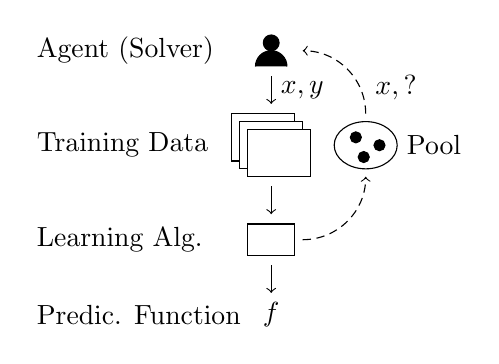
\begin{tikzpicture}
  \draw[fill=black]  (-2.8,3.7) ellipse (0.1 and 0.1);
  \draw[fill=black]  (-2.6,3.4) arc (0:180:0.2);
  \node[right] at (-5.9,3.6) {Agent (Solver)};
  \draw[fill=white]  (-3.3,2.8) rectangle (-2.5,2.2);
  \draw[fill=white]  (-3.2,2.7) rectangle (-2.4,2.1);
  \draw[fill=white]  (-3.1,2.6) rectangle (-2.3,2);
  \node[right] at (-5.9,2.4) {Training Data};
  \node (v1) at (-2.8,3.4) {};
  \node (v2) at (-2.8,2.8) {};
  \draw[->]  (v1) edge (v2);
  \node[right] at (-2.8,3.1) {$x, y$};
  \node (v3) at (-2.8,2) {};
  \node (v4) at (-2.8,1.4) {};
  \draw[->]  (v3) edge (v4);
  \draw  (-3.1,1.4) rectangle (-2.5,1);
  \draw  (-2.4,3.2) rectangle (-2.4,3.2);
  \node[right] at (-5.9,1.2) {Learning Alg.};
  \node (v5) at (-2.8,1) {};
  \node (v6) at (-2.8,0.4) {};
  \draw[->]  (v5) edge (v6);
  \node[right] at (-5.9,0.25) {Predic. Function};
  \node at (-2.8,0.25) {$f$};
  \node[right] at (-1.2,2.4) {Pool};
  \draw[->, densely dashed] (-2.4,1.2) arc (-90:0:0.8);
  \draw[->, densely dashed] (-1.6,2.8) arc (0:90:0.8);
  \node[right] at (-1.6,3.135) {$x, ?$};
  \draw  (-1.6,2.4) ellipse (0.4 and 0.3);
  \draw[fill=black]  (-1.725,2.5) ellipse (0.07 and 0.07);
  \draw[fill=black]  (-1.625,2.25) ellipse (0.07 and 0.07);
  \draw[fill=black]  (-1.425,2.4) ellipse (0.07 and 0.07);
  \end{tikzpicture}
  }
  \caption{Active Pool-based.}
  \label{fig:activepool}
  \end{subfigure}
  &
  \begin{subfigure}[b]{0.33\textwidth}
  \centering
  \resizebox{!}{2.75cm}{
  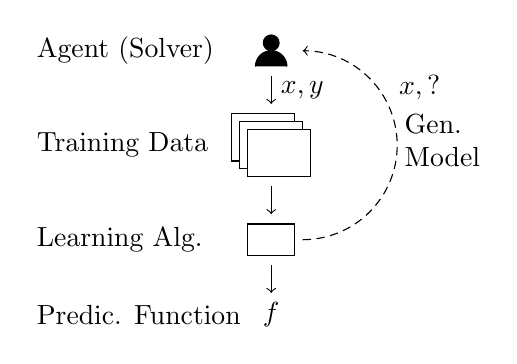
\begin{tikzpicture}
  \draw[fill=black]  (-2.8,3.7) ellipse (0.1 and 0.1);
  \draw[fill=black]  (-2.6,3.4) arc (0:180:0.2);
  \node[right] at (-5.9,3.6) {Agent (Solver)};
  \draw[fill=white]  (-3.3,2.8) rectangle (-2.5,2.2);
  \draw[fill=white]  (-3.2,2.7) rectangle (-2.4,2.1);
  \draw[fill=white]  (-3.1,2.6) rectangle (-2.3,2);
  \node[right] at (-5.9,2.4) {Training Data};
  \node (v1) at (-2.8,3.4) {};
  \node (v2) at (-2.8,2.8) {};
  \draw[->]  (v1) edge (v2);
  \node[right] at (-2.8,3.1) {$x, y$};
  \node (v3) at (-2.8,2) {};
  \node (v4) at (-2.8,1.4) {};
  \draw[->]  (v3) edge (v4);
  \draw  (-3.1,1.4) rectangle (-2.5,1);
  \draw  (-2.4,3.2) rectangle (-2.4,3.2);
  \node[right] at (-5.9,1.2) {Learning Alg.};
  \node (v5) at (-2.8,1) {};
  \node (v6) at (-2.8,0.4) {};
  \draw[->]  (v5) edge (v6);
  \node[right] at (-5.9,0.25) {Predic. Function};
  \node at (-2.8,0.25) {$f$};
  \node[right, label={[align=left]Gen.\\Model}] at (-0.75,1.88) {};
  \node[right] at (-1.3,3.135) {$x, ?$};
  \draw[->, densely dashed] (-2.4,1.2) arc (-90:90:1.2);
  \end{tikzpicture}
  }
  \caption{Active Synthesis-based.}
  \label{fig:activesynth}
  \end{subfigure}
  \end{tabular}
  \caption{Types of machine learning (depiction inspired by Rubens~et~al.~\cite{RubensESK15}).}
  \label{fig:learning}
\end{figure}


\section{Active Learning for SAT Solver Benchmarking}
\label{sec:main}

Algorithm~\ref{algALBenchmark} outlines our benchmarking framework. 
Given a set of solvers~$\mathcal{A}$, instances~$\mathcal{I}$, and runtimes~$r$, we first initialize a prediction model~$\mathcal{M}$ for the new solver $\hat a \not\in \mathcal{A}$ (Line~1).
The prediction model~$\mathcal{M}$ is used to select instances repeatedly (Line~4) for benchmarking the new solver $\hat a$ (Line~5). 
The acquired result is subsequently employed to update the prediction model (Line~7). 
When the stopping criterion is met (Line~3), the benchmarking loop terminates, and the final score of $\hat{a}$ is estimated (Line~8). 
Algorithm~\ref{algALBenchmark} returns this score, along with the acquired benchmark instances and runtime measurements. 

Section~\ref{sec:main:model} describes the underlying prediction model~$\mathcal{M}$ and outlines the methodology for deriving a solver ranking from it.
Section~\ref{sec:main:selection} presents the criteria for selecting instances.
Finally, Section~\ref{sec:main:stopping} presents potential stopping conditions.

\begin{algorithm}[t]
  \caption{Incremental Benchmarking Framework}
  \label{algALBenchmark}

  \KwIn{Solvers $\mathcal{A}$, Instances $\mathcal{I}$, Runtimes $r : \mathcal{A} \times \mathcal{I} \rightarrow [0, \tau]$, Solver $\hat{a}$}
  \KwOut{Predicted Score of $\hat{a}$, Measured Runtimes $\mathcal{R}$}

  \BlankLine

  $\mathcal{M} \leftarrow \operatorname{initModel}\left(\mathcal{A},\, \mathcal{I},\, r\right)$ \tcp*{cf. Section~\ref{sec:main:model}}
  
  \BlankLine
  $\mathcal{R} \leftarrow \emptyset$ \;
  \While(\tcp*[f]{cf. Section~\ref{sec:main:stopping}}){$\operatorname{not} \operatorname{stop}\left(\mathcal{M}\right)$}{
    $e \leftarrow \operatorname{selectNextInstance}\left(\mathcal{M}\right)$ \tcp*{cf. Section~\ref{sec:main:selection}}

    $t \leftarrow \operatorname{runExperiment}\left(\hat{a},\,  e\right)$  \tcp*{Runs $\hat{a}$ on $e$ with timeout $\tau$}

    $\mathcal{R} \leftarrow \mathcal{R} \cup \left\lbrace (e,\, t) \right\rbrace$

    \BlankLine
    $\operatorname{updateModel}\left(\mathcal{M},\, \mathcal{R}\right)$ \tcp*{cf. Section~\ref{sec:main:model}}
  }
  $s_{\hat a} \leftarrow \operatorname{predictScore}(\mathcal{M})$ \tcp*{cf. Section~\ref{sec:main:model}}
  
  \BlankLine
  \Return $(s_{\hat a}, \mathcal{R})$
\end{algorithm}


\subsection{Solver Model}
\label{sec:main:model}

The model $M$ provides a prediction function $f_{\hat a} : \mathcal{I} \rightarrow \mathbb{R}$ for solver $\hat a$.
This prediction function powers instance selection as described in Section~\ref{sec:main:selection}.
In the update step (Algorithm~\ref{algALBenchmark},~Line~7), the model is trained to predict a transformed version of solver runtime (cf.~Section~\ref{sec:main:model:transformation}) for the new solver~$\hat{a}$, using the features described in Section~\ref{sec:exdesign:data} and the previously acquired runtimes~$\mathcal{R}$.
Each iteration trains a new prediction model from scratch since the time for running the solver~$\hat{a}$ on one instance~$e$ (Line~5) dominates the training time of the model~$M$ on all acquired instances~$\mathcal{R}$ by a significant margin.
Once the benchmarking loop terminates, the score of the new solver~$\hat{a}$ is predicted and then returned (Lines~8--9).

\subsubsection{Runtime Transformation}
\label{sec:main:model:transformation}

For the prediction model~$M$, we transform the real-valued runtimes into discrete runtime labels on a per-instance basis.
For each instance $e \in \mathcal{I}$, we use a clustering algorithm to assign the runtimes in $\bigl\{ r(a, e) \mid a \in \mathcal{A} \bigr\}$ to one of $k$ clusters $C_1, \dots, C_k$ such that the fastest runtimes for the benchmark instance $e$ are in cluster $C_1$ and the slowest are in cluster $C_{k-1}$.
Timeouts $\tau$ always form a separate cluster $C_{k}$.
The runtime transformation function $\gamma_k : {\mathcal{A} \times \mathcal{I}} \rightarrow \left\lbrace 1, \dots, k \right\rbrace$ is then specified as follows:
%
$$\gamma_k(a, e) = j ~\Leftrightarrow~ r(a, e) \in C_j$$
%
Empirical studies on portfolio solvers have demonstrated that discretization is an effective approach in practice~\cite{CollauttiMMO13,NgokoCT19}.
Section~\ref{sec:exdesign:disc-pred} presents a detailed analysis of the runtime transformation in our scenario.
In particular, the analysis demonstrates that our benchmarking approach achieves higher ranking accuracy when working with discrete runtime labels rather than raw runtimes.

\subsubsection{Ranking Solvers}
\label{sec:main:model:ranking}

To determine the rank of solvers, we apply PAR-2 scoring to the discrete runtime labels $\gamma_k(a, e)$ and obtain the adapted scoring function $s_k : \mathcal{A} \rightarrow [1, 2 \cdot k]$:
%
\begin{align}
  s_k(a) := \frac{1}{|\mathcal{I}|} \sum_{e \in \mathcal{I}} \gamma'_k(a, e)
  &&
  \gamma'_k(a, e) := \begin{cases}
    2 \cdot \gamma_k(a, e)   & \text{if } \gamma_k(a, e) = k\\
  \gamma_k(a, e)  & \text{otherwise}
  \end{cases}
  \label{eq:rankingeq}
\end{align}
%
In particular, timeouts are still penalized.

\subsection{Instance Selection}
\label{sec:main:selection}

Selecting an instance based on the prediction model is a core functionality of our framework (cf.~Algorithm~\ref{algALBenchmark}, Line~4).
In this section, we introduce two instance sampling strategies, one that minimizes uncertainty and one that maximizes information gain.
Both strategies use the model's prediction function~$f$ and are inspired by existing work on active learning~\cite{settles2009active}.
These methods require the model's predictions to include probabilities for the $k$ discrete runtime labels.
Let $f_{\hat a}' : \mathcal{I} \rightarrow \left[0, 1\right]^k$ denote this modified prediction function.
In the following, the set $\tilde{\mathcal{I}} \subseteq \mathcal{I}$ denotes the instances that have already been sampled.

\paragraph{Uncertainty Sampling}

The uncertainty sampling strategy selects the instance closest to the model's decision boundary.
This is achieved by selecting the instance $e \in \mathcal{I} \setminus \tilde{\mathcal{I}}$ that minimizes the certainty~$U(e)$, which is specified by the following equation:
%
\begin{equation*}
  \operatorname{U}(e) := \left\lvert \frac{1}{k} - \max_{n \in \left\lbrace 1, \dots, k \right\rbrace} f_{\hat{a}}'(e)_{n} \right\rvert
\end{equation*}

\paragraph{Information-Gain Sampling}

The information-gain sampling strategy selects the instance with the highest expected entropy reduction regarding the runtime labels.
To be more precise, we select the instance $e \in \mathcal{I} \setminus \tilde{\mathcal{I}}$ that maximizes $IG(e)$, which is specified in the following equation:
%
\begin{equation*}
  \operatorname{IG}(e) := \operatorname{H}(e) - \sum_{n = 1}^{k} f_{\hat{a}}'(e)_{n} \operatorname{\hat H}(e)_n
\end{equation*}
%
In the equation, $\operatorname{H}(e)$ denotes the entropy of the runtime labels $\gamma(a, e)$ over all $a \in \mathcal{A}$ and $\operatorname{\hat H}(e)$ denotes the entropy of these labels plus the runtime label for $\hat{a}$.
The term $\operatorname{\hat H}(e)_n$ is computed for every possible runtime label $n \in \{1, \dots, k\}$.
By maximizing the information gain, instances are selected that identify solvers with similar runtime cluster labels, i.e., the new solver ranks similarly to the solvers in the same clusters.

\subsection{Stopping Criteria}
\label{sec:main:stopping}

In this section, we present the two dynamic stopping criteria (cf.~Algorithm~\ref{algALBenchmark}, Line~3) employed in our experiments: the Wilcoxon and the ranking stopping criterion.

\paragraph{Wilcoxon Stopping Criterion}

The Wilcoxon stopping criterion terminates the active-learning process based on the confidence that the predicted runtime labels of the new solver are sufficiently different from those of existing solvers.
This criterion is loosely inspired by Matricon et~al.~\cite{MatriconAFSH21}.
To assess the statistical significance of the predicted runtime labels, the criterion uses the average $p$-value $W_{\hat{a}}$ of a Wilcoxon signed-rank test $\operatorname{w}(S,P)$ of the runtime label distributions ${S=\{ \gamma(a, e) \mid e \in \mathcal{I} \}}$ for an existing solver $a$ and \mbox{$P=\{ f_{\hat a}(e) \mid e \in \mathcal{I} \}$} of the new solver $\hat{a}$:
%
\begin{equation*}
  W_{\hat{a}} := \frac{1}{\lvert \mathcal{A} \rvert} \sum_{a \in \mathcal{A}} \operatorname{w}(S, P)
\end{equation*}
%
To improve the stability of this criterion and mitigate the impact of outliers, we employ an exponential moving average~$W^{(i)}_{\exp}$:
%
\begin{align*}
  W_{\exp}^{\left(0\right)} &:= 1\\
  W_{\exp}^{\left(i\right)} &:= \beta W_{\hat{a}} + \left(1 - \beta\right) W_{\exp}^{\left(i - 1\right)}
\end{align*}
%
Active learning terminates when the value of $W^{(i)}_{\exp}$ drops below a fixed threshold.

\paragraph{Ranking Stopping Criterion}

In contrast, the ranking stopping criterion is less sophisticated than the previous one.
In this case, active learning terminates when the ranking induced by the model's predictions (cf.~Equation~\eqref{eq:rankingeq}) has remained unchanged within the last~$l$~iterations.
While the concrete values of the predicted score $s_{\hat a}$ may still change, the induced ranking is of sole interest in this criterion.

\section{Experimental Design}
\label{sec:exdesign}

This section outlines the experimental design employed in the presented study.
This includes an overview of the evaluation framework (cf.~Section~\ref{sec:exdesign:eval}), the datasets employed (cf.~Section~\ref{sec:exdesign:data}), the hyperparameter configuration (cf.~Section~\ref{sec:exdesign:hyper}), the runtime discretization (cf.~Section~\ref{sec:exdesign:disc-pred}), and the implementation (cf.~Section~\ref{sec:exdesign:impl}).

\subsection{Evaluation Framework}
\label{sec:exdesign:eval}

\begin{algorithm}[tb]
  \caption{Evaluation Framework}
  \label{alg:eval}

  \KwIn{Solvers $\mathcal{A}$, Instances $\mathcal{I}$, Runtimes $r : \mathcal{A} \times \mathcal{I} \rightarrow [0, \tau]$}
  \KwOut{Average Ranking Accuracy $\bar{O}_{\operatorname{acc}}$, Average Fraction of Runtime $\bar{O}_{\operatorname{rt}}$}
  \BlankLine

  $O \leftarrow \emptyset$
  % \BlankLine

  \For{$\hat{a} \in \mathcal{A}$}{
    $\mathcal{A}' \leftarrow \mathcal{A} \setminus \left\lbrace \hat{a} \right\rbrace$ \;
    $(s_{\hat a}, \mathcal{R}) \leftarrow \operatorname{runALAlgorithm}(\mathcal{A}', \mathcal{I}, r, \hat{a})$ \tcp*{Refer to Algorithm~\ref{algALBenchmark}}

  \BlankLine
  \tcp{Determine Ranking Accuracy}
    $O_{\operatorname{acc}} \leftarrow 0$ \;    
    \For{$a \in \mathcal{A}'$}{
      \If{$\bigl(s_k(a) - s_{\hat a}\bigr) \cdot \bigl(\operatorname{par_2}(a) - \operatorname{par_2}(\hat a)\bigr) > 0$}{
           $O_{\operatorname{acc}} \leftarrow O_{\operatorname{acc}} + \frac{1}{|\mathcal{A}'|}$ \;
      }
    }
  
  \BlankLine
  \tcp{Determine Runtime Fraction}
  $t_{\text{total}} \leftarrow \sum\limits_{e \in \mathcal{I}} r(\hat a, e)$\;
  $O_{\operatorname{rt}} \leftarrow 0$\;
    \For{$e \in \mathcal{I}$}{
    \If{$\exists t, (e,t) \in \mathcal{R}$}{
      $O_{\operatorname{rt}} \leftarrow O_{\operatorname{rt}} + \frac{t}{t_{\text{total}}}$\;
    }
  }
  
  % \BlankLine
    $O \leftarrow O \cup \bigl\{ ( O_{\operatorname{acc}},\, O_{\operatorname{rt}} ) \bigr\}$
  }

  % \BlankLine
  $\bigl( \bar{O}_{\operatorname{acc}}, \bar{O}_{\operatorname{rt}} \bigr) \leftarrow \operatorname{average}(O)$ \;
  
  % \BlankLine
  \Return $\bigl( \bar{O}_{\operatorname{acc}}, \bar{O}_{\operatorname{rt}} \bigr)$
\end{algorithm}

To assess our active-learning framework, we perform cross-validation over a set of solvers (cf.~Algorithm~\ref{alg:eval}).
Each solver assumes the role of the new solver~$\hat{a}$ once (Line~2) and is therefore excluded from the set of solvers $\mathcal{A}$ in that iteration (Line~3).
After running active learning for solver~$\hat{a}$ (Line~4), we compute the value of two optimization goals, i.e., ranking accuracy and runtime.
The \emph{ranking accuracy} $O_{\operatorname{acc}} \in \left[0, 1\right]$ (higher is better) is defined as the fraction of correctly ranked solver pairs~$\left(\hat{a}, a\right)$ regarding the PAR-2 scoring, where $a$ belongs to the set of all solvers $\mathcal{A}$ (Lines~5--8).
The \emph{fraction of runtime} required by the framework to reach its conclusion is represented by $O_{\operatorname{rt}} \in [0, 1]$ (lower is better).
This metric compares the accumulated runtimes over the sampled instances to the accumulated runtimes over all instances in the dataset (Lines~9--13).
Once all cross-validation results have been collected (Line~14), the output metrics are averaged and returned (Lines~15--16).

To compare different instantiations of our active-learning framework holistically, we insert the cross-validation results into Equation~\eqref{eq:opt}:
%
\begin{equation}
	O_\delta := \delta O_{\operatorname{acc}} + \left(1 - \delta\right) \left(1 - O_{\operatorname{rt}}\right) \enspace \textrm{,}
	\label{eq:opt}
\end{equation} 
%
$\delta \in \left[0, 1\right]$ is a factor for weighting the two optimization goals $O_{\operatorname{acc}}$ and $O_{\operatorname{rt}}$.
Plotting the approaches that maximize $O_\delta$ for all $\delta \in \left[0, 1\right]$ on an $O_{\operatorname{rt}}$-$O_{\operatorname{acc}}$-diagram provides us with a Pareto front of the best approaches for different optimization-goal weightings.

\subsection{Data}
\label{sec:exdesign:data}

In our experiments, we work with the dataset of the SAT~Competition~2022 Anniversary Track~\cite{sat2022,zenodoanniversarytrack}.
This dataset consists of 5355 instances with corresponding runtimes of 28 sequential SAT solvers.
For predictions within our framework, we also use a database of 56 instance features\footnote{\url{https://benchmark-database.de/getdatabase/base_db}} from the Global Benchmark Database~(GBD)~\cite{GBD24paper}.
They include instance size features and node distribution statistics for several graph representations of SAT instances, and are primarily inspired by the SATzilla~2012 features described in~\cite{features}.
All features are numeric and have no missing values.
We drop 10 of the 56 features due to zero variance.
In total, the prediction models have access to 46 instance features and 27 out of 28 runtime features, excluding the respective new solver~$\hat{a}$.

In addition, we retrieve instance family information\footnote{\url{https://benchmark-database.de/getdatabase/meta_db}} to evaluate the composition of our sampled benchmarks.
Instance families consist of instances from the same application domain, such as planning, cryptography, etc., and are valuable for analyzing solver performance.
%
For hyperparameter tuning, we randomly sample \SI{10}{\%} of the complete set of 5355 instances with stratification regarding the instance family.
All instance families that are too \emph{small}, i.e., families with less than 10 instances, are put into one meta-family for stratification.
This \emph{tuning dataset} allows a more extensive exploration of the hyperparameter space.

\subsection{Hyperparameters}
\label{sec:exdesign:hyper}

There are several possible instantiations for the three subroutines \emph{ranking}, \emph{selection}, and \emph{stopping} in Algorithm~\ref{algALBenchmark}.
We describe these experimental configurations next.

\subparagraph{Ranking}

Regarding \emph{ranking} (cf.~Section~\ref{sec:main:model}), we experiment with the following instantiations:

\begin{itemize}\setlength{\itemsep}{1pt}
  \item Observed PAR-2 ranking of already sampled instances, without using prediction
  \item Predicted runtime-label ranking
  \vspace*{-1ex}
  \begin{itemize}\setlength{\itemsep}{1pt}
    \item
    History size: For stability, consider the latest 1, 10, 20, 30, or 40 predictions within a voting approach.
    The latest $x$ predictions for each instance vote on the instance's winning label.
    \item
    Fallback threshold: If the difference of scores between the new solver~$\hat{a}$ and another solver drops below \SI{0.01}, \SI{0.05}, or \SI{0.1}, use the partially observed PAR-2 ranking as a tie-breaker.
  \end{itemize}
\end{itemize}

\subparagraph{Selection}

We experiment with the following instantiations of the instance \emph{selection} (cf. Section~\ref{sec:main:selection}).
Since the potential runtime of the solver experiments is orders of magnitude larger than the model update time, we increment our benchmark one instance at a time rather than using batches of multiple instances.
Both are used in the state-of-the-art in active learning~\cite{SinhaED19,2019gaal}.
A drawback of this is the lack of parallel execution of runtime experiments.

\begin{itemize}\setlength{\itemsep}{1pt}
  \item Random sampling 
  \item Uncertainty sampling
  \vspace*{-1ex}
  \begin{itemize}\setlength{\itemsep}{1pt}
    \item Fallback threshold: Use random sampling for the first \SI{0}{\%}, \SI{5}{\%}, \SI{10}{\%}, \SI{15}{\%}, or \SI{20}{\%} of instances to explore the instance space.
    \item Runtime scaling: Whether to scale the uncertainty scores by the average runtime of solvers or use $\operatorname{U}(e)$ as is.
  \end{itemize}

  \item Information-gain sampling
  \vspace*{-1ex}
  \begin{itemize}
    \item Fallback threshold: Use random sampling for the first \SI{0}{\%}, \SI{5}{\%}, \SI{10}{\%}, \SI{15}{\%}, or \SI{20}{\%} of instances to explore the instance space.
    \item Runtime scaling: Whether to normalize information-gain scores per instance by the average runtime of solvers on it or use the absolute values.
  \end{itemize}
\end{itemize}

\subparagraph{Stopping}

We evaluate the following \emph{stopping} (cf. Section~\ref{sec:main:stopping}) criteria:

\begin{itemize}\setlength{\itemsep}{1pt}
  \item Subset-size stopping criterion: Stop after sampling \SI{10}{\%} or \SI{20}{\%} of instances.
  \item Ranking stopping criterion
  \vspace*{-1ex}
  \begin{itemize}\setlength{\itemsep}{1pt}
    \item Minimum amount: Sample at least \SI{2}{\%}, \SI{8}{\%}, \SI{10}{\%}, or \SI{12}{\%} of instances before applying the criterion.
    \item Convergence duration: Stop if the predicted ranking stays the same for a number of sampled instances equal to \SI{1}{\%} or \SI{2}{\%} of all instances.
  \end{itemize}
  \item Wilcoxon stopping criterion
  \vspace*{-1ex}
  \begin{itemize}\setlength{\itemsep}{1pt}
    \item Minimum amount: Sample at least \SI{2}{\%}, \SI{8}{\%}, \SI{10}{\%}, or \SI{12}{\%} of instances before applying the criterion.
    \item Average of $p$-values to drop below: \SI{5}{\%}.
    \item Exponential moving average: Incorporate previous significance values by using an EMA with $\beta = 0.1$ or $\beta = 0.7$.
  \end{itemize}
\end{itemize}

\subsection{Runtime Discretization and Prediction}
\label{sec:exdesign:disc-pred}

One of the most important parts of our framework is the solver runtime model (cf.~Section~\ref{sec:main:model}).
In this section, we detail how clustering solver runtimes can lead to informative runtime labels and which machine learning models are best at predicting them.
To this end, we analyze prediction performance for estimating runtimes, timeouts, and discretized runtimes.

\paragraph{Regressing Runtime}

\begin{table}[tb]
	\centering
	\caption{Test-set prediction performance for predicting solver runtime (a continuous target) with two prediction models.}
	\label{tab:regression}
	\begin{tabular}{lcc}
		\toprule
		{Regression Models} & {Avg. RMSE ($\pm$ std)} & {Avg. MAE ($\pm$ std)} \\
		\midrule
		Random Forest & \SI{1929.84}{s} ($\pm$ \SI{1161.15}{s}) & \phantom{0}\SI{957.36}{s} ($\pm$ \SI{297.21}{s}) \\[0.4ex]
		Multilayer Perceptron & \SI{2275.20}{s} ($\pm$ \SI{1545.01}{s}) & \SI{1284.30}{s} ($\pm$ \SI{390.57}{s}) \\
		\bottomrule
	\end{tabular}
\end{table}

As a baseline, Table~\ref{tab:regression} shows the prediction performance of two regression models, i.e., a random forest and a multilayer perceptron.
We employ these models to estimate a new solver's raw runtime as the prediction target.
To this end, we use 46 instance features and 27 known solver runtimes as inputs for the predictions.
We repeat this evaluation for each solver as the prediction target and report the average and standard deviation of prediction performance over the 28 solvers.

We chose both types of prediction models for their robustness and ability to capture nonlinear dependencies~\cite{breiman2001random}.
However, both still perform poorly, as evidenced by the magnitudes of the mean regression errors in Table~\ref{tab:regression}.
In particular, a root mean squared error (RMSE) of about \SI{2000}{s} is relatively high for solver runtimes that range from 0 to \SI{5000}{s}.
Such unreliable runtime estimates could affect active learning negatively.
Therefore, we decided to discretize the runtimes for prediction, moving from a regression scenario to a classification scenario.

\paragraph{Classifying Timeouts}

\begin{table}[tb]
	\centering
	\caption{Test-set prediction performance for predicting solver timeouts (a binary target) with different prediction models.}
	\label{tab:timeout-prediction}
	~\\[1em]
	\begin{tabular}{lcc}
		\toprule
		\multirow[c]{2}{*}{Timeout Prediction Models} & \multicolumn{2}{c}{Average MCC ($\pm$ std)} \\
		\cmidrule(lr){2-3}
		& {Without Runtime Feat.} & {With Runtime Feat.} \\
		\midrule
		Stacking (QDA\,+\,RF)                 & 0.6513 ($\pm$ 0.0458) & 0.9527 ($\pm$ 0.0292) \\[0.4ex]
		Quadratic Discriminant Analysis (QDA)                    & 0.2593 ($\pm$ 0.1310) & 0.9290 ($\pm$ 0.0339) \\[0.4ex]
		Random Forest (RF)         & 0.6607 ($\pm$ 0.0547) & 0.8530 ($\pm$ 0.0479) \\[0.4ex]
		AdaBoost                             & 0.5412 ($\pm$ 0.0612) & 0.8384 ($\pm$ 0.0444) \\[0.4ex]
		Decision Tree                         & 0.5980 ($\pm$ 0.0423) & 0.8059 ($\pm$ 0.0707) \\[0.4ex]
		Logistic Regression                   & 0.2031 ($\pm$ 0.0728) & 0.8052 ($\pm$ 0.1018) \\[0.4ex]
		$k$NN                   & 0.5108 ($\pm$ 0.0387) & 0.7885 ($\pm$ 0.1521) \\[0.4ex]
		Multilayer Perceptron                      & 0.1293 ($\pm$ 0.0718) & 0.7760 ($\pm$ 0.1408) \\[0.4ex]
		Support Vector Machine               & 0.0595 ($\pm$ 0.0554) & 0.7757 ($\pm$ 0.2149) \\[0.4ex]
		Naive Bayes                           & 0.1173 ($\pm$ 0.0872) & 0.7306 ($\pm$ 0.1394) \\
		\bottomrule
	\end{tabular}
\end{table}

Table~\ref{tab:timeout-prediction} shows the prediction performance for estimating whether a solver times out or not.
This binary prediction target represents a very strong discretization of runtimes.
We compare a variety of prediction models that pursue different learning paradigms.
Each is trained with either instance features only (second column) or instance and runtime features (third column).
As the evaluation metric for prediction performance, we use Matthews Correlation Coefficient (MCC)~\cite{gorodkin2004comparing, matthews1975comparison}, which reaches its maximum of~1 for a perfect prediction, is~0 for random guessing, and has a minimum of~-1.

Training the classification models with instance features only, a random forest performs best.
In contrast, a quadratic discriminant analysis performs poorly in this scenario but performs very well if runtime features are included.
However, the best prediction performance with all features is achieved by a stacking ensemble~\cite{wolpert1992stacked} out of the quadratic discriminant analysis~\cite{tharwat2016linear} and the random forest~\cite{breiman2001random}.
Stacking means that another model, in our case a simple decision tree~\cite{breiman1984classification}, makes a prediction based on the predictions of the ensembled models.

\paragraph{Classifying Discretized Runtime Labels}

Building on the success of binary timeout prediction, we investigate a classification scenario where the target is solver runtime discretized into multiple categories.

\subparagraph{Label definition}

To define this prediction target, we partition the solver runtimes into $k$~clusters.
We conduct this clustering step per instance, i.e., the solvers forming a particular cluster may differ from instance to instance.
The adapted solver scoring function~$s_k$ (cf.~Equation~\eqref{eq:rankingeq}) subsequently uses the cluster labels.
In preliminary experiments, the most \emph{useful} labels were produced with hierarchical clustering and a log-single-linkage criterion; we will discuss our notion of label usefulness later.
Other clustering approaches we have tried include hierarchical clustering with mean-, median-, and complete-linkage criteria, as well as $k$-means and spectral clustering.

In our chosen hierarchical clustering procedure, each non-timeout runtime starts in a separate cluster.
We then gradually merge the closest clusters until the desired number of $k-1$ partitions is reached.
By definition, the $k$-th cluster always contains the timeouts and no other runtimes (cf.~Section~\ref{sec:main:model:transformation}).
To quantify the distance between two clusters, we consider the minimum pairwise difference of logarithmic runtimes between solvers from the two clusters.

\subparagraph{Label prediction}

\begin{table}[tb]
  \centering
  \caption{Test-set prediction performance for predicting the $C_k$ cluster labels (a discrete target) with the best-performing models.}
  \label{tab:cluster-prediction}
  \begin{tabular}{lcc}
    \toprule
    \multirow[c]{2}{*}{$C_3$ Cluster Prediction Models} & \multicolumn{2}{c}{Average MCC ($\pm$ std)} \\
    \cmidrule(lr){2-3}
    & {Without Clustering Feat.} & {With Clustering Feat.} \\
    \midrule
    Stacking (QDA\,+\,RF)                 & 0.7464 ($\pm$ 0.0497) & 0.8380 ($\pm$ 0.0634) \\[0.4ex]
    Quadratic Discriminant Analysis (QDA)                     & 0.6903 ($\pm$ 0.0607) & 0.7738 ($\pm$ 0.0459) \\[0.4ex]
    Random Forest (RF)         & 0.7116 ($\pm$ 0.0385) & 0.7841 ($\pm$ 0.0469) \\[0.4ex]
    \midrule
    \multirow[c]{2}{*}{$C_4$ Cluster Prediction Models} & \multicolumn{2}{c}{Average MCC ($\pm$ std)} \\
    \cmidrule(lr){2-3}
    & {Without Clustering Feat.} & {With Clustering Feat.} \\
    \midrule
    Stacking (QDA\,+\,RF)                 & 0.6562 ($\pm$ 0.0538) & 0.7366 ($\pm$ 0.0377) \\[0.4ex]
    Quadratic Discriminant Analysis (QDA)                     & 0.6007 ($\pm$ 0.0765) & 0.6872 ($\pm$ 0.0469) \\[0.4ex]
    Random Forest (RF)         & 0.6033 ($\pm$ 0.0455) & 0.6828 ($\pm$ 0.0527) \\[0.4ex]
    \midrule
    \multirow[c]{2}{*}{$C_5$ Cluster Prediction Models} & \multicolumn{2}{c}{Average MCC ($\pm$ std)} \\
    \cmidrule(lr){2-3}
    & {Without Clustering Feat.} & {With Clustering Feat.} \\
    \midrule
    Stacking (QDA\,+\,RF)                 & 0.5835 ($\pm$ 0.0615) & 0.6396 ($\pm$ 0.0553) \\[0.4ex]
    Quadratic Discriminant Analysis (QDA)                      & 0.5508 ($\pm$ 0.0669) & 0.5881 ($\pm$ 0.0912) \\[0.4ex]
    Random Forest (RF)         & 0.5420 ($\pm$ 0.0459) & 0.5895 ($\pm$ 0.0475) \\
    \bottomrule
  \end{tabular}
\end{table}

Next, we use the runtimes labels from this discretization procedure as prediction targets.
Table~\ref{tab:cluster-prediction} shows the prediction performance for the best classification models from Table~\ref{tab:timeout-prediction} and $k \in \lbrace 3, 4, 5 \rbrace$ clusters.
We train the prediction models either with 46 instance features and 27 known solver runtimes (second column) or additionally including 27 features representing the known $C_k$ cluster labels of other solvers (third column).

For all prediction models and values of~$k$, the prediction performance is better when the cluster labels are included as features.
In addition, the prediction performance degrades rapidly as the number of clusters increases.
The stacking ensemble performs best in all cases, so we use it in all subsequent experiments.

\begin{figure}[tb]
	\centering
	\begin{subfigure}{0.45\textwidth}
		\centering
		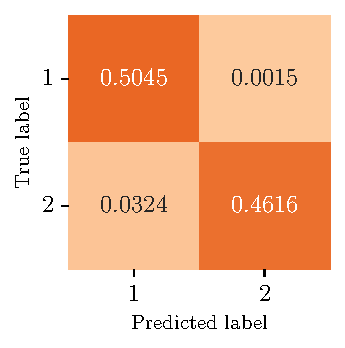
\includegraphics[height=4.123cm]{plots/cm2labels.pdf}
		\caption{Timeout prediction.}
	\end{subfigure}
	\begin{subfigure}{0.45\textwidth}
		\centering
		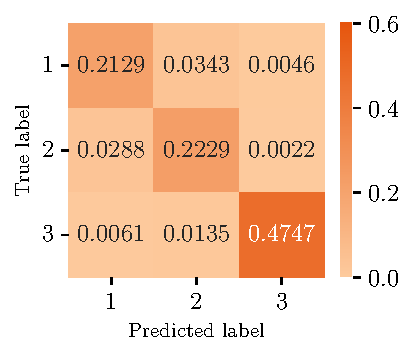
\includegraphics[height=4.228cm]{plots/cm3labels.pdf}
		\caption{$C_3$ cluster prediction.}
	\end{subfigure}
	\caption{Confusion matrices for predicting timeouts and $C_3$ cluster labels.}
	\label{fig:confusion-matrices}
\end{figure}

To analyze the stacking ensemble in more depth, Fig.~\ref{fig:confusion-matrices} shows the confusion matrices for predicting timeouts and $C_3$ cluster labels.
Both scenarios admit relatively good prediction performance, with the model for $C_3$ performing slightly worse than the model for timeouts.
Notably, for $C_3$, there is less confusion between the non-timeout labels (Labels~1 and~2) and the timeout label (Label~3) than between the non-timeout labels (Labels~1 and~2).
This observation suggests that deciding on timeouts is easier than distinguishing between discretized non-timeout runtimes.

\subparagraph{Label usefulness}

% TODO tf: Actual rankings with discretization
% * Correct ranking pairs in table below: 97.45%
% * Max. difference between wrong pairs 0.11
% * Spearman correlation of PAR2 and Discrete rank: 0.9862
\begin{table}[tb]
	\centering
	\caption{Ranking of solvers for the PAR-2 score and our discretized $s_3$ score.}
	\label{tab:ranking}
	~\\[1em]
	\begin{tabular}{
			>{\centering\arraybackslash}m{0.09\textwidth}
			>{\centering\arraybackslash}m{0.15\textwidth}
			>{\centering\arraybackslash}m{0.09\textwidth}
			>{\centering\arraybackslash}m{0.15\textwidth}
			>{\raggedright\arraybackslash}m{0.01\textwidth}
			>{\raggedright\arraybackslash}m{0.314\textwidth}
		}
		\toprule
		\multicolumn{2}{c}{PAR-2} & \multicolumn{2}{c}{$s_3$} & & \multirow[c]{2}{*}{\vspace{-0.15cm}\hspace{-0.02cm}Solver} \\
		\cmidrule(r){1-2}\cmidrule(r){3-4}
		Rank &   Score & Rank &  Score & & \\
		\midrule
		1 & 2808.13 &    1 & 1.1717 & & kissat-mab-esa \\
		2 & 2812.93 &    2 & 1.1832 & & kissat-sc2022-bulky \\
		3 & 2835.25 &    3 & 1.1862 & & ekissat-mab-gb-db \\
		4 & 2835.59 &    4 & 1.1868 & & kissat-mab-ucb \\
		5 & 2836.92 &    5 & 1.1868 & & kissat-inc \\
		6 & 2845.19 &    6 & 1.1926 & & ekissat-mab-db-v1 \\
		7 & 2846.73 &    7 & 1.1930 & & kissat-mab-moss \\
		8 & 2857.67 &    8 & 1.1947 & & kissat-mab-hywalk \\
		9 & 2869.45 &    9 & 1.1998 & & kissat-sc2022-light \\
		10 & 2899.70 &   10 & 1.2164 & & kissat-els-v2 \\
		11 & 2953.59 &   11 & 1.2290 & & hkis-unsat \\
		12 & 2967.53 &   12 & 1.2347 & & kissat-adaptive-restart \\
		13 & 2976.56 &   13 & 1.2475 & & seqfrost-noextend \\
		14 & 3014.40 &   16 & 1.2645 & & kissat-els-v1 \\
		15 & 3017.73 &   14 & 1.2509 & & cadical-esa \\
		16 & 3036.83 &   15 & 1.2613 & & cadical-reorder \\
		17 & 3049.90 &   20 & 1.3648 & & cadical-rel-scavel \\
		18 & 3080.66 &   19 & 1.2965 & & kissat-relaxed \\
		19 & 3095.73 &   17 & 1.2815 & & cadical-dvdl-v1 \\
		20 & 3101.12 &   18 & 1.2856 & & cadical-dvdl-v2 \\
		21 & 3273.95 &   21 & 1.3786 & & glucose-reboot \\
		22 & 3290.90 &   25 & 1.4707 & & lstech-maple-hywalk \\
		23 & 3292.68 &   23 & 1.4478 & & lstech-maple \\
		24 & 3400.72 &   24 & 1.4693 & & slime-sc-2022-beta \\
		25 & 3412.11 &   26 & 1.5237 & & slime-sc-2022 \\
		26 & 3436.07 &   22 & 1.4161 & & hcad-v1-psids \\
		27 & 3506.32 &   27 & 1.5433 & & maple-lcmdistchrbt-dl-v3 \\
		28 & 4741.50 &   28 & 2.0581 & & isasat \\
		\bottomrule
	\end{tabular}
\end{table}

To ensure that the runtime labels also are \emph{useful} for active learning, we evaluate whether the labels still discriminate solvers and agree with the actual PAR-2 ranking.
Table~\ref{tab:ranking} shows the ranking of the solvers in the SAT Competition~2022 Anniversary Track~\cite{sat2022} according to the standard PAR-2 score and according to our discretized $s_3$ score.
We observe that ranking with our score correctly decides for almost all (about \SI{97.45}{\%}; $\sigma = \SI{3.68}{\%}$) solver pairs which solver is faster.
In particular, the Spearman correlation of $s_3$ and the PAR-2 score over all solvers is about \SI{0.988}{}, which is very close to the optimal value of~1~\cite{de2016comparing}.

% Amount of significant solver pairs (Wilcoxon signed-rank, 5% alpha):
% PAR-2:   684/756 = 0.9048
% timeout: 660/756 = 0.8730
% k=3:     662/756 = 0.8757
% k=4:     662/756 = 0.8757
% k=5:     662/756 = 0.8757
\begin{figure}[tb]
	\centering
	\begin{subfigure}{0.32\textwidth}
		\centering
		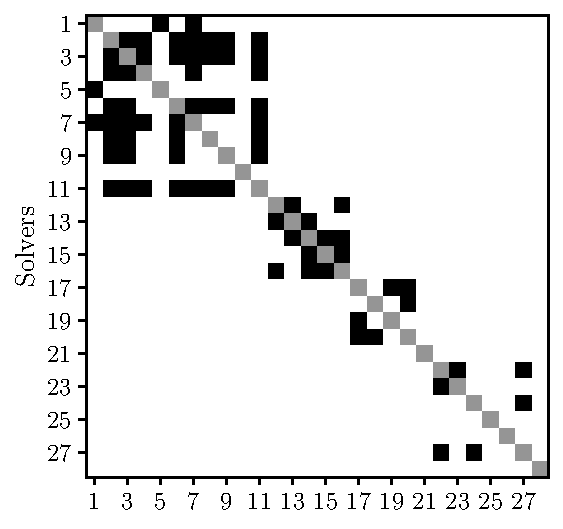
\includegraphics[width=3.9cm]{plots/par2sigdiff.pdf}
		\caption{PAR-2 scores.}
	\end{subfigure}
	\begin{subfigure}{0.32\textwidth}
		\centering
		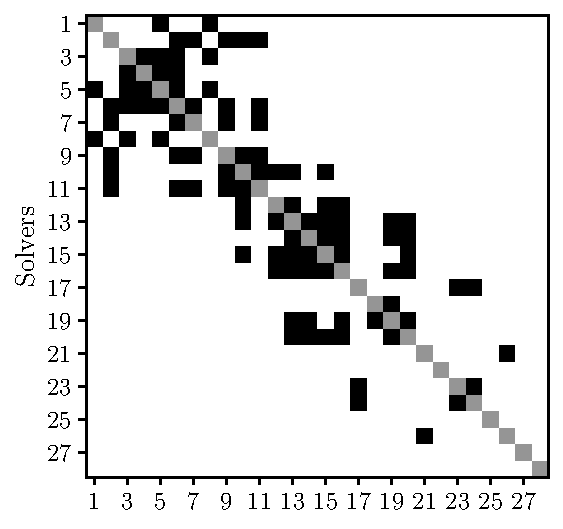
\includegraphics[width=3.9cm]{plots/timeoutsigdiff.pdf}
		\caption{Timeouts.}
	\end{subfigure}
	\begin{subfigure}{0.32\textwidth}
		\centering
		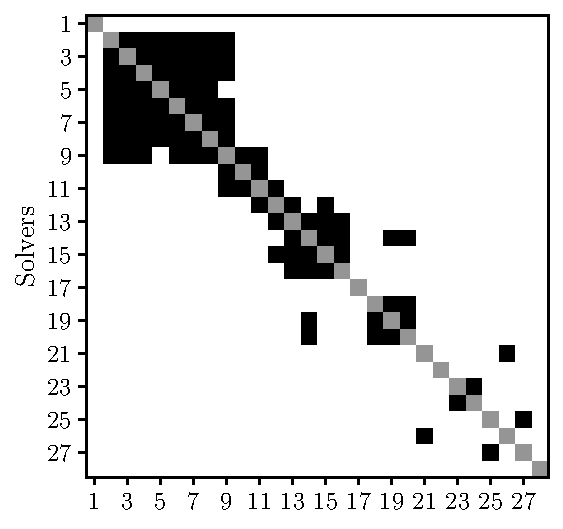
\includegraphics[width=3.9cm]{plots/s3sigdiff.pdf}
		\caption{$s_3$ scores.}
	\end{subfigure}
	\caption{Solver pairs with significant differences regarding their scorings are colored white, non-significant ones black. Solvers are ordered identically to Table~\ref{tab:ranking}.}
	\label{fig:solver-confusion-matrices}
\end{figure}

We also analyze how runtime discretization affects the distinguishability of solver pairs.
The matrices in Fig.~\ref{fig:solver-confusion-matrices} visualize which solver pairs exhibit significant differences in their PAR-2 scores, timeouts, and $s_3$ scores.
According to a Wilcoxon signed-rank test with a significance level of $\alpha = 0.05$, \SI{87.57}{\%} of the solver pairs have significantly different scores after $\gamma_3$-discretization, which is only a slight decrease compared to \SI{90.48}{\%} before discretization.
$\gamma_2$-discretization significantly distinguishes \SI{87.30}{\%} of solver pairs.
These results support the usefulness of discretized runtimes for our active learning framework.

\subsection{Implementation Details}
\label{sec:exdesign:impl}

For reproducibility, our source code and data are available on GitHub (see footnotes in Section~\ref{sec:intro}).
Our code is implemented in \textsc{Python} using \emph{scikit-learn}~\cite{scikit-learn} for making predictions, and \emph{gbd-tools}~\cite{GBD24paper} for retrieving SAT instances.


\section{Evaluation}
\label{sec:eval}

In this section, we evaluate our active learning framework.
First, we analyze and tune the different subroutines of our framework on the tuning dataset (cf.~Section~\ref{sec:eval:hyper}).
Next, we evaluate the best configurations on the full dataset (cf.~Section~\ref{sec:eval:full}).
Finally, we analyze the importance of instance families for our framework (cf.~Section~\ref{sec:eval:instance}).

\subsection{Hyperparameter Analysis}
\label{sec:eval:hyper}

\begin{figure}[tbp!]
  \centering
  \begin{subfigure}{1.0\textwidth}
    \resizebox{\textwidth}{!}{
      \graphicspath{{plots/}}
      %% Creator: Matplotlib, PGF backend
%%
%% To include the figure in your LaTeX document, write
%%   \input{<filename>.pgf}
%%
%% Make sure the required packages are loaded in your preamble
%%   \usepackage{pgf}
%%
%% Also ensure that all the required font packages are loaded; for instance,
%% the lmodern package is sometimes necessary when using math font.
%%   \usepackage{lmodern}
%%
%% Figures using additional raster images can only be included by \input if
%% they are in the same directory as the main LaTeX file. For loading figures
%% from other directories you can use the `import` package
%%   \usepackage{import}
%%
%% and then include the figures with
%%   \import{<path to file>}{<filename>.pgf}
%%
%% Matplotlib used the following preamble
%%
\begingroup%
\makeatletter%
\begin{pgfpicture}%
\pgfpathrectangle{\pgfpointorigin}{\pgfqpoint{9.333576in}{3.346586in}}%
\pgfusepath{use as bounding box, clip}%
\begin{pgfscope}%
\pgfsetbuttcap%
\pgfsetmiterjoin%
\pgfsetlinewidth{0.000000pt}%
\definecolor{currentstroke}{rgb}{1.000000,1.000000,1.000000}%
\pgfsetstrokecolor{currentstroke}%
\pgfsetstrokeopacity{0.000000}%
\pgfsetdash{}{0pt}%
\pgfpathmoveto{\pgfqpoint{-0.000000in}{0.000000in}}%
\pgfpathlineto{\pgfqpoint{9.333576in}{0.000000in}}%
\pgfpathlineto{\pgfqpoint{9.333576in}{3.346586in}}%
\pgfpathlineto{\pgfqpoint{-0.000000in}{3.346586in}}%
\pgfpathlineto{\pgfqpoint{-0.000000in}{0.000000in}}%
\pgfpathclose%
\pgfusepath{}%
\end{pgfscope}%
\begin{pgfscope}%
\pgfsetbuttcap%
\pgfsetmiterjoin%
\definecolor{currentfill}{rgb}{1.000000,1.000000,1.000000}%
\pgfsetfillcolor{currentfill}%
\pgfsetlinewidth{0.000000pt}%
\definecolor{currentstroke}{rgb}{0.000000,0.000000,0.000000}%
\pgfsetstrokecolor{currentstroke}%
\pgfsetstrokeopacity{0.000000}%
\pgfsetdash{}{0pt}%
\pgfpathmoveto{\pgfqpoint{0.746177in}{0.679475in}}%
\pgfpathlineto{\pgfqpoint{9.093551in}{0.679475in}}%
\pgfpathlineto{\pgfqpoint{9.093551in}{3.163253in}}%
\pgfpathlineto{\pgfqpoint{0.746177in}{3.163253in}}%
\pgfpathlineto{\pgfqpoint{0.746177in}{0.679475in}}%
\pgfpathclose%
\pgfusepath{fill}%
\end{pgfscope}%
\begin{pgfscope}%
\pgfsetbuttcap%
\pgfsetroundjoin%
\definecolor{currentfill}{rgb}{0.000000,0.000000,0.000000}%
\pgfsetfillcolor{currentfill}%
\pgfsetlinewidth{0.803000pt}%
\definecolor{currentstroke}{rgb}{0.000000,0.000000,0.000000}%
\pgfsetstrokecolor{currentstroke}%
\pgfsetdash{}{0pt}%
\pgfsys@defobject{currentmarker}{\pgfqpoint{0.000000in}{-0.048611in}}{\pgfqpoint{0.000000in}{0.000000in}}{%
\pgfpathmoveto{\pgfqpoint{0.000000in}{0.000000in}}%
\pgfpathlineto{\pgfqpoint{0.000000in}{-0.048611in}}%
\pgfusepath{stroke,fill}%
}%
\begin{pgfscope}%
\pgfsys@transformshift{0.746177in}{0.679475in}%
\pgfsys@useobject{currentmarker}{}%
\end{pgfscope}%
\end{pgfscope}%
\begin{pgfscope}%
\definecolor{textcolor}{rgb}{0.000000,0.000000,0.000000}%
\pgfsetstrokecolor{textcolor}%
\pgfsetfillcolor{textcolor}%
\pgftext[x=0.746177in,y=0.582253in,,top]{\color{textcolor}\rmfamily\fontsize{18.000000}{21.600000}\selectfont 0.0}%
\end{pgfscope}%
\begin{pgfscope}%
\pgfsetbuttcap%
\pgfsetroundjoin%
\definecolor{currentfill}{rgb}{0.000000,0.000000,0.000000}%
\pgfsetfillcolor{currentfill}%
\pgfsetlinewidth{0.803000pt}%
\definecolor{currentstroke}{rgb}{0.000000,0.000000,0.000000}%
\pgfsetstrokecolor{currentstroke}%
\pgfsetdash{}{0pt}%
\pgfsys@defobject{currentmarker}{\pgfqpoint{0.000000in}{-0.048611in}}{\pgfqpoint{0.000000in}{0.000000in}}{%
\pgfpathmoveto{\pgfqpoint{0.000000in}{0.000000in}}%
\pgfpathlineto{\pgfqpoint{0.000000in}{-0.048611in}}%
\pgfusepath{stroke,fill}%
}%
\begin{pgfscope}%
\pgfsys@transformshift{1.580914in}{0.679475in}%
\pgfsys@useobject{currentmarker}{}%
\end{pgfscope}%
\end{pgfscope}%
\begin{pgfscope}%
\definecolor{textcolor}{rgb}{0.000000,0.000000,0.000000}%
\pgfsetstrokecolor{textcolor}%
\pgfsetfillcolor{textcolor}%
\pgftext[x=1.580914in,y=0.582253in,,top]{\color{textcolor}\rmfamily\fontsize{18.000000}{21.600000}\selectfont 0.1}%
\end{pgfscope}%
\begin{pgfscope}%
\pgfsetbuttcap%
\pgfsetroundjoin%
\definecolor{currentfill}{rgb}{0.000000,0.000000,0.000000}%
\pgfsetfillcolor{currentfill}%
\pgfsetlinewidth{0.803000pt}%
\definecolor{currentstroke}{rgb}{0.000000,0.000000,0.000000}%
\pgfsetstrokecolor{currentstroke}%
\pgfsetdash{}{0pt}%
\pgfsys@defobject{currentmarker}{\pgfqpoint{0.000000in}{-0.048611in}}{\pgfqpoint{0.000000in}{0.000000in}}{%
\pgfpathmoveto{\pgfqpoint{0.000000in}{0.000000in}}%
\pgfpathlineto{\pgfqpoint{0.000000in}{-0.048611in}}%
\pgfusepath{stroke,fill}%
}%
\begin{pgfscope}%
\pgfsys@transformshift{2.415652in}{0.679475in}%
\pgfsys@useobject{currentmarker}{}%
\end{pgfscope}%
\end{pgfscope}%
\begin{pgfscope}%
\definecolor{textcolor}{rgb}{0.000000,0.000000,0.000000}%
\pgfsetstrokecolor{textcolor}%
\pgfsetfillcolor{textcolor}%
\pgftext[x=2.415652in,y=0.582253in,,top]{\color{textcolor}\rmfamily\fontsize{18.000000}{21.600000}\selectfont 0.2}%
\end{pgfscope}%
\begin{pgfscope}%
\pgfsetbuttcap%
\pgfsetroundjoin%
\definecolor{currentfill}{rgb}{0.000000,0.000000,0.000000}%
\pgfsetfillcolor{currentfill}%
\pgfsetlinewidth{0.803000pt}%
\definecolor{currentstroke}{rgb}{0.000000,0.000000,0.000000}%
\pgfsetstrokecolor{currentstroke}%
\pgfsetdash{}{0pt}%
\pgfsys@defobject{currentmarker}{\pgfqpoint{0.000000in}{-0.048611in}}{\pgfqpoint{0.000000in}{0.000000in}}{%
\pgfpathmoveto{\pgfqpoint{0.000000in}{0.000000in}}%
\pgfpathlineto{\pgfqpoint{0.000000in}{-0.048611in}}%
\pgfusepath{stroke,fill}%
}%
\begin{pgfscope}%
\pgfsys@transformshift{3.250389in}{0.679475in}%
\pgfsys@useobject{currentmarker}{}%
\end{pgfscope}%
\end{pgfscope}%
\begin{pgfscope}%
\definecolor{textcolor}{rgb}{0.000000,0.000000,0.000000}%
\pgfsetstrokecolor{textcolor}%
\pgfsetfillcolor{textcolor}%
\pgftext[x=3.250389in,y=0.582253in,,top]{\color{textcolor}\rmfamily\fontsize{18.000000}{21.600000}\selectfont 0.3}%
\end{pgfscope}%
\begin{pgfscope}%
\pgfsetbuttcap%
\pgfsetroundjoin%
\definecolor{currentfill}{rgb}{0.000000,0.000000,0.000000}%
\pgfsetfillcolor{currentfill}%
\pgfsetlinewidth{0.803000pt}%
\definecolor{currentstroke}{rgb}{0.000000,0.000000,0.000000}%
\pgfsetstrokecolor{currentstroke}%
\pgfsetdash{}{0pt}%
\pgfsys@defobject{currentmarker}{\pgfqpoint{0.000000in}{-0.048611in}}{\pgfqpoint{0.000000in}{0.000000in}}{%
\pgfpathmoveto{\pgfqpoint{0.000000in}{0.000000in}}%
\pgfpathlineto{\pgfqpoint{0.000000in}{-0.048611in}}%
\pgfusepath{stroke,fill}%
}%
\begin{pgfscope}%
\pgfsys@transformshift{4.085127in}{0.679475in}%
\pgfsys@useobject{currentmarker}{}%
\end{pgfscope}%
\end{pgfscope}%
\begin{pgfscope}%
\definecolor{textcolor}{rgb}{0.000000,0.000000,0.000000}%
\pgfsetstrokecolor{textcolor}%
\pgfsetfillcolor{textcolor}%
\pgftext[x=4.085127in,y=0.582253in,,top]{\color{textcolor}\rmfamily\fontsize{18.000000}{21.600000}\selectfont 0.4}%
\end{pgfscope}%
\begin{pgfscope}%
\pgfsetbuttcap%
\pgfsetroundjoin%
\definecolor{currentfill}{rgb}{0.000000,0.000000,0.000000}%
\pgfsetfillcolor{currentfill}%
\pgfsetlinewidth{0.803000pt}%
\definecolor{currentstroke}{rgb}{0.000000,0.000000,0.000000}%
\pgfsetstrokecolor{currentstroke}%
\pgfsetdash{}{0pt}%
\pgfsys@defobject{currentmarker}{\pgfqpoint{0.000000in}{-0.048611in}}{\pgfqpoint{0.000000in}{0.000000in}}{%
\pgfpathmoveto{\pgfqpoint{0.000000in}{0.000000in}}%
\pgfpathlineto{\pgfqpoint{0.000000in}{-0.048611in}}%
\pgfusepath{stroke,fill}%
}%
\begin{pgfscope}%
\pgfsys@transformshift{4.919864in}{0.679475in}%
\pgfsys@useobject{currentmarker}{}%
\end{pgfscope}%
\end{pgfscope}%
\begin{pgfscope}%
\definecolor{textcolor}{rgb}{0.000000,0.000000,0.000000}%
\pgfsetstrokecolor{textcolor}%
\pgfsetfillcolor{textcolor}%
\pgftext[x=4.919864in,y=0.582253in,,top]{\color{textcolor}\rmfamily\fontsize{18.000000}{21.600000}\selectfont 0.5}%
\end{pgfscope}%
\begin{pgfscope}%
\pgfsetbuttcap%
\pgfsetroundjoin%
\definecolor{currentfill}{rgb}{0.000000,0.000000,0.000000}%
\pgfsetfillcolor{currentfill}%
\pgfsetlinewidth{0.803000pt}%
\definecolor{currentstroke}{rgb}{0.000000,0.000000,0.000000}%
\pgfsetstrokecolor{currentstroke}%
\pgfsetdash{}{0pt}%
\pgfsys@defobject{currentmarker}{\pgfqpoint{0.000000in}{-0.048611in}}{\pgfqpoint{0.000000in}{0.000000in}}{%
\pgfpathmoveto{\pgfqpoint{0.000000in}{0.000000in}}%
\pgfpathlineto{\pgfqpoint{0.000000in}{-0.048611in}}%
\pgfusepath{stroke,fill}%
}%
\begin{pgfscope}%
\pgfsys@transformshift{5.754601in}{0.679475in}%
\pgfsys@useobject{currentmarker}{}%
\end{pgfscope}%
\end{pgfscope}%
\begin{pgfscope}%
\definecolor{textcolor}{rgb}{0.000000,0.000000,0.000000}%
\pgfsetstrokecolor{textcolor}%
\pgfsetfillcolor{textcolor}%
\pgftext[x=5.754601in,y=0.582253in,,top]{\color{textcolor}\rmfamily\fontsize{18.000000}{21.600000}\selectfont 0.6}%
\end{pgfscope}%
\begin{pgfscope}%
\pgfsetbuttcap%
\pgfsetroundjoin%
\definecolor{currentfill}{rgb}{0.000000,0.000000,0.000000}%
\pgfsetfillcolor{currentfill}%
\pgfsetlinewidth{0.803000pt}%
\definecolor{currentstroke}{rgb}{0.000000,0.000000,0.000000}%
\pgfsetstrokecolor{currentstroke}%
\pgfsetdash{}{0pt}%
\pgfsys@defobject{currentmarker}{\pgfqpoint{0.000000in}{-0.048611in}}{\pgfqpoint{0.000000in}{0.000000in}}{%
\pgfpathmoveto{\pgfqpoint{0.000000in}{0.000000in}}%
\pgfpathlineto{\pgfqpoint{0.000000in}{-0.048611in}}%
\pgfusepath{stroke,fill}%
}%
\begin{pgfscope}%
\pgfsys@transformshift{6.589339in}{0.679475in}%
\pgfsys@useobject{currentmarker}{}%
\end{pgfscope}%
\end{pgfscope}%
\begin{pgfscope}%
\definecolor{textcolor}{rgb}{0.000000,0.000000,0.000000}%
\pgfsetstrokecolor{textcolor}%
\pgfsetfillcolor{textcolor}%
\pgftext[x=6.589339in,y=0.582253in,,top]{\color{textcolor}\rmfamily\fontsize{18.000000}{21.600000}\selectfont 0.7}%
\end{pgfscope}%
\begin{pgfscope}%
\pgfsetbuttcap%
\pgfsetroundjoin%
\definecolor{currentfill}{rgb}{0.000000,0.000000,0.000000}%
\pgfsetfillcolor{currentfill}%
\pgfsetlinewidth{0.803000pt}%
\definecolor{currentstroke}{rgb}{0.000000,0.000000,0.000000}%
\pgfsetstrokecolor{currentstroke}%
\pgfsetdash{}{0pt}%
\pgfsys@defobject{currentmarker}{\pgfqpoint{0.000000in}{-0.048611in}}{\pgfqpoint{0.000000in}{0.000000in}}{%
\pgfpathmoveto{\pgfqpoint{0.000000in}{0.000000in}}%
\pgfpathlineto{\pgfqpoint{0.000000in}{-0.048611in}}%
\pgfusepath{stroke,fill}%
}%
\begin{pgfscope}%
\pgfsys@transformshift{7.424076in}{0.679475in}%
\pgfsys@useobject{currentmarker}{}%
\end{pgfscope}%
\end{pgfscope}%
\begin{pgfscope}%
\definecolor{textcolor}{rgb}{0.000000,0.000000,0.000000}%
\pgfsetstrokecolor{textcolor}%
\pgfsetfillcolor{textcolor}%
\pgftext[x=7.424076in,y=0.582253in,,top]{\color{textcolor}\rmfamily\fontsize{18.000000}{21.600000}\selectfont 0.8}%
\end{pgfscope}%
\begin{pgfscope}%
\pgfsetbuttcap%
\pgfsetroundjoin%
\definecolor{currentfill}{rgb}{0.000000,0.000000,0.000000}%
\pgfsetfillcolor{currentfill}%
\pgfsetlinewidth{0.803000pt}%
\definecolor{currentstroke}{rgb}{0.000000,0.000000,0.000000}%
\pgfsetstrokecolor{currentstroke}%
\pgfsetdash{}{0pt}%
\pgfsys@defobject{currentmarker}{\pgfqpoint{0.000000in}{-0.048611in}}{\pgfqpoint{0.000000in}{0.000000in}}{%
\pgfpathmoveto{\pgfqpoint{0.000000in}{0.000000in}}%
\pgfpathlineto{\pgfqpoint{0.000000in}{-0.048611in}}%
\pgfusepath{stroke,fill}%
}%
\begin{pgfscope}%
\pgfsys@transformshift{8.258813in}{0.679475in}%
\pgfsys@useobject{currentmarker}{}%
\end{pgfscope}%
\end{pgfscope}%
\begin{pgfscope}%
\definecolor{textcolor}{rgb}{0.000000,0.000000,0.000000}%
\pgfsetstrokecolor{textcolor}%
\pgfsetfillcolor{textcolor}%
\pgftext[x=8.258813in,y=0.582253in,,top]{\color{textcolor}\rmfamily\fontsize{18.000000}{21.600000}\selectfont 0.9}%
\end{pgfscope}%
\begin{pgfscope}%
\pgfsetbuttcap%
\pgfsetroundjoin%
\definecolor{currentfill}{rgb}{0.000000,0.000000,0.000000}%
\pgfsetfillcolor{currentfill}%
\pgfsetlinewidth{0.803000pt}%
\definecolor{currentstroke}{rgb}{0.000000,0.000000,0.000000}%
\pgfsetstrokecolor{currentstroke}%
\pgfsetdash{}{0pt}%
\pgfsys@defobject{currentmarker}{\pgfqpoint{0.000000in}{-0.048611in}}{\pgfqpoint{0.000000in}{0.000000in}}{%
\pgfpathmoveto{\pgfqpoint{0.000000in}{0.000000in}}%
\pgfpathlineto{\pgfqpoint{0.000000in}{-0.048611in}}%
\pgfusepath{stroke,fill}%
}%
\begin{pgfscope}%
\pgfsys@transformshift{9.093551in}{0.679475in}%
\pgfsys@useobject{currentmarker}{}%
\end{pgfscope}%
\end{pgfscope}%
\begin{pgfscope}%
\definecolor{textcolor}{rgb}{0.000000,0.000000,0.000000}%
\pgfsetstrokecolor{textcolor}%
\pgfsetfillcolor{textcolor}%
\pgftext[x=9.093551in,y=0.582253in,,top]{\color{textcolor}\rmfamily\fontsize{18.000000}{21.600000}\selectfont 1.0}%
\end{pgfscope}%
\begin{pgfscope}%
\definecolor{textcolor}{rgb}{0.000000,0.000000,0.000000}%
\pgfsetstrokecolor{textcolor}%
\pgfsetfillcolor{textcolor}%
\pgftext[x=4.919864in,y=0.313349in,,top]{\color{textcolor}\rmfamily\fontsize{18.000000}{21.600000}\selectfont Sampled Runtime Fraction}%
\end{pgfscope}%
\begin{pgfscope}%
\pgfsetbuttcap%
\pgfsetroundjoin%
\definecolor{currentfill}{rgb}{0.000000,0.000000,0.000000}%
\pgfsetfillcolor{currentfill}%
\pgfsetlinewidth{0.803000pt}%
\definecolor{currentstroke}{rgb}{0.000000,0.000000,0.000000}%
\pgfsetstrokecolor{currentstroke}%
\pgfsetdash{}{0pt}%
\pgfsys@defobject{currentmarker}{\pgfqpoint{-0.048611in}{0.000000in}}{\pgfqpoint{-0.000000in}{0.000000in}}{%
\pgfpathmoveto{\pgfqpoint{-0.000000in}{0.000000in}}%
\pgfpathlineto{\pgfqpoint{-0.048611in}{0.000000in}}%
\pgfusepath{stroke,fill}%
}%
\begin{pgfscope}%
\pgfsys@transformshift{0.746177in}{0.679475in}%
\pgfsys@useobject{currentmarker}{}%
\end{pgfscope}%
\end{pgfscope}%
\begin{pgfscope}%
\definecolor{textcolor}{rgb}{0.000000,0.000000,0.000000}%
\pgfsetstrokecolor{textcolor}%
\pgfsetfillcolor{textcolor}%
\pgftext[x=0.368904in, y=0.596142in, left, base]{\color{textcolor}\rmfamily\fontsize{18.000000}{21.600000}\selectfont 0.5}%
\end{pgfscope}%
\begin{pgfscope}%
\pgfsetbuttcap%
\pgfsetroundjoin%
\definecolor{currentfill}{rgb}{0.000000,0.000000,0.000000}%
\pgfsetfillcolor{currentfill}%
\pgfsetlinewidth{0.803000pt}%
\definecolor{currentstroke}{rgb}{0.000000,0.000000,0.000000}%
\pgfsetstrokecolor{currentstroke}%
\pgfsetdash{}{0pt}%
\pgfsys@defobject{currentmarker}{\pgfqpoint{-0.048611in}{0.000000in}}{\pgfqpoint{-0.000000in}{0.000000in}}{%
\pgfpathmoveto{\pgfqpoint{-0.000000in}{0.000000in}}%
\pgfpathlineto{\pgfqpoint{-0.048611in}{0.000000in}}%
\pgfusepath{stroke,fill}%
}%
\begin{pgfscope}%
\pgfsys@transformshift{0.746177in}{1.176231in}%
\pgfsys@useobject{currentmarker}{}%
\end{pgfscope}%
\end{pgfscope}%
\begin{pgfscope}%
\definecolor{textcolor}{rgb}{0.000000,0.000000,0.000000}%
\pgfsetstrokecolor{textcolor}%
\pgfsetfillcolor{textcolor}%
\pgftext[x=0.368904in, y=1.092897in, left, base]{\color{textcolor}\rmfamily\fontsize{18.000000}{21.600000}\selectfont 0.6}%
\end{pgfscope}%
\begin{pgfscope}%
\pgfsetbuttcap%
\pgfsetroundjoin%
\definecolor{currentfill}{rgb}{0.000000,0.000000,0.000000}%
\pgfsetfillcolor{currentfill}%
\pgfsetlinewidth{0.803000pt}%
\definecolor{currentstroke}{rgb}{0.000000,0.000000,0.000000}%
\pgfsetstrokecolor{currentstroke}%
\pgfsetdash{}{0pt}%
\pgfsys@defobject{currentmarker}{\pgfqpoint{-0.048611in}{0.000000in}}{\pgfqpoint{-0.000000in}{0.000000in}}{%
\pgfpathmoveto{\pgfqpoint{-0.000000in}{0.000000in}}%
\pgfpathlineto{\pgfqpoint{-0.048611in}{0.000000in}}%
\pgfusepath{stroke,fill}%
}%
\begin{pgfscope}%
\pgfsys@transformshift{0.746177in}{1.672986in}%
\pgfsys@useobject{currentmarker}{}%
\end{pgfscope}%
\end{pgfscope}%
\begin{pgfscope}%
\definecolor{textcolor}{rgb}{0.000000,0.000000,0.000000}%
\pgfsetstrokecolor{textcolor}%
\pgfsetfillcolor{textcolor}%
\pgftext[x=0.368904in, y=1.589653in, left, base]{\color{textcolor}\rmfamily\fontsize{18.000000}{21.600000}\selectfont 0.7}%
\end{pgfscope}%
\begin{pgfscope}%
\pgfsetbuttcap%
\pgfsetroundjoin%
\definecolor{currentfill}{rgb}{0.000000,0.000000,0.000000}%
\pgfsetfillcolor{currentfill}%
\pgfsetlinewidth{0.803000pt}%
\definecolor{currentstroke}{rgb}{0.000000,0.000000,0.000000}%
\pgfsetstrokecolor{currentstroke}%
\pgfsetdash{}{0pt}%
\pgfsys@defobject{currentmarker}{\pgfqpoint{-0.048611in}{0.000000in}}{\pgfqpoint{-0.000000in}{0.000000in}}{%
\pgfpathmoveto{\pgfqpoint{-0.000000in}{0.000000in}}%
\pgfpathlineto{\pgfqpoint{-0.048611in}{0.000000in}}%
\pgfusepath{stroke,fill}%
}%
\begin{pgfscope}%
\pgfsys@transformshift{0.746177in}{2.169742in}%
\pgfsys@useobject{currentmarker}{}%
\end{pgfscope}%
\end{pgfscope}%
\begin{pgfscope}%
\definecolor{textcolor}{rgb}{0.000000,0.000000,0.000000}%
\pgfsetstrokecolor{textcolor}%
\pgfsetfillcolor{textcolor}%
\pgftext[x=0.368904in, y=2.086408in, left, base]{\color{textcolor}\rmfamily\fontsize{18.000000}{21.600000}\selectfont 0.8}%
\end{pgfscope}%
\begin{pgfscope}%
\pgfsetbuttcap%
\pgfsetroundjoin%
\definecolor{currentfill}{rgb}{0.000000,0.000000,0.000000}%
\pgfsetfillcolor{currentfill}%
\pgfsetlinewidth{0.803000pt}%
\definecolor{currentstroke}{rgb}{0.000000,0.000000,0.000000}%
\pgfsetstrokecolor{currentstroke}%
\pgfsetdash{}{0pt}%
\pgfsys@defobject{currentmarker}{\pgfqpoint{-0.048611in}{0.000000in}}{\pgfqpoint{-0.000000in}{0.000000in}}{%
\pgfpathmoveto{\pgfqpoint{-0.000000in}{0.000000in}}%
\pgfpathlineto{\pgfqpoint{-0.048611in}{0.000000in}}%
\pgfusepath{stroke,fill}%
}%
\begin{pgfscope}%
\pgfsys@transformshift{0.746177in}{2.666497in}%
\pgfsys@useobject{currentmarker}{}%
\end{pgfscope}%
\end{pgfscope}%
\begin{pgfscope}%
\definecolor{textcolor}{rgb}{0.000000,0.000000,0.000000}%
\pgfsetstrokecolor{textcolor}%
\pgfsetfillcolor{textcolor}%
\pgftext[x=0.368904in, y=2.583164in, left, base]{\color{textcolor}\rmfamily\fontsize{18.000000}{21.600000}\selectfont 0.9}%
\end{pgfscope}%
\begin{pgfscope}%
\pgfsetbuttcap%
\pgfsetroundjoin%
\definecolor{currentfill}{rgb}{0.000000,0.000000,0.000000}%
\pgfsetfillcolor{currentfill}%
\pgfsetlinewidth{0.803000pt}%
\definecolor{currentstroke}{rgb}{0.000000,0.000000,0.000000}%
\pgfsetstrokecolor{currentstroke}%
\pgfsetdash{}{0pt}%
\pgfsys@defobject{currentmarker}{\pgfqpoint{-0.048611in}{0.000000in}}{\pgfqpoint{-0.000000in}{0.000000in}}{%
\pgfpathmoveto{\pgfqpoint{-0.000000in}{0.000000in}}%
\pgfpathlineto{\pgfqpoint{-0.048611in}{0.000000in}}%
\pgfusepath{stroke,fill}%
}%
\begin{pgfscope}%
\pgfsys@transformshift{0.746177in}{3.163253in}%
\pgfsys@useobject{currentmarker}{}%
\end{pgfscope}%
\end{pgfscope}%
\begin{pgfscope}%
\definecolor{textcolor}{rgb}{0.000000,0.000000,0.000000}%
\pgfsetstrokecolor{textcolor}%
\pgfsetfillcolor{textcolor}%
\pgftext[x=0.368904in, y=3.079919in, left, base]{\color{textcolor}\rmfamily\fontsize{18.000000}{21.600000}\selectfont 1.0}%
\end{pgfscope}%
\begin{pgfscope}%
\definecolor{textcolor}{rgb}{0.000000,0.000000,0.000000}%
\pgfsetstrokecolor{textcolor}%
\pgfsetfillcolor{textcolor}%
\pgftext[x=0.313349in,y=1.921364in,,bottom,rotate=90.000000]{\color{textcolor}\rmfamily\fontsize{18.000000}{21.600000}\selectfont Ranking Accuracy}%
\end{pgfscope}%
\begin{pgfscope}%
\pgfpathrectangle{\pgfqpoint{0.746177in}{0.679475in}}{\pgfqpoint{8.347374in}{2.483778in}}%
\pgfusepath{clip}%
\pgfsetrectcap%
\pgfsetroundjoin%
\pgfsetlinewidth{1.505625pt}%
\definecolor{currentstroke}{rgb}{0.105882,0.619608,0.466667}%
\pgfsetstrokecolor{currentstroke}%
\pgfsetdash{}{0pt}%
\pgfpathmoveto{\pgfqpoint{0.878339in}{0.671142in}}%
\pgfpathlineto{\pgfqpoint{0.926480in}{1.572850in}}%
\pgfpathlineto{\pgfqpoint{0.928150in}{1.661205in}}%
\pgfpathlineto{\pgfqpoint{0.935662in}{1.739744in}}%
\pgfpathlineto{\pgfqpoint{0.942340in}{1.837917in}}%
\pgfpathlineto{\pgfqpoint{0.943175in}{1.887003in}}%
\pgfpathlineto{\pgfqpoint{0.945679in}{1.994994in}}%
\pgfpathlineto{\pgfqpoint{0.956531in}{2.063715in}}%
\pgfpathlineto{\pgfqpoint{0.964878in}{2.073532in}}%
\pgfpathlineto{\pgfqpoint{0.965713in}{2.083349in}}%
\pgfpathlineto{\pgfqpoint{0.980738in}{2.181522in}}%
\pgfpathlineto{\pgfqpoint{1.083411in}{2.191340in}}%
\pgfpathlineto{\pgfqpoint{1.094263in}{2.230609in}}%
\pgfpathlineto{\pgfqpoint{1.185249in}{2.289513in}}%
\pgfpathlineto{\pgfqpoint{1.500780in}{2.318965in}}%
\pgfpathlineto{\pgfqpoint{1.568393in}{2.318965in}}%
\pgfpathlineto{\pgfqpoint{1.577576in}{2.328782in}}%
\pgfpathlineto{\pgfqpoint{1.580080in}{2.387686in}}%
\pgfpathlineto{\pgfqpoint{1.686091in}{2.436772in}}%
\pgfpathlineto{\pgfqpoint{1.780417in}{2.495676in}}%
\pgfpathlineto{\pgfqpoint{1.967398in}{2.652753in}}%
\pgfpathlineto{\pgfqpoint{2.366402in}{2.662570in}}%
\pgfpathlineto{\pgfqpoint{2.514986in}{2.711657in}}%
\pgfpathlineto{\pgfqpoint{2.570913in}{2.750926in}}%
\pgfpathlineto{\pgfqpoint{2.913990in}{2.770560in}}%
\pgfpathlineto{\pgfqpoint{3.020002in}{2.800012in}}%
\pgfpathlineto{\pgfqpoint{3.842218in}{2.800012in}}%
\pgfpathlineto{\pgfqpoint{4.172774in}{2.819647in}}%
\pgfpathlineto{\pgfqpoint{5.101837in}{2.888368in}}%
\pgfpathlineto{\pgfqpoint{5.280470in}{2.927637in}}%
\pgfpathlineto{\pgfqpoint{6.132737in}{2.937455in}}%
\pgfpathlineto{\pgfqpoint{6.343926in}{2.976724in}}%
\pgfpathlineto{\pgfqpoint{6.900696in}{3.006176in}}%
\pgfpathlineto{\pgfqpoint{7.182837in}{3.074897in}}%
\pgfpathlineto{\pgfqpoint{7.510889in}{3.074897in}}%
\pgfpathlineto{\pgfqpoint{7.702044in}{3.094531in}}%
\pgfpathlineto{\pgfqpoint{7.832263in}{3.094531in}}%
\pgfpathlineto{\pgfqpoint{7.914067in}{3.114166in}}%
\pgfpathlineto{\pgfqpoint{7.934935in}{3.123983in}}%
\pgfpathlineto{\pgfqpoint{8.163653in}{3.133801in}}%
\pgfpathlineto{\pgfqpoint{8.209564in}{3.143618in}}%
\pgfpathlineto{\pgfqpoint{8.510069in}{3.153435in}}%
\pgfpathlineto{\pgfqpoint{8.810575in}{3.163253in}}%
\pgfpathlineto{\pgfqpoint{9.093551in}{3.163253in}}%
\pgfusepath{stroke}%
\end{pgfscope}%
\begin{pgfscope}%
\pgfpathrectangle{\pgfqpoint{0.746177in}{0.679475in}}{\pgfqpoint{8.347374in}{2.483778in}}%
\pgfusepath{clip}%
\pgfsetbuttcap%
\pgfsetroundjoin%
\pgfsetlinewidth{1.505625pt}%
\definecolor{currentstroke}{rgb}{0.850980,0.372549,0.007843}%
\pgfsetstrokecolor{currentstroke}%
\pgfsetdash{{5.550000pt}{2.400000pt}}{0.000000pt}%
\pgfpathmoveto{\pgfqpoint{0.894215in}{0.671142in}}%
\pgfpathlineto{\pgfqpoint{0.922307in}{1.140888in}}%
\pgfpathlineto{\pgfqpoint{0.923976in}{1.278330in}}%
\pgfpathlineto{\pgfqpoint{0.938167in}{1.798648in}}%
\pgfpathlineto{\pgfqpoint{1.042509in}{1.818282in}}%
\pgfpathlineto{\pgfqpoint{1.080072in}{2.063715in}}%
\pgfpathlineto{\pgfqpoint{1.454034in}{2.102984in}}%
\pgfpathlineto{\pgfqpoint{1.535839in}{2.201157in}}%
\pgfpathlineto{\pgfqpoint{1.603452in}{2.201157in}}%
\pgfpathlineto{\pgfqpoint{1.661049in}{2.260061in}}%
\pgfpathlineto{\pgfqpoint{1.696943in}{2.289513in}}%
\pgfpathlineto{\pgfqpoint{1.857213in}{2.299330in}}%
\pgfpathlineto{\pgfqpoint{2.082592in}{2.377868in}}%
\pgfpathlineto{\pgfqpoint{2.097617in}{2.446589in}}%
\pgfpathlineto{\pgfqpoint{2.247870in}{2.525128in}}%
\pgfpathlineto{\pgfqpoint{2.496621in}{2.593849in}}%
\pgfpathlineto{\pgfqpoint{2.765407in}{2.623301in}}%
\pgfpathlineto{\pgfqpoint{3.435701in}{2.623301in}}%
\pgfpathlineto{\pgfqpoint{3.474934in}{2.741109in}}%
\pgfpathlineto{\pgfqpoint{5.936574in}{2.790195in}}%
\pgfpathlineto{\pgfqpoint{6.293842in}{2.888368in}}%
\pgfpathlineto{\pgfqpoint{6.641927in}{2.966907in}}%
\pgfpathlineto{\pgfqpoint{7.043436in}{2.996358in}}%
\pgfpathlineto{\pgfqpoint{7.480838in}{3.015993in}}%
\pgfpathlineto{\pgfqpoint{7.529253in}{3.045445in}}%
\pgfpathlineto{\pgfqpoint{7.757971in}{3.065080in}}%
\pgfpathlineto{\pgfqpoint{7.841445in}{3.104349in}}%
\pgfpathlineto{\pgfqpoint{8.116073in}{3.114166in}}%
\pgfpathlineto{\pgfqpoint{8.316410in}{3.143618in}}%
\pgfpathlineto{\pgfqpoint{8.449134in}{3.153435in}}%
\pgfpathlineto{\pgfqpoint{8.520086in}{3.163253in}}%
\pgfpathlineto{\pgfqpoint{9.093551in}{3.163253in}}%
\pgfusepath{stroke}%
\end{pgfscope}%
\begin{pgfscope}%
\pgfsetrectcap%
\pgfsetmiterjoin%
\pgfsetlinewidth{0.803000pt}%
\definecolor{currentstroke}{rgb}{0.000000,0.000000,0.000000}%
\pgfsetstrokecolor{currentstroke}%
\pgfsetdash{}{0pt}%
\pgfpathmoveto{\pgfqpoint{0.746177in}{0.679475in}}%
\pgfpathlineto{\pgfqpoint{0.746177in}{3.163253in}}%
\pgfusepath{stroke}%
\end{pgfscope}%
\begin{pgfscope}%
\pgfsetrectcap%
\pgfsetmiterjoin%
\pgfsetlinewidth{0.803000pt}%
\definecolor{currentstroke}{rgb}{0.000000,0.000000,0.000000}%
\pgfsetstrokecolor{currentstroke}%
\pgfsetdash{}{0pt}%
\pgfpathmoveto{\pgfqpoint{9.093551in}{0.679475in}}%
\pgfpathlineto{\pgfqpoint{9.093551in}{3.163253in}}%
\pgfusepath{stroke}%
\end{pgfscope}%
\begin{pgfscope}%
\pgfsetrectcap%
\pgfsetmiterjoin%
\pgfsetlinewidth{0.803000pt}%
\definecolor{currentstroke}{rgb}{0.000000,0.000000,0.000000}%
\pgfsetstrokecolor{currentstroke}%
\pgfsetdash{}{0pt}%
\pgfpathmoveto{\pgfqpoint{0.746177in}{0.679475in}}%
\pgfpathlineto{\pgfqpoint{9.093551in}{0.679475in}}%
\pgfusepath{stroke}%
\end{pgfscope}%
\begin{pgfscope}%
\pgfsetrectcap%
\pgfsetmiterjoin%
\pgfsetlinewidth{0.803000pt}%
\definecolor{currentstroke}{rgb}{0.000000,0.000000,0.000000}%
\pgfsetstrokecolor{currentstroke}%
\pgfsetdash{}{0pt}%
\pgfpathmoveto{\pgfqpoint{0.746177in}{3.163253in}}%
\pgfpathlineto{\pgfqpoint{9.093551in}{3.163253in}}%
\pgfusepath{stroke}%
\end{pgfscope}%
\begin{pgfscope}%
\pgfsetrectcap%
\pgfsetroundjoin%
\pgfsetlinewidth{1.505625pt}%
\definecolor{currentstroke}{rgb}{1.000000,1.000000,1.000000}%
\pgfsetstrokecolor{currentstroke}%
\pgfsetdash{}{0pt}%
\pgfpathmoveto{\pgfqpoint{4.185127in}{1.508717in}}%
\pgfpathlineto{\pgfqpoint{4.435127in}{1.508717in}}%
\pgfpathlineto{\pgfqpoint{4.685127in}{1.508717in}}%
\pgfusepath{stroke}%
\end{pgfscope}%
\begin{pgfscope}%
\pgfsetbuttcap%
\pgfsetroundjoin%
\definecolor{currentfill}{rgb}{0.105882,0.619608,0.466667}%
\pgfsetfillcolor{currentfill}%
\pgfsetlinewidth{1.003750pt}%
\definecolor{currentstroke}{rgb}{1.000000,1.000000,1.000000}%
\pgfsetstrokecolor{currentstroke}%
\pgfsetdash{}{0pt}%
\pgfsys@defobject{currentmarker}{\pgfqpoint{-0.104167in}{-0.104167in}}{\pgfqpoint{0.104167in}{0.104167in}}{%
\pgfpathmoveto{\pgfqpoint{0.000000in}{-0.104167in}}%
\pgfpathcurveto{\pgfqpoint{0.027625in}{-0.104167in}}{\pgfqpoint{0.054123in}{-0.093191in}}{\pgfqpoint{0.073657in}{-0.073657in}}%
\pgfpathcurveto{\pgfqpoint{0.093191in}{-0.054123in}}{\pgfqpoint{0.104167in}{-0.027625in}}{\pgfqpoint{0.104167in}{0.000000in}}%
\pgfpathcurveto{\pgfqpoint{0.104167in}{0.027625in}}{\pgfqpoint{0.093191in}{0.054123in}}{\pgfqpoint{0.073657in}{0.073657in}}%
\pgfpathcurveto{\pgfqpoint{0.054123in}{0.093191in}}{\pgfqpoint{0.027625in}{0.104167in}}{\pgfqpoint{0.000000in}{0.104167in}}%
\pgfpathcurveto{\pgfqpoint{-0.027625in}{0.104167in}}{\pgfqpoint{-0.054123in}{0.093191in}}{\pgfqpoint{-0.073657in}{0.073657in}}%
\pgfpathcurveto{\pgfqpoint{-0.093191in}{0.054123in}}{\pgfqpoint{-0.104167in}{0.027625in}}{\pgfqpoint{-0.104167in}{0.000000in}}%
\pgfpathcurveto{\pgfqpoint{-0.104167in}{-0.027625in}}{\pgfqpoint{-0.093191in}{-0.054123in}}{\pgfqpoint{-0.073657in}{-0.073657in}}%
\pgfpathcurveto{\pgfqpoint{-0.054123in}{-0.093191in}}{\pgfqpoint{-0.027625in}{-0.104167in}}{\pgfqpoint{0.000000in}{-0.104167in}}%
\pgfpathlineto{\pgfqpoint{0.000000in}{-0.104167in}}%
\pgfpathclose%
\pgfusepath{stroke,fill}%
}%
\begin{pgfscope}%
\pgfsys@transformshift{4.435127in}{1.508717in}%
\pgfsys@useobject{currentmarker}{}%
\end{pgfscope}%
\end{pgfscope}%
\begin{pgfscope}%
\definecolor{textcolor}{rgb}{0.000000,0.000000,0.000000}%
\pgfsetstrokecolor{textcolor}%
\pgfsetfillcolor{textcolor}%
\pgftext[x=4.735127in,y=1.421217in,left,base]{\color{textcolor}\rmfamily\fontsize{18.000000}{21.600000}\selectfont Predicted runtime-label ranking}%
\end{pgfscope}%
\begin{pgfscope}%
\pgfsetrectcap%
\pgfsetroundjoin%
\pgfsetlinewidth{1.505625pt}%
\definecolor{currentstroke}{rgb}{1.000000,1.000000,1.000000}%
\pgfsetstrokecolor{currentstroke}%
\pgfsetdash{}{0pt}%
\pgfpathmoveto{\pgfqpoint{4.185127in}{1.162035in}}%
\pgfpathlineto{\pgfqpoint{4.435127in}{1.162035in}}%
\pgfpathlineto{\pgfqpoint{4.685127in}{1.162035in}}%
\pgfusepath{stroke}%
\end{pgfscope}%
\begin{pgfscope}%
\pgfsetbuttcap%
\pgfsetroundjoin%
\definecolor{currentfill}{rgb}{0.850980,0.372549,0.007843}%
\pgfsetfillcolor{currentfill}%
\pgfsetlinewidth{1.003750pt}%
\definecolor{currentstroke}{rgb}{1.000000,1.000000,1.000000}%
\pgfsetstrokecolor{currentstroke}%
\pgfsetdash{}{0pt}%
\pgfsys@defobject{currentmarker}{\pgfqpoint{-0.104167in}{-0.104167in}}{\pgfqpoint{0.104167in}{0.104167in}}{%
\pgfpathmoveto{\pgfqpoint{0.000000in}{-0.104167in}}%
\pgfpathcurveto{\pgfqpoint{0.027625in}{-0.104167in}}{\pgfqpoint{0.054123in}{-0.093191in}}{\pgfqpoint{0.073657in}{-0.073657in}}%
\pgfpathcurveto{\pgfqpoint{0.093191in}{-0.054123in}}{\pgfqpoint{0.104167in}{-0.027625in}}{\pgfqpoint{0.104167in}{0.000000in}}%
\pgfpathcurveto{\pgfqpoint{0.104167in}{0.027625in}}{\pgfqpoint{0.093191in}{0.054123in}}{\pgfqpoint{0.073657in}{0.073657in}}%
\pgfpathcurveto{\pgfqpoint{0.054123in}{0.093191in}}{\pgfqpoint{0.027625in}{0.104167in}}{\pgfqpoint{0.000000in}{0.104167in}}%
\pgfpathcurveto{\pgfqpoint{-0.027625in}{0.104167in}}{\pgfqpoint{-0.054123in}{0.093191in}}{\pgfqpoint{-0.073657in}{0.073657in}}%
\pgfpathcurveto{\pgfqpoint{-0.093191in}{0.054123in}}{\pgfqpoint{-0.104167in}{0.027625in}}{\pgfqpoint{-0.104167in}{0.000000in}}%
\pgfpathcurveto{\pgfqpoint{-0.104167in}{-0.027625in}}{\pgfqpoint{-0.093191in}{-0.054123in}}{\pgfqpoint{-0.073657in}{-0.073657in}}%
\pgfpathcurveto{\pgfqpoint{-0.054123in}{-0.093191in}}{\pgfqpoint{-0.027625in}{-0.104167in}}{\pgfqpoint{0.000000in}{-0.104167in}}%
\pgfpathlineto{\pgfqpoint{0.000000in}{-0.104167in}}%
\pgfpathclose%
\pgfusepath{stroke,fill}%
}%
\begin{pgfscope}%
\pgfsys@transformshift{4.435127in}{1.162035in}%
\pgfsys@useobject{currentmarker}{}%
\end{pgfscope}%
\end{pgfscope}%
\begin{pgfscope}%
\definecolor{textcolor}{rgb}{0.000000,0.000000,0.000000}%
\pgfsetstrokecolor{textcolor}%
\pgfsetfillcolor{textcolor}%
\pgftext[x=4.735127in,y=1.074535in,left,base]{\color{textcolor}\rmfamily\fontsize{18.000000}{21.600000}\selectfont Observed PAR-2 ranking}%
\end{pgfscope}%
\end{pgfpicture}%
\makeatother%
\endgroup%

    }
    \caption{Ranking approaches.}
    \label{fig:annitraincolorranking}
  \end{subfigure}
  \\
  \vspace{0.2cm}
  \begin{subfigure}{1.0\textwidth}
    \resizebox{\textwidth}{!}{
      \graphicspath{{plots/}}
      %% Creator: Matplotlib, PGF backend
%%
%% To include the figure in your LaTeX document, write
%%   \input{<filename>.pgf}
%%
%% Make sure the required packages are loaded in your preamble
%%   \usepackage{pgf}
%%
%% Also ensure that all the required font packages are loaded; for instance,
%% the lmodern package is sometimes necessary when using math font.
%%   \usepackage{lmodern}
%%
%% Figures using additional raster images can only be included by \input if
%% they are in the same directory as the main LaTeX file. For loading figures
%% from other directories you can use the `import` package
%%   \usepackage{import}
%%
%% and then include the figures with
%%   \import{<path to file>}{<filename>.pgf}
%%
%% Matplotlib used the following preamble
%%
\begingroup%
\makeatletter%
\begin{pgfpicture}%
\pgfpathrectangle{\pgfpointorigin}{\pgfqpoint{9.333576in}{3.346586in}}%
\pgfusepath{use as bounding box, clip}%
\begin{pgfscope}%
\pgfsetbuttcap%
\pgfsetmiterjoin%
\pgfsetlinewidth{0.000000pt}%
\definecolor{currentstroke}{rgb}{1.000000,1.000000,1.000000}%
\pgfsetstrokecolor{currentstroke}%
\pgfsetstrokeopacity{0.000000}%
\pgfsetdash{}{0pt}%
\pgfpathmoveto{\pgfqpoint{-0.000000in}{0.000000in}}%
\pgfpathlineto{\pgfqpoint{9.333576in}{0.000000in}}%
\pgfpathlineto{\pgfqpoint{9.333576in}{3.346586in}}%
\pgfpathlineto{\pgfqpoint{-0.000000in}{3.346586in}}%
\pgfpathlineto{\pgfqpoint{-0.000000in}{0.000000in}}%
\pgfpathclose%
\pgfusepath{}%
\end{pgfscope}%
\begin{pgfscope}%
\pgfsetbuttcap%
\pgfsetmiterjoin%
\definecolor{currentfill}{rgb}{1.000000,1.000000,1.000000}%
\pgfsetfillcolor{currentfill}%
\pgfsetlinewidth{0.000000pt}%
\definecolor{currentstroke}{rgb}{0.000000,0.000000,0.000000}%
\pgfsetstrokecolor{currentstroke}%
\pgfsetstrokeopacity{0.000000}%
\pgfsetdash{}{0pt}%
\pgfpathmoveto{\pgfqpoint{0.746177in}{0.679475in}}%
\pgfpathlineto{\pgfqpoint{9.093551in}{0.679475in}}%
\pgfpathlineto{\pgfqpoint{9.093551in}{3.163253in}}%
\pgfpathlineto{\pgfqpoint{0.746177in}{3.163253in}}%
\pgfpathlineto{\pgfqpoint{0.746177in}{0.679475in}}%
\pgfpathclose%
\pgfusepath{fill}%
\end{pgfscope}%
\begin{pgfscope}%
\pgfsetbuttcap%
\pgfsetroundjoin%
\definecolor{currentfill}{rgb}{0.000000,0.000000,0.000000}%
\pgfsetfillcolor{currentfill}%
\pgfsetlinewidth{0.803000pt}%
\definecolor{currentstroke}{rgb}{0.000000,0.000000,0.000000}%
\pgfsetstrokecolor{currentstroke}%
\pgfsetdash{}{0pt}%
\pgfsys@defobject{currentmarker}{\pgfqpoint{0.000000in}{-0.048611in}}{\pgfqpoint{0.000000in}{0.000000in}}{%
\pgfpathmoveto{\pgfqpoint{0.000000in}{0.000000in}}%
\pgfpathlineto{\pgfqpoint{0.000000in}{-0.048611in}}%
\pgfusepath{stroke,fill}%
}%
\begin{pgfscope}%
\pgfsys@transformshift{0.746177in}{0.679475in}%
\pgfsys@useobject{currentmarker}{}%
\end{pgfscope}%
\end{pgfscope}%
\begin{pgfscope}%
\definecolor{textcolor}{rgb}{0.000000,0.000000,0.000000}%
\pgfsetstrokecolor{textcolor}%
\pgfsetfillcolor{textcolor}%
\pgftext[x=0.746177in,y=0.582253in,,top]{\color{textcolor}\rmfamily\fontsize{18.000000}{21.600000}\selectfont 0.0}%
\end{pgfscope}%
\begin{pgfscope}%
\pgfsetbuttcap%
\pgfsetroundjoin%
\definecolor{currentfill}{rgb}{0.000000,0.000000,0.000000}%
\pgfsetfillcolor{currentfill}%
\pgfsetlinewidth{0.803000pt}%
\definecolor{currentstroke}{rgb}{0.000000,0.000000,0.000000}%
\pgfsetstrokecolor{currentstroke}%
\pgfsetdash{}{0pt}%
\pgfsys@defobject{currentmarker}{\pgfqpoint{0.000000in}{-0.048611in}}{\pgfqpoint{0.000000in}{0.000000in}}{%
\pgfpathmoveto{\pgfqpoint{0.000000in}{0.000000in}}%
\pgfpathlineto{\pgfqpoint{0.000000in}{-0.048611in}}%
\pgfusepath{stroke,fill}%
}%
\begin{pgfscope}%
\pgfsys@transformshift{1.580914in}{0.679475in}%
\pgfsys@useobject{currentmarker}{}%
\end{pgfscope}%
\end{pgfscope}%
\begin{pgfscope}%
\definecolor{textcolor}{rgb}{0.000000,0.000000,0.000000}%
\pgfsetstrokecolor{textcolor}%
\pgfsetfillcolor{textcolor}%
\pgftext[x=1.580914in,y=0.582253in,,top]{\color{textcolor}\rmfamily\fontsize{18.000000}{21.600000}\selectfont 0.1}%
\end{pgfscope}%
\begin{pgfscope}%
\pgfsetbuttcap%
\pgfsetroundjoin%
\definecolor{currentfill}{rgb}{0.000000,0.000000,0.000000}%
\pgfsetfillcolor{currentfill}%
\pgfsetlinewidth{0.803000pt}%
\definecolor{currentstroke}{rgb}{0.000000,0.000000,0.000000}%
\pgfsetstrokecolor{currentstroke}%
\pgfsetdash{}{0pt}%
\pgfsys@defobject{currentmarker}{\pgfqpoint{0.000000in}{-0.048611in}}{\pgfqpoint{0.000000in}{0.000000in}}{%
\pgfpathmoveto{\pgfqpoint{0.000000in}{0.000000in}}%
\pgfpathlineto{\pgfqpoint{0.000000in}{-0.048611in}}%
\pgfusepath{stroke,fill}%
}%
\begin{pgfscope}%
\pgfsys@transformshift{2.415652in}{0.679475in}%
\pgfsys@useobject{currentmarker}{}%
\end{pgfscope}%
\end{pgfscope}%
\begin{pgfscope}%
\definecolor{textcolor}{rgb}{0.000000,0.000000,0.000000}%
\pgfsetstrokecolor{textcolor}%
\pgfsetfillcolor{textcolor}%
\pgftext[x=2.415652in,y=0.582253in,,top]{\color{textcolor}\rmfamily\fontsize{18.000000}{21.600000}\selectfont 0.2}%
\end{pgfscope}%
\begin{pgfscope}%
\pgfsetbuttcap%
\pgfsetroundjoin%
\definecolor{currentfill}{rgb}{0.000000,0.000000,0.000000}%
\pgfsetfillcolor{currentfill}%
\pgfsetlinewidth{0.803000pt}%
\definecolor{currentstroke}{rgb}{0.000000,0.000000,0.000000}%
\pgfsetstrokecolor{currentstroke}%
\pgfsetdash{}{0pt}%
\pgfsys@defobject{currentmarker}{\pgfqpoint{0.000000in}{-0.048611in}}{\pgfqpoint{0.000000in}{0.000000in}}{%
\pgfpathmoveto{\pgfqpoint{0.000000in}{0.000000in}}%
\pgfpathlineto{\pgfqpoint{0.000000in}{-0.048611in}}%
\pgfusepath{stroke,fill}%
}%
\begin{pgfscope}%
\pgfsys@transformshift{3.250389in}{0.679475in}%
\pgfsys@useobject{currentmarker}{}%
\end{pgfscope}%
\end{pgfscope}%
\begin{pgfscope}%
\definecolor{textcolor}{rgb}{0.000000,0.000000,0.000000}%
\pgfsetstrokecolor{textcolor}%
\pgfsetfillcolor{textcolor}%
\pgftext[x=3.250389in,y=0.582253in,,top]{\color{textcolor}\rmfamily\fontsize{18.000000}{21.600000}\selectfont 0.3}%
\end{pgfscope}%
\begin{pgfscope}%
\pgfsetbuttcap%
\pgfsetroundjoin%
\definecolor{currentfill}{rgb}{0.000000,0.000000,0.000000}%
\pgfsetfillcolor{currentfill}%
\pgfsetlinewidth{0.803000pt}%
\definecolor{currentstroke}{rgb}{0.000000,0.000000,0.000000}%
\pgfsetstrokecolor{currentstroke}%
\pgfsetdash{}{0pt}%
\pgfsys@defobject{currentmarker}{\pgfqpoint{0.000000in}{-0.048611in}}{\pgfqpoint{0.000000in}{0.000000in}}{%
\pgfpathmoveto{\pgfqpoint{0.000000in}{0.000000in}}%
\pgfpathlineto{\pgfqpoint{0.000000in}{-0.048611in}}%
\pgfusepath{stroke,fill}%
}%
\begin{pgfscope}%
\pgfsys@transformshift{4.085127in}{0.679475in}%
\pgfsys@useobject{currentmarker}{}%
\end{pgfscope}%
\end{pgfscope}%
\begin{pgfscope}%
\definecolor{textcolor}{rgb}{0.000000,0.000000,0.000000}%
\pgfsetstrokecolor{textcolor}%
\pgfsetfillcolor{textcolor}%
\pgftext[x=4.085127in,y=0.582253in,,top]{\color{textcolor}\rmfamily\fontsize{18.000000}{21.600000}\selectfont 0.4}%
\end{pgfscope}%
\begin{pgfscope}%
\pgfsetbuttcap%
\pgfsetroundjoin%
\definecolor{currentfill}{rgb}{0.000000,0.000000,0.000000}%
\pgfsetfillcolor{currentfill}%
\pgfsetlinewidth{0.803000pt}%
\definecolor{currentstroke}{rgb}{0.000000,0.000000,0.000000}%
\pgfsetstrokecolor{currentstroke}%
\pgfsetdash{}{0pt}%
\pgfsys@defobject{currentmarker}{\pgfqpoint{0.000000in}{-0.048611in}}{\pgfqpoint{0.000000in}{0.000000in}}{%
\pgfpathmoveto{\pgfqpoint{0.000000in}{0.000000in}}%
\pgfpathlineto{\pgfqpoint{0.000000in}{-0.048611in}}%
\pgfusepath{stroke,fill}%
}%
\begin{pgfscope}%
\pgfsys@transformshift{4.919864in}{0.679475in}%
\pgfsys@useobject{currentmarker}{}%
\end{pgfscope}%
\end{pgfscope}%
\begin{pgfscope}%
\definecolor{textcolor}{rgb}{0.000000,0.000000,0.000000}%
\pgfsetstrokecolor{textcolor}%
\pgfsetfillcolor{textcolor}%
\pgftext[x=4.919864in,y=0.582253in,,top]{\color{textcolor}\rmfamily\fontsize{18.000000}{21.600000}\selectfont 0.5}%
\end{pgfscope}%
\begin{pgfscope}%
\pgfsetbuttcap%
\pgfsetroundjoin%
\definecolor{currentfill}{rgb}{0.000000,0.000000,0.000000}%
\pgfsetfillcolor{currentfill}%
\pgfsetlinewidth{0.803000pt}%
\definecolor{currentstroke}{rgb}{0.000000,0.000000,0.000000}%
\pgfsetstrokecolor{currentstroke}%
\pgfsetdash{}{0pt}%
\pgfsys@defobject{currentmarker}{\pgfqpoint{0.000000in}{-0.048611in}}{\pgfqpoint{0.000000in}{0.000000in}}{%
\pgfpathmoveto{\pgfqpoint{0.000000in}{0.000000in}}%
\pgfpathlineto{\pgfqpoint{0.000000in}{-0.048611in}}%
\pgfusepath{stroke,fill}%
}%
\begin{pgfscope}%
\pgfsys@transformshift{5.754601in}{0.679475in}%
\pgfsys@useobject{currentmarker}{}%
\end{pgfscope}%
\end{pgfscope}%
\begin{pgfscope}%
\definecolor{textcolor}{rgb}{0.000000,0.000000,0.000000}%
\pgfsetstrokecolor{textcolor}%
\pgfsetfillcolor{textcolor}%
\pgftext[x=5.754601in,y=0.582253in,,top]{\color{textcolor}\rmfamily\fontsize{18.000000}{21.600000}\selectfont 0.6}%
\end{pgfscope}%
\begin{pgfscope}%
\pgfsetbuttcap%
\pgfsetroundjoin%
\definecolor{currentfill}{rgb}{0.000000,0.000000,0.000000}%
\pgfsetfillcolor{currentfill}%
\pgfsetlinewidth{0.803000pt}%
\definecolor{currentstroke}{rgb}{0.000000,0.000000,0.000000}%
\pgfsetstrokecolor{currentstroke}%
\pgfsetdash{}{0pt}%
\pgfsys@defobject{currentmarker}{\pgfqpoint{0.000000in}{-0.048611in}}{\pgfqpoint{0.000000in}{0.000000in}}{%
\pgfpathmoveto{\pgfqpoint{0.000000in}{0.000000in}}%
\pgfpathlineto{\pgfqpoint{0.000000in}{-0.048611in}}%
\pgfusepath{stroke,fill}%
}%
\begin{pgfscope}%
\pgfsys@transformshift{6.589339in}{0.679475in}%
\pgfsys@useobject{currentmarker}{}%
\end{pgfscope}%
\end{pgfscope}%
\begin{pgfscope}%
\definecolor{textcolor}{rgb}{0.000000,0.000000,0.000000}%
\pgfsetstrokecolor{textcolor}%
\pgfsetfillcolor{textcolor}%
\pgftext[x=6.589339in,y=0.582253in,,top]{\color{textcolor}\rmfamily\fontsize{18.000000}{21.600000}\selectfont 0.7}%
\end{pgfscope}%
\begin{pgfscope}%
\pgfsetbuttcap%
\pgfsetroundjoin%
\definecolor{currentfill}{rgb}{0.000000,0.000000,0.000000}%
\pgfsetfillcolor{currentfill}%
\pgfsetlinewidth{0.803000pt}%
\definecolor{currentstroke}{rgb}{0.000000,0.000000,0.000000}%
\pgfsetstrokecolor{currentstroke}%
\pgfsetdash{}{0pt}%
\pgfsys@defobject{currentmarker}{\pgfqpoint{0.000000in}{-0.048611in}}{\pgfqpoint{0.000000in}{0.000000in}}{%
\pgfpathmoveto{\pgfqpoint{0.000000in}{0.000000in}}%
\pgfpathlineto{\pgfqpoint{0.000000in}{-0.048611in}}%
\pgfusepath{stroke,fill}%
}%
\begin{pgfscope}%
\pgfsys@transformshift{7.424076in}{0.679475in}%
\pgfsys@useobject{currentmarker}{}%
\end{pgfscope}%
\end{pgfscope}%
\begin{pgfscope}%
\definecolor{textcolor}{rgb}{0.000000,0.000000,0.000000}%
\pgfsetstrokecolor{textcolor}%
\pgfsetfillcolor{textcolor}%
\pgftext[x=7.424076in,y=0.582253in,,top]{\color{textcolor}\rmfamily\fontsize{18.000000}{21.600000}\selectfont 0.8}%
\end{pgfscope}%
\begin{pgfscope}%
\pgfsetbuttcap%
\pgfsetroundjoin%
\definecolor{currentfill}{rgb}{0.000000,0.000000,0.000000}%
\pgfsetfillcolor{currentfill}%
\pgfsetlinewidth{0.803000pt}%
\definecolor{currentstroke}{rgb}{0.000000,0.000000,0.000000}%
\pgfsetstrokecolor{currentstroke}%
\pgfsetdash{}{0pt}%
\pgfsys@defobject{currentmarker}{\pgfqpoint{0.000000in}{-0.048611in}}{\pgfqpoint{0.000000in}{0.000000in}}{%
\pgfpathmoveto{\pgfqpoint{0.000000in}{0.000000in}}%
\pgfpathlineto{\pgfqpoint{0.000000in}{-0.048611in}}%
\pgfusepath{stroke,fill}%
}%
\begin{pgfscope}%
\pgfsys@transformshift{8.258813in}{0.679475in}%
\pgfsys@useobject{currentmarker}{}%
\end{pgfscope}%
\end{pgfscope}%
\begin{pgfscope}%
\definecolor{textcolor}{rgb}{0.000000,0.000000,0.000000}%
\pgfsetstrokecolor{textcolor}%
\pgfsetfillcolor{textcolor}%
\pgftext[x=8.258813in,y=0.582253in,,top]{\color{textcolor}\rmfamily\fontsize{18.000000}{21.600000}\selectfont 0.9}%
\end{pgfscope}%
\begin{pgfscope}%
\pgfsetbuttcap%
\pgfsetroundjoin%
\definecolor{currentfill}{rgb}{0.000000,0.000000,0.000000}%
\pgfsetfillcolor{currentfill}%
\pgfsetlinewidth{0.803000pt}%
\definecolor{currentstroke}{rgb}{0.000000,0.000000,0.000000}%
\pgfsetstrokecolor{currentstroke}%
\pgfsetdash{}{0pt}%
\pgfsys@defobject{currentmarker}{\pgfqpoint{0.000000in}{-0.048611in}}{\pgfqpoint{0.000000in}{0.000000in}}{%
\pgfpathmoveto{\pgfqpoint{0.000000in}{0.000000in}}%
\pgfpathlineto{\pgfqpoint{0.000000in}{-0.048611in}}%
\pgfusepath{stroke,fill}%
}%
\begin{pgfscope}%
\pgfsys@transformshift{9.093551in}{0.679475in}%
\pgfsys@useobject{currentmarker}{}%
\end{pgfscope}%
\end{pgfscope}%
\begin{pgfscope}%
\definecolor{textcolor}{rgb}{0.000000,0.000000,0.000000}%
\pgfsetstrokecolor{textcolor}%
\pgfsetfillcolor{textcolor}%
\pgftext[x=9.093551in,y=0.582253in,,top]{\color{textcolor}\rmfamily\fontsize{18.000000}{21.600000}\selectfont 1.0}%
\end{pgfscope}%
\begin{pgfscope}%
\definecolor{textcolor}{rgb}{0.000000,0.000000,0.000000}%
\pgfsetstrokecolor{textcolor}%
\pgfsetfillcolor{textcolor}%
\pgftext[x=4.919864in,y=0.313349in,,top]{\color{textcolor}\rmfamily\fontsize{18.000000}{21.600000}\selectfont Sampled Runtime Fraction}%
\end{pgfscope}%
\begin{pgfscope}%
\pgfsetbuttcap%
\pgfsetroundjoin%
\definecolor{currentfill}{rgb}{0.000000,0.000000,0.000000}%
\pgfsetfillcolor{currentfill}%
\pgfsetlinewidth{0.803000pt}%
\definecolor{currentstroke}{rgb}{0.000000,0.000000,0.000000}%
\pgfsetstrokecolor{currentstroke}%
\pgfsetdash{}{0pt}%
\pgfsys@defobject{currentmarker}{\pgfqpoint{-0.048611in}{0.000000in}}{\pgfqpoint{-0.000000in}{0.000000in}}{%
\pgfpathmoveto{\pgfqpoint{-0.000000in}{0.000000in}}%
\pgfpathlineto{\pgfqpoint{-0.048611in}{0.000000in}}%
\pgfusepath{stroke,fill}%
}%
\begin{pgfscope}%
\pgfsys@transformshift{0.746177in}{0.679475in}%
\pgfsys@useobject{currentmarker}{}%
\end{pgfscope}%
\end{pgfscope}%
\begin{pgfscope}%
\definecolor{textcolor}{rgb}{0.000000,0.000000,0.000000}%
\pgfsetstrokecolor{textcolor}%
\pgfsetfillcolor{textcolor}%
\pgftext[x=0.368904in, y=0.596142in, left, base]{\color{textcolor}\rmfamily\fontsize{18.000000}{21.600000}\selectfont 0.5}%
\end{pgfscope}%
\begin{pgfscope}%
\pgfsetbuttcap%
\pgfsetroundjoin%
\definecolor{currentfill}{rgb}{0.000000,0.000000,0.000000}%
\pgfsetfillcolor{currentfill}%
\pgfsetlinewidth{0.803000pt}%
\definecolor{currentstroke}{rgb}{0.000000,0.000000,0.000000}%
\pgfsetstrokecolor{currentstroke}%
\pgfsetdash{}{0pt}%
\pgfsys@defobject{currentmarker}{\pgfqpoint{-0.048611in}{0.000000in}}{\pgfqpoint{-0.000000in}{0.000000in}}{%
\pgfpathmoveto{\pgfqpoint{-0.000000in}{0.000000in}}%
\pgfpathlineto{\pgfqpoint{-0.048611in}{0.000000in}}%
\pgfusepath{stroke,fill}%
}%
\begin{pgfscope}%
\pgfsys@transformshift{0.746177in}{1.176231in}%
\pgfsys@useobject{currentmarker}{}%
\end{pgfscope}%
\end{pgfscope}%
\begin{pgfscope}%
\definecolor{textcolor}{rgb}{0.000000,0.000000,0.000000}%
\pgfsetstrokecolor{textcolor}%
\pgfsetfillcolor{textcolor}%
\pgftext[x=0.368904in, y=1.092897in, left, base]{\color{textcolor}\rmfamily\fontsize{18.000000}{21.600000}\selectfont 0.6}%
\end{pgfscope}%
\begin{pgfscope}%
\pgfsetbuttcap%
\pgfsetroundjoin%
\definecolor{currentfill}{rgb}{0.000000,0.000000,0.000000}%
\pgfsetfillcolor{currentfill}%
\pgfsetlinewidth{0.803000pt}%
\definecolor{currentstroke}{rgb}{0.000000,0.000000,0.000000}%
\pgfsetstrokecolor{currentstroke}%
\pgfsetdash{}{0pt}%
\pgfsys@defobject{currentmarker}{\pgfqpoint{-0.048611in}{0.000000in}}{\pgfqpoint{-0.000000in}{0.000000in}}{%
\pgfpathmoveto{\pgfqpoint{-0.000000in}{0.000000in}}%
\pgfpathlineto{\pgfqpoint{-0.048611in}{0.000000in}}%
\pgfusepath{stroke,fill}%
}%
\begin{pgfscope}%
\pgfsys@transformshift{0.746177in}{1.672986in}%
\pgfsys@useobject{currentmarker}{}%
\end{pgfscope}%
\end{pgfscope}%
\begin{pgfscope}%
\definecolor{textcolor}{rgb}{0.000000,0.000000,0.000000}%
\pgfsetstrokecolor{textcolor}%
\pgfsetfillcolor{textcolor}%
\pgftext[x=0.368904in, y=1.589653in, left, base]{\color{textcolor}\rmfamily\fontsize{18.000000}{21.600000}\selectfont 0.7}%
\end{pgfscope}%
\begin{pgfscope}%
\pgfsetbuttcap%
\pgfsetroundjoin%
\definecolor{currentfill}{rgb}{0.000000,0.000000,0.000000}%
\pgfsetfillcolor{currentfill}%
\pgfsetlinewidth{0.803000pt}%
\definecolor{currentstroke}{rgb}{0.000000,0.000000,0.000000}%
\pgfsetstrokecolor{currentstroke}%
\pgfsetdash{}{0pt}%
\pgfsys@defobject{currentmarker}{\pgfqpoint{-0.048611in}{0.000000in}}{\pgfqpoint{-0.000000in}{0.000000in}}{%
\pgfpathmoveto{\pgfqpoint{-0.000000in}{0.000000in}}%
\pgfpathlineto{\pgfqpoint{-0.048611in}{0.000000in}}%
\pgfusepath{stroke,fill}%
}%
\begin{pgfscope}%
\pgfsys@transformshift{0.746177in}{2.169742in}%
\pgfsys@useobject{currentmarker}{}%
\end{pgfscope}%
\end{pgfscope}%
\begin{pgfscope}%
\definecolor{textcolor}{rgb}{0.000000,0.000000,0.000000}%
\pgfsetstrokecolor{textcolor}%
\pgfsetfillcolor{textcolor}%
\pgftext[x=0.368904in, y=2.086408in, left, base]{\color{textcolor}\rmfamily\fontsize{18.000000}{21.600000}\selectfont 0.8}%
\end{pgfscope}%
\begin{pgfscope}%
\pgfsetbuttcap%
\pgfsetroundjoin%
\definecolor{currentfill}{rgb}{0.000000,0.000000,0.000000}%
\pgfsetfillcolor{currentfill}%
\pgfsetlinewidth{0.803000pt}%
\definecolor{currentstroke}{rgb}{0.000000,0.000000,0.000000}%
\pgfsetstrokecolor{currentstroke}%
\pgfsetdash{}{0pt}%
\pgfsys@defobject{currentmarker}{\pgfqpoint{-0.048611in}{0.000000in}}{\pgfqpoint{-0.000000in}{0.000000in}}{%
\pgfpathmoveto{\pgfqpoint{-0.000000in}{0.000000in}}%
\pgfpathlineto{\pgfqpoint{-0.048611in}{0.000000in}}%
\pgfusepath{stroke,fill}%
}%
\begin{pgfscope}%
\pgfsys@transformshift{0.746177in}{2.666497in}%
\pgfsys@useobject{currentmarker}{}%
\end{pgfscope}%
\end{pgfscope}%
\begin{pgfscope}%
\definecolor{textcolor}{rgb}{0.000000,0.000000,0.000000}%
\pgfsetstrokecolor{textcolor}%
\pgfsetfillcolor{textcolor}%
\pgftext[x=0.368904in, y=2.583164in, left, base]{\color{textcolor}\rmfamily\fontsize{18.000000}{21.600000}\selectfont 0.9}%
\end{pgfscope}%
\begin{pgfscope}%
\pgfsetbuttcap%
\pgfsetroundjoin%
\definecolor{currentfill}{rgb}{0.000000,0.000000,0.000000}%
\pgfsetfillcolor{currentfill}%
\pgfsetlinewidth{0.803000pt}%
\definecolor{currentstroke}{rgb}{0.000000,0.000000,0.000000}%
\pgfsetstrokecolor{currentstroke}%
\pgfsetdash{}{0pt}%
\pgfsys@defobject{currentmarker}{\pgfqpoint{-0.048611in}{0.000000in}}{\pgfqpoint{-0.000000in}{0.000000in}}{%
\pgfpathmoveto{\pgfqpoint{-0.000000in}{0.000000in}}%
\pgfpathlineto{\pgfqpoint{-0.048611in}{0.000000in}}%
\pgfusepath{stroke,fill}%
}%
\begin{pgfscope}%
\pgfsys@transformshift{0.746177in}{3.163253in}%
\pgfsys@useobject{currentmarker}{}%
\end{pgfscope}%
\end{pgfscope}%
\begin{pgfscope}%
\definecolor{textcolor}{rgb}{0.000000,0.000000,0.000000}%
\pgfsetstrokecolor{textcolor}%
\pgfsetfillcolor{textcolor}%
\pgftext[x=0.368904in, y=3.079919in, left, base]{\color{textcolor}\rmfamily\fontsize{18.000000}{21.600000}\selectfont 1.0}%
\end{pgfscope}%
\begin{pgfscope}%
\definecolor{textcolor}{rgb}{0.000000,0.000000,0.000000}%
\pgfsetstrokecolor{textcolor}%
\pgfsetfillcolor{textcolor}%
\pgftext[x=0.313349in,y=1.921364in,,bottom,rotate=90.000000]{\color{textcolor}\rmfamily\fontsize{18.000000}{21.600000}\selectfont Ranking Accuracy}%
\end{pgfscope}%
\begin{pgfscope}%
\pgfpathrectangle{\pgfqpoint{0.746177in}{0.679475in}}{\pgfqpoint{8.347374in}{2.483778in}}%
\pgfusepath{clip}%
\pgfsetrectcap%
\pgfsetroundjoin%
\pgfsetlinewidth{1.505625pt}%
\definecolor{currentstroke}{rgb}{0.105882,0.619608,0.466667}%
\pgfsetstrokecolor{currentstroke}%
\pgfsetdash{}{0pt}%
\pgfpathmoveto{\pgfqpoint{0.894215in}{0.671142in}}%
\pgfpathlineto{\pgfqpoint{0.922307in}{1.140888in}}%
\pgfpathlineto{\pgfqpoint{0.926480in}{1.572850in}}%
\pgfpathlineto{\pgfqpoint{0.928150in}{1.661205in}}%
\pgfpathlineto{\pgfqpoint{0.935662in}{1.739744in}}%
\pgfpathlineto{\pgfqpoint{0.942340in}{1.837917in}}%
\pgfpathlineto{\pgfqpoint{0.943175in}{1.887003in}}%
\pgfpathlineto{\pgfqpoint{0.945679in}{1.994994in}}%
\pgfpathlineto{\pgfqpoint{0.956531in}{2.063715in}}%
\pgfpathlineto{\pgfqpoint{0.965713in}{2.083349in}}%
\pgfpathlineto{\pgfqpoint{1.142677in}{2.102984in}}%
\pgfpathlineto{\pgfqpoint{1.149355in}{2.132436in}}%
\pgfpathlineto{\pgfqpoint{1.185249in}{2.289513in}}%
\pgfpathlineto{\pgfqpoint{1.577576in}{2.328782in}}%
\pgfpathlineto{\pgfqpoint{1.580080in}{2.387686in}}%
\pgfpathlineto{\pgfqpoint{1.686091in}{2.436772in}}%
\pgfpathlineto{\pgfqpoint{1.780417in}{2.495676in}}%
\pgfpathlineto{\pgfqpoint{1.967398in}{2.652753in}}%
\pgfpathlineto{\pgfqpoint{2.366402in}{2.662570in}}%
\pgfpathlineto{\pgfqpoint{2.514986in}{2.711657in}}%
\pgfpathlineto{\pgfqpoint{2.570913in}{2.750926in}}%
\pgfpathlineto{\pgfqpoint{2.913990in}{2.770560in}}%
\pgfpathlineto{\pgfqpoint{3.020002in}{2.800012in}}%
\pgfpathlineto{\pgfqpoint{3.842218in}{2.800012in}}%
\pgfpathlineto{\pgfqpoint{4.172774in}{2.819647in}}%
\pgfpathlineto{\pgfqpoint{5.101837in}{2.888368in}}%
\pgfpathlineto{\pgfqpoint{5.280470in}{2.927637in}}%
\pgfpathlineto{\pgfqpoint{6.132737in}{2.937455in}}%
\pgfpathlineto{\pgfqpoint{6.343926in}{2.976724in}}%
\pgfpathlineto{\pgfqpoint{7.182837in}{3.074897in}}%
\pgfpathlineto{\pgfqpoint{7.702044in}{3.094531in}}%
\pgfpathlineto{\pgfqpoint{7.841445in}{3.104349in}}%
\pgfpathlineto{\pgfqpoint{7.914067in}{3.114166in}}%
\pgfpathlineto{\pgfqpoint{7.934935in}{3.123983in}}%
\pgfpathlineto{\pgfqpoint{8.163653in}{3.133801in}}%
\pgfpathlineto{\pgfqpoint{8.209564in}{3.143618in}}%
\pgfpathlineto{\pgfqpoint{8.316410in}{3.143618in}}%
\pgfpathlineto{\pgfqpoint{8.449134in}{3.153435in}}%
\pgfpathlineto{\pgfqpoint{8.520086in}{3.163253in}}%
\pgfpathlineto{\pgfqpoint{9.093551in}{3.163253in}}%
\pgfusepath{stroke}%
\end{pgfscope}%
\begin{pgfscope}%
\pgfpathrectangle{\pgfqpoint{0.746177in}{0.679475in}}{\pgfqpoint{8.347374in}{2.483778in}}%
\pgfusepath{clip}%
\pgfsetbuttcap%
\pgfsetroundjoin%
\pgfsetlinewidth{1.505625pt}%
\definecolor{currentstroke}{rgb}{0.850980,0.372549,0.007843}%
\pgfsetstrokecolor{currentstroke}%
\pgfsetdash{{5.550000pt}{2.400000pt}}{0.000000pt}%
\pgfpathmoveto{\pgfqpoint{0.888955in}{0.671142in}}%
\pgfpathlineto{\pgfqpoint{0.923976in}{1.278330in}}%
\pgfpathlineto{\pgfqpoint{0.937332in}{1.415773in}}%
\pgfpathlineto{\pgfqpoint{0.938167in}{1.798648in}}%
\pgfpathlineto{\pgfqpoint{0.942340in}{1.808465in}}%
\pgfpathlineto{\pgfqpoint{0.947349in}{1.936090in}}%
\pgfpathlineto{\pgfqpoint{0.953192in}{1.965542in}}%
\pgfpathlineto{\pgfqpoint{0.961539in}{1.985176in}}%
\pgfpathlineto{\pgfqpoint{0.964878in}{2.073532in}}%
\pgfpathlineto{\pgfqpoint{0.980738in}{2.181522in}}%
\pgfpathlineto{\pgfqpoint{1.083411in}{2.191340in}}%
\pgfpathlineto{\pgfqpoint{1.094263in}{2.230609in}}%
\pgfpathlineto{\pgfqpoint{1.198605in}{2.260061in}}%
\pgfpathlineto{\pgfqpoint{1.500780in}{2.289513in}}%
\pgfpathlineto{\pgfqpoint{1.568393in}{2.318965in}}%
\pgfpathlineto{\pgfqpoint{1.596774in}{2.387686in}}%
\pgfpathlineto{\pgfqpoint{1.759548in}{2.436772in}}%
\pgfpathlineto{\pgfqpoint{2.207802in}{2.505493in}}%
\pgfpathlineto{\pgfqpoint{2.728678in}{2.584032in}}%
\pgfpathlineto{\pgfqpoint{3.717007in}{2.603666in}}%
\pgfpathlineto{\pgfqpoint{3.825523in}{2.613484in}}%
\pgfpathlineto{\pgfqpoint{3.978280in}{2.633118in}}%
\pgfpathlineto{\pgfqpoint{4.167766in}{2.790195in}}%
\pgfpathlineto{\pgfqpoint{5.342241in}{2.839282in}}%
\pgfpathlineto{\pgfqpoint{6.293842in}{2.888368in}}%
\pgfpathlineto{\pgfqpoint{6.721227in}{2.898185in}}%
\pgfpathlineto{\pgfqpoint{6.780494in}{2.927637in}}%
\pgfpathlineto{\pgfqpoint{6.900696in}{3.006176in}}%
\pgfpathlineto{\pgfqpoint{7.391521in}{3.055262in}}%
\pgfpathlineto{\pgfqpoint{7.510889in}{3.074897in}}%
\pgfpathlineto{\pgfqpoint{7.832263in}{3.094531in}}%
\pgfpathlineto{\pgfqpoint{8.204555in}{3.104349in}}%
\pgfpathlineto{\pgfqpoint{8.397380in}{3.114166in}}%
\pgfpathlineto{\pgfqpoint{8.595213in}{3.143618in}}%
\pgfpathlineto{\pgfqpoint{8.810575in}{3.163253in}}%
\pgfpathlineto{\pgfqpoint{9.093551in}{3.163253in}}%
\pgfusepath{stroke}%
\end{pgfscope}%
\begin{pgfscope}%
\pgfpathrectangle{\pgfqpoint{0.746177in}{0.679475in}}{\pgfqpoint{8.347374in}{2.483778in}}%
\pgfusepath{clip}%
\pgfsetbuttcap%
\pgfsetroundjoin%
\pgfsetlinewidth{1.505625pt}%
\definecolor{currentstroke}{rgb}{0.458824,0.439216,0.701961}%
\pgfsetstrokecolor{currentstroke}%
\pgfsetdash{{9.600000pt}{2.400000pt}{1.500000pt}{2.400000pt}}{0.000000pt}%
\pgfpathmoveto{\pgfqpoint{0.966224in}{0.671142in}}%
\pgfpathlineto{\pgfqpoint{1.014963in}{1.219427in}}%
\pgfpathlineto{\pgfqpoint{1.105949in}{1.543398in}}%
\pgfpathlineto{\pgfqpoint{1.237003in}{1.788830in}}%
\pgfpathlineto{\pgfqpoint{1.267053in}{1.877186in}}%
\pgfpathlineto{\pgfqpoint{1.305451in}{2.053897in}}%
\pgfpathlineto{\pgfqpoint{1.354701in}{2.181522in}}%
\pgfpathlineto{\pgfqpoint{1.500780in}{2.318965in}}%
\pgfpathlineto{\pgfqpoint{1.585923in}{2.328782in}}%
\pgfpathlineto{\pgfqpoint{1.890602in}{2.338599in}}%
\pgfpathlineto{\pgfqpoint{1.895610in}{2.358234in}}%
\pgfpathlineto{\pgfqpoint{2.282094in}{2.387686in}}%
\pgfpathlineto{\pgfqpoint{2.388940in}{2.476041in}}%
\pgfpathlineto{\pgfqpoint{2.440694in}{2.485859in}}%
\pgfpathlineto{\pgfqpoint{2.459058in}{2.623301in}}%
\pgfpathlineto{\pgfqpoint{4.022521in}{2.662570in}}%
\pgfpathlineto{\pgfqpoint{5.214526in}{2.672387in}}%
\pgfpathlineto{\pgfqpoint{5.666954in}{2.701839in}}%
\pgfpathlineto{\pgfqpoint{5.936574in}{2.790195in}}%
\pgfpathlineto{\pgfqpoint{7.292188in}{2.908003in}}%
\pgfpathlineto{\pgfqpoint{7.337263in}{2.917820in}}%
\pgfpathlineto{\pgfqpoint{7.474995in}{2.957089in}}%
\pgfpathlineto{\pgfqpoint{7.714565in}{2.996358in}}%
\pgfpathlineto{\pgfqpoint{7.948291in}{3.025810in}}%
\pgfpathlineto{\pgfqpoint{8.072667in}{3.055262in}}%
\pgfpathlineto{\pgfqpoint{8.146124in}{3.094531in}}%
\pgfpathlineto{\pgfqpoint{8.475010in}{3.123983in}}%
\pgfpathlineto{\pgfqpoint{9.093551in}{3.123983in}}%
\pgfusepath{stroke}%
\end{pgfscope}%
\begin{pgfscope}%
\pgfsetrectcap%
\pgfsetmiterjoin%
\pgfsetlinewidth{0.803000pt}%
\definecolor{currentstroke}{rgb}{0.000000,0.000000,0.000000}%
\pgfsetstrokecolor{currentstroke}%
\pgfsetdash{}{0pt}%
\pgfpathmoveto{\pgfqpoint{0.746177in}{0.679475in}}%
\pgfpathlineto{\pgfqpoint{0.746177in}{3.163253in}}%
\pgfusepath{stroke}%
\end{pgfscope}%
\begin{pgfscope}%
\pgfsetrectcap%
\pgfsetmiterjoin%
\pgfsetlinewidth{0.803000pt}%
\definecolor{currentstroke}{rgb}{0.000000,0.000000,0.000000}%
\pgfsetstrokecolor{currentstroke}%
\pgfsetdash{}{0pt}%
\pgfpathmoveto{\pgfqpoint{9.093551in}{0.679475in}}%
\pgfpathlineto{\pgfqpoint{9.093551in}{3.163253in}}%
\pgfusepath{stroke}%
\end{pgfscope}%
\begin{pgfscope}%
\pgfsetrectcap%
\pgfsetmiterjoin%
\pgfsetlinewidth{0.803000pt}%
\definecolor{currentstroke}{rgb}{0.000000,0.000000,0.000000}%
\pgfsetstrokecolor{currentstroke}%
\pgfsetdash{}{0pt}%
\pgfpathmoveto{\pgfqpoint{0.746177in}{0.679475in}}%
\pgfpathlineto{\pgfqpoint{9.093551in}{0.679475in}}%
\pgfusepath{stroke}%
\end{pgfscope}%
\begin{pgfscope}%
\pgfsetrectcap%
\pgfsetmiterjoin%
\pgfsetlinewidth{0.803000pt}%
\definecolor{currentstroke}{rgb}{0.000000,0.000000,0.000000}%
\pgfsetstrokecolor{currentstroke}%
\pgfsetdash{}{0pt}%
\pgfpathmoveto{\pgfqpoint{0.746177in}{3.163253in}}%
\pgfpathlineto{\pgfqpoint{9.093551in}{3.163253in}}%
\pgfusepath{stroke}%
\end{pgfscope}%
\begin{pgfscope}%
\pgfsetrectcap%
\pgfsetroundjoin%
\pgfsetlinewidth{1.505625pt}%
\definecolor{currentstroke}{rgb}{1.000000,1.000000,1.000000}%
\pgfsetstrokecolor{currentstroke}%
\pgfsetdash{}{0pt}%
\pgfpathmoveto{\pgfqpoint{4.185127in}{1.855399in}}%
\pgfpathlineto{\pgfqpoint{4.435127in}{1.855399in}}%
\pgfpathlineto{\pgfqpoint{4.685127in}{1.855399in}}%
\pgfusepath{stroke}%
\end{pgfscope}%
\begin{pgfscope}%
\pgfsetbuttcap%
\pgfsetroundjoin%
\definecolor{currentfill}{rgb}{0.105882,0.619608,0.466667}%
\pgfsetfillcolor{currentfill}%
\pgfsetlinewidth{1.003750pt}%
\definecolor{currentstroke}{rgb}{1.000000,1.000000,1.000000}%
\pgfsetstrokecolor{currentstroke}%
\pgfsetdash{}{0pt}%
\pgfsys@defobject{currentmarker}{\pgfqpoint{-0.104167in}{-0.104167in}}{\pgfqpoint{0.104167in}{0.104167in}}{%
\pgfpathmoveto{\pgfqpoint{0.000000in}{-0.104167in}}%
\pgfpathcurveto{\pgfqpoint{0.027625in}{-0.104167in}}{\pgfqpoint{0.054123in}{-0.093191in}}{\pgfqpoint{0.073657in}{-0.073657in}}%
\pgfpathcurveto{\pgfqpoint{0.093191in}{-0.054123in}}{\pgfqpoint{0.104167in}{-0.027625in}}{\pgfqpoint{0.104167in}{0.000000in}}%
\pgfpathcurveto{\pgfqpoint{0.104167in}{0.027625in}}{\pgfqpoint{0.093191in}{0.054123in}}{\pgfqpoint{0.073657in}{0.073657in}}%
\pgfpathcurveto{\pgfqpoint{0.054123in}{0.093191in}}{\pgfqpoint{0.027625in}{0.104167in}}{\pgfqpoint{0.000000in}{0.104167in}}%
\pgfpathcurveto{\pgfqpoint{-0.027625in}{0.104167in}}{\pgfqpoint{-0.054123in}{0.093191in}}{\pgfqpoint{-0.073657in}{0.073657in}}%
\pgfpathcurveto{\pgfqpoint{-0.093191in}{0.054123in}}{\pgfqpoint{-0.104167in}{0.027625in}}{\pgfqpoint{-0.104167in}{0.000000in}}%
\pgfpathcurveto{\pgfqpoint{-0.104167in}{-0.027625in}}{\pgfqpoint{-0.093191in}{-0.054123in}}{\pgfqpoint{-0.073657in}{-0.073657in}}%
\pgfpathcurveto{\pgfqpoint{-0.054123in}{-0.093191in}}{\pgfqpoint{-0.027625in}{-0.104167in}}{\pgfqpoint{0.000000in}{-0.104167in}}%
\pgfpathlineto{\pgfqpoint{0.000000in}{-0.104167in}}%
\pgfpathclose%
\pgfusepath{stroke,fill}%
}%
\begin{pgfscope}%
\pgfsys@transformshift{4.435127in}{1.855399in}%
\pgfsys@useobject{currentmarker}{}%
\end{pgfscope}%
\end{pgfscope}%
\begin{pgfscope}%
\definecolor{textcolor}{rgb}{0.000000,0.000000,0.000000}%
\pgfsetstrokecolor{textcolor}%
\pgfsetfillcolor{textcolor}%
\pgftext[x=4.735127in,y=1.767899in,left,base]{\color{textcolor}\rmfamily\fontsize{18.000000}{21.600000}\selectfont Uncertainty sampling}%
\end{pgfscope}%
\begin{pgfscope}%
\pgfsetrectcap%
\pgfsetroundjoin%
\pgfsetlinewidth{1.505625pt}%
\definecolor{currentstroke}{rgb}{1.000000,1.000000,1.000000}%
\pgfsetstrokecolor{currentstroke}%
\pgfsetdash{}{0pt}%
\pgfpathmoveto{\pgfqpoint{4.185127in}{1.508717in}}%
\pgfpathlineto{\pgfqpoint{4.435127in}{1.508717in}}%
\pgfpathlineto{\pgfqpoint{4.685127in}{1.508717in}}%
\pgfusepath{stroke}%
\end{pgfscope}%
\begin{pgfscope}%
\pgfsetbuttcap%
\pgfsetroundjoin%
\definecolor{currentfill}{rgb}{0.850980,0.372549,0.007843}%
\pgfsetfillcolor{currentfill}%
\pgfsetlinewidth{1.003750pt}%
\definecolor{currentstroke}{rgb}{1.000000,1.000000,1.000000}%
\pgfsetstrokecolor{currentstroke}%
\pgfsetdash{}{0pt}%
\pgfsys@defobject{currentmarker}{\pgfqpoint{-0.104167in}{-0.104167in}}{\pgfqpoint{0.104167in}{0.104167in}}{%
\pgfpathmoveto{\pgfqpoint{0.000000in}{-0.104167in}}%
\pgfpathcurveto{\pgfqpoint{0.027625in}{-0.104167in}}{\pgfqpoint{0.054123in}{-0.093191in}}{\pgfqpoint{0.073657in}{-0.073657in}}%
\pgfpathcurveto{\pgfqpoint{0.093191in}{-0.054123in}}{\pgfqpoint{0.104167in}{-0.027625in}}{\pgfqpoint{0.104167in}{0.000000in}}%
\pgfpathcurveto{\pgfqpoint{0.104167in}{0.027625in}}{\pgfqpoint{0.093191in}{0.054123in}}{\pgfqpoint{0.073657in}{0.073657in}}%
\pgfpathcurveto{\pgfqpoint{0.054123in}{0.093191in}}{\pgfqpoint{0.027625in}{0.104167in}}{\pgfqpoint{0.000000in}{0.104167in}}%
\pgfpathcurveto{\pgfqpoint{-0.027625in}{0.104167in}}{\pgfqpoint{-0.054123in}{0.093191in}}{\pgfqpoint{-0.073657in}{0.073657in}}%
\pgfpathcurveto{\pgfqpoint{-0.093191in}{0.054123in}}{\pgfqpoint{-0.104167in}{0.027625in}}{\pgfqpoint{-0.104167in}{0.000000in}}%
\pgfpathcurveto{\pgfqpoint{-0.104167in}{-0.027625in}}{\pgfqpoint{-0.093191in}{-0.054123in}}{\pgfqpoint{-0.073657in}{-0.073657in}}%
\pgfpathcurveto{\pgfqpoint{-0.054123in}{-0.093191in}}{\pgfqpoint{-0.027625in}{-0.104167in}}{\pgfqpoint{0.000000in}{-0.104167in}}%
\pgfpathlineto{\pgfqpoint{0.000000in}{-0.104167in}}%
\pgfpathclose%
\pgfusepath{stroke,fill}%
}%
\begin{pgfscope}%
\pgfsys@transformshift{4.435127in}{1.508717in}%
\pgfsys@useobject{currentmarker}{}%
\end{pgfscope}%
\end{pgfscope}%
\begin{pgfscope}%
\definecolor{textcolor}{rgb}{0.000000,0.000000,0.000000}%
\pgfsetstrokecolor{textcolor}%
\pgfsetfillcolor{textcolor}%
\pgftext[x=4.735127in,y=1.421217in,left,base]{\color{textcolor}\rmfamily\fontsize{18.000000}{21.600000}\selectfont Information-gain sampling}%
\end{pgfscope}%
\begin{pgfscope}%
\pgfsetrectcap%
\pgfsetroundjoin%
\pgfsetlinewidth{1.505625pt}%
\definecolor{currentstroke}{rgb}{1.000000,1.000000,1.000000}%
\pgfsetstrokecolor{currentstroke}%
\pgfsetdash{}{0pt}%
\pgfpathmoveto{\pgfqpoint{4.185127in}{1.162035in}}%
\pgfpathlineto{\pgfqpoint{4.435127in}{1.162035in}}%
\pgfpathlineto{\pgfqpoint{4.685127in}{1.162035in}}%
\pgfusepath{stroke}%
\end{pgfscope}%
\begin{pgfscope}%
\pgfsetbuttcap%
\pgfsetroundjoin%
\definecolor{currentfill}{rgb}{0.458824,0.439216,0.701961}%
\pgfsetfillcolor{currentfill}%
\pgfsetlinewidth{1.003750pt}%
\definecolor{currentstroke}{rgb}{1.000000,1.000000,1.000000}%
\pgfsetstrokecolor{currentstroke}%
\pgfsetdash{}{0pt}%
\pgfsys@defobject{currentmarker}{\pgfqpoint{-0.104167in}{-0.104167in}}{\pgfqpoint{0.104167in}{0.104167in}}{%
\pgfpathmoveto{\pgfqpoint{0.000000in}{-0.104167in}}%
\pgfpathcurveto{\pgfqpoint{0.027625in}{-0.104167in}}{\pgfqpoint{0.054123in}{-0.093191in}}{\pgfqpoint{0.073657in}{-0.073657in}}%
\pgfpathcurveto{\pgfqpoint{0.093191in}{-0.054123in}}{\pgfqpoint{0.104167in}{-0.027625in}}{\pgfqpoint{0.104167in}{0.000000in}}%
\pgfpathcurveto{\pgfqpoint{0.104167in}{0.027625in}}{\pgfqpoint{0.093191in}{0.054123in}}{\pgfqpoint{0.073657in}{0.073657in}}%
\pgfpathcurveto{\pgfqpoint{0.054123in}{0.093191in}}{\pgfqpoint{0.027625in}{0.104167in}}{\pgfqpoint{0.000000in}{0.104167in}}%
\pgfpathcurveto{\pgfqpoint{-0.027625in}{0.104167in}}{\pgfqpoint{-0.054123in}{0.093191in}}{\pgfqpoint{-0.073657in}{0.073657in}}%
\pgfpathcurveto{\pgfqpoint{-0.093191in}{0.054123in}}{\pgfqpoint{-0.104167in}{0.027625in}}{\pgfqpoint{-0.104167in}{0.000000in}}%
\pgfpathcurveto{\pgfqpoint{-0.104167in}{-0.027625in}}{\pgfqpoint{-0.093191in}{-0.054123in}}{\pgfqpoint{-0.073657in}{-0.073657in}}%
\pgfpathcurveto{\pgfqpoint{-0.054123in}{-0.093191in}}{\pgfqpoint{-0.027625in}{-0.104167in}}{\pgfqpoint{0.000000in}{-0.104167in}}%
\pgfpathlineto{\pgfqpoint{0.000000in}{-0.104167in}}%
\pgfpathclose%
\pgfusepath{stroke,fill}%
}%
\begin{pgfscope}%
\pgfsys@transformshift{4.435127in}{1.162035in}%
\pgfsys@useobject{currentmarker}{}%
\end{pgfscope}%
\end{pgfscope}%
\begin{pgfscope}%
\definecolor{textcolor}{rgb}{0.000000,0.000000,0.000000}%
\pgfsetstrokecolor{textcolor}%
\pgfsetfillcolor{textcolor}%
\pgftext[x=4.735127in,y=1.074535in,left,base]{\color{textcolor}\rmfamily\fontsize{18.000000}{21.600000}\selectfont Random sampling}%
\end{pgfscope}%
\end{pgfpicture}%
\makeatother%
\endgroup%

    }
    \caption{Selection approaches.}
    \label{fig:annitraincolorselection}
  \end{subfigure}
  \\
  \vspace{0.2cm}
  \begin{subfigure}{1.0\textwidth}
    \resizebox{\textwidth}{!}{
      \graphicspath{{plots/}}
      %% Creator: Matplotlib, PGF backend
%%
%% To include the figure in your LaTeX document, write
%%   \input{<filename>.pgf}
%%
%% Make sure the required packages are loaded in your preamble
%%   \usepackage{pgf}
%%
%% Also ensure that all the required font packages are loaded; for instance,
%% the lmodern package is sometimes necessary when using math font.
%%   \usepackage{lmodern}
%%
%% Figures using additional raster images can only be included by \input if
%% they are in the same directory as the main LaTeX file. For loading figures
%% from other directories you can use the `import` package
%%   \usepackage{import}
%%
%% and then include the figures with
%%   \import{<path to file>}{<filename>.pgf}
%%
%% Matplotlib used the following preamble
%%
\begingroup%
\makeatletter%
\begin{pgfpicture}%
\pgfpathrectangle{\pgfpointorigin}{\pgfqpoint{9.333576in}{3.346586in}}%
\pgfusepath{use as bounding box, clip}%
\begin{pgfscope}%
\pgfsetbuttcap%
\pgfsetmiterjoin%
\pgfsetlinewidth{0.000000pt}%
\definecolor{currentstroke}{rgb}{1.000000,1.000000,1.000000}%
\pgfsetstrokecolor{currentstroke}%
\pgfsetstrokeopacity{0.000000}%
\pgfsetdash{}{0pt}%
\pgfpathmoveto{\pgfqpoint{-0.000000in}{0.000000in}}%
\pgfpathlineto{\pgfqpoint{9.333576in}{0.000000in}}%
\pgfpathlineto{\pgfqpoint{9.333576in}{3.346586in}}%
\pgfpathlineto{\pgfqpoint{-0.000000in}{3.346586in}}%
\pgfpathlineto{\pgfqpoint{-0.000000in}{0.000000in}}%
\pgfpathclose%
\pgfusepath{}%
\end{pgfscope}%
\begin{pgfscope}%
\pgfsetbuttcap%
\pgfsetmiterjoin%
\definecolor{currentfill}{rgb}{1.000000,1.000000,1.000000}%
\pgfsetfillcolor{currentfill}%
\pgfsetlinewidth{0.000000pt}%
\definecolor{currentstroke}{rgb}{0.000000,0.000000,0.000000}%
\pgfsetstrokecolor{currentstroke}%
\pgfsetstrokeopacity{0.000000}%
\pgfsetdash{}{0pt}%
\pgfpathmoveto{\pgfqpoint{0.746177in}{0.679475in}}%
\pgfpathlineto{\pgfqpoint{9.093551in}{0.679475in}}%
\pgfpathlineto{\pgfqpoint{9.093551in}{3.163253in}}%
\pgfpathlineto{\pgfqpoint{0.746177in}{3.163253in}}%
\pgfpathlineto{\pgfqpoint{0.746177in}{0.679475in}}%
\pgfpathclose%
\pgfusepath{fill}%
\end{pgfscope}%
\begin{pgfscope}%
\pgfsetbuttcap%
\pgfsetroundjoin%
\definecolor{currentfill}{rgb}{0.000000,0.000000,0.000000}%
\pgfsetfillcolor{currentfill}%
\pgfsetlinewidth{0.803000pt}%
\definecolor{currentstroke}{rgb}{0.000000,0.000000,0.000000}%
\pgfsetstrokecolor{currentstroke}%
\pgfsetdash{}{0pt}%
\pgfsys@defobject{currentmarker}{\pgfqpoint{0.000000in}{-0.048611in}}{\pgfqpoint{0.000000in}{0.000000in}}{%
\pgfpathmoveto{\pgfqpoint{0.000000in}{0.000000in}}%
\pgfpathlineto{\pgfqpoint{0.000000in}{-0.048611in}}%
\pgfusepath{stroke,fill}%
}%
\begin{pgfscope}%
\pgfsys@transformshift{0.746177in}{0.679475in}%
\pgfsys@useobject{currentmarker}{}%
\end{pgfscope}%
\end{pgfscope}%
\begin{pgfscope}%
\definecolor{textcolor}{rgb}{0.000000,0.000000,0.000000}%
\pgfsetstrokecolor{textcolor}%
\pgfsetfillcolor{textcolor}%
\pgftext[x=0.746177in,y=0.582253in,,top]{\color{textcolor}\rmfamily\fontsize{18.000000}{21.600000}\selectfont 0.0}%
\end{pgfscope}%
\begin{pgfscope}%
\pgfsetbuttcap%
\pgfsetroundjoin%
\definecolor{currentfill}{rgb}{0.000000,0.000000,0.000000}%
\pgfsetfillcolor{currentfill}%
\pgfsetlinewidth{0.803000pt}%
\definecolor{currentstroke}{rgb}{0.000000,0.000000,0.000000}%
\pgfsetstrokecolor{currentstroke}%
\pgfsetdash{}{0pt}%
\pgfsys@defobject{currentmarker}{\pgfqpoint{0.000000in}{-0.048611in}}{\pgfqpoint{0.000000in}{0.000000in}}{%
\pgfpathmoveto{\pgfqpoint{0.000000in}{0.000000in}}%
\pgfpathlineto{\pgfqpoint{0.000000in}{-0.048611in}}%
\pgfusepath{stroke,fill}%
}%
\begin{pgfscope}%
\pgfsys@transformshift{1.580914in}{0.679475in}%
\pgfsys@useobject{currentmarker}{}%
\end{pgfscope}%
\end{pgfscope}%
\begin{pgfscope}%
\definecolor{textcolor}{rgb}{0.000000,0.000000,0.000000}%
\pgfsetstrokecolor{textcolor}%
\pgfsetfillcolor{textcolor}%
\pgftext[x=1.580914in,y=0.582253in,,top]{\color{textcolor}\rmfamily\fontsize{18.000000}{21.600000}\selectfont 0.1}%
\end{pgfscope}%
\begin{pgfscope}%
\pgfsetbuttcap%
\pgfsetroundjoin%
\definecolor{currentfill}{rgb}{0.000000,0.000000,0.000000}%
\pgfsetfillcolor{currentfill}%
\pgfsetlinewidth{0.803000pt}%
\definecolor{currentstroke}{rgb}{0.000000,0.000000,0.000000}%
\pgfsetstrokecolor{currentstroke}%
\pgfsetdash{}{0pt}%
\pgfsys@defobject{currentmarker}{\pgfqpoint{0.000000in}{-0.048611in}}{\pgfqpoint{0.000000in}{0.000000in}}{%
\pgfpathmoveto{\pgfqpoint{0.000000in}{0.000000in}}%
\pgfpathlineto{\pgfqpoint{0.000000in}{-0.048611in}}%
\pgfusepath{stroke,fill}%
}%
\begin{pgfscope}%
\pgfsys@transformshift{2.415652in}{0.679475in}%
\pgfsys@useobject{currentmarker}{}%
\end{pgfscope}%
\end{pgfscope}%
\begin{pgfscope}%
\definecolor{textcolor}{rgb}{0.000000,0.000000,0.000000}%
\pgfsetstrokecolor{textcolor}%
\pgfsetfillcolor{textcolor}%
\pgftext[x=2.415652in,y=0.582253in,,top]{\color{textcolor}\rmfamily\fontsize{18.000000}{21.600000}\selectfont 0.2}%
\end{pgfscope}%
\begin{pgfscope}%
\pgfsetbuttcap%
\pgfsetroundjoin%
\definecolor{currentfill}{rgb}{0.000000,0.000000,0.000000}%
\pgfsetfillcolor{currentfill}%
\pgfsetlinewidth{0.803000pt}%
\definecolor{currentstroke}{rgb}{0.000000,0.000000,0.000000}%
\pgfsetstrokecolor{currentstroke}%
\pgfsetdash{}{0pt}%
\pgfsys@defobject{currentmarker}{\pgfqpoint{0.000000in}{-0.048611in}}{\pgfqpoint{0.000000in}{0.000000in}}{%
\pgfpathmoveto{\pgfqpoint{0.000000in}{0.000000in}}%
\pgfpathlineto{\pgfqpoint{0.000000in}{-0.048611in}}%
\pgfusepath{stroke,fill}%
}%
\begin{pgfscope}%
\pgfsys@transformshift{3.250389in}{0.679475in}%
\pgfsys@useobject{currentmarker}{}%
\end{pgfscope}%
\end{pgfscope}%
\begin{pgfscope}%
\definecolor{textcolor}{rgb}{0.000000,0.000000,0.000000}%
\pgfsetstrokecolor{textcolor}%
\pgfsetfillcolor{textcolor}%
\pgftext[x=3.250389in,y=0.582253in,,top]{\color{textcolor}\rmfamily\fontsize{18.000000}{21.600000}\selectfont 0.3}%
\end{pgfscope}%
\begin{pgfscope}%
\pgfsetbuttcap%
\pgfsetroundjoin%
\definecolor{currentfill}{rgb}{0.000000,0.000000,0.000000}%
\pgfsetfillcolor{currentfill}%
\pgfsetlinewidth{0.803000pt}%
\definecolor{currentstroke}{rgb}{0.000000,0.000000,0.000000}%
\pgfsetstrokecolor{currentstroke}%
\pgfsetdash{}{0pt}%
\pgfsys@defobject{currentmarker}{\pgfqpoint{0.000000in}{-0.048611in}}{\pgfqpoint{0.000000in}{0.000000in}}{%
\pgfpathmoveto{\pgfqpoint{0.000000in}{0.000000in}}%
\pgfpathlineto{\pgfqpoint{0.000000in}{-0.048611in}}%
\pgfusepath{stroke,fill}%
}%
\begin{pgfscope}%
\pgfsys@transformshift{4.085127in}{0.679475in}%
\pgfsys@useobject{currentmarker}{}%
\end{pgfscope}%
\end{pgfscope}%
\begin{pgfscope}%
\definecolor{textcolor}{rgb}{0.000000,0.000000,0.000000}%
\pgfsetstrokecolor{textcolor}%
\pgfsetfillcolor{textcolor}%
\pgftext[x=4.085127in,y=0.582253in,,top]{\color{textcolor}\rmfamily\fontsize{18.000000}{21.600000}\selectfont 0.4}%
\end{pgfscope}%
\begin{pgfscope}%
\pgfsetbuttcap%
\pgfsetroundjoin%
\definecolor{currentfill}{rgb}{0.000000,0.000000,0.000000}%
\pgfsetfillcolor{currentfill}%
\pgfsetlinewidth{0.803000pt}%
\definecolor{currentstroke}{rgb}{0.000000,0.000000,0.000000}%
\pgfsetstrokecolor{currentstroke}%
\pgfsetdash{}{0pt}%
\pgfsys@defobject{currentmarker}{\pgfqpoint{0.000000in}{-0.048611in}}{\pgfqpoint{0.000000in}{0.000000in}}{%
\pgfpathmoveto{\pgfqpoint{0.000000in}{0.000000in}}%
\pgfpathlineto{\pgfqpoint{0.000000in}{-0.048611in}}%
\pgfusepath{stroke,fill}%
}%
\begin{pgfscope}%
\pgfsys@transformshift{4.919864in}{0.679475in}%
\pgfsys@useobject{currentmarker}{}%
\end{pgfscope}%
\end{pgfscope}%
\begin{pgfscope}%
\definecolor{textcolor}{rgb}{0.000000,0.000000,0.000000}%
\pgfsetstrokecolor{textcolor}%
\pgfsetfillcolor{textcolor}%
\pgftext[x=4.919864in,y=0.582253in,,top]{\color{textcolor}\rmfamily\fontsize{18.000000}{21.600000}\selectfont 0.5}%
\end{pgfscope}%
\begin{pgfscope}%
\pgfsetbuttcap%
\pgfsetroundjoin%
\definecolor{currentfill}{rgb}{0.000000,0.000000,0.000000}%
\pgfsetfillcolor{currentfill}%
\pgfsetlinewidth{0.803000pt}%
\definecolor{currentstroke}{rgb}{0.000000,0.000000,0.000000}%
\pgfsetstrokecolor{currentstroke}%
\pgfsetdash{}{0pt}%
\pgfsys@defobject{currentmarker}{\pgfqpoint{0.000000in}{-0.048611in}}{\pgfqpoint{0.000000in}{0.000000in}}{%
\pgfpathmoveto{\pgfqpoint{0.000000in}{0.000000in}}%
\pgfpathlineto{\pgfqpoint{0.000000in}{-0.048611in}}%
\pgfusepath{stroke,fill}%
}%
\begin{pgfscope}%
\pgfsys@transformshift{5.754601in}{0.679475in}%
\pgfsys@useobject{currentmarker}{}%
\end{pgfscope}%
\end{pgfscope}%
\begin{pgfscope}%
\definecolor{textcolor}{rgb}{0.000000,0.000000,0.000000}%
\pgfsetstrokecolor{textcolor}%
\pgfsetfillcolor{textcolor}%
\pgftext[x=5.754601in,y=0.582253in,,top]{\color{textcolor}\rmfamily\fontsize{18.000000}{21.600000}\selectfont 0.6}%
\end{pgfscope}%
\begin{pgfscope}%
\pgfsetbuttcap%
\pgfsetroundjoin%
\definecolor{currentfill}{rgb}{0.000000,0.000000,0.000000}%
\pgfsetfillcolor{currentfill}%
\pgfsetlinewidth{0.803000pt}%
\definecolor{currentstroke}{rgb}{0.000000,0.000000,0.000000}%
\pgfsetstrokecolor{currentstroke}%
\pgfsetdash{}{0pt}%
\pgfsys@defobject{currentmarker}{\pgfqpoint{0.000000in}{-0.048611in}}{\pgfqpoint{0.000000in}{0.000000in}}{%
\pgfpathmoveto{\pgfqpoint{0.000000in}{0.000000in}}%
\pgfpathlineto{\pgfqpoint{0.000000in}{-0.048611in}}%
\pgfusepath{stroke,fill}%
}%
\begin{pgfscope}%
\pgfsys@transformshift{6.589339in}{0.679475in}%
\pgfsys@useobject{currentmarker}{}%
\end{pgfscope}%
\end{pgfscope}%
\begin{pgfscope}%
\definecolor{textcolor}{rgb}{0.000000,0.000000,0.000000}%
\pgfsetstrokecolor{textcolor}%
\pgfsetfillcolor{textcolor}%
\pgftext[x=6.589339in,y=0.582253in,,top]{\color{textcolor}\rmfamily\fontsize{18.000000}{21.600000}\selectfont 0.7}%
\end{pgfscope}%
\begin{pgfscope}%
\pgfsetbuttcap%
\pgfsetroundjoin%
\definecolor{currentfill}{rgb}{0.000000,0.000000,0.000000}%
\pgfsetfillcolor{currentfill}%
\pgfsetlinewidth{0.803000pt}%
\definecolor{currentstroke}{rgb}{0.000000,0.000000,0.000000}%
\pgfsetstrokecolor{currentstroke}%
\pgfsetdash{}{0pt}%
\pgfsys@defobject{currentmarker}{\pgfqpoint{0.000000in}{-0.048611in}}{\pgfqpoint{0.000000in}{0.000000in}}{%
\pgfpathmoveto{\pgfqpoint{0.000000in}{0.000000in}}%
\pgfpathlineto{\pgfqpoint{0.000000in}{-0.048611in}}%
\pgfusepath{stroke,fill}%
}%
\begin{pgfscope}%
\pgfsys@transformshift{7.424076in}{0.679475in}%
\pgfsys@useobject{currentmarker}{}%
\end{pgfscope}%
\end{pgfscope}%
\begin{pgfscope}%
\definecolor{textcolor}{rgb}{0.000000,0.000000,0.000000}%
\pgfsetstrokecolor{textcolor}%
\pgfsetfillcolor{textcolor}%
\pgftext[x=7.424076in,y=0.582253in,,top]{\color{textcolor}\rmfamily\fontsize{18.000000}{21.600000}\selectfont 0.8}%
\end{pgfscope}%
\begin{pgfscope}%
\pgfsetbuttcap%
\pgfsetroundjoin%
\definecolor{currentfill}{rgb}{0.000000,0.000000,0.000000}%
\pgfsetfillcolor{currentfill}%
\pgfsetlinewidth{0.803000pt}%
\definecolor{currentstroke}{rgb}{0.000000,0.000000,0.000000}%
\pgfsetstrokecolor{currentstroke}%
\pgfsetdash{}{0pt}%
\pgfsys@defobject{currentmarker}{\pgfqpoint{0.000000in}{-0.048611in}}{\pgfqpoint{0.000000in}{0.000000in}}{%
\pgfpathmoveto{\pgfqpoint{0.000000in}{0.000000in}}%
\pgfpathlineto{\pgfqpoint{0.000000in}{-0.048611in}}%
\pgfusepath{stroke,fill}%
}%
\begin{pgfscope}%
\pgfsys@transformshift{8.258813in}{0.679475in}%
\pgfsys@useobject{currentmarker}{}%
\end{pgfscope}%
\end{pgfscope}%
\begin{pgfscope}%
\definecolor{textcolor}{rgb}{0.000000,0.000000,0.000000}%
\pgfsetstrokecolor{textcolor}%
\pgfsetfillcolor{textcolor}%
\pgftext[x=8.258813in,y=0.582253in,,top]{\color{textcolor}\rmfamily\fontsize{18.000000}{21.600000}\selectfont 0.9}%
\end{pgfscope}%
\begin{pgfscope}%
\pgfsetbuttcap%
\pgfsetroundjoin%
\definecolor{currentfill}{rgb}{0.000000,0.000000,0.000000}%
\pgfsetfillcolor{currentfill}%
\pgfsetlinewidth{0.803000pt}%
\definecolor{currentstroke}{rgb}{0.000000,0.000000,0.000000}%
\pgfsetstrokecolor{currentstroke}%
\pgfsetdash{}{0pt}%
\pgfsys@defobject{currentmarker}{\pgfqpoint{0.000000in}{-0.048611in}}{\pgfqpoint{0.000000in}{0.000000in}}{%
\pgfpathmoveto{\pgfqpoint{0.000000in}{0.000000in}}%
\pgfpathlineto{\pgfqpoint{0.000000in}{-0.048611in}}%
\pgfusepath{stroke,fill}%
}%
\begin{pgfscope}%
\pgfsys@transformshift{9.093551in}{0.679475in}%
\pgfsys@useobject{currentmarker}{}%
\end{pgfscope}%
\end{pgfscope}%
\begin{pgfscope}%
\definecolor{textcolor}{rgb}{0.000000,0.000000,0.000000}%
\pgfsetstrokecolor{textcolor}%
\pgfsetfillcolor{textcolor}%
\pgftext[x=9.093551in,y=0.582253in,,top]{\color{textcolor}\rmfamily\fontsize{18.000000}{21.600000}\selectfont 1.0}%
\end{pgfscope}%
\begin{pgfscope}%
\definecolor{textcolor}{rgb}{0.000000,0.000000,0.000000}%
\pgfsetstrokecolor{textcolor}%
\pgfsetfillcolor{textcolor}%
\pgftext[x=4.919864in,y=0.313349in,,top]{\color{textcolor}\rmfamily\fontsize{18.000000}{21.600000}\selectfont Sampled Runtime Fraction}%
\end{pgfscope}%
\begin{pgfscope}%
\pgfsetbuttcap%
\pgfsetroundjoin%
\definecolor{currentfill}{rgb}{0.000000,0.000000,0.000000}%
\pgfsetfillcolor{currentfill}%
\pgfsetlinewidth{0.803000pt}%
\definecolor{currentstroke}{rgb}{0.000000,0.000000,0.000000}%
\pgfsetstrokecolor{currentstroke}%
\pgfsetdash{}{0pt}%
\pgfsys@defobject{currentmarker}{\pgfqpoint{-0.048611in}{0.000000in}}{\pgfqpoint{-0.000000in}{0.000000in}}{%
\pgfpathmoveto{\pgfqpoint{-0.000000in}{0.000000in}}%
\pgfpathlineto{\pgfqpoint{-0.048611in}{0.000000in}}%
\pgfusepath{stroke,fill}%
}%
\begin{pgfscope}%
\pgfsys@transformshift{0.746177in}{0.679475in}%
\pgfsys@useobject{currentmarker}{}%
\end{pgfscope}%
\end{pgfscope}%
\begin{pgfscope}%
\definecolor{textcolor}{rgb}{0.000000,0.000000,0.000000}%
\pgfsetstrokecolor{textcolor}%
\pgfsetfillcolor{textcolor}%
\pgftext[x=0.368904in, y=0.596142in, left, base]{\color{textcolor}\rmfamily\fontsize{18.000000}{21.600000}\selectfont 0.5}%
\end{pgfscope}%
\begin{pgfscope}%
\pgfsetbuttcap%
\pgfsetroundjoin%
\definecolor{currentfill}{rgb}{0.000000,0.000000,0.000000}%
\pgfsetfillcolor{currentfill}%
\pgfsetlinewidth{0.803000pt}%
\definecolor{currentstroke}{rgb}{0.000000,0.000000,0.000000}%
\pgfsetstrokecolor{currentstroke}%
\pgfsetdash{}{0pt}%
\pgfsys@defobject{currentmarker}{\pgfqpoint{-0.048611in}{0.000000in}}{\pgfqpoint{-0.000000in}{0.000000in}}{%
\pgfpathmoveto{\pgfqpoint{-0.000000in}{0.000000in}}%
\pgfpathlineto{\pgfqpoint{-0.048611in}{0.000000in}}%
\pgfusepath{stroke,fill}%
}%
\begin{pgfscope}%
\pgfsys@transformshift{0.746177in}{1.176231in}%
\pgfsys@useobject{currentmarker}{}%
\end{pgfscope}%
\end{pgfscope}%
\begin{pgfscope}%
\definecolor{textcolor}{rgb}{0.000000,0.000000,0.000000}%
\pgfsetstrokecolor{textcolor}%
\pgfsetfillcolor{textcolor}%
\pgftext[x=0.368904in, y=1.092897in, left, base]{\color{textcolor}\rmfamily\fontsize{18.000000}{21.600000}\selectfont 0.6}%
\end{pgfscope}%
\begin{pgfscope}%
\pgfsetbuttcap%
\pgfsetroundjoin%
\definecolor{currentfill}{rgb}{0.000000,0.000000,0.000000}%
\pgfsetfillcolor{currentfill}%
\pgfsetlinewidth{0.803000pt}%
\definecolor{currentstroke}{rgb}{0.000000,0.000000,0.000000}%
\pgfsetstrokecolor{currentstroke}%
\pgfsetdash{}{0pt}%
\pgfsys@defobject{currentmarker}{\pgfqpoint{-0.048611in}{0.000000in}}{\pgfqpoint{-0.000000in}{0.000000in}}{%
\pgfpathmoveto{\pgfqpoint{-0.000000in}{0.000000in}}%
\pgfpathlineto{\pgfqpoint{-0.048611in}{0.000000in}}%
\pgfusepath{stroke,fill}%
}%
\begin{pgfscope}%
\pgfsys@transformshift{0.746177in}{1.672986in}%
\pgfsys@useobject{currentmarker}{}%
\end{pgfscope}%
\end{pgfscope}%
\begin{pgfscope}%
\definecolor{textcolor}{rgb}{0.000000,0.000000,0.000000}%
\pgfsetstrokecolor{textcolor}%
\pgfsetfillcolor{textcolor}%
\pgftext[x=0.368904in, y=1.589653in, left, base]{\color{textcolor}\rmfamily\fontsize{18.000000}{21.600000}\selectfont 0.7}%
\end{pgfscope}%
\begin{pgfscope}%
\pgfsetbuttcap%
\pgfsetroundjoin%
\definecolor{currentfill}{rgb}{0.000000,0.000000,0.000000}%
\pgfsetfillcolor{currentfill}%
\pgfsetlinewidth{0.803000pt}%
\definecolor{currentstroke}{rgb}{0.000000,0.000000,0.000000}%
\pgfsetstrokecolor{currentstroke}%
\pgfsetdash{}{0pt}%
\pgfsys@defobject{currentmarker}{\pgfqpoint{-0.048611in}{0.000000in}}{\pgfqpoint{-0.000000in}{0.000000in}}{%
\pgfpathmoveto{\pgfqpoint{-0.000000in}{0.000000in}}%
\pgfpathlineto{\pgfqpoint{-0.048611in}{0.000000in}}%
\pgfusepath{stroke,fill}%
}%
\begin{pgfscope}%
\pgfsys@transformshift{0.746177in}{2.169742in}%
\pgfsys@useobject{currentmarker}{}%
\end{pgfscope}%
\end{pgfscope}%
\begin{pgfscope}%
\definecolor{textcolor}{rgb}{0.000000,0.000000,0.000000}%
\pgfsetstrokecolor{textcolor}%
\pgfsetfillcolor{textcolor}%
\pgftext[x=0.368904in, y=2.086408in, left, base]{\color{textcolor}\rmfamily\fontsize{18.000000}{21.600000}\selectfont 0.8}%
\end{pgfscope}%
\begin{pgfscope}%
\pgfsetbuttcap%
\pgfsetroundjoin%
\definecolor{currentfill}{rgb}{0.000000,0.000000,0.000000}%
\pgfsetfillcolor{currentfill}%
\pgfsetlinewidth{0.803000pt}%
\definecolor{currentstroke}{rgb}{0.000000,0.000000,0.000000}%
\pgfsetstrokecolor{currentstroke}%
\pgfsetdash{}{0pt}%
\pgfsys@defobject{currentmarker}{\pgfqpoint{-0.048611in}{0.000000in}}{\pgfqpoint{-0.000000in}{0.000000in}}{%
\pgfpathmoveto{\pgfqpoint{-0.000000in}{0.000000in}}%
\pgfpathlineto{\pgfqpoint{-0.048611in}{0.000000in}}%
\pgfusepath{stroke,fill}%
}%
\begin{pgfscope}%
\pgfsys@transformshift{0.746177in}{2.666497in}%
\pgfsys@useobject{currentmarker}{}%
\end{pgfscope}%
\end{pgfscope}%
\begin{pgfscope}%
\definecolor{textcolor}{rgb}{0.000000,0.000000,0.000000}%
\pgfsetstrokecolor{textcolor}%
\pgfsetfillcolor{textcolor}%
\pgftext[x=0.368904in, y=2.583164in, left, base]{\color{textcolor}\rmfamily\fontsize{18.000000}{21.600000}\selectfont 0.9}%
\end{pgfscope}%
\begin{pgfscope}%
\pgfsetbuttcap%
\pgfsetroundjoin%
\definecolor{currentfill}{rgb}{0.000000,0.000000,0.000000}%
\pgfsetfillcolor{currentfill}%
\pgfsetlinewidth{0.803000pt}%
\definecolor{currentstroke}{rgb}{0.000000,0.000000,0.000000}%
\pgfsetstrokecolor{currentstroke}%
\pgfsetdash{}{0pt}%
\pgfsys@defobject{currentmarker}{\pgfqpoint{-0.048611in}{0.000000in}}{\pgfqpoint{-0.000000in}{0.000000in}}{%
\pgfpathmoveto{\pgfqpoint{-0.000000in}{0.000000in}}%
\pgfpathlineto{\pgfqpoint{-0.048611in}{0.000000in}}%
\pgfusepath{stroke,fill}%
}%
\begin{pgfscope}%
\pgfsys@transformshift{0.746177in}{3.163253in}%
\pgfsys@useobject{currentmarker}{}%
\end{pgfscope}%
\end{pgfscope}%
\begin{pgfscope}%
\definecolor{textcolor}{rgb}{0.000000,0.000000,0.000000}%
\pgfsetstrokecolor{textcolor}%
\pgfsetfillcolor{textcolor}%
\pgftext[x=0.368904in, y=3.079919in, left, base]{\color{textcolor}\rmfamily\fontsize{18.000000}{21.600000}\selectfont 1.0}%
\end{pgfscope}%
\begin{pgfscope}%
\definecolor{textcolor}{rgb}{0.000000,0.000000,0.000000}%
\pgfsetstrokecolor{textcolor}%
\pgfsetfillcolor{textcolor}%
\pgftext[x=0.313349in,y=1.921364in,,bottom,rotate=90.000000]{\color{textcolor}\rmfamily\fontsize{18.000000}{21.600000}\selectfont Accuracy PAR-2 Ranking}%
\end{pgfscope}%
\begin{pgfscope}%
\pgfpathrectangle{\pgfqpoint{0.746177in}{0.679475in}}{\pgfqpoint{8.347374in}{2.483778in}}%
\pgfusepath{clip}%
\pgfsetrectcap%
\pgfsetroundjoin%
\pgfsetlinewidth{1.505625pt}%
\definecolor{currentstroke}{rgb}{0.105882,0.619608,0.466667}%
\pgfsetstrokecolor{currentstroke}%
\pgfsetdash{}{0pt}%
\pgfpathmoveto{\pgfqpoint{0.894215in}{0.671142in}}%
\pgfpathlineto{\pgfqpoint{0.922307in}{1.140888in}}%
\pgfpathlineto{\pgfqpoint{0.923976in}{1.278330in}}%
\pgfpathlineto{\pgfqpoint{0.926480in}{1.572850in}}%
\pgfpathlineto{\pgfqpoint{0.928150in}{1.661205in}}%
\pgfpathlineto{\pgfqpoint{0.938167in}{1.798648in}}%
\pgfpathlineto{\pgfqpoint{0.942340in}{1.837917in}}%
\pgfpathlineto{\pgfqpoint{0.943175in}{1.887003in}}%
\pgfpathlineto{\pgfqpoint{0.945679in}{1.994994in}}%
\pgfpathlineto{\pgfqpoint{0.956531in}{2.063715in}}%
\pgfpathlineto{\pgfqpoint{0.964878in}{2.073532in}}%
\pgfpathlineto{\pgfqpoint{0.965713in}{2.083349in}}%
\pgfpathlineto{\pgfqpoint{0.980738in}{2.181522in}}%
\pgfpathlineto{\pgfqpoint{1.166885in}{2.191340in}}%
\pgfpathlineto{\pgfqpoint{1.185249in}{2.289513in}}%
\pgfpathlineto{\pgfqpoint{1.500780in}{2.318965in}}%
\pgfpathlineto{\pgfqpoint{1.568393in}{2.318965in}}%
\pgfpathlineto{\pgfqpoint{1.595940in}{2.377868in}}%
\pgfpathlineto{\pgfqpoint{1.596774in}{2.387686in}}%
\pgfpathlineto{\pgfqpoint{1.686091in}{2.436772in}}%
\pgfpathlineto{\pgfqpoint{1.780417in}{2.495676in}}%
\pgfpathlineto{\pgfqpoint{1.967398in}{2.652753in}}%
\pgfpathlineto{\pgfqpoint{2.366402in}{2.662570in}}%
\pgfpathlineto{\pgfqpoint{2.570913in}{2.750926in}}%
\pgfpathlineto{\pgfqpoint{2.913990in}{2.770560in}}%
\pgfpathlineto{\pgfqpoint{3.020002in}{2.800012in}}%
\pgfpathlineto{\pgfqpoint{4.144393in}{2.800012in}}%
\pgfpathlineto{\pgfqpoint{4.172774in}{2.819647in}}%
\pgfpathlineto{\pgfqpoint{5.101837in}{2.888368in}}%
\pgfpathlineto{\pgfqpoint{5.280470in}{2.927637in}}%
\pgfpathlineto{\pgfqpoint{6.132737in}{2.937455in}}%
\pgfpathlineto{\pgfqpoint{6.851446in}{2.966907in}}%
\pgfpathlineto{\pgfqpoint{7.441606in}{3.015993in}}%
\pgfpathlineto{\pgfqpoint{9.093551in}{3.015993in}}%
\pgfusepath{stroke}%
\end{pgfscope}%
\begin{pgfscope}%
\pgfpathrectangle{\pgfqpoint{0.746177in}{0.679475in}}{\pgfqpoint{8.347374in}{2.483778in}}%
\pgfusepath{clip}%
\pgfsetbuttcap%
\pgfsetroundjoin%
\pgfsetlinewidth{1.505625pt}%
\definecolor{currentstroke}{rgb}{0.850980,0.372549,0.007843}%
\pgfsetstrokecolor{currentstroke}%
\pgfsetdash{{5.550000pt}{2.400000pt}}{0.000000pt}%
\pgfpathmoveto{\pgfqpoint{0.899482in}{0.671142in}}%
\pgfpathlineto{\pgfqpoint{0.949853in}{1.484494in}}%
\pgfpathlineto{\pgfqpoint{1.062543in}{1.553215in}}%
\pgfpathlineto{\pgfqpoint{1.135999in}{1.906638in}}%
\pgfpathlineto{\pgfqpoint{1.386421in}{2.014628in}}%
\pgfpathlineto{\pgfqpoint{1.475738in}{2.053897in}}%
\pgfpathlineto{\pgfqpoint{1.479911in}{2.181522in}}%
\pgfpathlineto{\pgfqpoint{1.716977in}{2.201157in}}%
\pgfpathlineto{\pgfqpoint{2.096782in}{2.240426in}}%
\pgfpathlineto{\pgfqpoint{2.151040in}{2.417138in}}%
\pgfpathlineto{\pgfqpoint{2.330509in}{2.456407in}}%
\pgfpathlineto{\pgfqpoint{2.410643in}{2.505493in}}%
\pgfpathlineto{\pgfqpoint{2.481596in}{2.525128in}}%
\pgfpathlineto{\pgfqpoint{2.514986in}{2.711657in}}%
\pgfpathlineto{\pgfqpoint{3.413998in}{2.721474in}}%
\pgfpathlineto{\pgfqpoint{3.767926in}{2.741109in}}%
\pgfpathlineto{\pgfqpoint{3.842218in}{2.800012in}}%
\pgfpathlineto{\pgfqpoint{4.590977in}{2.809830in}}%
\pgfpathlineto{\pgfqpoint{5.342241in}{2.839282in}}%
\pgfpathlineto{\pgfqpoint{5.948260in}{2.868733in}}%
\pgfpathlineto{\pgfqpoint{6.293842in}{2.888368in}}%
\pgfpathlineto{\pgfqpoint{6.343926in}{2.976724in}}%
\pgfpathlineto{\pgfqpoint{6.900696in}{3.006176in}}%
\pgfpathlineto{\pgfqpoint{7.182837in}{3.074897in}}%
\pgfpathlineto{\pgfqpoint{7.510889in}{3.074897in}}%
\pgfpathlineto{\pgfqpoint{7.702044in}{3.094531in}}%
\pgfpathlineto{\pgfqpoint{7.832263in}{3.094531in}}%
\pgfpathlineto{\pgfqpoint{7.841445in}{3.104349in}}%
\pgfpathlineto{\pgfqpoint{7.914067in}{3.114166in}}%
\pgfpathlineto{\pgfqpoint{7.934935in}{3.123983in}}%
\pgfpathlineto{\pgfqpoint{8.163653in}{3.133801in}}%
\pgfpathlineto{\pgfqpoint{8.209564in}{3.143618in}}%
\pgfpathlineto{\pgfqpoint{8.316410in}{3.143618in}}%
\pgfpathlineto{\pgfqpoint{8.449134in}{3.153435in}}%
\pgfpathlineto{\pgfqpoint{8.520086in}{3.163253in}}%
\pgfpathlineto{\pgfqpoint{9.093551in}{3.163253in}}%
\pgfusepath{stroke}%
\end{pgfscope}%
\begin{pgfscope}%
\pgfpathrectangle{\pgfqpoint{0.746177in}{0.679475in}}{\pgfqpoint{8.347374in}{2.483778in}}%
\pgfusepath{clip}%
\pgfsetbuttcap%
\pgfsetroundjoin%
\pgfsetlinewidth{1.505625pt}%
\definecolor{currentstroke}{rgb}{0.458824,0.439216,0.701961}%
\pgfsetstrokecolor{currentstroke}%
\pgfsetdash{{9.600000pt}{2.400000pt}{1.500000pt}{2.400000pt}}{0.000000pt}%
\pgfpathmoveto{\pgfqpoint{0.878529in}{0.671142in}}%
\pgfpathlineto{\pgfqpoint{0.935662in}{1.739744in}}%
\pgfpathlineto{\pgfqpoint{0.942340in}{1.808465in}}%
\pgfpathlineto{\pgfqpoint{0.949018in}{1.926272in}}%
\pgfpathlineto{\pgfqpoint{0.956531in}{1.975359in}}%
\pgfpathlineto{\pgfqpoint{0.961539in}{1.985176in}}%
\pgfpathlineto{\pgfqpoint{0.990755in}{2.161888in}}%
\pgfpathlineto{\pgfqpoint{1.083411in}{2.191340in}}%
\pgfpathlineto{\pgfqpoint{1.094263in}{2.230609in}}%
\pgfpathlineto{\pgfqpoint{1.536673in}{2.269878in}}%
\pgfpathlineto{\pgfqpoint{1.577576in}{2.328782in}}%
\pgfpathlineto{\pgfqpoint{1.580080in}{2.387686in}}%
\pgfpathlineto{\pgfqpoint{2.003292in}{2.426955in}}%
\pgfpathlineto{\pgfqpoint{2.085931in}{2.495676in}}%
\pgfpathlineto{\pgfqpoint{2.211976in}{2.593849in}}%
\pgfpathlineto{\pgfqpoint{2.230340in}{2.623301in}}%
\pgfpathlineto{\pgfqpoint{2.911486in}{2.662570in}}%
\pgfpathlineto{\pgfqpoint{3.260406in}{2.711657in}}%
\pgfpathlineto{\pgfqpoint{3.471595in}{2.721474in}}%
\pgfpathlineto{\pgfqpoint{3.474934in}{2.741109in}}%
\pgfpathlineto{\pgfqpoint{9.093551in}{2.741109in}}%
\pgfusepath{stroke}%
\end{pgfscope}%
\begin{pgfscope}%
\pgfsetrectcap%
\pgfsetmiterjoin%
\pgfsetlinewidth{0.803000pt}%
\definecolor{currentstroke}{rgb}{0.000000,0.000000,0.000000}%
\pgfsetstrokecolor{currentstroke}%
\pgfsetdash{}{0pt}%
\pgfpathmoveto{\pgfqpoint{0.746177in}{0.679475in}}%
\pgfpathlineto{\pgfqpoint{0.746177in}{3.163253in}}%
\pgfusepath{stroke}%
\end{pgfscope}%
\begin{pgfscope}%
\pgfsetrectcap%
\pgfsetmiterjoin%
\pgfsetlinewidth{0.803000pt}%
\definecolor{currentstroke}{rgb}{0.000000,0.000000,0.000000}%
\pgfsetstrokecolor{currentstroke}%
\pgfsetdash{}{0pt}%
\pgfpathmoveto{\pgfqpoint{9.093551in}{0.679475in}}%
\pgfpathlineto{\pgfqpoint{9.093551in}{3.163253in}}%
\pgfusepath{stroke}%
\end{pgfscope}%
\begin{pgfscope}%
\pgfsetrectcap%
\pgfsetmiterjoin%
\pgfsetlinewidth{0.803000pt}%
\definecolor{currentstroke}{rgb}{0.000000,0.000000,0.000000}%
\pgfsetstrokecolor{currentstroke}%
\pgfsetdash{}{0pt}%
\pgfpathmoveto{\pgfqpoint{0.746177in}{0.679475in}}%
\pgfpathlineto{\pgfqpoint{9.093551in}{0.679475in}}%
\pgfusepath{stroke}%
\end{pgfscope}%
\begin{pgfscope}%
\pgfsetrectcap%
\pgfsetmiterjoin%
\pgfsetlinewidth{0.803000pt}%
\definecolor{currentstroke}{rgb}{0.000000,0.000000,0.000000}%
\pgfsetstrokecolor{currentstroke}%
\pgfsetdash{}{0pt}%
\pgfpathmoveto{\pgfqpoint{0.746177in}{3.163253in}}%
\pgfpathlineto{\pgfqpoint{9.093551in}{3.163253in}}%
\pgfusepath{stroke}%
\end{pgfscope}%
\begin{pgfscope}%
\pgfsetrectcap%
\pgfsetroundjoin%
\pgfsetlinewidth{1.505625pt}%
\definecolor{currentstroke}{rgb}{1.000000,1.000000,1.000000}%
\pgfsetstrokecolor{currentstroke}%
\pgfsetdash{}{0pt}%
\pgfpathmoveto{\pgfqpoint{4.185127in}{1.855399in}}%
\pgfpathlineto{\pgfqpoint{4.435127in}{1.855399in}}%
\pgfpathlineto{\pgfqpoint{4.685127in}{1.855399in}}%
\pgfusepath{stroke}%
\end{pgfscope}%
\begin{pgfscope}%
\pgfsetbuttcap%
\pgfsetroundjoin%
\definecolor{currentfill}{rgb}{0.105882,0.619608,0.466667}%
\pgfsetfillcolor{currentfill}%
\pgfsetlinewidth{1.003750pt}%
\definecolor{currentstroke}{rgb}{1.000000,1.000000,1.000000}%
\pgfsetstrokecolor{currentstroke}%
\pgfsetdash{}{0pt}%
\pgfsys@defobject{currentmarker}{\pgfqpoint{-0.104167in}{-0.104167in}}{\pgfqpoint{0.104167in}{0.104167in}}{%
\pgfpathmoveto{\pgfqpoint{0.000000in}{-0.104167in}}%
\pgfpathcurveto{\pgfqpoint{0.027625in}{-0.104167in}}{\pgfqpoint{0.054123in}{-0.093191in}}{\pgfqpoint{0.073657in}{-0.073657in}}%
\pgfpathcurveto{\pgfqpoint{0.093191in}{-0.054123in}}{\pgfqpoint{0.104167in}{-0.027625in}}{\pgfqpoint{0.104167in}{0.000000in}}%
\pgfpathcurveto{\pgfqpoint{0.104167in}{0.027625in}}{\pgfqpoint{0.093191in}{0.054123in}}{\pgfqpoint{0.073657in}{0.073657in}}%
\pgfpathcurveto{\pgfqpoint{0.054123in}{0.093191in}}{\pgfqpoint{0.027625in}{0.104167in}}{\pgfqpoint{0.000000in}{0.104167in}}%
\pgfpathcurveto{\pgfqpoint{-0.027625in}{0.104167in}}{\pgfqpoint{-0.054123in}{0.093191in}}{\pgfqpoint{-0.073657in}{0.073657in}}%
\pgfpathcurveto{\pgfqpoint{-0.093191in}{0.054123in}}{\pgfqpoint{-0.104167in}{0.027625in}}{\pgfqpoint{-0.104167in}{0.000000in}}%
\pgfpathcurveto{\pgfqpoint{-0.104167in}{-0.027625in}}{\pgfqpoint{-0.093191in}{-0.054123in}}{\pgfqpoint{-0.073657in}{-0.073657in}}%
\pgfpathcurveto{\pgfqpoint{-0.054123in}{-0.093191in}}{\pgfqpoint{-0.027625in}{-0.104167in}}{\pgfqpoint{0.000000in}{-0.104167in}}%
\pgfpathlineto{\pgfqpoint{0.000000in}{-0.104167in}}%
\pgfpathclose%
\pgfusepath{stroke,fill}%
}%
\begin{pgfscope}%
\pgfsys@transformshift{4.435127in}{1.855399in}%
\pgfsys@useobject{currentmarker}{}%
\end{pgfscope}%
\end{pgfscope}%
\begin{pgfscope}%
\definecolor{textcolor}{rgb}{0.000000,0.000000,0.000000}%
\pgfsetstrokecolor{textcolor}%
\pgfsetfillcolor{textcolor}%
\pgftext[x=4.735127in,y=1.767899in,left,base]{\color{textcolor}\rmfamily\fontsize{18.000000}{21.600000}\selectfont Ranking convergence criterion}%
\end{pgfscope}%
\begin{pgfscope}%
\pgfsetrectcap%
\pgfsetroundjoin%
\pgfsetlinewidth{1.505625pt}%
\definecolor{currentstroke}{rgb}{1.000000,1.000000,1.000000}%
\pgfsetstrokecolor{currentstroke}%
\pgfsetdash{}{0pt}%
\pgfpathmoveto{\pgfqpoint{4.185127in}{1.508717in}}%
\pgfpathlineto{\pgfqpoint{4.435127in}{1.508717in}}%
\pgfpathlineto{\pgfqpoint{4.685127in}{1.508717in}}%
\pgfusepath{stroke}%
\end{pgfscope}%
\begin{pgfscope}%
\pgfsetbuttcap%
\pgfsetroundjoin%
\definecolor{currentfill}{rgb}{0.850980,0.372549,0.007843}%
\pgfsetfillcolor{currentfill}%
\pgfsetlinewidth{1.003750pt}%
\definecolor{currentstroke}{rgb}{1.000000,1.000000,1.000000}%
\pgfsetstrokecolor{currentstroke}%
\pgfsetdash{}{0pt}%
\pgfsys@defobject{currentmarker}{\pgfqpoint{-0.104167in}{-0.104167in}}{\pgfqpoint{0.104167in}{0.104167in}}{%
\pgfpathmoveto{\pgfqpoint{0.000000in}{-0.104167in}}%
\pgfpathcurveto{\pgfqpoint{0.027625in}{-0.104167in}}{\pgfqpoint{0.054123in}{-0.093191in}}{\pgfqpoint{0.073657in}{-0.073657in}}%
\pgfpathcurveto{\pgfqpoint{0.093191in}{-0.054123in}}{\pgfqpoint{0.104167in}{-0.027625in}}{\pgfqpoint{0.104167in}{0.000000in}}%
\pgfpathcurveto{\pgfqpoint{0.104167in}{0.027625in}}{\pgfqpoint{0.093191in}{0.054123in}}{\pgfqpoint{0.073657in}{0.073657in}}%
\pgfpathcurveto{\pgfqpoint{0.054123in}{0.093191in}}{\pgfqpoint{0.027625in}{0.104167in}}{\pgfqpoint{0.000000in}{0.104167in}}%
\pgfpathcurveto{\pgfqpoint{-0.027625in}{0.104167in}}{\pgfqpoint{-0.054123in}{0.093191in}}{\pgfqpoint{-0.073657in}{0.073657in}}%
\pgfpathcurveto{\pgfqpoint{-0.093191in}{0.054123in}}{\pgfqpoint{-0.104167in}{0.027625in}}{\pgfqpoint{-0.104167in}{0.000000in}}%
\pgfpathcurveto{\pgfqpoint{-0.104167in}{-0.027625in}}{\pgfqpoint{-0.093191in}{-0.054123in}}{\pgfqpoint{-0.073657in}{-0.073657in}}%
\pgfpathcurveto{\pgfqpoint{-0.054123in}{-0.093191in}}{\pgfqpoint{-0.027625in}{-0.104167in}}{\pgfqpoint{0.000000in}{-0.104167in}}%
\pgfpathlineto{\pgfqpoint{0.000000in}{-0.104167in}}%
\pgfpathclose%
\pgfusepath{stroke,fill}%
}%
\begin{pgfscope}%
\pgfsys@transformshift{4.435127in}{1.508717in}%
\pgfsys@useobject{currentmarker}{}%
\end{pgfscope}%
\end{pgfscope}%
\begin{pgfscope}%
\definecolor{textcolor}{rgb}{0.000000,0.000000,0.000000}%
\pgfsetstrokecolor{textcolor}%
\pgfsetfillcolor{textcolor}%
\pgftext[x=4.735127in,y=1.421217in,left,base]{\color{textcolor}\rmfamily\fontsize{18.000000}{21.600000}\selectfont Wilcoxon criterion}%
\end{pgfscope}%
\begin{pgfscope}%
\pgfsetrectcap%
\pgfsetroundjoin%
\pgfsetlinewidth{1.505625pt}%
\definecolor{currentstroke}{rgb}{1.000000,1.000000,1.000000}%
\pgfsetstrokecolor{currentstroke}%
\pgfsetdash{}{0pt}%
\pgfpathmoveto{\pgfqpoint{4.185127in}{1.162035in}}%
\pgfpathlineto{\pgfqpoint{4.435127in}{1.162035in}}%
\pgfpathlineto{\pgfqpoint{4.685127in}{1.162035in}}%
\pgfusepath{stroke}%
\end{pgfscope}%
\begin{pgfscope}%
\pgfsetbuttcap%
\pgfsetroundjoin%
\definecolor{currentfill}{rgb}{0.458824,0.439216,0.701961}%
\pgfsetfillcolor{currentfill}%
\pgfsetlinewidth{1.003750pt}%
\definecolor{currentstroke}{rgb}{1.000000,1.000000,1.000000}%
\pgfsetstrokecolor{currentstroke}%
\pgfsetdash{}{0pt}%
\pgfsys@defobject{currentmarker}{\pgfqpoint{-0.104167in}{-0.104167in}}{\pgfqpoint{0.104167in}{0.104167in}}{%
\pgfpathmoveto{\pgfqpoint{0.000000in}{-0.104167in}}%
\pgfpathcurveto{\pgfqpoint{0.027625in}{-0.104167in}}{\pgfqpoint{0.054123in}{-0.093191in}}{\pgfqpoint{0.073657in}{-0.073657in}}%
\pgfpathcurveto{\pgfqpoint{0.093191in}{-0.054123in}}{\pgfqpoint{0.104167in}{-0.027625in}}{\pgfqpoint{0.104167in}{0.000000in}}%
\pgfpathcurveto{\pgfqpoint{0.104167in}{0.027625in}}{\pgfqpoint{0.093191in}{0.054123in}}{\pgfqpoint{0.073657in}{0.073657in}}%
\pgfpathcurveto{\pgfqpoint{0.054123in}{0.093191in}}{\pgfqpoint{0.027625in}{0.104167in}}{\pgfqpoint{0.000000in}{0.104167in}}%
\pgfpathcurveto{\pgfqpoint{-0.027625in}{0.104167in}}{\pgfqpoint{-0.054123in}{0.093191in}}{\pgfqpoint{-0.073657in}{0.073657in}}%
\pgfpathcurveto{\pgfqpoint{-0.093191in}{0.054123in}}{\pgfqpoint{-0.104167in}{0.027625in}}{\pgfqpoint{-0.104167in}{0.000000in}}%
\pgfpathcurveto{\pgfqpoint{-0.104167in}{-0.027625in}}{\pgfqpoint{-0.093191in}{-0.054123in}}{\pgfqpoint{-0.073657in}{-0.073657in}}%
\pgfpathcurveto{\pgfqpoint{-0.054123in}{-0.093191in}}{\pgfqpoint{-0.027625in}{-0.104167in}}{\pgfqpoint{0.000000in}{-0.104167in}}%
\pgfpathlineto{\pgfqpoint{0.000000in}{-0.104167in}}%
\pgfpathclose%
\pgfusepath{stroke,fill}%
}%
\begin{pgfscope}%
\pgfsys@transformshift{4.435127in}{1.162035in}%
\pgfsys@useobject{currentmarker}{}%
\end{pgfscope}%
\end{pgfscope}%
\begin{pgfscope}%
\definecolor{textcolor}{rgb}{0.000000,0.000000,0.000000}%
\pgfsetstrokecolor{textcolor}%
\pgfsetfillcolor{textcolor}%
\pgftext[x=4.735127in,y=1.074535in,left,base]{\color{textcolor}\rmfamily\fontsize{18.000000}{21.600000}\selectfont Fixed subset size}%
\end{pgfscope}%
\end{pgfpicture}%
\makeatother%
\endgroup%

    }
    \caption{Stopping criteria.}
    \label{fig:annitraincolorstopping}
  \end{subfigure}
  \caption{
    $O_{\operatorname{rt}}$-$O_{\operatorname{acc}}$-diagrams (cf. Section~\ref{sec:exdesign:eval}) comparing different hyperparameter instantiations of our active-learning framework on the hyperparameter-tuning dataset.
    The x-axis shows the ratio of total solver runtime on the sampled instances relative to all instances.
    The y-axis shows the ranking accuracy.
    Each line represents the front of Pareto-optimal configurations for the respective hyperparameter instantiation.
  }
  \label{fig:e2eallsolvers}
\end{figure}

\subparagraph{Methodology}

Fig.~\ref{fig:e2eallsolvers} shows the performance of the hyperparameter configurations from Section~\ref{sec:exdesign:hyper} on $O_{\operatorname{rt}}$-$O_{\operatorname{acc}}$ plots (cf.~Section~\ref{sec:exdesign:eval}) for the hyperparameter-tuning dataset.
Evaluating one configuration with Algorithm~\ref{alg:eval} returns one point $\left(O_{\operatorname{rt}},\, O_{\operatorname{acc}}\right)$.
We do not show intermediate results of the active learning procedure, but only the final results after stopping.
The plotted lines represent the best-performing configurations per ranking approach (Fig.~\ref{fig:annitraincolorranking}), selection approach (Fig.~\ref{fig:annitraincolorselection}), and stopping criterion (Fig.~\ref{fig:annitraincolorstopping}).
In particular, we show the Pareto front, i.e., from all configurations that share a particular value of the plotted hyperparameter, we take the maximum ranking accuracy over all remaining hyperparameters \emph{not} shown in the corresponding plot.

\subparagraph{Ranking}

Regarding ranking approaches (Fig.~\ref{fig:annitraincolorranking}), the predicted runtime-label ranking outperforms the partially observed PAR-2 ranking consistently for every possible value of the tradeoff parameter~$\delta$.
This result is expected since selection decisions are usually not random.
For example, we might sample more instances of a particular family if it benefits the discrimination of solvers.
While such a sampling biases the partially observed PAR-2 score, the prediction model can account for this.

\subparagraph{Selection}

Regarding the selection approaches (Fig.~\ref{fig:annitraincolorselection}), uncertainty sampling performs best in most cases.
However, information-gain sampling is advantageous when runtime is strongly favored (small $\delta$; runtime fraction less than \SI{5}{\%}).
This result is consistent with our expectations:
Information-gain sampling selects instances that maximize the expected reduction in entropy.
This means that we sample instances that reveal similarities rather than differences between solvers, which helps to build a confident model quickly.
However, the method cannot select instances that are useful for distinguishing solvers later.
Random sampling performs reasonably well but is outperformed by uncertainty sampling in all cases, demonstrating the benefit of actively selecting instances based on a prediction model.

\subparagraph{Stopping}

Regarding the stopping criteria (Fig.~\ref{fig:annitraincolorstopping}), the ranking stopping criterion performs most consistently well.
When accuracy is strongly favored (very high $\delta$), the Wilcoxon stopping criterion performs better.
The subset-size stopping criterion performs reasonably well, but does not improve beyond a certain accuracy because it samples a fixed subset of instances, independent of prediction performance.

\begin{figure}[tb!]
  \centering
  \begin{subfigure}{0.4775\textwidth}
    \resizebox{\textwidth}{!}{
      \graphicspath{{plots/}}
      %% Creator: Matplotlib, PGF backend
%%
%% To include the figure in your LaTeX document, write
%%   \input{<filename>.pgf}
%%
%% Make sure the required packages are loaded in your preamble
%%   \usepackage{pgf}
%%
%% Also ensure that all the required font packages are loaded; for instance,
%% the lmodern package is sometimes necessary when using math font.
%%   \usepackage{lmodern}
%%
%% Figures using additional raster images can only be included by \input if
%% they are in the same directory as the main LaTeX file. For loading figures
%% from other directories you can use the `import` package
%%   \usepackage{import}
%%
%% and then include the figures with
%%   \import{<path to file>}{<filename>.pgf}
%%
%% Matplotlib used the following preamble
%%
\begingroup%
\makeatletter%
\begin{pgfpicture}%
\pgfpathrectangle{\pgfpointorigin}{\pgfqpoint{6.055003in}{4.346586in}}%
\pgfusepath{use as bounding box, clip}%
\begin{pgfscope}%
\pgfsetbuttcap%
\pgfsetmiterjoin%
\pgfsetlinewidth{0.000000pt}%
\definecolor{currentstroke}{rgb}{1.000000,1.000000,1.000000}%
\pgfsetstrokecolor{currentstroke}%
\pgfsetstrokeopacity{0.000000}%
\pgfsetdash{}{0pt}%
\pgfpathmoveto{\pgfqpoint{0.000000in}{0.000000in}}%
\pgfpathlineto{\pgfqpoint{6.055003in}{0.000000in}}%
\pgfpathlineto{\pgfqpoint{6.055003in}{4.346586in}}%
\pgfpathlineto{\pgfqpoint{0.000000in}{4.346586in}}%
\pgfpathlineto{\pgfqpoint{0.000000in}{0.000000in}}%
\pgfpathclose%
\pgfusepath{}%
\end{pgfscope}%
\begin{pgfscope}%
\pgfsetbuttcap%
\pgfsetmiterjoin%
\definecolor{currentfill}{rgb}{1.000000,1.000000,1.000000}%
\pgfsetfillcolor{currentfill}%
\pgfsetlinewidth{0.000000pt}%
\definecolor{currentstroke}{rgb}{0.000000,0.000000,0.000000}%
\pgfsetstrokecolor{currentstroke}%
\pgfsetstrokeopacity{0.000000}%
\pgfsetdash{}{0pt}%
\pgfpathmoveto{\pgfqpoint{0.746177in}{0.679475in}}%
\pgfpathlineto{\pgfqpoint{5.024076in}{0.679475in}}%
\pgfpathlineto{\pgfqpoint{5.024076in}{4.163253in}}%
\pgfpathlineto{\pgfqpoint{0.746177in}{4.163253in}}%
\pgfpathlineto{\pgfqpoint{0.746177in}{0.679475in}}%
\pgfpathclose%
\pgfusepath{fill}%
\end{pgfscope}%
\begin{pgfscope}%
\pgfsetbuttcap%
\pgfsetroundjoin%
\definecolor{currentfill}{rgb}{0.000000,0.000000,0.000000}%
\pgfsetfillcolor{currentfill}%
\pgfsetlinewidth{0.803000pt}%
\definecolor{currentstroke}{rgb}{0.000000,0.000000,0.000000}%
\pgfsetstrokecolor{currentstroke}%
\pgfsetdash{}{0pt}%
\pgfsys@defobject{currentmarker}{\pgfqpoint{0.000000in}{-0.048611in}}{\pgfqpoint{0.000000in}{0.000000in}}{%
\pgfpathmoveto{\pgfqpoint{0.000000in}{0.000000in}}%
\pgfpathlineto{\pgfqpoint{0.000000in}{-0.048611in}}%
\pgfusepath{stroke,fill}%
}%
\begin{pgfscope}%
\pgfsys@transformshift{0.746177in}{0.679475in}%
\pgfsys@useobject{currentmarker}{}%
\end{pgfscope}%
\end{pgfscope}%
\begin{pgfscope}%
\definecolor{textcolor}{rgb}{0.000000,0.000000,0.000000}%
\pgfsetstrokecolor{textcolor}%
\pgfsetfillcolor{textcolor}%
\pgftext[x=0.746177in,y=0.582253in,,top]{\color{textcolor}\rmfamily\fontsize{18.000000}{21.600000}\selectfont 0.0}%
\end{pgfscope}%
\begin{pgfscope}%
\pgfsetbuttcap%
\pgfsetroundjoin%
\definecolor{currentfill}{rgb}{0.000000,0.000000,0.000000}%
\pgfsetfillcolor{currentfill}%
\pgfsetlinewidth{0.803000pt}%
\definecolor{currentstroke}{rgb}{0.000000,0.000000,0.000000}%
\pgfsetstrokecolor{currentstroke}%
\pgfsetdash{}{0pt}%
\pgfsys@defobject{currentmarker}{\pgfqpoint{0.000000in}{-0.048611in}}{\pgfqpoint{0.000000in}{0.000000in}}{%
\pgfpathmoveto{\pgfqpoint{0.000000in}{0.000000in}}%
\pgfpathlineto{\pgfqpoint{0.000000in}{-0.048611in}}%
\pgfusepath{stroke,fill}%
}%
\begin{pgfscope}%
\pgfsys@transformshift{2.172143in}{0.679475in}%
\pgfsys@useobject{currentmarker}{}%
\end{pgfscope}%
\end{pgfscope}%
\begin{pgfscope}%
\definecolor{textcolor}{rgb}{0.000000,0.000000,0.000000}%
\pgfsetstrokecolor{textcolor}%
\pgfsetfillcolor{textcolor}%
\pgftext[x=2.172143in,y=0.582253in,,top]{\color{textcolor}\rmfamily\fontsize{18.000000}{21.600000}\selectfont 0.1}%
\end{pgfscope}%
\begin{pgfscope}%
\pgfsetbuttcap%
\pgfsetroundjoin%
\definecolor{currentfill}{rgb}{0.000000,0.000000,0.000000}%
\pgfsetfillcolor{currentfill}%
\pgfsetlinewidth{0.803000pt}%
\definecolor{currentstroke}{rgb}{0.000000,0.000000,0.000000}%
\pgfsetstrokecolor{currentstroke}%
\pgfsetdash{}{0pt}%
\pgfsys@defobject{currentmarker}{\pgfqpoint{0.000000in}{-0.048611in}}{\pgfqpoint{0.000000in}{0.000000in}}{%
\pgfpathmoveto{\pgfqpoint{0.000000in}{0.000000in}}%
\pgfpathlineto{\pgfqpoint{0.000000in}{-0.048611in}}%
\pgfusepath{stroke,fill}%
}%
\begin{pgfscope}%
\pgfsys@transformshift{3.598110in}{0.679475in}%
\pgfsys@useobject{currentmarker}{}%
\end{pgfscope}%
\end{pgfscope}%
\begin{pgfscope}%
\definecolor{textcolor}{rgb}{0.000000,0.000000,0.000000}%
\pgfsetstrokecolor{textcolor}%
\pgfsetfillcolor{textcolor}%
\pgftext[x=3.598110in,y=0.582253in,,top]{\color{textcolor}\rmfamily\fontsize{18.000000}{21.600000}\selectfont 0.2}%
\end{pgfscope}%
\begin{pgfscope}%
\pgfsetbuttcap%
\pgfsetroundjoin%
\definecolor{currentfill}{rgb}{0.000000,0.000000,0.000000}%
\pgfsetfillcolor{currentfill}%
\pgfsetlinewidth{0.803000pt}%
\definecolor{currentstroke}{rgb}{0.000000,0.000000,0.000000}%
\pgfsetstrokecolor{currentstroke}%
\pgfsetdash{}{0pt}%
\pgfsys@defobject{currentmarker}{\pgfqpoint{0.000000in}{-0.048611in}}{\pgfqpoint{0.000000in}{0.000000in}}{%
\pgfpathmoveto{\pgfqpoint{0.000000in}{0.000000in}}%
\pgfpathlineto{\pgfqpoint{0.000000in}{-0.048611in}}%
\pgfusepath{stroke,fill}%
}%
\begin{pgfscope}%
\pgfsys@transformshift{5.024076in}{0.679475in}%
\pgfsys@useobject{currentmarker}{}%
\end{pgfscope}%
\end{pgfscope}%
\begin{pgfscope}%
\definecolor{textcolor}{rgb}{0.000000,0.000000,0.000000}%
\pgfsetstrokecolor{textcolor}%
\pgfsetfillcolor{textcolor}%
\pgftext[x=5.024076in,y=0.582253in,,top]{\color{textcolor}\rmfamily\fontsize{18.000000}{21.600000}\selectfont 0.3}%
\end{pgfscope}%
\begin{pgfscope}%
\definecolor{textcolor}{rgb}{0.000000,0.000000,0.000000}%
\pgfsetstrokecolor{textcolor}%
\pgfsetfillcolor{textcolor}%
\pgftext[x=2.885127in,y=0.313349in,,top]{\color{textcolor}\rmfamily\fontsize{18.000000}{21.600000}\selectfont Fraction of Runtime}%
\end{pgfscope}%
\begin{pgfscope}%
\pgfsetbuttcap%
\pgfsetroundjoin%
\definecolor{currentfill}{rgb}{0.000000,0.000000,0.000000}%
\pgfsetfillcolor{currentfill}%
\pgfsetlinewidth{0.803000pt}%
\definecolor{currentstroke}{rgb}{0.000000,0.000000,0.000000}%
\pgfsetstrokecolor{currentstroke}%
\pgfsetdash{}{0pt}%
\pgfsys@defobject{currentmarker}{\pgfqpoint{-0.048611in}{0.000000in}}{\pgfqpoint{-0.000000in}{0.000000in}}{%
\pgfpathmoveto{\pgfqpoint{-0.000000in}{0.000000in}}%
\pgfpathlineto{\pgfqpoint{-0.048611in}{0.000000in}}%
\pgfusepath{stroke,fill}%
}%
\begin{pgfscope}%
\pgfsys@transformshift{0.746177in}{0.679475in}%
\pgfsys@useobject{currentmarker}{}%
\end{pgfscope}%
\end{pgfscope}%
\begin{pgfscope}%
\definecolor{textcolor}{rgb}{0.000000,0.000000,0.000000}%
\pgfsetstrokecolor{textcolor}%
\pgfsetfillcolor{textcolor}%
\pgftext[x=0.368904in, y=0.596142in, left, base]{\color{textcolor}\rmfamily\fontsize{18.000000}{21.600000}\selectfont 0.0}%
\end{pgfscope}%
\begin{pgfscope}%
\pgfsetbuttcap%
\pgfsetroundjoin%
\definecolor{currentfill}{rgb}{0.000000,0.000000,0.000000}%
\pgfsetfillcolor{currentfill}%
\pgfsetlinewidth{0.803000pt}%
\definecolor{currentstroke}{rgb}{0.000000,0.000000,0.000000}%
\pgfsetstrokecolor{currentstroke}%
\pgfsetdash{}{0pt}%
\pgfsys@defobject{currentmarker}{\pgfqpoint{-0.048611in}{0.000000in}}{\pgfqpoint{-0.000000in}{0.000000in}}{%
\pgfpathmoveto{\pgfqpoint{-0.000000in}{0.000000in}}%
\pgfpathlineto{\pgfqpoint{-0.048611in}{0.000000in}}%
\pgfusepath{stroke,fill}%
}%
\begin{pgfscope}%
\pgfsys@transformshift{0.746177in}{1.840734in}%
\pgfsys@useobject{currentmarker}{}%
\end{pgfscope}%
\end{pgfscope}%
\begin{pgfscope}%
\definecolor{textcolor}{rgb}{0.000000,0.000000,0.000000}%
\pgfsetstrokecolor{textcolor}%
\pgfsetfillcolor{textcolor}%
\pgftext[x=0.368904in, y=1.757401in, left, base]{\color{textcolor}\rmfamily\fontsize{18.000000}{21.600000}\selectfont 0.1}%
\end{pgfscope}%
\begin{pgfscope}%
\pgfsetbuttcap%
\pgfsetroundjoin%
\definecolor{currentfill}{rgb}{0.000000,0.000000,0.000000}%
\pgfsetfillcolor{currentfill}%
\pgfsetlinewidth{0.803000pt}%
\definecolor{currentstroke}{rgb}{0.000000,0.000000,0.000000}%
\pgfsetstrokecolor{currentstroke}%
\pgfsetdash{}{0pt}%
\pgfsys@defobject{currentmarker}{\pgfqpoint{-0.048611in}{0.000000in}}{\pgfqpoint{-0.000000in}{0.000000in}}{%
\pgfpathmoveto{\pgfqpoint{-0.000000in}{0.000000in}}%
\pgfpathlineto{\pgfqpoint{-0.048611in}{0.000000in}}%
\pgfusepath{stroke,fill}%
}%
\begin{pgfscope}%
\pgfsys@transformshift{0.746177in}{3.001993in}%
\pgfsys@useobject{currentmarker}{}%
\end{pgfscope}%
\end{pgfscope}%
\begin{pgfscope}%
\definecolor{textcolor}{rgb}{0.000000,0.000000,0.000000}%
\pgfsetstrokecolor{textcolor}%
\pgfsetfillcolor{textcolor}%
\pgftext[x=0.368904in, y=2.918660in, left, base]{\color{textcolor}\rmfamily\fontsize{18.000000}{21.600000}\selectfont 0.2}%
\end{pgfscope}%
\begin{pgfscope}%
\pgfsetbuttcap%
\pgfsetroundjoin%
\definecolor{currentfill}{rgb}{0.000000,0.000000,0.000000}%
\pgfsetfillcolor{currentfill}%
\pgfsetlinewidth{0.803000pt}%
\definecolor{currentstroke}{rgb}{0.000000,0.000000,0.000000}%
\pgfsetstrokecolor{currentstroke}%
\pgfsetdash{}{0pt}%
\pgfsys@defobject{currentmarker}{\pgfqpoint{-0.048611in}{0.000000in}}{\pgfqpoint{-0.000000in}{0.000000in}}{%
\pgfpathmoveto{\pgfqpoint{-0.000000in}{0.000000in}}%
\pgfpathlineto{\pgfqpoint{-0.048611in}{0.000000in}}%
\pgfusepath{stroke,fill}%
}%
\begin{pgfscope}%
\pgfsys@transformshift{0.746177in}{4.163253in}%
\pgfsys@useobject{currentmarker}{}%
\end{pgfscope}%
\end{pgfscope}%
\begin{pgfscope}%
\definecolor{textcolor}{rgb}{0.000000,0.000000,0.000000}%
\pgfsetstrokecolor{textcolor}%
\pgfsetfillcolor{textcolor}%
\pgftext[x=0.368904in, y=4.079919in, left, base]{\color{textcolor}\rmfamily\fontsize{18.000000}{21.600000}\selectfont 0.3}%
\end{pgfscope}%
\begin{pgfscope}%
\definecolor{textcolor}{rgb}{0.000000,0.000000,0.000000}%
\pgfsetstrokecolor{textcolor}%
\pgfsetfillcolor{textcolor}%
\pgftext[x=0.313349in,y=2.421364in,,bottom,rotate=90.000000]{\color{textcolor}\rmfamily\fontsize{18.000000}{21.600000}\selectfont Fraction of Instances}%
\end{pgfscope}%
\begin{pgfscope}%
\pgfsetrectcap%
\pgfsetmiterjoin%
\pgfsetlinewidth{0.803000pt}%
\definecolor{currentstroke}{rgb}{0.000000,0.000000,0.000000}%
\pgfsetstrokecolor{currentstroke}%
\pgfsetdash{}{0pt}%
\pgfpathmoveto{\pgfqpoint{0.746177in}{0.679475in}}%
\pgfpathlineto{\pgfqpoint{0.746177in}{4.163253in}}%
\pgfusepath{stroke}%
\end{pgfscope}%
\begin{pgfscope}%
\pgfsetrectcap%
\pgfsetmiterjoin%
\pgfsetlinewidth{0.803000pt}%
\definecolor{currentstroke}{rgb}{0.000000,0.000000,0.000000}%
\pgfsetstrokecolor{currentstroke}%
\pgfsetdash{}{0pt}%
\pgfpathmoveto{\pgfqpoint{5.024076in}{0.679475in}}%
\pgfpathlineto{\pgfqpoint{5.024076in}{4.163253in}}%
\pgfusepath{stroke}%
\end{pgfscope}%
\begin{pgfscope}%
\pgfsetrectcap%
\pgfsetmiterjoin%
\pgfsetlinewidth{0.803000pt}%
\definecolor{currentstroke}{rgb}{0.000000,0.000000,0.000000}%
\pgfsetstrokecolor{currentstroke}%
\pgfsetdash{}{0pt}%
\pgfpathmoveto{\pgfqpoint{0.746177in}{0.679475in}}%
\pgfpathlineto{\pgfqpoint{5.024076in}{0.679475in}}%
\pgfusepath{stroke}%
\end{pgfscope}%
\begin{pgfscope}%
\pgfsetrectcap%
\pgfsetmiterjoin%
\pgfsetlinewidth{0.803000pt}%
\definecolor{currentstroke}{rgb}{0.000000,0.000000,0.000000}%
\pgfsetstrokecolor{currentstroke}%
\pgfsetdash{}{0pt}%
\pgfpathmoveto{\pgfqpoint{0.746177in}{4.163253in}}%
\pgfpathlineto{\pgfqpoint{5.024076in}{4.163253in}}%
\pgfusepath{stroke}%
\end{pgfscope}%
\begin{pgfscope}%
\pgfpathrectangle{\pgfqpoint{0.746177in}{0.679475in}}{\pgfqpoint{4.277899in}{3.483778in}}%
\pgfusepath{clip}%
\pgfsetbuttcap%
\pgfsetroundjoin%
\pgfsetlinewidth{1.505625pt}%
\definecolor{currentstroke}{rgb}{0.501961,0.501961,0.501961}%
\pgfsetstrokecolor{currentstroke}%
\pgfsetstrokeopacity{0.400000}%
\pgfsetdash{{5.550000pt}{2.400000pt}}{0.000000pt}%
\pgfpathmoveto{\pgfqpoint{0.746177in}{0.679475in}}%
\pgfpathlineto{\pgfqpoint{2.330584in}{1.969763in}}%
\pgfpathlineto{\pgfqpoint{3.914991in}{3.260051in}}%
\pgfpathlineto{\pgfqpoint{5.032409in}{4.170039in}}%
\pgfusepath{stroke}%
\end{pgfscope}%
\begin{pgfscope}%
\pgfpathrectangle{\pgfqpoint{0.746177in}{0.679475in}}{\pgfqpoint{4.277899in}{3.483778in}}%
\pgfusepath{clip}%
\pgfsetbuttcap%
\pgfsetroundjoin%
\definecolor{currentfill}{rgb}{0.992157,0.792157,0.615686}%
\pgfsetfillcolor{currentfill}%
\pgfsetlinewidth{1.003750pt}%
\definecolor{currentstroke}{rgb}{0.992157,0.792157,0.615686}%
\pgfsetstrokecolor{currentstroke}%
\pgfsetdash{}{0pt}%
\pgfpathmoveto{\pgfqpoint{1.046541in}{0.898135in}}%
\pgfpathcurveto{\pgfqpoint{1.064958in}{0.898135in}}{\pgfqpoint{1.082623in}{0.905452in}}{\pgfqpoint{1.095645in}{0.918474in}}%
\pgfpathcurveto{\pgfqpoint{1.108668in}{0.931497in}}{\pgfqpoint{1.115985in}{0.949162in}}{\pgfqpoint{1.115985in}{0.967579in}}%
\pgfpathcurveto{\pgfqpoint{1.115985in}{0.985996in}}{\pgfqpoint{1.108668in}{1.003661in}}{\pgfqpoint{1.095645in}{1.016684in}}%
\pgfpathcurveto{\pgfqpoint{1.082623in}{1.029706in}}{\pgfqpoint{1.064958in}{1.037024in}}{\pgfqpoint{1.046541in}{1.037024in}}%
\pgfpathcurveto{\pgfqpoint{1.028124in}{1.037024in}}{\pgfqpoint{1.010459in}{1.029706in}}{\pgfqpoint{0.997436in}{1.016684in}}%
\pgfpathcurveto{\pgfqpoint{0.984413in}{1.003661in}}{\pgfqpoint{0.977096in}{0.985996in}}{\pgfqpoint{0.977096in}{0.967579in}}%
\pgfpathcurveto{\pgfqpoint{0.977096in}{0.949162in}}{\pgfqpoint{0.984413in}{0.931497in}}{\pgfqpoint{0.997436in}{0.918474in}}%
\pgfpathcurveto{\pgfqpoint{1.010459in}{0.905452in}}{\pgfqpoint{1.028124in}{0.898135in}}{\pgfqpoint{1.046541in}{0.898135in}}%
\pgfpathlineto{\pgfqpoint{1.046541in}{0.898135in}}%
\pgfpathclose%
\pgfusepath{stroke,fill}%
\end{pgfscope}%
\begin{pgfscope}%
\pgfpathrectangle{\pgfqpoint{0.746177in}{0.679475in}}{\pgfqpoint{4.277899in}{3.483778in}}%
\pgfusepath{clip}%
\pgfsetbuttcap%
\pgfsetroundjoin%
\definecolor{currentfill}{rgb}{0.991803,0.790358,0.613472}%
\pgfsetfillcolor{currentfill}%
\pgfsetlinewidth{1.003750pt}%
\definecolor{currentstroke}{rgb}{0.991803,0.790358,0.613472}%
\pgfsetstrokecolor{currentstroke}%
\pgfsetdash{}{0pt}%
\pgfpathmoveto{\pgfqpoint{1.054061in}{1.886056in}}%
\pgfpathcurveto{\pgfqpoint{1.072477in}{1.886056in}}{\pgfqpoint{1.090142in}{1.893373in}}{\pgfqpoint{1.103165in}{1.906396in}}%
\pgfpathcurveto{\pgfqpoint{1.116188in}{1.919418in}}{\pgfqpoint{1.123505in}{1.937084in}}{\pgfqpoint{1.123505in}{1.955500in}}%
\pgfpathcurveto{\pgfqpoint{1.123505in}{1.973917in}}{\pgfqpoint{1.116188in}{1.991582in}}{\pgfqpoint{1.103165in}{2.004605in}}%
\pgfpathcurveto{\pgfqpoint{1.090142in}{2.017628in}}{\pgfqpoint{1.072477in}{2.024945in}}{\pgfqpoint{1.054061in}{2.024945in}}%
\pgfpathcurveto{\pgfqpoint{1.035644in}{2.024945in}}{\pgfqpoint{1.017979in}{2.017628in}}{\pgfqpoint{1.004956in}{2.004605in}}%
\pgfpathcurveto{\pgfqpoint{0.991933in}{1.991582in}}{\pgfqpoint{0.984616in}{1.973917in}}{\pgfqpoint{0.984616in}{1.955500in}}%
\pgfpathcurveto{\pgfqpoint{0.984616in}{1.937084in}}{\pgfqpoint{0.991933in}{1.919418in}}{\pgfqpoint{1.004956in}{1.906396in}}%
\pgfpathcurveto{\pgfqpoint{1.017979in}{1.893373in}}{\pgfqpoint{1.035644in}{1.886056in}}{\pgfqpoint{1.054061in}{1.886056in}}%
\pgfpathlineto{\pgfqpoint{1.054061in}{1.886056in}}%
\pgfpathclose%
\pgfusepath{stroke,fill}%
\end{pgfscope}%
\begin{pgfscope}%
\pgfpathrectangle{\pgfqpoint{0.746177in}{0.679475in}}{\pgfqpoint{4.277899in}{3.483778in}}%
\pgfusepath{clip}%
\pgfsetbuttcap%
\pgfsetroundjoin%
\definecolor{currentfill}{rgb}{0.990742,0.784960,0.606828}%
\pgfsetfillcolor{currentfill}%
\pgfsetlinewidth{1.003750pt}%
\definecolor{currentstroke}{rgb}{0.990742,0.784960,0.606828}%
\pgfsetstrokecolor{currentstroke}%
\pgfsetdash{}{0pt}%
\pgfpathmoveto{\pgfqpoint{1.056496in}{2.090486in}}%
\pgfpathcurveto{\pgfqpoint{1.074912in}{2.090486in}}{\pgfqpoint{1.092577in}{2.097803in}}{\pgfqpoint{1.105600in}{2.110826in}}%
\pgfpathcurveto{\pgfqpoint{1.118623in}{2.123849in}}{\pgfqpoint{1.125940in}{2.141514in}}{\pgfqpoint{1.125940in}{2.159931in}}%
\pgfpathcurveto{\pgfqpoint{1.125940in}{2.178348in}}{\pgfqpoint{1.118623in}{2.196013in}}{\pgfqpoint{1.105600in}{2.209035in}}%
\pgfpathcurveto{\pgfqpoint{1.092577in}{2.222058in}}{\pgfqpoint{1.074912in}{2.229375in}}{\pgfqpoint{1.056496in}{2.229375in}}%
\pgfpathcurveto{\pgfqpoint{1.038079in}{2.229375in}}{\pgfqpoint{1.020414in}{2.222058in}}{\pgfqpoint{1.007391in}{2.209035in}}%
\pgfpathcurveto{\pgfqpoint{0.994368in}{2.196013in}}{\pgfqpoint{0.987051in}{2.178348in}}{\pgfqpoint{0.987051in}{2.159931in}}%
\pgfpathcurveto{\pgfqpoint{0.987051in}{2.141514in}}{\pgfqpoint{0.994368in}{2.123849in}}{\pgfqpoint{1.007391in}{2.110826in}}%
\pgfpathcurveto{\pgfqpoint{1.020414in}{2.097803in}}{\pgfqpoint{1.038079in}{2.090486in}}{\pgfqpoint{1.056496in}{2.090486in}}%
\pgfpathlineto{\pgfqpoint{1.056496in}{2.090486in}}%
\pgfpathclose%
\pgfusepath{stroke,fill}%
\end{pgfscope}%
\begin{pgfscope}%
\pgfpathrectangle{\pgfqpoint{0.746177in}{0.679475in}}{\pgfqpoint{4.277899in}{3.483778in}}%
\pgfusepath{clip}%
\pgfsetbuttcap%
\pgfsetroundjoin%
\definecolor{currentfill}{rgb}{0.987205,0.766967,0.584683}%
\pgfsetfillcolor{currentfill}%
\pgfsetlinewidth{1.003750pt}%
\definecolor{currentstroke}{rgb}{0.987205,0.766967,0.584683}%
\pgfsetstrokecolor{currentstroke}%
\pgfsetdash{}{0pt}%
\pgfpathmoveto{\pgfqpoint{1.086337in}{2.448002in}}%
\pgfpathcurveto{\pgfqpoint{1.104754in}{2.448002in}}{\pgfqpoint{1.122419in}{2.455319in}}{\pgfqpoint{1.135441in}{2.468341in}}%
\pgfpathcurveto{\pgfqpoint{1.148464in}{2.481364in}}{\pgfqpoint{1.155781in}{2.499029in}}{\pgfqpoint{1.155781in}{2.517446in}}%
\pgfpathcurveto{\pgfqpoint{1.155781in}{2.535863in}}{\pgfqpoint{1.148464in}{2.553528in}}{\pgfqpoint{1.135441in}{2.566551in}}%
\pgfpathcurveto{\pgfqpoint{1.122419in}{2.579573in}}{\pgfqpoint{1.104754in}{2.586890in}}{\pgfqpoint{1.086337in}{2.586890in}}%
\pgfpathcurveto{\pgfqpoint{1.067920in}{2.586890in}}{\pgfqpoint{1.050255in}{2.579573in}}{\pgfqpoint{1.037232in}{2.566551in}}%
\pgfpathcurveto{\pgfqpoint{1.024209in}{2.553528in}}{\pgfqpoint{1.016892in}{2.535863in}}{\pgfqpoint{1.016892in}{2.517446in}}%
\pgfpathcurveto{\pgfqpoint{1.016892in}{2.499029in}}{\pgfqpoint{1.024209in}{2.481364in}}{\pgfqpoint{1.037232in}{2.468341in}}%
\pgfpathcurveto{\pgfqpoint{1.050255in}{2.455319in}}{\pgfqpoint{1.067920in}{2.448002in}}{\pgfqpoint{1.086337in}{2.448002in}}%
\pgfpathlineto{\pgfqpoint{1.086337in}{2.448002in}}%
\pgfpathclose%
\pgfusepath{stroke,fill}%
\end{pgfscope}%
\begin{pgfscope}%
\pgfpathrectangle{\pgfqpoint{0.746177in}{0.679475in}}{\pgfqpoint{4.277899in}{3.483778in}}%
\pgfusepath{clip}%
\pgfsetbuttcap%
\pgfsetroundjoin%
\definecolor{currentfill}{rgb}{0.983668,0.748973,0.562537}%
\pgfsetfillcolor{currentfill}%
\pgfsetlinewidth{1.003750pt}%
\definecolor{currentstroke}{rgb}{0.983668,0.748973,0.562537}%
\pgfsetstrokecolor{currentstroke}%
\pgfsetdash{}{0pt}%
\pgfpathmoveto{\pgfqpoint{1.105866in}{2.099044in}}%
\pgfpathcurveto{\pgfqpoint{1.124283in}{2.099044in}}{\pgfqpoint{1.141948in}{2.106361in}}{\pgfqpoint{1.154971in}{2.119384in}}%
\pgfpathcurveto{\pgfqpoint{1.167994in}{2.132406in}}{\pgfqpoint{1.175311in}{2.150071in}}{\pgfqpoint{1.175311in}{2.168488in}}%
\pgfpathcurveto{\pgfqpoint{1.175311in}{2.186905in}}{\pgfqpoint{1.167994in}{2.204570in}}{\pgfqpoint{1.154971in}{2.217593in}}%
\pgfpathcurveto{\pgfqpoint{1.141948in}{2.230616in}}{\pgfqpoint{1.124283in}{2.237933in}}{\pgfqpoint{1.105866in}{2.237933in}}%
\pgfpathcurveto{\pgfqpoint{1.087449in}{2.237933in}}{\pgfqpoint{1.069784in}{2.230616in}}{\pgfqpoint{1.056762in}{2.217593in}}%
\pgfpathcurveto{\pgfqpoint{1.043739in}{2.204570in}}{\pgfqpoint{1.036422in}{2.186905in}}{\pgfqpoint{1.036422in}{2.168488in}}%
\pgfpathcurveto{\pgfqpoint{1.036422in}{2.150071in}}{\pgfqpoint{1.043739in}{2.132406in}}{\pgfqpoint{1.056762in}{2.119384in}}%
\pgfpathcurveto{\pgfqpoint{1.069784in}{2.106361in}}{\pgfqpoint{1.087449in}{2.099044in}}{\pgfqpoint{1.105866in}{2.099044in}}%
\pgfpathlineto{\pgfqpoint{1.105866in}{2.099044in}}%
\pgfpathclose%
\pgfusepath{stroke,fill}%
\end{pgfscope}%
\begin{pgfscope}%
\pgfpathrectangle{\pgfqpoint{0.746177in}{0.679475in}}{\pgfqpoint{4.277899in}{3.483778in}}%
\pgfusepath{clip}%
\pgfsetbuttcap%
\pgfsetroundjoin%
\definecolor{currentfill}{rgb}{0.963506,0.646413,0.436309}%
\pgfsetfillcolor{currentfill}%
\pgfsetlinewidth{1.003750pt}%
\definecolor{currentstroke}{rgb}{0.963506,0.646413,0.436309}%
\pgfsetstrokecolor{currentstroke}%
\pgfsetdash{}{0pt}%
\pgfpathmoveto{\pgfqpoint{1.146588in}{1.908876in}}%
\pgfpathcurveto{\pgfqpoint{1.165004in}{1.908876in}}{\pgfqpoint{1.182669in}{1.916193in}}{\pgfqpoint{1.195692in}{1.929216in}}%
\pgfpathcurveto{\pgfqpoint{1.208715in}{1.942239in}}{\pgfqpoint{1.216032in}{1.959904in}}{\pgfqpoint{1.216032in}{1.978321in}}%
\pgfpathcurveto{\pgfqpoint{1.216032in}{1.996737in}}{\pgfqpoint{1.208715in}{2.014402in}}{\pgfqpoint{1.195692in}{2.027425in}}%
\pgfpathcurveto{\pgfqpoint{1.182669in}{2.040448in}}{\pgfqpoint{1.165004in}{2.047765in}}{\pgfqpoint{1.146588in}{2.047765in}}%
\pgfpathcurveto{\pgfqpoint{1.128171in}{2.047765in}}{\pgfqpoint{1.110506in}{2.040448in}}{\pgfqpoint{1.097483in}{2.027425in}}%
\pgfpathcurveto{\pgfqpoint{1.084460in}{2.014402in}}{\pgfqpoint{1.077143in}{1.996737in}}{\pgfqpoint{1.077143in}{1.978321in}}%
\pgfpathcurveto{\pgfqpoint{1.077143in}{1.959904in}}{\pgfqpoint{1.084460in}{1.942239in}}{\pgfqpoint{1.097483in}{1.929216in}}%
\pgfpathcurveto{\pgfqpoint{1.110506in}{1.916193in}}{\pgfqpoint{1.128171in}{1.908876in}}{\pgfqpoint{1.146588in}{1.908876in}}%
\pgfpathlineto{\pgfqpoint{1.146588in}{1.908876in}}%
\pgfpathclose%
\pgfusepath{stroke,fill}%
\end{pgfscope}%
\begin{pgfscope}%
\pgfpathrectangle{\pgfqpoint{0.746177in}{0.679475in}}{\pgfqpoint{4.277899in}{3.483778in}}%
\pgfusepath{clip}%
\pgfsetbuttcap%
\pgfsetroundjoin%
\definecolor{currentfill}{rgb}{0.942991,0.542053,0.307866}%
\pgfsetfillcolor{currentfill}%
\pgfsetlinewidth{1.003750pt}%
\definecolor{currentstroke}{rgb}{0.942991,0.542053,0.307866}%
\pgfsetstrokecolor{currentstroke}%
\pgfsetdash{}{0pt}%
\pgfpathmoveto{\pgfqpoint{1.495778in}{2.262588in}}%
\pgfpathcurveto{\pgfqpoint{1.514195in}{2.262588in}}{\pgfqpoint{1.531860in}{2.269905in}}{\pgfqpoint{1.544883in}{2.282928in}}%
\pgfpathcurveto{\pgfqpoint{1.557906in}{2.295951in}}{\pgfqpoint{1.565223in}{2.313616in}}{\pgfqpoint{1.565223in}{2.332033in}}%
\pgfpathcurveto{\pgfqpoint{1.565223in}{2.350449in}}{\pgfqpoint{1.557906in}{2.368114in}}{\pgfqpoint{1.544883in}{2.381137in}}%
\pgfpathcurveto{\pgfqpoint{1.531860in}{2.394160in}}{\pgfqpoint{1.514195in}{2.401477in}}{\pgfqpoint{1.495778in}{2.401477in}}%
\pgfpathcurveto{\pgfqpoint{1.477361in}{2.401477in}}{\pgfqpoint{1.459696in}{2.394160in}}{\pgfqpoint{1.446674in}{2.381137in}}%
\pgfpathcurveto{\pgfqpoint{1.433651in}{2.368114in}}{\pgfqpoint{1.426334in}{2.350449in}}{\pgfqpoint{1.426334in}{2.332033in}}%
\pgfpathcurveto{\pgfqpoint{1.426334in}{2.313616in}}{\pgfqpoint{1.433651in}{2.295951in}}{\pgfqpoint{1.446674in}{2.282928in}}%
\pgfpathcurveto{\pgfqpoint{1.459696in}{2.269905in}}{\pgfqpoint{1.477361in}{2.262588in}}{\pgfqpoint{1.495778in}{2.262588in}}%
\pgfpathlineto{\pgfqpoint{1.495778in}{2.262588in}}%
\pgfpathclose%
\pgfusepath{stroke,fill}%
\end{pgfscope}%
\begin{pgfscope}%
\pgfpathrectangle{\pgfqpoint{0.746177in}{0.679475in}}{\pgfqpoint{4.277899in}{3.483778in}}%
\pgfusepath{clip}%
\pgfsetbuttcap%
\pgfsetroundjoin%
\definecolor{currentfill}{rgb}{0.931319,0.482676,0.234787}%
\pgfsetfillcolor{currentfill}%
\pgfsetlinewidth{1.003750pt}%
\definecolor{currentstroke}{rgb}{0.931319,0.482676,0.234787}%
\pgfsetstrokecolor{currentstroke}%
\pgfsetdash{}{0pt}%
\pgfpathmoveto{\pgfqpoint{2.832840in}{1.563722in}}%
\pgfpathcurveto{\pgfqpoint{2.851257in}{1.563722in}}{\pgfqpoint{2.868922in}{1.571039in}}{\pgfqpoint{2.881944in}{1.584061in}}%
\pgfpathcurveto{\pgfqpoint{2.894967in}{1.597084in}}{\pgfqpoint{2.902284in}{1.614749in}}{\pgfqpoint{2.902284in}{1.633166in}}%
\pgfpathcurveto{\pgfqpoint{2.902284in}{1.651583in}}{\pgfqpoint{2.894967in}{1.669248in}}{\pgfqpoint{2.881944in}{1.682271in}}%
\pgfpathcurveto{\pgfqpoint{2.868922in}{1.695293in}}{\pgfqpoint{2.851257in}{1.702611in}}{\pgfqpoint{2.832840in}{1.702611in}}%
\pgfpathcurveto{\pgfqpoint{2.814423in}{1.702611in}}{\pgfqpoint{2.796758in}{1.695293in}}{\pgfqpoint{2.783735in}{1.682271in}}%
\pgfpathcurveto{\pgfqpoint{2.770712in}{1.669248in}}{\pgfqpoint{2.763395in}{1.651583in}}{\pgfqpoint{2.763395in}{1.633166in}}%
\pgfpathcurveto{\pgfqpoint{2.763395in}{1.614749in}}{\pgfqpoint{2.770712in}{1.597084in}}{\pgfqpoint{2.783735in}{1.584061in}}%
\pgfpathcurveto{\pgfqpoint{2.796758in}{1.571039in}}{\pgfqpoint{2.814423in}{1.563722in}}{\pgfqpoint{2.832840in}{1.563722in}}%
\pgfpathlineto{\pgfqpoint{2.832840in}{1.563722in}}%
\pgfpathclose%
\pgfusepath{stroke,fill}%
\end{pgfscope}%
\begin{pgfscope}%
\pgfpathrectangle{\pgfqpoint{0.746177in}{0.679475in}}{\pgfqpoint{4.277899in}{3.483778in}}%
\pgfusepath{clip}%
\pgfsetbuttcap%
\pgfsetroundjoin%
\definecolor{currentfill}{rgb}{0.918585,0.417901,0.155063}%
\pgfsetfillcolor{currentfill}%
\pgfsetlinewidth{1.003750pt}%
\definecolor{currentstroke}{rgb}{0.918585,0.417901,0.155063}%
\pgfsetstrokecolor{currentstroke}%
\pgfsetdash{}{0pt}%
\pgfpathmoveto{\pgfqpoint{3.863752in}{2.092388in}}%
\pgfpathcurveto{\pgfqpoint{3.882169in}{2.092388in}}{\pgfqpoint{3.899834in}{2.099705in}}{\pgfqpoint{3.912857in}{2.112728in}}%
\pgfpathcurveto{\pgfqpoint{3.925880in}{2.125750in}}{\pgfqpoint{3.933197in}{2.143416in}}{\pgfqpoint{3.933197in}{2.161832in}}%
\pgfpathcurveto{\pgfqpoint{3.933197in}{2.180249in}}{\pgfqpoint{3.925880in}{2.197914in}}{\pgfqpoint{3.912857in}{2.210937in}}%
\pgfpathcurveto{\pgfqpoint{3.899834in}{2.223960in}}{\pgfqpoint{3.882169in}{2.231277in}}{\pgfqpoint{3.863752in}{2.231277in}}%
\pgfpathcurveto{\pgfqpoint{3.845335in}{2.231277in}}{\pgfqpoint{3.827670in}{2.223960in}}{\pgfqpoint{3.814648in}{2.210937in}}%
\pgfpathcurveto{\pgfqpoint{3.801625in}{2.197914in}}{\pgfqpoint{3.794308in}{2.180249in}}{\pgfqpoint{3.794308in}{2.161832in}}%
\pgfpathcurveto{\pgfqpoint{3.794308in}{2.143416in}}{\pgfqpoint{3.801625in}{2.125750in}}{\pgfqpoint{3.814648in}{2.112728in}}%
\pgfpathcurveto{\pgfqpoint{3.827670in}{2.099705in}}{\pgfqpoint{3.845335in}{2.092388in}}{\pgfqpoint{3.863752in}{2.092388in}}%
\pgfpathlineto{\pgfqpoint{3.863752in}{2.092388in}}%
\pgfpathclose%
\pgfusepath{stroke,fill}%
\end{pgfscope}%
\begin{pgfscope}%
\pgfpathrectangle{\pgfqpoint{0.746177in}{0.679475in}}{\pgfqpoint{4.277899in}{3.483778in}}%
\pgfusepath{clip}%
\pgfsetbuttcap%
\pgfsetroundjoin%
\definecolor{currentfill}{rgb}{0.913280,0.390911,0.121845}%
\pgfsetfillcolor{currentfill}%
\pgfsetlinewidth{1.003750pt}%
\definecolor{currentstroke}{rgb}{0.913280,0.390911,0.121845}%
\pgfsetstrokecolor{currentstroke}%
\pgfsetdash{}{0pt}%
\pgfpathmoveto{\pgfqpoint{4.630529in}{2.601087in}}%
\pgfpathcurveto{\pgfqpoint{4.648946in}{2.601087in}}{\pgfqpoint{4.666611in}{2.608404in}}{\pgfqpoint{4.679633in}{2.621426in}}%
\pgfpathcurveto{\pgfqpoint{4.692656in}{2.634449in}}{\pgfqpoint{4.699973in}{2.652114in}}{\pgfqpoint{4.699973in}{2.670531in}}%
\pgfpathcurveto{\pgfqpoint{4.699973in}{2.688948in}}{\pgfqpoint{4.692656in}{2.706613in}}{\pgfqpoint{4.679633in}{2.719636in}}%
\pgfpathcurveto{\pgfqpoint{4.666611in}{2.732658in}}{\pgfqpoint{4.648946in}{2.739975in}}{\pgfqpoint{4.630529in}{2.739975in}}%
\pgfpathcurveto{\pgfqpoint{4.612112in}{2.739975in}}{\pgfqpoint{4.594447in}{2.732658in}}{\pgfqpoint{4.581424in}{2.719636in}}%
\pgfpathcurveto{\pgfqpoint{4.568401in}{2.706613in}}{\pgfqpoint{4.561084in}{2.688948in}}{\pgfqpoint{4.561084in}{2.670531in}}%
\pgfpathcurveto{\pgfqpoint{4.561084in}{2.652114in}}{\pgfqpoint{4.568401in}{2.634449in}}{\pgfqpoint{4.581424in}{2.621426in}}%
\pgfpathcurveto{\pgfqpoint{4.594447in}{2.608404in}}{\pgfqpoint{4.612112in}{2.601087in}}{\pgfqpoint{4.630529in}{2.601087in}}%
\pgfpathlineto{\pgfqpoint{4.630529in}{2.601087in}}%
\pgfpathclose%
\pgfusepath{stroke,fill}%
\end{pgfscope}%
\begin{pgfscope}%
\pgfpathrectangle{\pgfqpoint{0.746177in}{0.679475in}}{\pgfqpoint{4.277899in}{3.483778in}}%
\pgfusepath{clip}%
\pgfsetbuttcap%
\pgfsetroundjoin%
\definecolor{currentfill}{rgb}{0.910804,0.378316,0.106344}%
\pgfsetfillcolor{currentfill}%
\pgfsetlinewidth{1.003750pt}%
\definecolor{currentstroke}{rgb}{0.910804,0.378316,0.106344}%
\pgfsetstrokecolor{currentstroke}%
\pgfsetdash{}{0pt}%
\pgfpathmoveto{\pgfqpoint{13.495198in}{10.920924in}}%
\pgfpathcurveto{\pgfqpoint{13.513615in}{10.920924in}}{\pgfqpoint{13.531280in}{10.928242in}}{\pgfqpoint{13.544302in}{10.941264in}}%
\pgfpathcurveto{\pgfqpoint{13.557325in}{10.954287in}}{\pgfqpoint{13.564642in}{10.971952in}}{\pgfqpoint{13.564642in}{10.990369in}}%
\pgfpathcurveto{\pgfqpoint{13.564642in}{11.008786in}}{\pgfqpoint{13.557325in}{11.026451in}}{\pgfqpoint{13.544302in}{11.039474in}}%
\pgfpathcurveto{\pgfqpoint{13.531280in}{11.052496in}}{\pgfqpoint{13.513615in}{11.059813in}}{\pgfqpoint{13.495198in}{11.059813in}}%
\pgfpathcurveto{\pgfqpoint{13.476781in}{11.059813in}}{\pgfqpoint{13.459116in}{11.052496in}}{\pgfqpoint{13.446093in}{11.039474in}}%
\pgfpathcurveto{\pgfqpoint{13.433070in}{11.026451in}}{\pgfqpoint{13.425753in}{11.008786in}}{\pgfqpoint{13.425753in}{10.990369in}}%
\pgfpathcurveto{\pgfqpoint{13.425753in}{10.971952in}}{\pgfqpoint{13.433070in}{10.954287in}}{\pgfqpoint{13.446093in}{10.941264in}}%
\pgfpathcurveto{\pgfqpoint{13.459116in}{10.928242in}}{\pgfqpoint{13.476781in}{10.920924in}}{\pgfqpoint{13.495198in}{10.920924in}}%
\pgfpathlineto{\pgfqpoint{13.495198in}{10.920924in}}%
\pgfpathclose%
\pgfusepath{stroke,fill}%
\end{pgfscope}%
\begin{pgfscope}%
\pgfpathrectangle{\pgfqpoint{0.746177in}{0.679475in}}{\pgfqpoint{4.277899in}{3.483778in}}%
\pgfusepath{clip}%
\pgfsetbuttcap%
\pgfsetroundjoin%
\definecolor{currentfill}{rgb}{0.906205,0.354925,0.077555}%
\pgfsetfillcolor{currentfill}%
\pgfsetlinewidth{1.003750pt}%
\definecolor{currentstroke}{rgb}{0.906205,0.354925,0.077555}%
\pgfsetstrokecolor{currentstroke}%
\pgfsetdash{}{0pt}%
\pgfpathmoveto{\pgfqpoint{14.026612in}{11.344048in}}%
\pgfpathcurveto{\pgfqpoint{14.045029in}{11.344048in}}{\pgfqpoint{14.062694in}{11.351365in}}{\pgfqpoint{14.075717in}{11.364387in}}%
\pgfpathcurveto{\pgfqpoint{14.088740in}{11.377410in}}{\pgfqpoint{14.096057in}{11.395075in}}{\pgfqpoint{14.096057in}{11.413492in}}%
\pgfpathcurveto{\pgfqpoint{14.096057in}{11.431909in}}{\pgfqpoint{14.088740in}{11.449574in}}{\pgfqpoint{14.075717in}{11.462597in}}%
\pgfpathcurveto{\pgfqpoint{14.062694in}{11.475619in}}{\pgfqpoint{14.045029in}{11.482936in}}{\pgfqpoint{14.026612in}{11.482936in}}%
\pgfpathcurveto{\pgfqpoint{14.008196in}{11.482936in}}{\pgfqpoint{13.990531in}{11.475619in}}{\pgfqpoint{13.977508in}{11.462597in}}%
\pgfpathcurveto{\pgfqpoint{13.964485in}{11.449574in}}{\pgfqpoint{13.957168in}{11.431909in}}{\pgfqpoint{13.957168in}{11.413492in}}%
\pgfpathcurveto{\pgfqpoint{13.957168in}{11.395075in}}{\pgfqpoint{13.964485in}{11.377410in}}{\pgfqpoint{13.977508in}{11.364387in}}%
\pgfpathcurveto{\pgfqpoint{13.990531in}{11.351365in}}{\pgfqpoint{14.008196in}{11.344048in}}{\pgfqpoint{14.026612in}{11.344048in}}%
\pgfpathlineto{\pgfqpoint{14.026612in}{11.344048in}}%
\pgfpathclose%
\pgfusepath{stroke,fill}%
\end{pgfscope}%
\begin{pgfscope}%
\pgfpathrectangle{\pgfqpoint{0.746177in}{0.679475in}}{\pgfqpoint{4.277899in}{3.483778in}}%
\pgfusepath{clip}%
\pgfsetbuttcap%
\pgfsetroundjoin%
\definecolor{currentfill}{rgb}{0.901961,0.333333,0.050980}%
\pgfsetfillcolor{currentfill}%
\pgfsetlinewidth{1.003750pt}%
\definecolor{currentstroke}{rgb}{0.901961,0.333333,0.050980}%
\pgfsetstrokecolor{currentstroke}%
\pgfsetdash{}{0pt}%
\pgfpathmoveto{\pgfqpoint{14.850373in}{12.006782in}}%
\pgfpathcurveto{\pgfqpoint{14.868790in}{12.006782in}}{\pgfqpoint{14.886455in}{12.014099in}}{\pgfqpoint{14.899478in}{12.027122in}}%
\pgfpathcurveto{\pgfqpoint{14.912501in}{12.040145in}}{\pgfqpoint{14.919818in}{12.057810in}}{\pgfqpoint{14.919818in}{12.076227in}}%
\pgfpathcurveto{\pgfqpoint{14.919818in}{12.094643in}}{\pgfqpoint{14.912501in}{12.112308in}}{\pgfqpoint{14.899478in}{12.125331in}}%
\pgfpathcurveto{\pgfqpoint{14.886455in}{12.138354in}}{\pgfqpoint{14.868790in}{12.145671in}}{\pgfqpoint{14.850373in}{12.145671in}}%
\pgfpathcurveto{\pgfqpoint{14.831957in}{12.145671in}}{\pgfqpoint{14.814291in}{12.138354in}}{\pgfqpoint{14.801269in}{12.125331in}}%
\pgfpathcurveto{\pgfqpoint{14.788246in}{12.112308in}}{\pgfqpoint{14.780929in}{12.094643in}}{\pgfqpoint{14.780929in}{12.076227in}}%
\pgfpathcurveto{\pgfqpoint{14.780929in}{12.057810in}}{\pgfqpoint{14.788246in}{12.040145in}}{\pgfqpoint{14.801269in}{12.027122in}}%
\pgfpathcurveto{\pgfqpoint{14.814291in}{12.014099in}}{\pgfqpoint{14.831957in}{12.006782in}}{\pgfqpoint{14.850373in}{12.006782in}}%
\pgfpathlineto{\pgfqpoint{14.850373in}{12.006782in}}%
\pgfpathclose%
\pgfusepath{stroke,fill}%
\end{pgfscope}%
\begin{pgfscope}%
\pgfsetbuttcap%
\pgfsetmiterjoin%
\definecolor{currentfill}{rgb}{1.000000,1.000000,1.000000}%
\pgfsetfillcolor{currentfill}%
\pgfsetlinewidth{0.000000pt}%
\definecolor{currentstroke}{rgb}{0.000000,0.000000,0.000000}%
\pgfsetstrokecolor{currentstroke}%
\pgfsetstrokeopacity{0.000000}%
\pgfsetdash{}{0pt}%
\pgfpathmoveto{\pgfqpoint{5.291445in}{0.679475in}}%
\pgfpathlineto{\pgfqpoint{5.465634in}{0.679475in}}%
\pgfpathlineto{\pgfqpoint{5.465634in}{4.163253in}}%
\pgfpathlineto{\pgfqpoint{5.291445in}{4.163253in}}%
\pgfpathlineto{\pgfqpoint{5.291445in}{0.679475in}}%
\pgfpathclose%
\pgfusepath{fill}%
\end{pgfscope}%
\begin{pgfscope}%
\pgfpathrectangle{\pgfqpoint{5.291445in}{0.679475in}}{\pgfqpoint{0.174189in}{3.483778in}}%
\pgfusepath{clip}%
\pgfsetbuttcap%
\pgfsetmiterjoin%
\definecolor{currentfill}{rgb}{1.000000,1.000000,1.000000}%
\pgfsetfillcolor{currentfill}%
\pgfsetlinewidth{0.010037pt}%
\definecolor{currentstroke}{rgb}{1.000000,1.000000,1.000000}%
\pgfsetstrokecolor{currentstroke}%
\pgfsetdash{}{0pt}%
\pgfusepath{stroke,fill}%
\end{pgfscope}%
\begin{pgfscope}%
\pgfsys@transformshift{5.291667in}{0.688253in}%
\pgftext[left,bottom]{
\includegraphics[interpolate=true,width=0.175000in,height=3.483333in]{anni_train_optimization_goal-img0.png}}%
\end{pgfscope}%
\begin{pgfscope}%
\pgfsetbuttcap%
\pgfsetroundjoin%
\definecolor{currentfill}{rgb}{0.000000,0.000000,0.000000}%
\pgfsetfillcolor{currentfill}%
\pgfsetlinewidth{0.803000pt}%
\definecolor{currentstroke}{rgb}{0.000000,0.000000,0.000000}%
\pgfsetstrokecolor{currentstroke}%
\pgfsetdash{}{0pt}%
\pgfsys@defobject{currentmarker}{\pgfqpoint{0.000000in}{0.000000in}}{\pgfqpoint{0.048611in}{0.000000in}}{%
\pgfpathmoveto{\pgfqpoint{0.000000in}{0.000000in}}%
\pgfpathlineto{\pgfqpoint{0.048611in}{0.000000in}}%
\pgfusepath{stroke,fill}%
}%
\begin{pgfscope}%
\pgfsys@transformshift{5.465634in}{1.367844in}%
\pgfsys@useobject{currentmarker}{}%
\end{pgfscope}%
\end{pgfscope}%
\begin{pgfscope}%
\definecolor{textcolor}{rgb}{0.000000,0.000000,0.000000}%
\pgfsetstrokecolor{textcolor}%
\pgfsetfillcolor{textcolor}%
\pgftext[x=5.562856in, y=1.284511in, left, base]{\color{textcolor}\rmfamily\fontsize{18.000000}{21.600000}\selectfont 0.2}%
\end{pgfscope}%
\begin{pgfscope}%
\pgfsetbuttcap%
\pgfsetroundjoin%
\definecolor{currentfill}{rgb}{0.000000,0.000000,0.000000}%
\pgfsetfillcolor{currentfill}%
\pgfsetlinewidth{0.803000pt}%
\definecolor{currentstroke}{rgb}{0.000000,0.000000,0.000000}%
\pgfsetstrokecolor{currentstroke}%
\pgfsetdash{}{0pt}%
\pgfsys@defobject{currentmarker}{\pgfqpoint{0.000000in}{0.000000in}}{\pgfqpoint{0.048611in}{0.000000in}}{%
\pgfpathmoveto{\pgfqpoint{0.000000in}{0.000000in}}%
\pgfpathlineto{\pgfqpoint{0.048611in}{0.000000in}}%
\pgfusepath{stroke,fill}%
}%
\begin{pgfscope}%
\pgfsys@transformshift{5.465634in}{2.066696in}%
\pgfsys@useobject{currentmarker}{}%
\end{pgfscope}%
\end{pgfscope}%
\begin{pgfscope}%
\definecolor{textcolor}{rgb}{0.000000,0.000000,0.000000}%
\pgfsetstrokecolor{textcolor}%
\pgfsetfillcolor{textcolor}%
\pgftext[x=5.562856in, y=1.983363in, left, base]{\color{textcolor}\rmfamily\fontsize{18.000000}{21.600000}\selectfont 0.4}%
\end{pgfscope}%
\begin{pgfscope}%
\pgfsetbuttcap%
\pgfsetroundjoin%
\definecolor{currentfill}{rgb}{0.000000,0.000000,0.000000}%
\pgfsetfillcolor{currentfill}%
\pgfsetlinewidth{0.803000pt}%
\definecolor{currentstroke}{rgb}{0.000000,0.000000,0.000000}%
\pgfsetstrokecolor{currentstroke}%
\pgfsetdash{}{0pt}%
\pgfsys@defobject{currentmarker}{\pgfqpoint{0.000000in}{0.000000in}}{\pgfqpoint{0.048611in}{0.000000in}}{%
\pgfpathmoveto{\pgfqpoint{0.000000in}{0.000000in}}%
\pgfpathlineto{\pgfqpoint{0.048611in}{0.000000in}}%
\pgfusepath{stroke,fill}%
}%
\begin{pgfscope}%
\pgfsys@transformshift{5.465634in}{2.765548in}%
\pgfsys@useobject{currentmarker}{}%
\end{pgfscope}%
\end{pgfscope}%
\begin{pgfscope}%
\definecolor{textcolor}{rgb}{0.000000,0.000000,0.000000}%
\pgfsetstrokecolor{textcolor}%
\pgfsetfillcolor{textcolor}%
\pgftext[x=5.562856in, y=2.682215in, left, base]{\color{textcolor}\rmfamily\fontsize{18.000000}{21.600000}\selectfont 0.6}%
\end{pgfscope}%
\begin{pgfscope}%
\pgfsetbuttcap%
\pgfsetroundjoin%
\definecolor{currentfill}{rgb}{0.000000,0.000000,0.000000}%
\pgfsetfillcolor{currentfill}%
\pgfsetlinewidth{0.803000pt}%
\definecolor{currentstroke}{rgb}{0.000000,0.000000,0.000000}%
\pgfsetstrokecolor{currentstroke}%
\pgfsetdash{}{0pt}%
\pgfsys@defobject{currentmarker}{\pgfqpoint{0.000000in}{0.000000in}}{\pgfqpoint{0.048611in}{0.000000in}}{%
\pgfpathmoveto{\pgfqpoint{0.000000in}{0.000000in}}%
\pgfpathlineto{\pgfqpoint{0.048611in}{0.000000in}}%
\pgfusepath{stroke,fill}%
}%
\begin{pgfscope}%
\pgfsys@transformshift{5.465634in}{3.464401in}%
\pgfsys@useobject{currentmarker}{}%
\end{pgfscope}%
\end{pgfscope}%
\begin{pgfscope}%
\definecolor{textcolor}{rgb}{0.000000,0.000000,0.000000}%
\pgfsetstrokecolor{textcolor}%
\pgfsetfillcolor{textcolor}%
\pgftext[x=5.562856in, y=3.381067in, left, base]{\color{textcolor}\rmfamily\fontsize{18.000000}{21.600000}\selectfont 0.8}%
\end{pgfscope}%
\begin{pgfscope}%
\pgfsetbuttcap%
\pgfsetroundjoin%
\definecolor{currentfill}{rgb}{0.000000,0.000000,0.000000}%
\pgfsetfillcolor{currentfill}%
\pgfsetlinewidth{0.803000pt}%
\definecolor{currentstroke}{rgb}{0.000000,0.000000,0.000000}%
\pgfsetstrokecolor{currentstroke}%
\pgfsetdash{}{0pt}%
\pgfsys@defobject{currentmarker}{\pgfqpoint{0.000000in}{0.000000in}}{\pgfqpoint{0.048611in}{0.000000in}}{%
\pgfpathmoveto{\pgfqpoint{0.000000in}{0.000000in}}%
\pgfpathlineto{\pgfqpoint{0.048611in}{0.000000in}}%
\pgfusepath{stroke,fill}%
}%
\begin{pgfscope}%
\pgfsys@transformshift{5.465634in}{4.163253in}%
\pgfsys@useobject{currentmarker}{}%
\end{pgfscope}%
\end{pgfscope}%
\begin{pgfscope}%
\definecolor{textcolor}{rgb}{0.000000,0.000000,0.000000}%
\pgfsetstrokecolor{textcolor}%
\pgfsetfillcolor{textcolor}%
\pgftext[x=5.562856in, y=4.079919in, left, base]{\color{textcolor}\rmfamily\fontsize{18.000000}{21.600000}\selectfont 1.0}%
\end{pgfscope}%
\begin{pgfscope}%
\definecolor{textcolor}{rgb}{0.000000,0.000000,0.000000}%
\pgfsetstrokecolor{textcolor}%
\pgfsetfillcolor{textcolor}%
\pgftext[x=5.898462in,y=2.421364in,,top]{\color{textcolor}\rmfamily\fontsize{18.000000}{21.600000}\selectfont \(\displaystyle \delta\)}%
\end{pgfscope}%
\begin{pgfscope}%
\pgfsetrectcap%
\pgfsetmiterjoin%
\pgfsetlinewidth{0.803000pt}%
\definecolor{currentstroke}{rgb}{0.000000,0.000000,0.000000}%
\pgfsetstrokecolor{currentstroke}%
\pgfsetdash{}{0pt}%
\pgfpathmoveto{\pgfqpoint{5.291445in}{0.679475in}}%
\pgfpathlineto{\pgfqpoint{5.378539in}{0.679475in}}%
\pgfpathlineto{\pgfqpoint{5.465634in}{0.679475in}}%
\pgfpathlineto{\pgfqpoint{5.465634in}{4.163253in}}%
\pgfpathlineto{\pgfqpoint{5.378539in}{4.163253in}}%
\pgfpathlineto{\pgfqpoint{5.291445in}{4.163253in}}%
\pgfpathlineto{\pgfqpoint{5.291445in}{0.679475in}}%
\pgfpathclose%
\pgfusepath{stroke}%
\end{pgfscope}%
\end{pgfpicture}%
\makeatother%
\endgroup%

    }
    \caption{Runtime vs. Instances}
    \label{fig:annitrainoptgoalruntime}
  \end{subfigure}
  \begin{subfigure}{0.5125\textwidth}
    \resizebox{\textwidth}{!}{
      \graphicspath{{plots/}}
      %% Creator: Matplotlib, PGF backend
%%
%% To include the figure in your LaTeX document, write
%%   \input{<filename>.pgf}
%%
%% Make sure the required packages are loaded in your preamble
%%   \usepackage{pgf}
%%
%% Also ensure that all the required font packages are loaded; for instance,
%% the lmodern package is sometimes necessary when using math font.
%%   \usepackage{lmodern}
%%
%% Figures using additional raster images can only be included by \input if
%% they are in the same directory as the main LaTeX file. For loading figures
%% from other directories you can use the `import` package
%%   \usepackage{import}
%%
%% and then include the figures with
%%   \import{<path to file>}{<filename>.pgf}
%%
%% Matplotlib used the following preamble
%%   
%%   \usepackage{fontspec}
%%   \setmainfont{DejaVuSerif.ttf}[Path=\detokenize{C:/Users/jonas/Documents/al-for-sat-solver-benchmarking/venv/Lib/site-packages/matplotlib/mpl-data/fonts/ttf/}]
%%   \setsansfont{DejaVuSans.ttf}[Path=\detokenize{C:/Users/jonas/Documents/al-for-sat-solver-benchmarking/venv/Lib/site-packages/matplotlib/mpl-data/fonts/ttf/}]
%%   \setmonofont{DejaVuSansMono.ttf}[Path=\detokenize{C:/Users/jonas/Documents/al-for-sat-solver-benchmarking/venv/Lib/site-packages/matplotlib/mpl-data/fonts/ttf/}]
%%   \makeatletter\@ifpackageloaded{underscore}{}{\usepackage[strings]{underscore}}\makeatother
%%
\begingroup%
\makeatletter%
\begin{pgfpicture}%
\pgfpathrectangle{\pgfpointorigin}{\pgfqpoint{6.000000in}{5.000000in}}%
\pgfusepath{use as bounding box, clip}%
\begin{pgfscope}%
\pgfsetbuttcap%
\pgfsetmiterjoin%
\definecolor{currentfill}{rgb}{1.000000,1.000000,1.000000}%
\pgfsetfillcolor{currentfill}%
\pgfsetlinewidth{0.000000pt}%
\definecolor{currentstroke}{rgb}{1.000000,1.000000,1.000000}%
\pgfsetstrokecolor{currentstroke}%
\pgfsetdash{}{0pt}%
\pgfpathmoveto{\pgfqpoint{0.000000in}{0.000000in}}%
\pgfpathlineto{\pgfqpoint{6.000000in}{0.000000in}}%
\pgfpathlineto{\pgfqpoint{6.000000in}{5.000000in}}%
\pgfpathlineto{\pgfqpoint{0.000000in}{5.000000in}}%
\pgfpathlineto{\pgfqpoint{0.000000in}{0.000000in}}%
\pgfpathclose%
\pgfusepath{fill}%
\end{pgfscope}%
\begin{pgfscope}%
\pgfsetbuttcap%
\pgfsetmiterjoin%
\definecolor{currentfill}{rgb}{1.000000,1.000000,1.000000}%
\pgfsetfillcolor{currentfill}%
\pgfsetlinewidth{0.000000pt}%
\definecolor{currentstroke}{rgb}{0.000000,0.000000,0.000000}%
\pgfsetstrokecolor{currentstroke}%
\pgfsetstrokeopacity{0.000000}%
\pgfsetdash{}{0pt}%
\pgfpathmoveto{\pgfqpoint{1.051736in}{0.894444in}}%
\pgfpathlineto{\pgfqpoint{4.406319in}{0.894444in}}%
\pgfpathlineto{\pgfqpoint{4.406319in}{4.348611in}}%
\pgfpathlineto{\pgfqpoint{1.051736in}{4.348611in}}%
\pgfpathlineto{\pgfqpoint{1.051736in}{0.894444in}}%
\pgfpathclose%
\pgfusepath{fill}%
\end{pgfscope}%
\begin{pgfscope}%
\pgfsetbuttcap%
\pgfsetroundjoin%
\definecolor{currentfill}{rgb}{0.000000,0.000000,0.000000}%
\pgfsetfillcolor{currentfill}%
\pgfsetlinewidth{0.803000pt}%
\definecolor{currentstroke}{rgb}{0.000000,0.000000,0.000000}%
\pgfsetstrokecolor{currentstroke}%
\pgfsetdash{}{0pt}%
\pgfsys@defobject{currentmarker}{\pgfqpoint{0.000000in}{-0.048611in}}{\pgfqpoint{0.000000in}{0.000000in}}{%
\pgfpathmoveto{\pgfqpoint{0.000000in}{0.000000in}}%
\pgfpathlineto{\pgfqpoint{0.000000in}{-0.048611in}}%
\pgfusepath{stroke,fill}%
}%
\begin{pgfscope}%
\pgfsys@transformshift{1.051736in}{0.894444in}%
\pgfsys@useobject{currentmarker}{}%
\end{pgfscope}%
\end{pgfscope}%
\begin{pgfscope}%
\definecolor{textcolor}{rgb}{0.000000,0.000000,0.000000}%
\pgfsetstrokecolor{textcolor}%
\pgfsetfillcolor{textcolor}%
\pgftext[x=1.051736in,y=0.797222in,,top]{\color{textcolor}\sffamily\fontsize{18.000000}{21.600000}\selectfont 0.0}%
\end{pgfscope}%
\begin{pgfscope}%
\pgfsetbuttcap%
\pgfsetroundjoin%
\definecolor{currentfill}{rgb}{0.000000,0.000000,0.000000}%
\pgfsetfillcolor{currentfill}%
\pgfsetlinewidth{0.803000pt}%
\definecolor{currentstroke}{rgb}{0.000000,0.000000,0.000000}%
\pgfsetstrokecolor{currentstroke}%
\pgfsetdash{}{0pt}%
\pgfsys@defobject{currentmarker}{\pgfqpoint{0.000000in}{-0.048611in}}{\pgfqpoint{0.000000in}{0.000000in}}{%
\pgfpathmoveto{\pgfqpoint{0.000000in}{0.000000in}}%
\pgfpathlineto{\pgfqpoint{0.000000in}{-0.048611in}}%
\pgfusepath{stroke,fill}%
}%
\begin{pgfscope}%
\pgfsys@transformshift{1.722653in}{0.894444in}%
\pgfsys@useobject{currentmarker}{}%
\end{pgfscope}%
\end{pgfscope}%
\begin{pgfscope}%
\definecolor{textcolor}{rgb}{0.000000,0.000000,0.000000}%
\pgfsetstrokecolor{textcolor}%
\pgfsetfillcolor{textcolor}%
\pgftext[x=1.722653in,y=0.797222in,,top]{\color{textcolor}\sffamily\fontsize{18.000000}{21.600000}\selectfont 0.2}%
\end{pgfscope}%
\begin{pgfscope}%
\pgfsetbuttcap%
\pgfsetroundjoin%
\definecolor{currentfill}{rgb}{0.000000,0.000000,0.000000}%
\pgfsetfillcolor{currentfill}%
\pgfsetlinewidth{0.803000pt}%
\definecolor{currentstroke}{rgb}{0.000000,0.000000,0.000000}%
\pgfsetstrokecolor{currentstroke}%
\pgfsetdash{}{0pt}%
\pgfsys@defobject{currentmarker}{\pgfqpoint{0.000000in}{-0.048611in}}{\pgfqpoint{0.000000in}{0.000000in}}{%
\pgfpathmoveto{\pgfqpoint{0.000000in}{0.000000in}}%
\pgfpathlineto{\pgfqpoint{0.000000in}{-0.048611in}}%
\pgfusepath{stroke,fill}%
}%
\begin{pgfscope}%
\pgfsys@transformshift{2.393569in}{0.894444in}%
\pgfsys@useobject{currentmarker}{}%
\end{pgfscope}%
\end{pgfscope}%
\begin{pgfscope}%
\definecolor{textcolor}{rgb}{0.000000,0.000000,0.000000}%
\pgfsetstrokecolor{textcolor}%
\pgfsetfillcolor{textcolor}%
\pgftext[x=2.393569in,y=0.797222in,,top]{\color{textcolor}\sffamily\fontsize{18.000000}{21.600000}\selectfont 0.4}%
\end{pgfscope}%
\begin{pgfscope}%
\pgfsetbuttcap%
\pgfsetroundjoin%
\definecolor{currentfill}{rgb}{0.000000,0.000000,0.000000}%
\pgfsetfillcolor{currentfill}%
\pgfsetlinewidth{0.803000pt}%
\definecolor{currentstroke}{rgb}{0.000000,0.000000,0.000000}%
\pgfsetstrokecolor{currentstroke}%
\pgfsetdash{}{0pt}%
\pgfsys@defobject{currentmarker}{\pgfqpoint{0.000000in}{-0.048611in}}{\pgfqpoint{0.000000in}{0.000000in}}{%
\pgfpathmoveto{\pgfqpoint{0.000000in}{0.000000in}}%
\pgfpathlineto{\pgfqpoint{0.000000in}{-0.048611in}}%
\pgfusepath{stroke,fill}%
}%
\begin{pgfscope}%
\pgfsys@transformshift{3.064486in}{0.894444in}%
\pgfsys@useobject{currentmarker}{}%
\end{pgfscope}%
\end{pgfscope}%
\begin{pgfscope}%
\definecolor{textcolor}{rgb}{0.000000,0.000000,0.000000}%
\pgfsetstrokecolor{textcolor}%
\pgfsetfillcolor{textcolor}%
\pgftext[x=3.064486in,y=0.797222in,,top]{\color{textcolor}\sffamily\fontsize{18.000000}{21.600000}\selectfont 0.6}%
\end{pgfscope}%
\begin{pgfscope}%
\pgfsetbuttcap%
\pgfsetroundjoin%
\definecolor{currentfill}{rgb}{0.000000,0.000000,0.000000}%
\pgfsetfillcolor{currentfill}%
\pgfsetlinewidth{0.803000pt}%
\definecolor{currentstroke}{rgb}{0.000000,0.000000,0.000000}%
\pgfsetstrokecolor{currentstroke}%
\pgfsetdash{}{0pt}%
\pgfsys@defobject{currentmarker}{\pgfqpoint{0.000000in}{-0.048611in}}{\pgfqpoint{0.000000in}{0.000000in}}{%
\pgfpathmoveto{\pgfqpoint{0.000000in}{0.000000in}}%
\pgfpathlineto{\pgfqpoint{0.000000in}{-0.048611in}}%
\pgfusepath{stroke,fill}%
}%
\begin{pgfscope}%
\pgfsys@transformshift{3.735403in}{0.894444in}%
\pgfsys@useobject{currentmarker}{}%
\end{pgfscope}%
\end{pgfscope}%
\begin{pgfscope}%
\definecolor{textcolor}{rgb}{0.000000,0.000000,0.000000}%
\pgfsetstrokecolor{textcolor}%
\pgfsetfillcolor{textcolor}%
\pgftext[x=3.735403in,y=0.797222in,,top]{\color{textcolor}\sffamily\fontsize{18.000000}{21.600000}\selectfont 0.8}%
\end{pgfscope}%
\begin{pgfscope}%
\pgfsetbuttcap%
\pgfsetroundjoin%
\definecolor{currentfill}{rgb}{0.000000,0.000000,0.000000}%
\pgfsetfillcolor{currentfill}%
\pgfsetlinewidth{0.803000pt}%
\definecolor{currentstroke}{rgb}{0.000000,0.000000,0.000000}%
\pgfsetstrokecolor{currentstroke}%
\pgfsetdash{}{0pt}%
\pgfsys@defobject{currentmarker}{\pgfqpoint{0.000000in}{-0.048611in}}{\pgfqpoint{0.000000in}{0.000000in}}{%
\pgfpathmoveto{\pgfqpoint{0.000000in}{0.000000in}}%
\pgfpathlineto{\pgfqpoint{0.000000in}{-0.048611in}}%
\pgfusepath{stroke,fill}%
}%
\begin{pgfscope}%
\pgfsys@transformshift{4.406319in}{0.894444in}%
\pgfsys@useobject{currentmarker}{}%
\end{pgfscope}%
\end{pgfscope}%
\begin{pgfscope}%
\definecolor{textcolor}{rgb}{0.000000,0.000000,0.000000}%
\pgfsetstrokecolor{textcolor}%
\pgfsetfillcolor{textcolor}%
\pgftext[x=4.406319in,y=0.797222in,,top]{\color{textcolor}\sffamily\fontsize{18.000000}{21.600000}\selectfont 1.0}%
\end{pgfscope}%
\begin{pgfscope}%
\definecolor{textcolor}{rgb}{0.000000,0.000000,0.000000}%
\pgfsetstrokecolor{textcolor}%
\pgfsetfillcolor{textcolor}%
\pgftext[x=2.729028in,y=0.499723in,,top]{\color{textcolor}\sffamily\fontsize{18.000000}{21.600000}\selectfont Fraction of Runtime}%
\end{pgfscope}%
\begin{pgfscope}%
\pgfsetbuttcap%
\pgfsetroundjoin%
\definecolor{currentfill}{rgb}{0.000000,0.000000,0.000000}%
\pgfsetfillcolor{currentfill}%
\pgfsetlinewidth{0.803000pt}%
\definecolor{currentstroke}{rgb}{0.000000,0.000000,0.000000}%
\pgfsetstrokecolor{currentstroke}%
\pgfsetdash{}{0pt}%
\pgfsys@defobject{currentmarker}{\pgfqpoint{-0.048611in}{0.000000in}}{\pgfqpoint{-0.000000in}{0.000000in}}{%
\pgfpathmoveto{\pgfqpoint{-0.000000in}{0.000000in}}%
\pgfpathlineto{\pgfqpoint{-0.048611in}{0.000000in}}%
\pgfusepath{stroke,fill}%
}%
\begin{pgfscope}%
\pgfsys@transformshift{1.051736in}{0.894444in}%
\pgfsys@useobject{currentmarker}{}%
\end{pgfscope}%
\end{pgfscope}%
\begin{pgfscope}%
\definecolor{textcolor}{rgb}{0.000000,0.000000,0.000000}%
\pgfsetstrokecolor{textcolor}%
\pgfsetfillcolor{textcolor}%
\pgftext[x=0.556931in, y=0.799474in, left, base]{\color{textcolor}\sffamily\fontsize{18.000000}{21.600000}\selectfont 0.0}%
\end{pgfscope}%
\begin{pgfscope}%
\pgfsetbuttcap%
\pgfsetroundjoin%
\definecolor{currentfill}{rgb}{0.000000,0.000000,0.000000}%
\pgfsetfillcolor{currentfill}%
\pgfsetlinewidth{0.803000pt}%
\definecolor{currentstroke}{rgb}{0.000000,0.000000,0.000000}%
\pgfsetstrokecolor{currentstroke}%
\pgfsetdash{}{0pt}%
\pgfsys@defobject{currentmarker}{\pgfqpoint{-0.048611in}{0.000000in}}{\pgfqpoint{-0.000000in}{0.000000in}}{%
\pgfpathmoveto{\pgfqpoint{-0.000000in}{0.000000in}}%
\pgfpathlineto{\pgfqpoint{-0.048611in}{0.000000in}}%
\pgfusepath{stroke,fill}%
}%
\begin{pgfscope}%
\pgfsys@transformshift{1.051736in}{1.585278in}%
\pgfsys@useobject{currentmarker}{}%
\end{pgfscope}%
\end{pgfscope}%
\begin{pgfscope}%
\definecolor{textcolor}{rgb}{0.000000,0.000000,0.000000}%
\pgfsetstrokecolor{textcolor}%
\pgfsetfillcolor{textcolor}%
\pgftext[x=0.556931in, y=1.490307in, left, base]{\color{textcolor}\sffamily\fontsize{18.000000}{21.600000}\selectfont 0.2}%
\end{pgfscope}%
\begin{pgfscope}%
\pgfsetbuttcap%
\pgfsetroundjoin%
\definecolor{currentfill}{rgb}{0.000000,0.000000,0.000000}%
\pgfsetfillcolor{currentfill}%
\pgfsetlinewidth{0.803000pt}%
\definecolor{currentstroke}{rgb}{0.000000,0.000000,0.000000}%
\pgfsetstrokecolor{currentstroke}%
\pgfsetdash{}{0pt}%
\pgfsys@defobject{currentmarker}{\pgfqpoint{-0.048611in}{0.000000in}}{\pgfqpoint{-0.000000in}{0.000000in}}{%
\pgfpathmoveto{\pgfqpoint{-0.000000in}{0.000000in}}%
\pgfpathlineto{\pgfqpoint{-0.048611in}{0.000000in}}%
\pgfusepath{stroke,fill}%
}%
\begin{pgfscope}%
\pgfsys@transformshift{1.051736in}{2.276111in}%
\pgfsys@useobject{currentmarker}{}%
\end{pgfscope}%
\end{pgfscope}%
\begin{pgfscope}%
\definecolor{textcolor}{rgb}{0.000000,0.000000,0.000000}%
\pgfsetstrokecolor{textcolor}%
\pgfsetfillcolor{textcolor}%
\pgftext[x=0.556931in, y=2.181140in, left, base]{\color{textcolor}\sffamily\fontsize{18.000000}{21.600000}\selectfont 0.4}%
\end{pgfscope}%
\begin{pgfscope}%
\pgfsetbuttcap%
\pgfsetroundjoin%
\definecolor{currentfill}{rgb}{0.000000,0.000000,0.000000}%
\pgfsetfillcolor{currentfill}%
\pgfsetlinewidth{0.803000pt}%
\definecolor{currentstroke}{rgb}{0.000000,0.000000,0.000000}%
\pgfsetstrokecolor{currentstroke}%
\pgfsetdash{}{0pt}%
\pgfsys@defobject{currentmarker}{\pgfqpoint{-0.048611in}{0.000000in}}{\pgfqpoint{-0.000000in}{0.000000in}}{%
\pgfpathmoveto{\pgfqpoint{-0.000000in}{0.000000in}}%
\pgfpathlineto{\pgfqpoint{-0.048611in}{0.000000in}}%
\pgfusepath{stroke,fill}%
}%
\begin{pgfscope}%
\pgfsys@transformshift{1.051736in}{2.966944in}%
\pgfsys@useobject{currentmarker}{}%
\end{pgfscope}%
\end{pgfscope}%
\begin{pgfscope}%
\definecolor{textcolor}{rgb}{0.000000,0.000000,0.000000}%
\pgfsetstrokecolor{textcolor}%
\pgfsetfillcolor{textcolor}%
\pgftext[x=0.556931in, y=2.871974in, left, base]{\color{textcolor}\sffamily\fontsize{18.000000}{21.600000}\selectfont 0.6}%
\end{pgfscope}%
\begin{pgfscope}%
\pgfsetbuttcap%
\pgfsetroundjoin%
\definecolor{currentfill}{rgb}{0.000000,0.000000,0.000000}%
\pgfsetfillcolor{currentfill}%
\pgfsetlinewidth{0.803000pt}%
\definecolor{currentstroke}{rgb}{0.000000,0.000000,0.000000}%
\pgfsetstrokecolor{currentstroke}%
\pgfsetdash{}{0pt}%
\pgfsys@defobject{currentmarker}{\pgfqpoint{-0.048611in}{0.000000in}}{\pgfqpoint{-0.000000in}{0.000000in}}{%
\pgfpathmoveto{\pgfqpoint{-0.000000in}{0.000000in}}%
\pgfpathlineto{\pgfqpoint{-0.048611in}{0.000000in}}%
\pgfusepath{stroke,fill}%
}%
\begin{pgfscope}%
\pgfsys@transformshift{1.051736in}{3.657778in}%
\pgfsys@useobject{currentmarker}{}%
\end{pgfscope}%
\end{pgfscope}%
\begin{pgfscope}%
\definecolor{textcolor}{rgb}{0.000000,0.000000,0.000000}%
\pgfsetstrokecolor{textcolor}%
\pgfsetfillcolor{textcolor}%
\pgftext[x=0.556931in, y=3.562807in, left, base]{\color{textcolor}\sffamily\fontsize{18.000000}{21.600000}\selectfont 0.8}%
\end{pgfscope}%
\begin{pgfscope}%
\pgfsetbuttcap%
\pgfsetroundjoin%
\definecolor{currentfill}{rgb}{0.000000,0.000000,0.000000}%
\pgfsetfillcolor{currentfill}%
\pgfsetlinewidth{0.803000pt}%
\definecolor{currentstroke}{rgb}{0.000000,0.000000,0.000000}%
\pgfsetstrokecolor{currentstroke}%
\pgfsetdash{}{0pt}%
\pgfsys@defobject{currentmarker}{\pgfqpoint{-0.048611in}{0.000000in}}{\pgfqpoint{-0.000000in}{0.000000in}}{%
\pgfpathmoveto{\pgfqpoint{-0.000000in}{0.000000in}}%
\pgfpathlineto{\pgfqpoint{-0.048611in}{0.000000in}}%
\pgfusepath{stroke,fill}%
}%
\begin{pgfscope}%
\pgfsys@transformshift{1.051736in}{4.348611in}%
\pgfsys@useobject{currentmarker}{}%
\end{pgfscope}%
\end{pgfscope}%
\begin{pgfscope}%
\definecolor{textcolor}{rgb}{0.000000,0.000000,0.000000}%
\pgfsetstrokecolor{textcolor}%
\pgfsetfillcolor{textcolor}%
\pgftext[x=0.556931in, y=4.253640in, left, base]{\color{textcolor}\sffamily\fontsize{18.000000}{21.600000}\selectfont 1.0}%
\end{pgfscope}%
\begin{pgfscope}%
\definecolor{textcolor}{rgb}{0.000000,0.000000,0.000000}%
\pgfsetstrokecolor{textcolor}%
\pgfsetfillcolor{textcolor}%
\pgftext[x=0.501375in,y=2.621528in,,bottom,rotate=90.000000]{\color{textcolor}\sffamily\fontsize{18.000000}{21.600000}\selectfont Ranking Accuracy}%
\end{pgfscope}%
\begin{pgfscope}%
\pgfsetrectcap%
\pgfsetmiterjoin%
\pgfsetlinewidth{0.803000pt}%
\definecolor{currentstroke}{rgb}{0.000000,0.000000,0.000000}%
\pgfsetstrokecolor{currentstroke}%
\pgfsetdash{}{0pt}%
\pgfpathmoveto{\pgfqpoint{1.051736in}{0.894444in}}%
\pgfpathlineto{\pgfqpoint{1.051736in}{4.348611in}}%
\pgfusepath{stroke}%
\end{pgfscope}%
\begin{pgfscope}%
\pgfsetrectcap%
\pgfsetmiterjoin%
\pgfsetlinewidth{0.803000pt}%
\definecolor{currentstroke}{rgb}{0.000000,0.000000,0.000000}%
\pgfsetstrokecolor{currentstroke}%
\pgfsetdash{}{0pt}%
\pgfpathmoveto{\pgfqpoint{4.406319in}{0.894444in}}%
\pgfpathlineto{\pgfqpoint{4.406319in}{4.348611in}}%
\pgfusepath{stroke}%
\end{pgfscope}%
\begin{pgfscope}%
\pgfsetrectcap%
\pgfsetmiterjoin%
\pgfsetlinewidth{0.803000pt}%
\definecolor{currentstroke}{rgb}{0.000000,0.000000,0.000000}%
\pgfsetstrokecolor{currentstroke}%
\pgfsetdash{}{0pt}%
\pgfpathmoveto{\pgfqpoint{1.051736in}{0.894444in}}%
\pgfpathlineto{\pgfqpoint{4.406319in}{0.894444in}}%
\pgfusepath{stroke}%
\end{pgfscope}%
\begin{pgfscope}%
\pgfsetrectcap%
\pgfsetmiterjoin%
\pgfsetlinewidth{0.803000pt}%
\definecolor{currentstroke}{rgb}{0.000000,0.000000,0.000000}%
\pgfsetstrokecolor{currentstroke}%
\pgfsetdash{}{0pt}%
\pgfpathmoveto{\pgfqpoint{1.051736in}{4.348611in}}%
\pgfpathlineto{\pgfqpoint{4.406319in}{4.348611in}}%
\pgfusepath{stroke}%
\end{pgfscope}%
\begin{pgfscope}%
\pgfpathrectangle{\pgfqpoint{1.051736in}{0.894444in}}{\pgfqpoint{3.354583in}{3.454167in}}%
\pgfusepath{clip}%
\pgfsetbuttcap%
\pgfsetroundjoin%
\pgfsetlinewidth{1.505625pt}%
\definecolor{currentstroke}{rgb}{0.501961,0.501961,0.501961}%
\pgfsetstrokecolor{currentstroke}%
\pgfsetstrokeopacity{0.400000}%
\pgfsetdash{{5.550000pt}{2.400000pt}}{0.000000pt}%
\pgfpathmoveto{\pgfqpoint{1.051736in}{0.894444in}}%
\pgfpathlineto{\pgfqpoint{1.424468in}{1.278241in}}%
\pgfpathlineto{\pgfqpoint{1.797199in}{1.662037in}}%
\pgfpathlineto{\pgfqpoint{2.169931in}{2.045833in}}%
\pgfpathlineto{\pgfqpoint{2.542662in}{2.429630in}}%
\pgfpathlineto{\pgfqpoint{2.915394in}{2.813426in}}%
\pgfpathlineto{\pgfqpoint{3.288125in}{3.197222in}}%
\pgfpathlineto{\pgfqpoint{3.660856in}{3.581019in}}%
\pgfpathlineto{\pgfqpoint{4.033588in}{3.964815in}}%
\pgfpathlineto{\pgfqpoint{4.406319in}{4.348611in}}%
\pgfusepath{stroke}%
\end{pgfscope}%
\begin{pgfscope}%
\pgfpathrectangle{\pgfqpoint{1.051736in}{0.894444in}}{\pgfqpoint{3.354583in}{3.454167in}}%
\pgfusepath{clip}%
\pgfsetbuttcap%
\pgfsetroundjoin%
\definecolor{currentfill}{rgb}{0.992157,0.792157,0.615686}%
\pgfsetfillcolor{currentfill}%
\pgfsetlinewidth{1.003750pt}%
\definecolor{currentstroke}{rgb}{0.992157,0.792157,0.615686}%
\pgfsetstrokecolor{currentstroke}%
\pgfsetdash{}{0pt}%
\pgfpathmoveto{\pgfqpoint{1.122397in}{2.872925in}}%
\pgfpathcurveto{\pgfqpoint{1.140814in}{2.872925in}}{\pgfqpoint{1.158479in}{2.880242in}}{\pgfqpoint{1.171501in}{2.893265in}}%
\pgfpathcurveto{\pgfqpoint{1.184524in}{2.906287in}}{\pgfqpoint{1.191841in}{2.923952in}}{\pgfqpoint{1.191841in}{2.942369in}}%
\pgfpathcurveto{\pgfqpoint{1.191841in}{2.960786in}}{\pgfqpoint{1.184524in}{2.978451in}}{\pgfqpoint{1.171501in}{2.991474in}}%
\pgfpathcurveto{\pgfqpoint{1.158479in}{3.004497in}}{\pgfqpoint{1.140814in}{3.011814in}}{\pgfqpoint{1.122397in}{3.011814in}}%
\pgfpathcurveto{\pgfqpoint{1.103980in}{3.011814in}}{\pgfqpoint{1.086315in}{3.004497in}}{\pgfqpoint{1.073292in}{2.991474in}}%
\pgfpathcurveto{\pgfqpoint{1.060269in}{2.978451in}}{\pgfqpoint{1.052952in}{2.960786in}}{\pgfqpoint{1.052952in}{2.942369in}}%
\pgfpathcurveto{\pgfqpoint{1.052952in}{2.923952in}}{\pgfqpoint{1.060269in}{2.906287in}}{\pgfqpoint{1.073292in}{2.893265in}}%
\pgfpathcurveto{\pgfqpoint{1.086315in}{2.880242in}}{\pgfqpoint{1.103980in}{2.872925in}}{\pgfqpoint{1.122397in}{2.872925in}}%
\pgfpathlineto{\pgfqpoint{1.122397in}{2.872925in}}%
\pgfpathclose%
\pgfusepath{stroke,fill}%
\end{pgfscope}%
\begin{pgfscope}%
\pgfpathrectangle{\pgfqpoint{1.051736in}{0.894444in}}{\pgfqpoint{3.354583in}{3.454167in}}%
\pgfusepath{clip}%
\pgfsetbuttcap%
\pgfsetroundjoin%
\definecolor{currentfill}{rgb}{0.991803,0.790358,0.613472}%
\pgfsetfillcolor{currentfill}%
\pgfsetlinewidth{1.003750pt}%
\definecolor{currentstroke}{rgb}{0.991803,0.790358,0.613472}%
\pgfsetstrokecolor{currentstroke}%
\pgfsetdash{}{0pt}%
\pgfpathmoveto{\pgfqpoint{1.124166in}{3.173287in}}%
\pgfpathcurveto{\pgfqpoint{1.142583in}{3.173287in}}{\pgfqpoint{1.160248in}{3.180604in}}{\pgfqpoint{1.173270in}{3.193627in}}%
\pgfpathcurveto{\pgfqpoint{1.186293in}{3.206650in}}{\pgfqpoint{1.193610in}{3.224315in}}{\pgfqpoint{1.193610in}{3.242732in}}%
\pgfpathcurveto{\pgfqpoint{1.193610in}{3.261149in}}{\pgfqpoint{1.186293in}{3.278814in}}{\pgfqpoint{1.173270in}{3.291836in}}%
\pgfpathcurveto{\pgfqpoint{1.160248in}{3.304859in}}{\pgfqpoint{1.142583in}{3.312176in}}{\pgfqpoint{1.124166in}{3.312176in}}%
\pgfpathcurveto{\pgfqpoint{1.105749in}{3.312176in}}{\pgfqpoint{1.088084in}{3.304859in}}{\pgfqpoint{1.075061in}{3.291836in}}%
\pgfpathcurveto{\pgfqpoint{1.062038in}{3.278814in}}{\pgfqpoint{1.054721in}{3.261149in}}{\pgfqpoint{1.054721in}{3.242732in}}%
\pgfpathcurveto{\pgfqpoint{1.054721in}{3.224315in}}{\pgfqpoint{1.062038in}{3.206650in}}{\pgfqpoint{1.075061in}{3.193627in}}%
\pgfpathcurveto{\pgfqpoint{1.088084in}{3.180604in}}{\pgfqpoint{1.105749in}{3.173287in}}{\pgfqpoint{1.124166in}{3.173287in}}%
\pgfpathlineto{\pgfqpoint{1.124166in}{3.173287in}}%
\pgfpathclose%
\pgfusepath{stroke,fill}%
\end{pgfscope}%
\begin{pgfscope}%
\pgfpathrectangle{\pgfqpoint{1.051736in}{0.894444in}}{\pgfqpoint{3.354583in}{3.454167in}}%
\pgfusepath{clip}%
\pgfsetbuttcap%
\pgfsetroundjoin%
\definecolor{currentfill}{rgb}{0.990742,0.784960,0.606828}%
\pgfsetfillcolor{currentfill}%
\pgfsetlinewidth{1.003750pt}%
\definecolor{currentstroke}{rgb}{0.990742,0.784960,0.606828}%
\pgfsetstrokecolor{currentstroke}%
\pgfsetdash{}{0pt}%
\pgfpathmoveto{\pgfqpoint{1.124738in}{3.234725in}}%
\pgfpathcurveto{\pgfqpoint{1.143155in}{3.234725in}}{\pgfqpoint{1.160820in}{3.242042in}}{\pgfqpoint{1.173843in}{3.255065in}}%
\pgfpathcurveto{\pgfqpoint{1.186866in}{3.268087in}}{\pgfqpoint{1.194183in}{3.285753in}}{\pgfqpoint{1.194183in}{3.304169in}}%
\pgfpathcurveto{\pgfqpoint{1.194183in}{3.322586in}}{\pgfqpoint{1.186866in}{3.340251in}}{\pgfqpoint{1.173843in}{3.353274in}}%
\pgfpathcurveto{\pgfqpoint{1.160820in}{3.366297in}}{\pgfqpoint{1.143155in}{3.373614in}}{\pgfqpoint{1.124738in}{3.373614in}}%
\pgfpathcurveto{\pgfqpoint{1.106322in}{3.373614in}}{\pgfqpoint{1.088657in}{3.366297in}}{\pgfqpoint{1.075634in}{3.353274in}}%
\pgfpathcurveto{\pgfqpoint{1.062611in}{3.340251in}}{\pgfqpoint{1.055294in}{3.322586in}}{\pgfqpoint{1.055294in}{3.304169in}}%
\pgfpathcurveto{\pgfqpoint{1.055294in}{3.285753in}}{\pgfqpoint{1.062611in}{3.268087in}}{\pgfqpoint{1.075634in}{3.255065in}}%
\pgfpathcurveto{\pgfqpoint{1.088657in}{3.242042in}}{\pgfqpoint{1.106322in}{3.234725in}}{\pgfqpoint{1.124738in}{3.234725in}}%
\pgfpathlineto{\pgfqpoint{1.124738in}{3.234725in}}%
\pgfpathclose%
\pgfusepath{stroke,fill}%
\end{pgfscope}%
\begin{pgfscope}%
\pgfpathrectangle{\pgfqpoint{1.051736in}{0.894444in}}{\pgfqpoint{3.354583in}{3.454167in}}%
\pgfusepath{clip}%
\pgfsetbuttcap%
\pgfsetroundjoin%
\definecolor{currentfill}{rgb}{0.986851,0.765167,0.582468}%
\pgfsetfillcolor{currentfill}%
\pgfsetlinewidth{1.003750pt}%
\definecolor{currentstroke}{rgb}{0.986851,0.765167,0.582468}%
\pgfsetstrokecolor{currentstroke}%
\pgfsetdash{}{0pt}%
\pgfpathmoveto{\pgfqpoint{1.131759in}{3.466823in}}%
\pgfpathcurveto{\pgfqpoint{1.150175in}{3.466823in}}{\pgfqpoint{1.167841in}{3.474140in}}{\pgfqpoint{1.180863in}{3.487163in}}%
\pgfpathcurveto{\pgfqpoint{1.193886in}{3.500186in}}{\pgfqpoint{1.201203in}{3.517851in}}{\pgfqpoint{1.201203in}{3.536268in}}%
\pgfpathcurveto{\pgfqpoint{1.201203in}{3.554684in}}{\pgfqpoint{1.193886in}{3.572350in}}{\pgfqpoint{1.180863in}{3.585372in}}%
\pgfpathcurveto{\pgfqpoint{1.167841in}{3.598395in}}{\pgfqpoint{1.150175in}{3.605712in}}{\pgfqpoint{1.131759in}{3.605712in}}%
\pgfpathcurveto{\pgfqpoint{1.113342in}{3.605712in}}{\pgfqpoint{1.095677in}{3.598395in}}{\pgfqpoint{1.082654in}{3.585372in}}%
\pgfpathcurveto{\pgfqpoint{1.069631in}{3.572350in}}{\pgfqpoint{1.062314in}{3.554684in}}{\pgfqpoint{1.062314in}{3.536268in}}%
\pgfpathcurveto{\pgfqpoint{1.062314in}{3.517851in}}{\pgfqpoint{1.069631in}{3.500186in}}{\pgfqpoint{1.082654in}{3.487163in}}%
\pgfpathcurveto{\pgfqpoint{1.095677in}{3.474140in}}{\pgfqpoint{1.113342in}{3.466823in}}{\pgfqpoint{1.131759in}{3.466823in}}%
\pgfpathlineto{\pgfqpoint{1.131759in}{3.466823in}}%
\pgfpathclose%
\pgfusepath{stroke,fill}%
\end{pgfscope}%
\begin{pgfscope}%
\pgfpathrectangle{\pgfqpoint{1.051736in}{0.894444in}}{\pgfqpoint{3.354583in}{3.454167in}}%
\pgfusepath{clip}%
\pgfsetbuttcap%
\pgfsetroundjoin%
\definecolor{currentfill}{rgb}{0.983668,0.748973,0.562537}%
\pgfsetfillcolor{currentfill}%
\pgfsetlinewidth{1.003750pt}%
\definecolor{currentstroke}{rgb}{0.983668,0.748973,0.562537}%
\pgfsetstrokecolor{currentstroke}%
\pgfsetdash{}{0pt}%
\pgfpathmoveto{\pgfqpoint{1.136353in}{3.514608in}}%
\pgfpathcurveto{\pgfqpoint{1.154770in}{3.514608in}}{\pgfqpoint{1.172435in}{3.521925in}}{\pgfqpoint{1.185458in}{3.534948in}}%
\pgfpathcurveto{\pgfqpoint{1.198480in}{3.547971in}}{\pgfqpoint{1.205797in}{3.565636in}}{\pgfqpoint{1.205797in}{3.584052in}}%
\pgfpathcurveto{\pgfqpoint{1.205797in}{3.602469in}}{\pgfqpoint{1.198480in}{3.620134in}}{\pgfqpoint{1.185458in}{3.633157in}}%
\pgfpathcurveto{\pgfqpoint{1.172435in}{3.646180in}}{\pgfqpoint{1.154770in}{3.653497in}}{\pgfqpoint{1.136353in}{3.653497in}}%
\pgfpathcurveto{\pgfqpoint{1.117936in}{3.653497in}}{\pgfqpoint{1.100271in}{3.646180in}}{\pgfqpoint{1.087248in}{3.633157in}}%
\pgfpathcurveto{\pgfqpoint{1.074226in}{3.620134in}}{\pgfqpoint{1.066909in}{3.602469in}}{\pgfqpoint{1.066909in}{3.584052in}}%
\pgfpathcurveto{\pgfqpoint{1.066909in}{3.565636in}}{\pgfqpoint{1.074226in}{3.547971in}}{\pgfqpoint{1.087248in}{3.534948in}}%
\pgfpathcurveto{\pgfqpoint{1.100271in}{3.521925in}}{\pgfqpoint{1.117936in}{3.514608in}}{\pgfqpoint{1.136353in}{3.514608in}}%
\pgfpathlineto{\pgfqpoint{1.136353in}{3.514608in}}%
\pgfpathclose%
\pgfusepath{stroke,fill}%
\end{pgfscope}%
\begin{pgfscope}%
\pgfpathrectangle{\pgfqpoint{1.051736in}{0.894444in}}{\pgfqpoint{3.354583in}{3.454167in}}%
\pgfusepath{clip}%
\pgfsetbuttcap%
\pgfsetroundjoin%
\definecolor{currentfill}{rgb}{0.963506,0.646413,0.436309}%
\pgfsetfillcolor{currentfill}%
\pgfsetlinewidth{1.003750pt}%
\definecolor{currentstroke}{rgb}{0.963506,0.646413,0.436309}%
\pgfsetstrokecolor{currentstroke}%
\pgfsetdash{}{0pt}%
\pgfpathmoveto{\pgfqpoint{1.145933in}{3.596525in}}%
\pgfpathcurveto{\pgfqpoint{1.164349in}{3.596525in}}{\pgfqpoint{1.182015in}{3.603842in}}{\pgfqpoint{1.195037in}{3.616865in}}%
\pgfpathcurveto{\pgfqpoint{1.208060in}{3.629888in}}{\pgfqpoint{1.215377in}{3.647553in}}{\pgfqpoint{1.215377in}{3.665969in}}%
\pgfpathcurveto{\pgfqpoint{1.215377in}{3.684386in}}{\pgfqpoint{1.208060in}{3.702051in}}{\pgfqpoint{1.195037in}{3.715074in}}%
\pgfpathcurveto{\pgfqpoint{1.182015in}{3.728097in}}{\pgfqpoint{1.164349in}{3.735414in}}{\pgfqpoint{1.145933in}{3.735414in}}%
\pgfpathcurveto{\pgfqpoint{1.127516in}{3.735414in}}{\pgfqpoint{1.109851in}{3.728097in}}{\pgfqpoint{1.096828in}{3.715074in}}%
\pgfpathcurveto{\pgfqpoint{1.083805in}{3.702051in}}{\pgfqpoint{1.076488in}{3.684386in}}{\pgfqpoint{1.076488in}{3.665969in}}%
\pgfpathcurveto{\pgfqpoint{1.076488in}{3.647553in}}{\pgfqpoint{1.083805in}{3.629888in}}{\pgfqpoint{1.096828in}{3.616865in}}%
\pgfpathcurveto{\pgfqpoint{1.109851in}{3.603842in}}{\pgfqpoint{1.127516in}{3.596525in}}{\pgfqpoint{1.145933in}{3.596525in}}%
\pgfpathlineto{\pgfqpoint{1.145933in}{3.596525in}}%
\pgfpathclose%
\pgfusepath{stroke,fill}%
\end{pgfscope}%
\begin{pgfscope}%
\pgfpathrectangle{\pgfqpoint{1.051736in}{0.894444in}}{\pgfqpoint{3.354583in}{3.454167in}}%
\pgfusepath{clip}%
\pgfsetbuttcap%
\pgfsetroundjoin%
\definecolor{currentfill}{rgb}{0.942991,0.542053,0.307866}%
\pgfsetfillcolor{currentfill}%
\pgfsetlinewidth{1.003750pt}%
\definecolor{currentstroke}{rgb}{0.942991,0.542053,0.307866}%
\pgfsetstrokecolor{currentstroke}%
\pgfsetdash{}{0pt}%
\pgfpathmoveto{\pgfqpoint{1.228080in}{3.671616in}}%
\pgfpathcurveto{\pgfqpoint{1.246497in}{3.671616in}}{\pgfqpoint{1.264162in}{3.678933in}}{\pgfqpoint{1.277184in}{3.691955in}}%
\pgfpathcurveto{\pgfqpoint{1.290207in}{3.704978in}}{\pgfqpoint{1.297524in}{3.722643in}}{\pgfqpoint{1.297524in}{3.741060in}}%
\pgfpathcurveto{\pgfqpoint{1.297524in}{3.759477in}}{\pgfqpoint{1.290207in}{3.777142in}}{\pgfqpoint{1.277184in}{3.790165in}}%
\pgfpathcurveto{\pgfqpoint{1.264162in}{3.803187in}}{\pgfqpoint{1.246497in}{3.810505in}}{\pgfqpoint{1.228080in}{3.810505in}}%
\pgfpathcurveto{\pgfqpoint{1.209663in}{3.810505in}}{\pgfqpoint{1.191998in}{3.803187in}}{\pgfqpoint{1.178975in}{3.790165in}}%
\pgfpathcurveto{\pgfqpoint{1.165952in}{3.777142in}}{\pgfqpoint{1.158635in}{3.759477in}}{\pgfqpoint{1.158635in}{3.741060in}}%
\pgfpathcurveto{\pgfqpoint{1.158635in}{3.722643in}}{\pgfqpoint{1.165952in}{3.704978in}}{\pgfqpoint{1.178975in}{3.691955in}}%
\pgfpathcurveto{\pgfqpoint{1.191998in}{3.678933in}}{\pgfqpoint{1.209663in}{3.671616in}}{\pgfqpoint{1.228080in}{3.671616in}}%
\pgfpathlineto{\pgfqpoint{1.228080in}{3.671616in}}%
\pgfpathclose%
\pgfusepath{stroke,fill}%
\end{pgfscope}%
\begin{pgfscope}%
\pgfpathrectangle{\pgfqpoint{1.051736in}{0.894444in}}{\pgfqpoint{3.354583in}{3.454167in}}%
\pgfusepath{clip}%
\pgfsetbuttcap%
\pgfsetroundjoin%
\definecolor{currentfill}{rgb}{0.931319,0.482676,0.234787}%
\pgfsetfillcolor{currentfill}%
\pgfsetlinewidth{1.003750pt}%
\definecolor{currentstroke}{rgb}{0.931319,0.482676,0.234787}%
\pgfsetstrokecolor{currentstroke}%
\pgfsetdash{}{0pt}%
\pgfpathmoveto{\pgfqpoint{1.542623in}{3.924193in}}%
\pgfpathcurveto{\pgfqpoint{1.561040in}{3.924193in}}{\pgfqpoint{1.578705in}{3.931510in}}{\pgfqpoint{1.591728in}{3.944533in}}%
\pgfpathcurveto{\pgfqpoint{1.604750in}{3.957556in}}{\pgfqpoint{1.612068in}{3.975221in}}{\pgfqpoint{1.612068in}{3.993637in}}%
\pgfpathcurveto{\pgfqpoint{1.612068in}{4.012054in}}{\pgfqpoint{1.604750in}{4.029719in}}{\pgfqpoint{1.591728in}{4.042742in}}%
\pgfpathcurveto{\pgfqpoint{1.578705in}{4.055765in}}{\pgfqpoint{1.561040in}{4.063082in}}{\pgfqpoint{1.542623in}{4.063082in}}%
\pgfpathcurveto{\pgfqpoint{1.524206in}{4.063082in}}{\pgfqpoint{1.506541in}{4.055765in}}{\pgfqpoint{1.493519in}{4.042742in}}%
\pgfpathcurveto{\pgfqpoint{1.480496in}{4.029719in}}{\pgfqpoint{1.473179in}{4.012054in}}{\pgfqpoint{1.473179in}{3.993637in}}%
\pgfpathcurveto{\pgfqpoint{1.473179in}{3.975221in}}{\pgfqpoint{1.480496in}{3.957556in}}{\pgfqpoint{1.493519in}{3.944533in}}%
\pgfpathcurveto{\pgfqpoint{1.506541in}{3.931510in}}{\pgfqpoint{1.524206in}{3.924193in}}{\pgfqpoint{1.542623in}{3.924193in}}%
\pgfpathlineto{\pgfqpoint{1.542623in}{3.924193in}}%
\pgfpathclose%
\pgfusepath{stroke,fill}%
\end{pgfscope}%
\begin{pgfscope}%
\pgfpathrectangle{\pgfqpoint{1.051736in}{0.894444in}}{\pgfqpoint{3.354583in}{3.454167in}}%
\pgfusepath{clip}%
\pgfsetbuttcap%
\pgfsetroundjoin%
\definecolor{currentfill}{rgb}{0.918585,0.417901,0.155063}%
\pgfsetfillcolor{currentfill}%
\pgfsetlinewidth{1.003750pt}%
\definecolor{currentstroke}{rgb}{0.918585,0.417901,0.155063}%
\pgfsetstrokecolor{currentstroke}%
\pgfsetdash{}{0pt}%
\pgfpathmoveto{\pgfqpoint{1.785145in}{3.992457in}}%
\pgfpathcurveto{\pgfqpoint{1.803562in}{3.992457in}}{\pgfqpoint{1.821227in}{3.999774in}}{\pgfqpoint{1.834250in}{4.012797in}}%
\pgfpathcurveto{\pgfqpoint{1.847273in}{4.025820in}}{\pgfqpoint{1.854590in}{4.043485in}}{\pgfqpoint{1.854590in}{4.061902in}}%
\pgfpathcurveto{\pgfqpoint{1.854590in}{4.080319in}}{\pgfqpoint{1.847273in}{4.097984in}}{\pgfqpoint{1.834250in}{4.111006in}}%
\pgfpathcurveto{\pgfqpoint{1.821227in}{4.124029in}}{\pgfqpoint{1.803562in}{4.131346in}}{\pgfqpoint{1.785145in}{4.131346in}}%
\pgfpathcurveto{\pgfqpoint{1.766728in}{4.131346in}}{\pgfqpoint{1.749063in}{4.124029in}}{\pgfqpoint{1.736041in}{4.111006in}}%
\pgfpathcurveto{\pgfqpoint{1.723018in}{4.097984in}}{\pgfqpoint{1.715701in}{4.080319in}}{\pgfqpoint{1.715701in}{4.061902in}}%
\pgfpathcurveto{\pgfqpoint{1.715701in}{4.043485in}}{\pgfqpoint{1.723018in}{4.025820in}}{\pgfqpoint{1.736041in}{4.012797in}}%
\pgfpathcurveto{\pgfqpoint{1.749063in}{3.999774in}}{\pgfqpoint{1.766728in}{3.992457in}}{\pgfqpoint{1.785145in}{3.992457in}}%
\pgfpathlineto{\pgfqpoint{1.785145in}{3.992457in}}%
\pgfpathclose%
\pgfusepath{stroke,fill}%
\end{pgfscope}%
\begin{pgfscope}%
\pgfpathrectangle{\pgfqpoint{1.051736in}{0.894444in}}{\pgfqpoint{3.354583in}{3.454167in}}%
\pgfusepath{clip}%
\pgfsetbuttcap%
\pgfsetroundjoin%
\definecolor{currentfill}{rgb}{0.913280,0.390911,0.121845}%
\pgfsetfillcolor{currentfill}%
\pgfsetlinewidth{1.003750pt}%
\definecolor{currentstroke}{rgb}{0.913280,0.390911,0.121845}%
\pgfsetstrokecolor{currentstroke}%
\pgfsetdash{}{0pt}%
\pgfpathmoveto{\pgfqpoint{1.965529in}{4.026589in}}%
\pgfpathcurveto{\pgfqpoint{1.983946in}{4.026589in}}{\pgfqpoint{2.001611in}{4.033906in}}{\pgfqpoint{2.014634in}{4.046929in}}%
\pgfpathcurveto{\pgfqpoint{2.027657in}{4.059952in}}{\pgfqpoint{2.034974in}{4.077617in}}{\pgfqpoint{2.034974in}{4.096034in}}%
\pgfpathcurveto{\pgfqpoint{2.034974in}{4.114451in}}{\pgfqpoint{2.027657in}{4.132116in}}{\pgfqpoint{2.014634in}{4.145138in}}%
\pgfpathcurveto{\pgfqpoint{2.001611in}{4.158161in}}{\pgfqpoint{1.983946in}{4.165478in}}{\pgfqpoint{1.965529in}{4.165478in}}%
\pgfpathcurveto{\pgfqpoint{1.947112in}{4.165478in}}{\pgfqpoint{1.929447in}{4.158161in}}{\pgfqpoint{1.916425in}{4.145138in}}%
\pgfpathcurveto{\pgfqpoint{1.903402in}{4.132116in}}{\pgfqpoint{1.896085in}{4.114451in}}{\pgfqpoint{1.896085in}{4.096034in}}%
\pgfpathcurveto{\pgfqpoint{1.896085in}{4.077617in}}{\pgfqpoint{1.903402in}{4.059952in}}{\pgfqpoint{1.916425in}{4.046929in}}%
\pgfpathcurveto{\pgfqpoint{1.929447in}{4.033906in}}{\pgfqpoint{1.947112in}{4.026589in}}{\pgfqpoint{1.965529in}{4.026589in}}%
\pgfpathlineto{\pgfqpoint{1.965529in}{4.026589in}}%
\pgfpathclose%
\pgfusepath{stroke,fill}%
\end{pgfscope}%
\begin{pgfscope}%
\pgfpathrectangle{\pgfqpoint{1.051736in}{0.894444in}}{\pgfqpoint{3.354583in}{3.454167in}}%
\pgfusepath{clip}%
\pgfsetbuttcap%
\pgfsetroundjoin%
\definecolor{currentfill}{rgb}{0.910804,0.378316,0.106344}%
\pgfsetfillcolor{currentfill}%
\pgfsetlinewidth{1.003750pt}%
\definecolor{currentstroke}{rgb}{0.910804,0.378316,0.106344}%
\pgfsetstrokecolor{currentstroke}%
\pgfsetdash{}{0pt}%
\pgfpathmoveto{\pgfqpoint{4.050941in}{4.265514in}}%
\pgfpathcurveto{\pgfqpoint{4.069358in}{4.265514in}}{\pgfqpoint{4.087023in}{4.272831in}}{\pgfqpoint{4.100046in}{4.285854in}}%
\pgfpathcurveto{\pgfqpoint{4.113068in}{4.298876in}}{\pgfqpoint{4.120386in}{4.316541in}}{\pgfqpoint{4.120386in}{4.334958in}}%
\pgfpathcurveto{\pgfqpoint{4.120386in}{4.353375in}}{\pgfqpoint{4.113068in}{4.371040in}}{\pgfqpoint{4.100046in}{4.384063in}}%
\pgfpathcurveto{\pgfqpoint{4.087023in}{4.397086in}}{\pgfqpoint{4.069358in}{4.404403in}}{\pgfqpoint{4.050941in}{4.404403in}}%
\pgfpathcurveto{\pgfqpoint{4.032524in}{4.404403in}}{\pgfqpoint{4.014859in}{4.397086in}}{\pgfqpoint{4.001836in}{4.384063in}}%
\pgfpathcurveto{\pgfqpoint{3.988814in}{4.371040in}}{\pgfqpoint{3.981497in}{4.353375in}}{\pgfqpoint{3.981497in}{4.334958in}}%
\pgfpathcurveto{\pgfqpoint{3.981497in}{4.316541in}}{\pgfqpoint{3.988814in}{4.298876in}}{\pgfqpoint{4.001836in}{4.285854in}}%
\pgfpathcurveto{\pgfqpoint{4.014859in}{4.272831in}}{\pgfqpoint{4.032524in}{4.265514in}}{\pgfqpoint{4.050941in}{4.265514in}}%
\pgfpathlineto{\pgfqpoint{4.050941in}{4.265514in}}%
\pgfpathclose%
\pgfusepath{stroke,fill}%
\end{pgfscope}%
\begin{pgfscope}%
\pgfpathrectangle{\pgfqpoint{1.051736in}{0.894444in}}{\pgfqpoint{3.354583in}{3.454167in}}%
\pgfusepath{clip}%
\pgfsetbuttcap%
\pgfsetroundjoin%
\definecolor{currentfill}{rgb}{0.906205,0.354925,0.077555}%
\pgfsetfillcolor{currentfill}%
\pgfsetlinewidth{1.003750pt}%
\definecolor{currentstroke}{rgb}{0.906205,0.354925,0.077555}%
\pgfsetstrokecolor{currentstroke}%
\pgfsetdash{}{0pt}%
\pgfpathmoveto{\pgfqpoint{4.175956in}{4.279167in}}%
\pgfpathcurveto{\pgfqpoint{4.194373in}{4.279167in}}{\pgfqpoint{4.212038in}{4.286484in}}{\pgfqpoint{4.225061in}{4.299506in}}%
\pgfpathcurveto{\pgfqpoint{4.238084in}{4.312529in}}{\pgfqpoint{4.245401in}{4.330194in}}{\pgfqpoint{4.245401in}{4.348611in}}%
\pgfpathcurveto{\pgfqpoint{4.245401in}{4.367028in}}{\pgfqpoint{4.238084in}{4.384693in}}{\pgfqpoint{4.225061in}{4.397716in}}%
\pgfpathcurveto{\pgfqpoint{4.212038in}{4.410738in}}{\pgfqpoint{4.194373in}{4.418056in}}{\pgfqpoint{4.175956in}{4.418056in}}%
\pgfpathcurveto{\pgfqpoint{4.157539in}{4.418056in}}{\pgfqpoint{4.139874in}{4.410738in}}{\pgfqpoint{4.126852in}{4.397716in}}%
\pgfpathcurveto{\pgfqpoint{4.113829in}{4.384693in}}{\pgfqpoint{4.106512in}{4.367028in}}{\pgfqpoint{4.106512in}{4.348611in}}%
\pgfpathcurveto{\pgfqpoint{4.106512in}{4.330194in}}{\pgfqpoint{4.113829in}{4.312529in}}{\pgfqpoint{4.126852in}{4.299506in}}%
\pgfpathcurveto{\pgfqpoint{4.139874in}{4.286484in}}{\pgfqpoint{4.157539in}{4.279167in}}{\pgfqpoint{4.175956in}{4.279167in}}%
\pgfpathlineto{\pgfqpoint{4.175956in}{4.279167in}}%
\pgfpathclose%
\pgfusepath{stroke,fill}%
\end{pgfscope}%
\begin{pgfscope}%
\pgfpathrectangle{\pgfqpoint{1.051736in}{0.894444in}}{\pgfqpoint{3.354583in}{3.454167in}}%
\pgfusepath{clip}%
\pgfsetbuttcap%
\pgfsetroundjoin%
\definecolor{currentfill}{rgb}{0.901961,0.333333,0.050980}%
\pgfsetfillcolor{currentfill}%
\pgfsetlinewidth{1.003750pt}%
\definecolor{currentstroke}{rgb}{0.901961,0.333333,0.050980}%
\pgfsetstrokecolor{currentstroke}%
\pgfsetdash{}{0pt}%
\pgfpathmoveto{\pgfqpoint{4.369746in}{4.279167in}}%
\pgfpathcurveto{\pgfqpoint{4.388163in}{4.279167in}}{\pgfqpoint{4.405828in}{4.286484in}}{\pgfqpoint{4.418851in}{4.299506in}}%
\pgfpathcurveto{\pgfqpoint{4.431873in}{4.312529in}}{\pgfqpoint{4.439190in}{4.330194in}}{\pgfqpoint{4.439190in}{4.348611in}}%
\pgfpathcurveto{\pgfqpoint{4.439190in}{4.367028in}}{\pgfqpoint{4.431873in}{4.384693in}}{\pgfqpoint{4.418851in}{4.397716in}}%
\pgfpathcurveto{\pgfqpoint{4.405828in}{4.410738in}}{\pgfqpoint{4.388163in}{4.418056in}}{\pgfqpoint{4.369746in}{4.418056in}}%
\pgfpathcurveto{\pgfqpoint{4.351329in}{4.418056in}}{\pgfqpoint{4.333664in}{4.410738in}}{\pgfqpoint{4.320641in}{4.397716in}}%
\pgfpathcurveto{\pgfqpoint{4.307619in}{4.384693in}}{\pgfqpoint{4.300301in}{4.367028in}}{\pgfqpoint{4.300301in}{4.348611in}}%
\pgfpathcurveto{\pgfqpoint{4.300301in}{4.330194in}}{\pgfqpoint{4.307619in}{4.312529in}}{\pgfqpoint{4.320641in}{4.299506in}}%
\pgfpathcurveto{\pgfqpoint{4.333664in}{4.286484in}}{\pgfqpoint{4.351329in}{4.279167in}}{\pgfqpoint{4.369746in}{4.279167in}}%
\pgfpathlineto{\pgfqpoint{4.369746in}{4.279167in}}%
\pgfpathclose%
\pgfusepath{stroke,fill}%
\end{pgfscope}%
\begin{pgfscope}%
\pgfsetbuttcap%
\pgfsetmiterjoin%
\definecolor{currentfill}{rgb}{1.000000,1.000000,1.000000}%
\pgfsetfillcolor{currentfill}%
\pgfsetlinewidth{0.000000pt}%
\definecolor{currentstroke}{rgb}{0.000000,0.000000,0.000000}%
\pgfsetstrokecolor{currentstroke}%
\pgfsetstrokeopacity{0.000000}%
\pgfsetdash{}{0pt}%
\pgfpathmoveto{\pgfqpoint{4.615981in}{0.894444in}}%
\pgfpathlineto{\pgfqpoint{4.788689in}{0.894444in}}%
\pgfpathlineto{\pgfqpoint{4.788689in}{4.348611in}}%
\pgfpathlineto{\pgfqpoint{4.615981in}{4.348611in}}%
\pgfpathlineto{\pgfqpoint{4.615981in}{0.894444in}}%
\pgfpathclose%
\pgfusepath{fill}%
\end{pgfscope}%
\begin{pgfscope}%
\pgfpathrectangle{\pgfqpoint{4.615981in}{0.894444in}}{\pgfqpoint{0.172708in}{3.454167in}}%
\pgfusepath{clip}%
\pgfsetbuttcap%
\pgfsetmiterjoin%
\definecolor{currentfill}{rgb}{1.000000,1.000000,1.000000}%
\pgfsetfillcolor{currentfill}%
\pgfsetlinewidth{0.010037pt}%
\definecolor{currentstroke}{rgb}{1.000000,1.000000,1.000000}%
\pgfsetstrokecolor{currentstroke}%
\pgfsetdash{}{0pt}%
\pgfusepath{stroke,fill}%
\end{pgfscope}%
\begin{pgfscope}%
\pgfsys@transformshift{4.616667in}{0.891667in}%
\pgftext[left,bottom]{
\includegraphics[interpolate=true,width=0.175000in,height=3.458333in]{anni_train_delta_acc-img0.png}}%
\end{pgfscope}%
\begin{pgfscope}%
\pgfsetbuttcap%
\pgfsetroundjoin%
\definecolor{currentfill}{rgb}{0.000000,0.000000,0.000000}%
\pgfsetfillcolor{currentfill}%
\pgfsetlinewidth{0.803000pt}%
\definecolor{currentstroke}{rgb}{0.000000,0.000000,0.000000}%
\pgfsetstrokecolor{currentstroke}%
\pgfsetdash{}{0pt}%
\pgfsys@defobject{currentmarker}{\pgfqpoint{0.000000in}{0.000000in}}{\pgfqpoint{0.048611in}{0.000000in}}{%
\pgfpathmoveto{\pgfqpoint{0.000000in}{0.000000in}}%
\pgfpathlineto{\pgfqpoint{0.048611in}{0.000000in}}%
\pgfusepath{stroke,fill}%
}%
\begin{pgfscope}%
\pgfsys@transformshift{4.788689in}{0.895927in}%
\pgfsys@useobject{currentmarker}{}%
\end{pgfscope}%
\end{pgfscope}%
\begin{pgfscope}%
\definecolor{textcolor}{rgb}{0.000000,0.000000,0.000000}%
\pgfsetstrokecolor{textcolor}%
\pgfsetfillcolor{textcolor}%
\pgftext[x=4.885911in, y=0.800956in, left, base]{\color{textcolor}\sffamily\fontsize{18.000000}{21.600000}\selectfont 0.0}%
\end{pgfscope}%
\begin{pgfscope}%
\pgfsetbuttcap%
\pgfsetroundjoin%
\definecolor{currentfill}{rgb}{0.000000,0.000000,0.000000}%
\pgfsetfillcolor{currentfill}%
\pgfsetlinewidth{0.803000pt}%
\definecolor{currentstroke}{rgb}{0.000000,0.000000,0.000000}%
\pgfsetstrokecolor{currentstroke}%
\pgfsetdash{}{0pt}%
\pgfsys@defobject{currentmarker}{\pgfqpoint{0.000000in}{0.000000in}}{\pgfqpoint{0.048611in}{0.000000in}}{%
\pgfpathmoveto{\pgfqpoint{0.000000in}{0.000000in}}%
\pgfpathlineto{\pgfqpoint{0.048611in}{0.000000in}}%
\pgfusepath{stroke,fill}%
}%
\begin{pgfscope}%
\pgfsys@transformshift{4.788689in}{1.580929in}%
\pgfsys@useobject{currentmarker}{}%
\end{pgfscope}%
\end{pgfscope}%
\begin{pgfscope}%
\definecolor{textcolor}{rgb}{0.000000,0.000000,0.000000}%
\pgfsetstrokecolor{textcolor}%
\pgfsetfillcolor{textcolor}%
\pgftext[x=4.885911in, y=1.485958in, left, base]{\color{textcolor}\sffamily\fontsize{18.000000}{21.600000}\selectfont 0.2}%
\end{pgfscope}%
\begin{pgfscope}%
\pgfsetbuttcap%
\pgfsetroundjoin%
\definecolor{currentfill}{rgb}{0.000000,0.000000,0.000000}%
\pgfsetfillcolor{currentfill}%
\pgfsetlinewidth{0.803000pt}%
\definecolor{currentstroke}{rgb}{0.000000,0.000000,0.000000}%
\pgfsetstrokecolor{currentstroke}%
\pgfsetdash{}{0pt}%
\pgfsys@defobject{currentmarker}{\pgfqpoint{0.000000in}{0.000000in}}{\pgfqpoint{0.048611in}{0.000000in}}{%
\pgfpathmoveto{\pgfqpoint{0.000000in}{0.000000in}}%
\pgfpathlineto{\pgfqpoint{0.048611in}{0.000000in}}%
\pgfusepath{stroke,fill}%
}%
\begin{pgfscope}%
\pgfsys@transformshift{4.788689in}{2.272849in}%
\pgfsys@useobject{currentmarker}{}%
\end{pgfscope}%
\end{pgfscope}%
\begin{pgfscope}%
\definecolor{textcolor}{rgb}{0.000000,0.000000,0.000000}%
\pgfsetstrokecolor{textcolor}%
\pgfsetfillcolor{textcolor}%
\pgftext[x=4.885911in, y=2.177879in, left, base]{\color{textcolor}\sffamily\fontsize{18.000000}{21.600000}\selectfont 0.4}%
\end{pgfscope}%
\begin{pgfscope}%
\pgfsetbuttcap%
\pgfsetroundjoin%
\definecolor{currentfill}{rgb}{0.000000,0.000000,0.000000}%
\pgfsetfillcolor{currentfill}%
\pgfsetlinewidth{0.803000pt}%
\definecolor{currentstroke}{rgb}{0.000000,0.000000,0.000000}%
\pgfsetstrokecolor{currentstroke}%
\pgfsetdash{}{0pt}%
\pgfsys@defobject{currentmarker}{\pgfqpoint{0.000000in}{0.000000in}}{\pgfqpoint{0.048611in}{0.000000in}}{%
\pgfpathmoveto{\pgfqpoint{0.000000in}{0.000000in}}%
\pgfpathlineto{\pgfqpoint{0.048611in}{0.000000in}}%
\pgfusepath{stroke,fill}%
}%
\begin{pgfscope}%
\pgfsys@transformshift{4.788689in}{2.964770in}%
\pgfsys@useobject{currentmarker}{}%
\end{pgfscope}%
\end{pgfscope}%
\begin{pgfscope}%
\definecolor{textcolor}{rgb}{0.000000,0.000000,0.000000}%
\pgfsetstrokecolor{textcolor}%
\pgfsetfillcolor{textcolor}%
\pgftext[x=4.885911in, y=2.869799in, left, base]{\color{textcolor}\sffamily\fontsize{18.000000}{21.600000}\selectfont 0.6}%
\end{pgfscope}%
\begin{pgfscope}%
\pgfsetbuttcap%
\pgfsetroundjoin%
\definecolor{currentfill}{rgb}{0.000000,0.000000,0.000000}%
\pgfsetfillcolor{currentfill}%
\pgfsetlinewidth{0.803000pt}%
\definecolor{currentstroke}{rgb}{0.000000,0.000000,0.000000}%
\pgfsetstrokecolor{currentstroke}%
\pgfsetdash{}{0pt}%
\pgfsys@defobject{currentmarker}{\pgfqpoint{0.000000in}{0.000000in}}{\pgfqpoint{0.048611in}{0.000000in}}{%
\pgfpathmoveto{\pgfqpoint{0.000000in}{0.000000in}}%
\pgfpathlineto{\pgfqpoint{0.048611in}{0.000000in}}%
\pgfusepath{stroke,fill}%
}%
\begin{pgfscope}%
\pgfsys@transformshift{4.788689in}{3.656690in}%
\pgfsys@useobject{currentmarker}{}%
\end{pgfscope}%
\end{pgfscope}%
\begin{pgfscope}%
\definecolor{textcolor}{rgb}{0.000000,0.000000,0.000000}%
\pgfsetstrokecolor{textcolor}%
\pgfsetfillcolor{textcolor}%
\pgftext[x=4.885911in, y=3.561720in, left, base]{\color{textcolor}\sffamily\fontsize{18.000000}{21.600000}\selectfont 0.8}%
\end{pgfscope}%
\begin{pgfscope}%
\pgfsetbuttcap%
\pgfsetroundjoin%
\definecolor{currentfill}{rgb}{0.000000,0.000000,0.000000}%
\pgfsetfillcolor{currentfill}%
\pgfsetlinewidth{0.803000pt}%
\definecolor{currentstroke}{rgb}{0.000000,0.000000,0.000000}%
\pgfsetstrokecolor{currentstroke}%
\pgfsetdash{}{0pt}%
\pgfsys@defobject{currentmarker}{\pgfqpoint{0.000000in}{0.000000in}}{\pgfqpoint{0.048611in}{0.000000in}}{%
\pgfpathmoveto{\pgfqpoint{0.000000in}{0.000000in}}%
\pgfpathlineto{\pgfqpoint{0.048611in}{0.000000in}}%
\pgfusepath{stroke,fill}%
}%
\begin{pgfscope}%
\pgfsys@transformshift{4.788689in}{4.348611in}%
\pgfsys@useobject{currentmarker}{}%
\end{pgfscope}%
\end{pgfscope}%
\begin{pgfscope}%
\definecolor{textcolor}{rgb}{0.000000,0.000000,0.000000}%
\pgfsetstrokecolor{textcolor}%
\pgfsetfillcolor{textcolor}%
\pgftext[x=4.885911in, y=4.253640in, left, base]{\color{textcolor}\sffamily\fontsize{18.000000}{21.600000}\selectfont 1.0}%
\end{pgfscope}%
\begin{pgfscope}%
\definecolor{textcolor}{rgb}{0.000000,0.000000,0.000000}%
\pgfsetstrokecolor{textcolor}%
\pgfsetfillcolor{textcolor}%
\pgftext[x=5.339050in,y=2.621528in,,top]{\color{textcolor}\sffamily\fontsize{18.000000}{21.600000}\selectfont \(\displaystyle \delta\)}%
\end{pgfscope}%
\begin{pgfscope}%
\pgfsetrectcap%
\pgfsetmiterjoin%
\pgfsetlinewidth{0.803000pt}%
\definecolor{currentstroke}{rgb}{0.000000,0.000000,0.000000}%
\pgfsetstrokecolor{currentstroke}%
\pgfsetdash{}{0pt}%
\pgfpathmoveto{\pgfqpoint{4.615981in}{0.894444in}}%
\pgfpathlineto{\pgfqpoint{4.702335in}{0.894444in}}%
\pgfpathlineto{\pgfqpoint{4.788689in}{0.894444in}}%
\pgfpathlineto{\pgfqpoint{4.788689in}{4.348611in}}%
\pgfpathlineto{\pgfqpoint{4.702335in}{4.348611in}}%
\pgfpathlineto{\pgfqpoint{4.615981in}{4.348611in}}%
\pgfpathlineto{\pgfqpoint{4.615981in}{0.894444in}}%
\pgfpathclose%
\pgfusepath{stroke}%
\end{pgfscope}%
\end{pgfpicture}%
\makeatother%
\endgroup%

    }
    \caption{Runtime vs. Accuracy}
    \label{fig:annitrainoptgoalacc}
  \end{subfigure}

  \caption{
    Scatter plot comparing different instantiations of the tradeoff parameter~$\delta$ for our active learning framework on the hyperparameter-tuning dataset.
    The x-axes show the fraction of runtime $O_{\operatorname{rt}}$ of the sample, while the y-axes show the fraction of sampled instances and the ranking accuracy, respectively.
    The color indicates the weighting between different optimization objectives $\delta \in \left[0, 1\right]$.
    The larger $\delta$, the more we favor accuracy over runtime.
  }
  \label{fig:annitrainoptgoal}
\end{figure}

\subparagraph{Objective weighting}

Fig.~\ref{fig:annitrainoptgoalruntime} shows an interesting consequence of weighting our optimization goals:
On the one hand, if we want to get a \emph{rough} estimate of a solver's performance quickly (low~$\delta$), our framework favors selecting many \emph{easy} instances.
In particular, the fraction of sampled instances is larger than the fraction of runtime.
By having many observations, it is easier to build a model.
On the other hand, if we want to get a \emph{good} estimate of a solver's performance in a moderate amount of time (high~$\delta$), our framework favors selecting few, \emph{difficult} instances.
In particular, the fraction of instances is smaller than the fraction of runtime.
Furthermore, Fig.~\ref{fig:annitrainoptgoalacc} shows which values of $\delta$ make the most sense.
The range $\delta \in \left[0.2, 0.8\right]$ corresponds to the points with a runtime fraction between \SI{0.03} and \SI{0.22}.
We consider this region to be the most promising, analogous to the \emph{elbow} method in cluster analysis~\cite{kodinariya2013review}.

\subsection{Full-Dataset Evaluation}
\label{sec:eval:full}

After selecting the most promising hyperparameters, we run our active learning experiments on the complete Anniversary Track dataset (5355 instances).
The above range $\delta \in \left[0.2, 0.8\right]$ results in only two different hyperparameter configurations.
The best-performing approach for $\delta \in \left[0.2, 0.7\right]$ uses the predicted runtime label ranking, information-gain sampling, and ranking stopping criterion.
It can predict the PAR-2 ranking of a new solver with \SI{90.48}{\%} accuracy ($O_{\operatorname{acc}}$) in only \SI{5.41}{\%} of the total evaluation time ($O_{\operatorname{rt}}$).
The best-performing approach for $\delta \in (0.7, 0.8]$ uses the predicted runtime label ranking, uncertainty sampling, and ranking stopping criterion.
It can predict the PAR-2 ranking of a new solver with \SI{92.33}{\%} accuracy~($O_{\operatorname{acc}}$) in only \SI{10.35}{\%} of the total evaluation time~($O_{\operatorname{rt}}$).

\begin{table}[tp]
  \centering
  \caption{
    Performance comparison (on the full dataset) of the best-performing AL approach (\emph{AL}), random sampling of the same runtime fraction with 1000 repetitions (\emph{Random}), and static selection of the instances most frequently sampled by active learning approaches (\emph{Most Frequent}).
  }
  \label{tab:fulldataset}
  \begin{tabular}{
    >{\arraybackslash}p{0.4\textwidth}
    S[table-format=2.2,table-column-width=0.15\textwidth]
    S[table-format=2.2,table-column-width=0.15\textwidth]
    S[table-format=2.2,table-column-width=0.15\textwidth]
  }
    \toprule
    {For $\delta \in \left[0.2, 0.7\right]$} & {AL} & {Random} & {Most Frequent} \\
    \midrule
    Sampled Runtime Fraction (\%) & 5.41 & 5.43 & 5.44 \\
    Sampled Instance Fraction (\%) & 26.53 & 5.43 & 27.75 \\
    Ranking Accuracy (\%) & 90.48 & 88.54 & 81.08 \\
    \midrule
    {For $\delta \in (0.7, 0.8]$}  & {AL} & {Random} & {Most Frequent} \\
    \midrule
    Sampled Runtime Fraction (\%) & 10.35 & 10.37 & 10.37 \\
    Sampled Instance Fraction (\%) & 5.24 & 10.37 & 36.96 \\
    Ranking Accuracy (\%) & 92.33 & 91.61 & 84.52 \\
    \bottomrule
  \end{tabular}
\end{table}

Table~\ref{tab:fulldataset} shows how these two active learning approaches (column \emph{AL}) compare to two static baselines:
\emph{Random} samples instances until it reaches roughly the same fraction of runtime as the AL benchmark sets.
We repeat the sampling 1000 times and report the average results.
\emph{Most Frequent} uses a static benchmark set consisting of the instances most frequently sampled by our active learning approach.
In particular, we consider the average sampling frequency across all solvers and Pareto-optimal active learning approaches.

Both of our AL approaches outperform random sampling.
However, the performance differences are not significant for a Wilcoxon signed-rank test with $\alpha = 0.05$ and also depend on the fraction of the runtime sampled (cf.~Fig.~\ref{fig:annitraincolorselection}).
However, a clear advantage of our approach is that it indicates when to stop adding new instances.
While the active learning results on the full dataset are not as strong as on the smaller tuning dataset, they still show the benefit of making the benchmark selection dependent on the solvers to be distinguished.

A static benchmark utilizing the most frequently AL-sampled instances exhibits suboptimal performance compared to active learning and random sampling.
This outcome is anticipated since the static benchmark fails to reflect an appropriate balance of instance families.

\subsection{Instance Frequency and Instance-Family Importance}
\label{sec:eval:instance}

\begin{figure}[tbp]
  \centering
  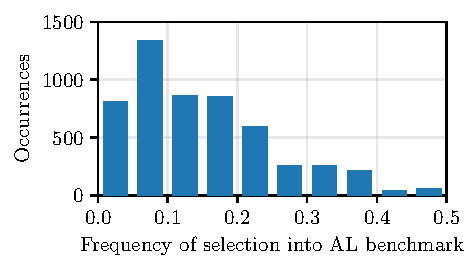
\includegraphics[width=0.6\textwidth]{plots/instoccs.pdf}
  \caption{Frequency with which individual problem instances are selected within all active-learning benchmarks. Instances that are chosen more frequently are intuitively more important for distinguishing solver runtimes. Results are on the full dataset with cross-validation over all solvers.}
  \label{fig:instoccs}
\end{figure}

\begin{figure}[tb]
  \centering
  \resizebox{0.85\textwidth}{!}{
    \graphicspath{{plots/}}
    %% Creator: Matplotlib, PGF backend
%%
%% To include the figure in your LaTeX document, write
%%   \input{<filename>.pgf}
%%
%% Make sure the required packages are loaded in your preamble
%%   \usepackage{pgf}
%%
%% Also ensure that all the required font packages are loaded; for instance,
%% the lmodern package is sometimes necessary when using math font.
%%   \usepackage{lmodern}
%%
%% Figures using additional raster images can only be included by \input if
%% they are in the same directory as the main LaTeX file. For loading figures
%% from other directories you can use the `import` package
%%   \usepackage{import}
%%
%% and then include the figures with
%%   \import{<path to file>}{<filename>.pgf}
%%
%% Matplotlib used the following preamble
%%
\begingroup%
\makeatletter%
\begin{pgfpicture}%
\pgfpathrectangle{\pgfpointorigin}{\pgfqpoint{6.617833in}{4.374364in}}%
\pgfusepath{use as bounding box, clip}%
\begin{pgfscope}%
\pgfsetbuttcap%
\pgfsetmiterjoin%
\pgfsetlinewidth{0.000000pt}%
\definecolor{currentstroke}{rgb}{1.000000,1.000000,1.000000}%
\pgfsetstrokecolor{currentstroke}%
\pgfsetstrokeopacity{0.000000}%
\pgfsetdash{}{0pt}%
\pgfpathmoveto{\pgfqpoint{0.000000in}{0.000000in}}%
\pgfpathlineto{\pgfqpoint{6.617833in}{0.000000in}}%
\pgfpathlineto{\pgfqpoint{6.617833in}{4.374364in}}%
\pgfpathlineto{\pgfqpoint{0.000000in}{4.374364in}}%
\pgfpathlineto{\pgfqpoint{0.000000in}{0.000000in}}%
\pgfpathclose%
\pgfusepath{}%
\end{pgfscope}%
\begin{pgfscope}%
\pgfsetbuttcap%
\pgfsetmiterjoin%
\definecolor{currentfill}{rgb}{1.000000,1.000000,1.000000}%
\pgfsetfillcolor{currentfill}%
\pgfsetlinewidth{0.000000pt}%
\definecolor{currentstroke}{rgb}{0.000000,0.000000,0.000000}%
\pgfsetstrokecolor{currentstroke}%
\pgfsetstrokeopacity{0.000000}%
\pgfsetdash{}{0pt}%
\pgfpathmoveto{\pgfqpoint{0.972719in}{0.707253in}}%
\pgfpathlineto{\pgfqpoint{6.320093in}{0.707253in}}%
\pgfpathlineto{\pgfqpoint{6.320093in}{4.191030in}}%
\pgfpathlineto{\pgfqpoint{0.972719in}{4.191030in}}%
\pgfpathlineto{\pgfqpoint{0.972719in}{0.707253in}}%
\pgfpathclose%
\pgfusepath{fill}%
\end{pgfscope}%
\begin{pgfscope}%
\pgfsetbuttcap%
\pgfsetroundjoin%
\definecolor{currentfill}{rgb}{0.000000,0.000000,0.000000}%
\pgfsetfillcolor{currentfill}%
\pgfsetlinewidth{0.803000pt}%
\definecolor{currentstroke}{rgb}{0.000000,0.000000,0.000000}%
\pgfsetstrokecolor{currentstroke}%
\pgfsetdash{}{0pt}%
\pgfsys@defobject{currentmarker}{\pgfqpoint{0.000000in}{-0.048611in}}{\pgfqpoint{0.000000in}{0.000000in}}{%
\pgfpathmoveto{\pgfqpoint{0.000000in}{0.000000in}}%
\pgfpathlineto{\pgfqpoint{0.000000in}{-0.048611in}}%
\pgfusepath{stroke,fill}%
}%
\begin{pgfscope}%
\pgfsys@transformshift{0.972719in}{0.707253in}%
\pgfsys@useobject{currentmarker}{}%
\end{pgfscope}%
\end{pgfscope}%
\begin{pgfscope}%
\definecolor{textcolor}{rgb}{0.000000,0.000000,0.000000}%
\pgfsetstrokecolor{textcolor}%
\pgfsetfillcolor{textcolor}%
\pgftext[x=0.972719in,y=0.610031in,,top]{\color{textcolor}\rmfamily\fontsize{18.000000}{21.600000}\selectfont \(\displaystyle {0.00}\)}%
\end{pgfscope}%
\begin{pgfscope}%
\pgfsetbuttcap%
\pgfsetroundjoin%
\definecolor{currentfill}{rgb}{0.000000,0.000000,0.000000}%
\pgfsetfillcolor{currentfill}%
\pgfsetlinewidth{0.803000pt}%
\definecolor{currentstroke}{rgb}{0.000000,0.000000,0.000000}%
\pgfsetstrokecolor{currentstroke}%
\pgfsetdash{}{0pt}%
\pgfsys@defobject{currentmarker}{\pgfqpoint{0.000000in}{-0.048611in}}{\pgfqpoint{0.000000in}{0.000000in}}{%
\pgfpathmoveto{\pgfqpoint{0.000000in}{0.000000in}}%
\pgfpathlineto{\pgfqpoint{0.000000in}{-0.048611in}}%
\pgfusepath{stroke,fill}%
}%
\begin{pgfscope}%
\pgfsys@transformshift{2.042194in}{0.707253in}%
\pgfsys@useobject{currentmarker}{}%
\end{pgfscope}%
\end{pgfscope}%
\begin{pgfscope}%
\definecolor{textcolor}{rgb}{0.000000,0.000000,0.000000}%
\pgfsetstrokecolor{textcolor}%
\pgfsetfillcolor{textcolor}%
\pgftext[x=2.042194in,y=0.610031in,,top]{\color{textcolor}\rmfamily\fontsize{18.000000}{21.600000}\selectfont \(\displaystyle {0.02}\)}%
\end{pgfscope}%
\begin{pgfscope}%
\pgfsetbuttcap%
\pgfsetroundjoin%
\definecolor{currentfill}{rgb}{0.000000,0.000000,0.000000}%
\pgfsetfillcolor{currentfill}%
\pgfsetlinewidth{0.803000pt}%
\definecolor{currentstroke}{rgb}{0.000000,0.000000,0.000000}%
\pgfsetstrokecolor{currentstroke}%
\pgfsetdash{}{0pt}%
\pgfsys@defobject{currentmarker}{\pgfqpoint{0.000000in}{-0.048611in}}{\pgfqpoint{0.000000in}{0.000000in}}{%
\pgfpathmoveto{\pgfqpoint{0.000000in}{0.000000in}}%
\pgfpathlineto{\pgfqpoint{0.000000in}{-0.048611in}}%
\pgfusepath{stroke,fill}%
}%
\begin{pgfscope}%
\pgfsys@transformshift{3.111668in}{0.707253in}%
\pgfsys@useobject{currentmarker}{}%
\end{pgfscope}%
\end{pgfscope}%
\begin{pgfscope}%
\definecolor{textcolor}{rgb}{0.000000,0.000000,0.000000}%
\pgfsetstrokecolor{textcolor}%
\pgfsetfillcolor{textcolor}%
\pgftext[x=3.111668in,y=0.610031in,,top]{\color{textcolor}\rmfamily\fontsize{18.000000}{21.600000}\selectfont \(\displaystyle {0.04}\)}%
\end{pgfscope}%
\begin{pgfscope}%
\pgfsetbuttcap%
\pgfsetroundjoin%
\definecolor{currentfill}{rgb}{0.000000,0.000000,0.000000}%
\pgfsetfillcolor{currentfill}%
\pgfsetlinewidth{0.803000pt}%
\definecolor{currentstroke}{rgb}{0.000000,0.000000,0.000000}%
\pgfsetstrokecolor{currentstroke}%
\pgfsetdash{}{0pt}%
\pgfsys@defobject{currentmarker}{\pgfqpoint{0.000000in}{-0.048611in}}{\pgfqpoint{0.000000in}{0.000000in}}{%
\pgfpathmoveto{\pgfqpoint{0.000000in}{0.000000in}}%
\pgfpathlineto{\pgfqpoint{0.000000in}{-0.048611in}}%
\pgfusepath{stroke,fill}%
}%
\begin{pgfscope}%
\pgfsys@transformshift{4.181143in}{0.707253in}%
\pgfsys@useobject{currentmarker}{}%
\end{pgfscope}%
\end{pgfscope}%
\begin{pgfscope}%
\definecolor{textcolor}{rgb}{0.000000,0.000000,0.000000}%
\pgfsetstrokecolor{textcolor}%
\pgfsetfillcolor{textcolor}%
\pgftext[x=4.181143in,y=0.610031in,,top]{\color{textcolor}\rmfamily\fontsize{18.000000}{21.600000}\selectfont \(\displaystyle {0.06}\)}%
\end{pgfscope}%
\begin{pgfscope}%
\pgfsetbuttcap%
\pgfsetroundjoin%
\definecolor{currentfill}{rgb}{0.000000,0.000000,0.000000}%
\pgfsetfillcolor{currentfill}%
\pgfsetlinewidth{0.803000pt}%
\definecolor{currentstroke}{rgb}{0.000000,0.000000,0.000000}%
\pgfsetstrokecolor{currentstroke}%
\pgfsetdash{}{0pt}%
\pgfsys@defobject{currentmarker}{\pgfqpoint{0.000000in}{-0.048611in}}{\pgfqpoint{0.000000in}{0.000000in}}{%
\pgfpathmoveto{\pgfqpoint{0.000000in}{0.000000in}}%
\pgfpathlineto{\pgfqpoint{0.000000in}{-0.048611in}}%
\pgfusepath{stroke,fill}%
}%
\begin{pgfscope}%
\pgfsys@transformshift{5.250618in}{0.707253in}%
\pgfsys@useobject{currentmarker}{}%
\end{pgfscope}%
\end{pgfscope}%
\begin{pgfscope}%
\definecolor{textcolor}{rgb}{0.000000,0.000000,0.000000}%
\pgfsetstrokecolor{textcolor}%
\pgfsetfillcolor{textcolor}%
\pgftext[x=5.250618in,y=0.610031in,,top]{\color{textcolor}\rmfamily\fontsize{18.000000}{21.600000}\selectfont \(\displaystyle {0.08}\)}%
\end{pgfscope}%
\begin{pgfscope}%
\pgfsetbuttcap%
\pgfsetroundjoin%
\definecolor{currentfill}{rgb}{0.000000,0.000000,0.000000}%
\pgfsetfillcolor{currentfill}%
\pgfsetlinewidth{0.803000pt}%
\definecolor{currentstroke}{rgb}{0.000000,0.000000,0.000000}%
\pgfsetstrokecolor{currentstroke}%
\pgfsetdash{}{0pt}%
\pgfsys@defobject{currentmarker}{\pgfqpoint{0.000000in}{-0.048611in}}{\pgfqpoint{0.000000in}{0.000000in}}{%
\pgfpathmoveto{\pgfqpoint{0.000000in}{0.000000in}}%
\pgfpathlineto{\pgfqpoint{0.000000in}{-0.048611in}}%
\pgfusepath{stroke,fill}%
}%
\begin{pgfscope}%
\pgfsys@transformshift{6.320093in}{0.707253in}%
\pgfsys@useobject{currentmarker}{}%
\end{pgfscope}%
\end{pgfscope}%
\begin{pgfscope}%
\definecolor{textcolor}{rgb}{0.000000,0.000000,0.000000}%
\pgfsetstrokecolor{textcolor}%
\pgfsetfillcolor{textcolor}%
\pgftext[x=6.320093in,y=0.610031in,,top]{\color{textcolor}\rmfamily\fontsize{18.000000}{21.600000}\selectfont \(\displaystyle {0.10}\)}%
\end{pgfscope}%
\begin{pgfscope}%
\definecolor{textcolor}{rgb}{0.000000,0.000000,0.000000}%
\pgfsetstrokecolor{textcolor}%
\pgfsetfillcolor{textcolor}%
\pgftext[x=3.646406in,y=0.313349in,,top]{\color{textcolor}\rmfamily\fontsize{18.000000}{21.600000}\selectfont Fraction in Dataset}%
\end{pgfscope}%
\begin{pgfscope}%
\pgfsetbuttcap%
\pgfsetroundjoin%
\definecolor{currentfill}{rgb}{0.000000,0.000000,0.000000}%
\pgfsetfillcolor{currentfill}%
\pgfsetlinewidth{0.803000pt}%
\definecolor{currentstroke}{rgb}{0.000000,0.000000,0.000000}%
\pgfsetstrokecolor{currentstroke}%
\pgfsetdash{}{0pt}%
\pgfsys@defobject{currentmarker}{\pgfqpoint{-0.048611in}{0.000000in}}{\pgfqpoint{-0.000000in}{0.000000in}}{%
\pgfpathmoveto{\pgfqpoint{-0.000000in}{0.000000in}}%
\pgfpathlineto{\pgfqpoint{-0.048611in}{0.000000in}}%
\pgfusepath{stroke,fill}%
}%
\begin{pgfscope}%
\pgfsys@transformshift{0.972719in}{0.707253in}%
\pgfsys@useobject{currentmarker}{}%
\end{pgfscope}%
\end{pgfscope}%
\begin{pgfscope}%
\definecolor{textcolor}{rgb}{0.000000,0.000000,0.000000}%
\pgfsetstrokecolor{textcolor}%
\pgfsetfillcolor{textcolor}%
\pgftext[x=0.480015in, y=0.623919in, left, base]{\color{textcolor}\rmfamily\fontsize{18.000000}{21.600000}\selectfont \(\displaystyle {0.00}\)}%
\end{pgfscope}%
\begin{pgfscope}%
\pgfsetbuttcap%
\pgfsetroundjoin%
\definecolor{currentfill}{rgb}{0.000000,0.000000,0.000000}%
\pgfsetfillcolor{currentfill}%
\pgfsetlinewidth{0.803000pt}%
\definecolor{currentstroke}{rgb}{0.000000,0.000000,0.000000}%
\pgfsetstrokecolor{currentstroke}%
\pgfsetdash{}{0pt}%
\pgfsys@defobject{currentmarker}{\pgfqpoint{-0.048611in}{0.000000in}}{\pgfqpoint{-0.000000in}{0.000000in}}{%
\pgfpathmoveto{\pgfqpoint{-0.000000in}{0.000000in}}%
\pgfpathlineto{\pgfqpoint{-0.048611in}{0.000000in}}%
\pgfusepath{stroke,fill}%
}%
\begin{pgfscope}%
\pgfsys@transformshift{0.972719in}{1.404008in}%
\pgfsys@useobject{currentmarker}{}%
\end{pgfscope}%
\end{pgfscope}%
\begin{pgfscope}%
\definecolor{textcolor}{rgb}{0.000000,0.000000,0.000000}%
\pgfsetstrokecolor{textcolor}%
\pgfsetfillcolor{textcolor}%
\pgftext[x=0.480015in, y=1.320675in, left, base]{\color{textcolor}\rmfamily\fontsize{18.000000}{21.600000}\selectfont \(\displaystyle {0.02}\)}%
\end{pgfscope}%
\begin{pgfscope}%
\pgfsetbuttcap%
\pgfsetroundjoin%
\definecolor{currentfill}{rgb}{0.000000,0.000000,0.000000}%
\pgfsetfillcolor{currentfill}%
\pgfsetlinewidth{0.803000pt}%
\definecolor{currentstroke}{rgb}{0.000000,0.000000,0.000000}%
\pgfsetstrokecolor{currentstroke}%
\pgfsetdash{}{0pt}%
\pgfsys@defobject{currentmarker}{\pgfqpoint{-0.048611in}{0.000000in}}{\pgfqpoint{-0.000000in}{0.000000in}}{%
\pgfpathmoveto{\pgfqpoint{-0.000000in}{0.000000in}}%
\pgfpathlineto{\pgfqpoint{-0.048611in}{0.000000in}}%
\pgfusepath{stroke,fill}%
}%
\begin{pgfscope}%
\pgfsys@transformshift{0.972719in}{2.100764in}%
\pgfsys@useobject{currentmarker}{}%
\end{pgfscope}%
\end{pgfscope}%
\begin{pgfscope}%
\definecolor{textcolor}{rgb}{0.000000,0.000000,0.000000}%
\pgfsetstrokecolor{textcolor}%
\pgfsetfillcolor{textcolor}%
\pgftext[x=0.480015in, y=2.017430in, left, base]{\color{textcolor}\rmfamily\fontsize{18.000000}{21.600000}\selectfont \(\displaystyle {0.04}\)}%
\end{pgfscope}%
\begin{pgfscope}%
\pgfsetbuttcap%
\pgfsetroundjoin%
\definecolor{currentfill}{rgb}{0.000000,0.000000,0.000000}%
\pgfsetfillcolor{currentfill}%
\pgfsetlinewidth{0.803000pt}%
\definecolor{currentstroke}{rgb}{0.000000,0.000000,0.000000}%
\pgfsetstrokecolor{currentstroke}%
\pgfsetdash{}{0pt}%
\pgfsys@defobject{currentmarker}{\pgfqpoint{-0.048611in}{0.000000in}}{\pgfqpoint{-0.000000in}{0.000000in}}{%
\pgfpathmoveto{\pgfqpoint{-0.000000in}{0.000000in}}%
\pgfpathlineto{\pgfqpoint{-0.048611in}{0.000000in}}%
\pgfusepath{stroke,fill}%
}%
\begin{pgfscope}%
\pgfsys@transformshift{0.972719in}{2.797519in}%
\pgfsys@useobject{currentmarker}{}%
\end{pgfscope}%
\end{pgfscope}%
\begin{pgfscope}%
\definecolor{textcolor}{rgb}{0.000000,0.000000,0.000000}%
\pgfsetstrokecolor{textcolor}%
\pgfsetfillcolor{textcolor}%
\pgftext[x=0.480015in, y=2.714186in, left, base]{\color{textcolor}\rmfamily\fontsize{18.000000}{21.600000}\selectfont \(\displaystyle {0.06}\)}%
\end{pgfscope}%
\begin{pgfscope}%
\pgfsetbuttcap%
\pgfsetroundjoin%
\definecolor{currentfill}{rgb}{0.000000,0.000000,0.000000}%
\pgfsetfillcolor{currentfill}%
\pgfsetlinewidth{0.803000pt}%
\definecolor{currentstroke}{rgb}{0.000000,0.000000,0.000000}%
\pgfsetstrokecolor{currentstroke}%
\pgfsetdash{}{0pt}%
\pgfsys@defobject{currentmarker}{\pgfqpoint{-0.048611in}{0.000000in}}{\pgfqpoint{-0.000000in}{0.000000in}}{%
\pgfpathmoveto{\pgfqpoint{-0.000000in}{0.000000in}}%
\pgfpathlineto{\pgfqpoint{-0.048611in}{0.000000in}}%
\pgfusepath{stroke,fill}%
}%
\begin{pgfscope}%
\pgfsys@transformshift{0.972719in}{3.494275in}%
\pgfsys@useobject{currentmarker}{}%
\end{pgfscope}%
\end{pgfscope}%
\begin{pgfscope}%
\definecolor{textcolor}{rgb}{0.000000,0.000000,0.000000}%
\pgfsetstrokecolor{textcolor}%
\pgfsetfillcolor{textcolor}%
\pgftext[x=0.480015in, y=3.410942in, left, base]{\color{textcolor}\rmfamily\fontsize{18.000000}{21.600000}\selectfont \(\displaystyle {0.08}\)}%
\end{pgfscope}%
\begin{pgfscope}%
\pgfsetbuttcap%
\pgfsetroundjoin%
\definecolor{currentfill}{rgb}{0.000000,0.000000,0.000000}%
\pgfsetfillcolor{currentfill}%
\pgfsetlinewidth{0.803000pt}%
\definecolor{currentstroke}{rgb}{0.000000,0.000000,0.000000}%
\pgfsetstrokecolor{currentstroke}%
\pgfsetdash{}{0pt}%
\pgfsys@defobject{currentmarker}{\pgfqpoint{-0.048611in}{0.000000in}}{\pgfqpoint{-0.000000in}{0.000000in}}{%
\pgfpathmoveto{\pgfqpoint{-0.000000in}{0.000000in}}%
\pgfpathlineto{\pgfqpoint{-0.048611in}{0.000000in}}%
\pgfusepath{stroke,fill}%
}%
\begin{pgfscope}%
\pgfsys@transformshift{0.972719in}{4.191030in}%
\pgfsys@useobject{currentmarker}{}%
\end{pgfscope}%
\end{pgfscope}%
\begin{pgfscope}%
\definecolor{textcolor}{rgb}{0.000000,0.000000,0.000000}%
\pgfsetstrokecolor{textcolor}%
\pgfsetfillcolor{textcolor}%
\pgftext[x=0.480015in, y=4.107697in, left, base]{\color{textcolor}\rmfamily\fontsize{18.000000}{21.600000}\selectfont \(\displaystyle {0.10}\)}%
\end{pgfscope}%
\begin{pgfscope}%
\definecolor{textcolor}{rgb}{0.000000,0.000000,0.000000}%
\pgfsetstrokecolor{textcolor}%
\pgfsetfillcolor{textcolor}%
\pgftext[x=0.313349in,y=2.449142in,,bottom,rotate=90.000000]{\color{textcolor}\rmfamily\fontsize{18.000000}{21.600000}\selectfont Fraction in Selected Benchmark}%
\end{pgfscope}%
\begin{pgfscope}%
\pgfsetrectcap%
\pgfsetmiterjoin%
\pgfsetlinewidth{0.803000pt}%
\definecolor{currentstroke}{rgb}{0.000000,0.000000,0.000000}%
\pgfsetstrokecolor{currentstroke}%
\pgfsetdash{}{0pt}%
\pgfpathmoveto{\pgfqpoint{0.972719in}{0.707253in}}%
\pgfpathlineto{\pgfqpoint{0.972719in}{4.191030in}}%
\pgfusepath{stroke}%
\end{pgfscope}%
\begin{pgfscope}%
\pgfsetrectcap%
\pgfsetmiterjoin%
\pgfsetlinewidth{0.803000pt}%
\definecolor{currentstroke}{rgb}{0.000000,0.000000,0.000000}%
\pgfsetstrokecolor{currentstroke}%
\pgfsetdash{}{0pt}%
\pgfpathmoveto{\pgfqpoint{6.320093in}{0.707253in}}%
\pgfpathlineto{\pgfqpoint{6.320093in}{4.191030in}}%
\pgfusepath{stroke}%
\end{pgfscope}%
\begin{pgfscope}%
\pgfsetrectcap%
\pgfsetmiterjoin%
\pgfsetlinewidth{0.803000pt}%
\definecolor{currentstroke}{rgb}{0.000000,0.000000,0.000000}%
\pgfsetstrokecolor{currentstroke}%
\pgfsetdash{}{0pt}%
\pgfpathmoveto{\pgfqpoint{0.972719in}{0.707253in}}%
\pgfpathlineto{\pgfqpoint{6.320093in}{0.707253in}}%
\pgfusepath{stroke}%
\end{pgfscope}%
\begin{pgfscope}%
\pgfsetrectcap%
\pgfsetmiterjoin%
\pgfsetlinewidth{0.803000pt}%
\definecolor{currentstroke}{rgb}{0.000000,0.000000,0.000000}%
\pgfsetstrokecolor{currentstroke}%
\pgfsetdash{}{0pt}%
\pgfpathmoveto{\pgfqpoint{0.972719in}{4.191030in}}%
\pgfpathlineto{\pgfqpoint{6.320093in}{4.191030in}}%
\pgfusepath{stroke}%
\end{pgfscope}%
\begin{pgfscope}%
\definecolor{textcolor}{rgb}{0.000000,0.000000,0.000000}%
\pgfsetstrokecolor{textcolor}%
\pgfsetfillcolor{textcolor}%
\pgftext[x=3.325563in,y=3.556983in,left,base]{\color{textcolor}\rmfamily\fontsize{16.000000}{19.200000}\selectfont planning}%
\end{pgfscope}%
\begin{pgfscope}%
\definecolor{textcolor}{rgb}{0.000000,0.000000,0.000000}%
\pgfsetstrokecolor{textcolor}%
\pgfsetfillcolor{textcolor}%
\pgftext[x=4.608933in,y=2.884614in,left,base]{\color{textcolor}\rmfamily\fontsize{16.000000}{19.200000}\selectfont hardware-verific.}%
\end{pgfscope}%
\begin{pgfscope}%
\definecolor{textcolor}{rgb}{0.000000,0.000000,0.000000}%
\pgfsetstrokecolor{textcolor}%
\pgfsetfillcolor{textcolor}%
\pgftext[x=1.186614in,y=2.666878in,left,base]{\color{textcolor}\rmfamily\fontsize{16.000000}{19.200000}\selectfont quasigroup-compl.}%
\end{pgfscope}%
\begin{pgfscope}%
\definecolor{textcolor}{rgb}{0.000000,0.000000,0.000000}%
\pgfsetstrokecolor{textcolor}%
\pgfsetfillcolor{textcolor}%
\pgftext[x=4.256006in,y=2.335919in,left,base]{\color{textcolor}\rmfamily\fontsize{16.000000}{19.200000}\selectfont cryptography}%
\end{pgfscope}%
\begin{pgfscope}%
\definecolor{textcolor}{rgb}{0.000000,0.000000,0.000000}%
\pgfsetstrokecolor{textcolor}%
\pgfsetfillcolor{textcolor}%
\pgftext[x=1.133140in,y=1.539876in,left,base]{\color{textcolor}\rmfamily\fontsize{16.000000}{19.200000}\selectfont fpga}%
\end{pgfscope}%
\begin{pgfscope}%
\pgfpathrectangle{\pgfqpoint{0.972719in}{0.707253in}}{\pgfqpoint{5.347374in}{3.483778in}}%
\pgfusepath{clip}%
\pgfsetbuttcap%
\pgfsetroundjoin%
\pgfsetlinewidth{1.505625pt}%
\definecolor{currentstroke}{rgb}{0.501961,0.501961,0.501961}%
\pgfsetstrokecolor{currentstroke}%
\pgfsetstrokeopacity{0.400000}%
\pgfsetdash{{5.550000pt}{2.400000pt}}{0.000000pt}%
\pgfpathmoveto{\pgfqpoint{0.972719in}{0.707253in}}%
\pgfpathlineto{\pgfqpoint{6.328426in}{4.196459in}}%
\pgfusepath{stroke}%
\end{pgfscope}%
\begin{pgfscope}%
\pgfpathrectangle{\pgfqpoint{0.972719in}{0.707253in}}{\pgfqpoint{5.347374in}{3.483778in}}%
\pgfusepath{clip}%
\pgfsetbuttcap%
\pgfsetroundjoin%
\definecolor{currentfill}{rgb}{0.121569,0.466667,0.705882}%
\pgfsetfillcolor{currentfill}%
\pgfsetfillopacity{0.800000}%
\pgfsetlinewidth{1.003750pt}%
\definecolor{currentstroke}{rgb}{0.121569,0.466667,0.705882}%
\pgfsetstrokecolor{currentstroke}%
\pgfsetstrokeopacity{0.800000}%
\pgfsetdash{}{0pt}%
\pgfsys@defobject{currentmarker}{\pgfqpoint{-0.049105in}{-0.049105in}}{\pgfqpoint{0.049105in}{0.049105in}}{%
\pgfpathmoveto{\pgfqpoint{0.000000in}{-0.049105in}}%
\pgfpathcurveto{\pgfqpoint{0.013023in}{-0.049105in}}{\pgfqpoint{0.025514in}{-0.043931in}}{\pgfqpoint{0.034722in}{-0.034722in}}%
\pgfpathcurveto{\pgfqpoint{0.043931in}{-0.025514in}}{\pgfqpoint{0.049105in}{-0.013023in}}{\pgfqpoint{0.049105in}{0.000000in}}%
\pgfpathcurveto{\pgfqpoint{0.049105in}{0.013023in}}{\pgfqpoint{0.043931in}{0.025514in}}{\pgfqpoint{0.034722in}{0.034722in}}%
\pgfpathcurveto{\pgfqpoint{0.025514in}{0.043931in}}{\pgfqpoint{0.013023in}{0.049105in}}{\pgfqpoint{0.000000in}{0.049105in}}%
\pgfpathcurveto{\pgfqpoint{-0.013023in}{0.049105in}}{\pgfqpoint{-0.025514in}{0.043931in}}{\pgfqpoint{-0.034722in}{0.034722in}}%
\pgfpathcurveto{\pgfqpoint{-0.043931in}{0.025514in}}{\pgfqpoint{-0.049105in}{0.013023in}}{\pgfqpoint{-0.049105in}{0.000000in}}%
\pgfpathcurveto{\pgfqpoint{-0.049105in}{-0.013023in}}{\pgfqpoint{-0.043931in}{-0.025514in}}{\pgfqpoint{-0.034722in}{-0.034722in}}%
\pgfpathcurveto{\pgfqpoint{-0.025514in}{-0.043931in}}{\pgfqpoint{-0.013023in}{-0.049105in}}{\pgfqpoint{0.000000in}{-0.049105in}}%
\pgfpathlineto{\pgfqpoint{0.000000in}{-0.049105in}}%
\pgfpathclose%
\pgfusepath{stroke,fill}%
}%
\begin{pgfscope}%
\pgfsys@transformshift{0.992894in}{0.718685in}%
\pgfsys@useobject{currentmarker}{}%
\end{pgfscope}%
\begin{pgfscope}%
\pgfsys@transformshift{1.234994in}{0.947865in}%
\pgfsys@useobject{currentmarker}{}%
\end{pgfscope}%
\begin{pgfscope}%
\pgfsys@transformshift{1.033244in}{0.741336in}%
\pgfsys@useobject{currentmarker}{}%
\end{pgfscope}%
\begin{pgfscope}%
\pgfsys@transformshift{1.103856in}{0.800848in}%
\pgfsys@useobject{currentmarker}{}%
\end{pgfscope}%
\begin{pgfscope}%
\pgfsys@transformshift{1.255168in}{0.908012in}%
\pgfsys@useobject{currentmarker}{}%
\end{pgfscope}%
\begin{pgfscope}%
\pgfsys@transformshift{1.103856in}{0.773389in}%
\pgfsys@useobject{currentmarker}{}%
\end{pgfscope}%
\begin{pgfscope}%
\pgfsys@transformshift{1.436743in}{0.924573in}%
\pgfsys@useobject{currentmarker}{}%
\end{pgfscope}%
\begin{pgfscope}%
\pgfsys@transformshift{1.083681in}{0.774778in}%
\pgfsys@useobject{currentmarker}{}%
\end{pgfscope}%
\begin{pgfscope}%
\pgfsys@transformshift{1.103856in}{0.777449in}%
\pgfsys@useobject{currentmarker}{}%
\end{pgfscope}%
\begin{pgfscope}%
\pgfsys@transformshift{1.295518in}{1.017634in}%
\pgfsys@useobject{currentmarker}{}%
\end{pgfscope}%
\begin{pgfscope}%
\pgfsys@transformshift{1.446831in}{0.985794in}%
\pgfsys@useobject{currentmarker}{}%
\end{pgfscope}%
\begin{pgfscope}%
\pgfsys@transformshift{3.131440in}{2.013096in}%
\pgfsys@useobject{currentmarker}{}%
\end{pgfscope}%
\begin{pgfscope}%
\pgfsys@transformshift{1.113944in}{0.849462in}%
\pgfsys@useobject{currentmarker}{}%
\end{pgfscope}%
\begin{pgfscope}%
\pgfsys@transformshift{1.124031in}{0.785676in}%
\pgfsys@useobject{currentmarker}{}%
\end{pgfscope}%
\begin{pgfscope}%
\pgfsys@transformshift{1.325781in}{0.883865in}%
\pgfsys@useobject{currentmarker}{}%
\end{pgfscope}%
\begin{pgfscope}%
\pgfsys@transformshift{1.023156in}{0.737169in}%
\pgfsys@useobject{currentmarker}{}%
\end{pgfscope}%
\begin{pgfscope}%
\pgfsys@transformshift{0.992894in}{0.717830in}%
\pgfsys@useobject{currentmarker}{}%
\end{pgfscope}%
\begin{pgfscope}%
\pgfsys@transformshift{1.063506in}{0.789416in}%
\pgfsys@useobject{currentmarker}{}%
\end{pgfscope}%
\begin{pgfscope}%
\pgfsys@transformshift{1.618318in}{1.135589in}%
\pgfsys@useobject{currentmarker}{}%
\end{pgfscope}%
\begin{pgfscope}%
\pgfsys@transformshift{1.224906in}{0.848928in}%
\pgfsys@useobject{currentmarker}{}%
\end{pgfscope}%
\begin{pgfscope}%
\pgfsys@transformshift{1.043331in}{0.747853in}%
\pgfsys@useobject{currentmarker}{}%
\end{pgfscope}%
\begin{pgfscope}%
\pgfsys@transformshift{1.386306in}{0.994876in}%
\pgfsys@useobject{currentmarker}{}%
\end{pgfscope}%
\begin{pgfscope}%
\pgfsys@transformshift{1.103856in}{0.782791in}%
\pgfsys@useobject{currentmarker}{}%
\end{pgfscope}%
\begin{pgfscope}%
\pgfsys@transformshift{1.103856in}{0.796360in}%
\pgfsys@useobject{currentmarker}{}%
\end{pgfscope}%
\begin{pgfscope}%
\pgfsys@transformshift{1.164381in}{0.786317in}%
\pgfsys@useobject{currentmarker}{}%
\end{pgfscope}%
\begin{pgfscope}%
\pgfsys@transformshift{4.109926in}{2.385126in}%
\pgfsys@useobject{currentmarker}{}%
\end{pgfscope}%
\begin{pgfscope}%
\pgfsys@transformshift{0.992894in}{0.724134in}%
\pgfsys@useobject{currentmarker}{}%
\end{pgfscope}%
\begin{pgfscope}%
\pgfsys@transformshift{2.122692in}{1.377270in}%
\pgfsys@useobject{currentmarker}{}%
\end{pgfscope}%
\begin{pgfscope}%
\pgfsys@transformshift{1.245081in}{1.005774in}%
\pgfsys@useobject{currentmarker}{}%
\end{pgfscope}%
\begin{pgfscope}%
\pgfsys@transformshift{1.043331in}{0.740374in}%
\pgfsys@useobject{currentmarker}{}%
\end{pgfscope}%
\begin{pgfscope}%
\pgfsys@transformshift{1.416568in}{0.978315in}%
\pgfsys@useobject{currentmarker}{}%
\end{pgfscope}%
\begin{pgfscope}%
\pgfsys@transformshift{1.103856in}{0.772107in}%
\pgfsys@useobject{currentmarker}{}%
\end{pgfscope}%
\begin{pgfscope}%
\pgfsys@transformshift{1.103856in}{0.771038in}%
\pgfsys@useobject{currentmarker}{}%
\end{pgfscope}%
\begin{pgfscope}%
\pgfsys@transformshift{1.073594in}{0.739947in}%
\pgfsys@useobject{currentmarker}{}%
\end{pgfscope}%
\begin{pgfscope}%
\pgfsys@transformshift{1.174469in}{0.810143in}%
\pgfsys@useobject{currentmarker}{}%
\end{pgfscope}%
\begin{pgfscope}%
\pgfsys@transformshift{1.113944in}{0.784821in}%
\pgfsys@useobject{currentmarker}{}%
\end{pgfscope}%
\begin{pgfscope}%
\pgfsys@transformshift{1.477093in}{1.217325in}%
\pgfsys@useobject{currentmarker}{}%
\end{pgfscope}%
\begin{pgfscope}%
\pgfsys@transformshift{1.023156in}{0.730224in}%
\pgfsys@useobject{currentmarker}{}%
\end{pgfscope}%
\begin{pgfscope}%
\pgfsys@transformshift{1.063506in}{0.793903in}%
\pgfsys@useobject{currentmarker}{}%
\end{pgfscope}%
\begin{pgfscope}%
\pgfsys@transformshift{1.234994in}{0.848928in}%
\pgfsys@useobject{currentmarker}{}%
\end{pgfscope}%
\begin{pgfscope}%
\pgfsys@transformshift{1.709105in}{1.574824in}%
\pgfsys@useobject{currentmarker}{}%
\end{pgfscope}%
\begin{pgfscope}%
\pgfsys@transformshift{1.426656in}{0.998829in}%
\pgfsys@useobject{currentmarker}{}%
\end{pgfscope}%
\begin{pgfscope}%
\pgfsys@transformshift{1.093769in}{0.859291in}%
\pgfsys@useobject{currentmarker}{}%
\end{pgfscope}%
\begin{pgfscope}%
\pgfsys@transformshift{0.982807in}{0.716441in}%
\pgfsys@useobject{currentmarker}{}%
\end{pgfscope}%
\begin{pgfscope}%
\pgfsys@transformshift{1.164381in}{0.782043in}%
\pgfsys@useobject{currentmarker}{}%
\end{pgfscope}%
\begin{pgfscope}%
\pgfsys@transformshift{2.324441in}{1.717780in}%
\pgfsys@useobject{currentmarker}{}%
\end{pgfscope}%
\begin{pgfscope}%
\pgfsys@transformshift{1.850330in}{1.424388in}%
\pgfsys@useobject{currentmarker}{}%
\end{pgfscope}%
\begin{pgfscope}%
\pgfsys@transformshift{1.588055in}{0.945514in}%
\pgfsys@useobject{currentmarker}{}%
\end{pgfscope}%
\begin{pgfscope}%
\pgfsys@transformshift{1.315693in}{0.944232in}%
\pgfsys@useobject{currentmarker}{}%
\end{pgfscope}%
\begin{pgfscope}%
\pgfsys@transformshift{1.073594in}{0.758751in}%
\pgfsys@useobject{currentmarker}{}%
\end{pgfscope}%
\begin{pgfscope}%
\pgfsys@transformshift{1.103856in}{0.773068in}%
\pgfsys@useobject{currentmarker}{}%
\end{pgfscope}%
\begin{pgfscope}%
\pgfsys@transformshift{1.023156in}{0.752875in}%
\pgfsys@useobject{currentmarker}{}%
\end{pgfscope}%
\begin{pgfscope}%
\pgfsys@transformshift{1.759543in}{1.160484in}%
\pgfsys@useobject{currentmarker}{}%
\end{pgfscope}%
\begin{pgfscope}%
\pgfsys@transformshift{4.442812in}{2.938149in}%
\pgfsys@useobject{currentmarker}{}%
\end{pgfscope}%
\begin{pgfscope}%
\pgfsys@transformshift{1.426656in}{0.939104in}%
\pgfsys@useobject{currentmarker}{}%
\end{pgfscope}%
\begin{pgfscope}%
\pgfsys@transformshift{1.124031in}{0.775419in}%
\pgfsys@useobject{currentmarker}{}%
\end{pgfscope}%
\begin{pgfscope}%
\pgfsys@transformshift{1.245081in}{0.847432in}%
\pgfsys@useobject{currentmarker}{}%
\end{pgfscope}%
\begin{pgfscope}%
\pgfsys@transformshift{1.113944in}{0.770932in}%
\pgfsys@useobject{currentmarker}{}%
\end{pgfscope}%
\begin{pgfscope}%
\pgfsys@transformshift{0.992894in}{0.716334in}%
\pgfsys@useobject{currentmarker}{}%
\end{pgfscope}%
\begin{pgfscope}%
\pgfsys@transformshift{1.144206in}{0.838564in}%
\pgfsys@useobject{currentmarker}{}%
\end{pgfscope}%
\begin{pgfscope}%
\pgfsys@transformshift{1.093769in}{0.764628in}%
\pgfsys@useobject{currentmarker}{}%
\end{pgfscope}%
\begin{pgfscope}%
\pgfsys@transformshift{1.033244in}{0.728728in}%
\pgfsys@useobject{currentmarker}{}%
\end{pgfscope}%
\begin{pgfscope}%
\pgfsys@transformshift{1.053419in}{0.764200in}%
\pgfsys@useobject{currentmarker}{}%
\end{pgfscope}%
\begin{pgfscope}%
\pgfsys@transformshift{1.033244in}{0.727446in}%
\pgfsys@useobject{currentmarker}{}%
\end{pgfscope}%
\begin{pgfscope}%
\pgfsys@transformshift{1.265256in}{0.899571in}%
\pgfsys@useobject{currentmarker}{}%
\end{pgfscope}%
\begin{pgfscope}%
\pgfsys@transformshift{0.992894in}{0.721142in}%
\pgfsys@useobject{currentmarker}{}%
\end{pgfscope}%
\begin{pgfscope}%
\pgfsys@transformshift{1.103856in}{0.771786in}%
\pgfsys@useobject{currentmarker}{}%
\end{pgfscope}%
\begin{pgfscope}%
\pgfsys@transformshift{1.134119in}{0.853842in}%
\pgfsys@useobject{currentmarker}{}%
\end{pgfscope}%
\begin{pgfscope}%
\pgfsys@transformshift{1.103856in}{0.786744in}%
\pgfsys@useobject{currentmarker}{}%
\end{pgfscope}%
\begin{pgfscope}%
\pgfsys@transformshift{1.033244in}{0.744969in}%
\pgfsys@useobject{currentmarker}{}%
\end{pgfscope}%
\begin{pgfscope}%
\pgfsys@transformshift{2.980128in}{1.985424in}%
\pgfsys@useobject{currentmarker}{}%
\end{pgfscope}%
\begin{pgfscope}%
\pgfsys@transformshift{1.144206in}{0.819118in}%
\pgfsys@useobject{currentmarker}{}%
\end{pgfscope}%
\begin{pgfscope}%
\pgfsys@transformshift{1.093769in}{0.783219in}%
\pgfsys@useobject{currentmarker}{}%
\end{pgfscope}%
\begin{pgfscope}%
\pgfsys@transformshift{1.285431in}{0.965173in}%
\pgfsys@useobject{currentmarker}{}%
\end{pgfscope}%
\begin{pgfscope}%
\pgfsys@transformshift{1.073594in}{0.782791in}%
\pgfsys@useobject{currentmarker}{}%
\end{pgfscope}%
\begin{pgfscope}%
\pgfsys@transformshift{1.063506in}{0.746678in}%
\pgfsys@useobject{currentmarker}{}%
\end{pgfscope}%
\begin{pgfscope}%
\pgfsys@transformshift{1.265256in}{0.981414in}%
\pgfsys@useobject{currentmarker}{}%
\end{pgfscope}%
\begin{pgfscope}%
\pgfsys@transformshift{1.255168in}{0.961007in}%
\pgfsys@useobject{currentmarker}{}%
\end{pgfscope}%
\begin{pgfscope}%
\pgfsys@transformshift{1.396393in}{1.033233in}%
\pgfsys@useobject{currentmarker}{}%
\end{pgfscope}%
\begin{pgfscope}%
\pgfsys@transformshift{1.063506in}{0.742618in}%
\pgfsys@useobject{currentmarker}{}%
\end{pgfscope}%
\begin{pgfscope}%
\pgfsys@transformshift{1.224906in}{0.880233in}%
\pgfsys@useobject{currentmarker}{}%
\end{pgfscope}%
\begin{pgfscope}%
\pgfsys@transformshift{1.144206in}{0.780761in}%
\pgfsys@useobject{currentmarker}{}%
\end{pgfscope}%
\begin{pgfscope}%
\pgfsys@transformshift{2.495929in}{1.615852in}%
\pgfsys@useobject{currentmarker}{}%
\end{pgfscope}%
\begin{pgfscope}%
\pgfsys@transformshift{4.331850in}{3.604320in}%
\pgfsys@useobject{currentmarker}{}%
\end{pgfscope}%
\begin{pgfscope}%
\pgfsys@transformshift{1.436743in}{0.982375in}%
\pgfsys@useobject{currentmarker}{}%
\end{pgfscope}%
\begin{pgfscope}%
\pgfsys@transformshift{1.376218in}{0.835893in}%
\pgfsys@useobject{currentmarker}{}%
\end{pgfscope}%
\begin{pgfscope}%
\pgfsys@transformshift{1.456918in}{0.989106in}%
\pgfsys@useobject{currentmarker}{}%
\end{pgfscope}%
\begin{pgfscope}%
\pgfsys@transformshift{1.487181in}{1.064431in}%
\pgfsys@useobject{currentmarker}{}%
\end{pgfscope}%
\begin{pgfscope}%
\pgfsys@transformshift{1.023156in}{0.761743in}%
\pgfsys@useobject{currentmarker}{}%
\end{pgfscope}%
\begin{pgfscope}%
\pgfsys@transformshift{1.124031in}{0.802878in}%
\pgfsys@useobject{currentmarker}{}%
\end{pgfscope}%
\begin{pgfscope}%
\pgfsys@transformshift{1.174469in}{0.806297in}%
\pgfsys@useobject{currentmarker}{}%
\end{pgfscope}%
\begin{pgfscope}%
\pgfsys@transformshift{1.184556in}{0.844226in}%
\pgfsys@useobject{currentmarker}{}%
\end{pgfscope}%
\begin{pgfscope}%
\pgfsys@transformshift{3.091090in}{2.709183in}%
\pgfsys@useobject{currentmarker}{}%
\end{pgfscope}%
\begin{pgfscope}%
\pgfsys@transformshift{0.982807in}{0.712061in}%
\pgfsys@useobject{currentmarker}{}%
\end{pgfscope}%
\begin{pgfscope}%
\pgfsys@transformshift{1.043331in}{0.771573in}%
\pgfsys@useobject{currentmarker}{}%
\end{pgfscope}%
\begin{pgfscope}%
\pgfsys@transformshift{1.053419in}{0.783860in}%
\pgfsys@useobject{currentmarker}{}%
\end{pgfscope}%
\begin{pgfscope}%
\pgfsys@transformshift{1.154294in}{0.843585in}%
\pgfsys@useobject{currentmarker}{}%
\end{pgfscope}%
\begin{pgfscope}%
\pgfsys@transformshift{1.204731in}{0.856407in}%
\pgfsys@useobject{currentmarker}{}%
\end{pgfscope}%
\begin{pgfscope}%
\pgfsys@transformshift{1.002981in}{0.716762in}%
\pgfsys@useobject{currentmarker}{}%
\end{pgfscope}%
\begin{pgfscope}%
\pgfsys@transformshift{1.547705in}{1.110481in}%
\pgfsys@useobject{currentmarker}{}%
\end{pgfscope}%
\begin{pgfscope}%
\pgfsys@transformshift{1.053419in}{0.742191in}%
\pgfsys@useobject{currentmarker}{}%
\end{pgfscope}%
\begin{pgfscope}%
\pgfsys@transformshift{2.112604in}{1.328228in}%
\pgfsys@useobject{currentmarker}{}%
\end{pgfscope}%
\begin{pgfscope}%
\pgfsys@transformshift{1.063506in}{0.769756in}%
\pgfsys@useobject{currentmarker}{}%
\end{pgfscope}%
\begin{pgfscope}%
\pgfsys@transformshift{1.245081in}{0.843051in}%
\pgfsys@useobject{currentmarker}{}%
\end{pgfscope}%
\begin{pgfscope}%
\pgfsys@transformshift{1.063506in}{0.741870in}%
\pgfsys@useobject{currentmarker}{}%
\end{pgfscope}%
\begin{pgfscope}%
\pgfsys@transformshift{2.052079in}{1.206213in}%
\pgfsys@useobject{currentmarker}{}%
\end{pgfscope}%
\begin{pgfscope}%
\pgfsys@transformshift{1.467006in}{0.941775in}%
\pgfsys@useobject{currentmarker}{}%
\end{pgfscope}%
\begin{pgfscope}%
\pgfsys@transformshift{1.598143in}{1.026929in}%
\pgfsys@useobject{currentmarker}{}%
\end{pgfscope}%
\begin{pgfscope}%
\pgfsys@transformshift{1.002981in}{0.727446in}%
\pgfsys@useobject{currentmarker}{}%
\end{pgfscope}%
\begin{pgfscope}%
\pgfsys@transformshift{1.083681in}{0.788561in}%
\pgfsys@useobject{currentmarker}{}%
\end{pgfscope}%
\begin{pgfscope}%
\pgfsys@transformshift{1.063506in}{0.766230in}%
\pgfsys@useobject{currentmarker}{}%
\end{pgfscope}%
\begin{pgfscope}%
\pgfsys@transformshift{1.073594in}{0.787706in}%
\pgfsys@useobject{currentmarker}{}%
\end{pgfscope}%
\begin{pgfscope}%
\pgfsys@transformshift{2.304267in}{1.495118in}%
\pgfsys@useobject{currentmarker}{}%
\end{pgfscope}%
\begin{pgfscope}%
\pgfsys@transformshift{1.174469in}{0.830230in}%
\pgfsys@useobject{currentmarker}{}%
\end{pgfscope}%
\begin{pgfscope}%
\pgfsys@transformshift{1.093769in}{0.789843in}%
\pgfsys@useobject{currentmarker}{}%
\end{pgfscope}%
\begin{pgfscope}%
\pgfsys@transformshift{0.992894in}{0.726378in}%
\pgfsys@useobject{currentmarker}{}%
\end{pgfscope}%
\begin{pgfscope}%
\pgfsys@transformshift{1.376218in}{0.908012in}%
\pgfsys@useobject{currentmarker}{}%
\end{pgfscope}%
\begin{pgfscope}%
\pgfsys@transformshift{1.083681in}{0.781402in}%
\pgfsys@useobject{currentmarker}{}%
\end{pgfscope}%
\begin{pgfscope}%
\pgfsys@transformshift{2.738028in}{1.846954in}%
\pgfsys@useobject{currentmarker}{}%
\end{pgfscope}%
\begin{pgfscope}%
\pgfsys@transformshift{1.063506in}{0.782257in}%
\pgfsys@useobject{currentmarker}{}%
\end{pgfscope}%
\begin{pgfscope}%
\pgfsys@transformshift{1.073594in}{0.747319in}%
\pgfsys@useobject{currentmarker}{}%
\end{pgfscope}%
\begin{pgfscope}%
\pgfsys@transformshift{1.002981in}{0.722104in}%
\pgfsys@useobject{currentmarker}{}%
\end{pgfscope}%
\begin{pgfscope}%
\pgfsys@transformshift{1.517443in}{1.114434in}%
\pgfsys@useobject{currentmarker}{}%
\end{pgfscope}%
\begin{pgfscope}%
\pgfsys@transformshift{1.103856in}{0.784714in}%
\pgfsys@useobject{currentmarker}{}%
\end{pgfscope}%
\begin{pgfscope}%
\pgfsys@transformshift{1.113944in}{0.847859in}%
\pgfsys@useobject{currentmarker}{}%
\end{pgfscope}%
\begin{pgfscope}%
\pgfsys@transformshift{1.043331in}{0.758965in}%
\pgfsys@useobject{currentmarker}{}%
\end{pgfscope}%
\begin{pgfscope}%
\pgfsys@transformshift{1.245081in}{0.835679in}%
\pgfsys@useobject{currentmarker}{}%
\end{pgfscope}%
\begin{pgfscope}%
\pgfsys@transformshift{1.073594in}{0.744221in}%
\pgfsys@useobject{currentmarker}{}%
\end{pgfscope}%
\begin{pgfscope}%
\pgfsys@transformshift{1.214819in}{0.837282in}%
\pgfsys@useobject{currentmarker}{}%
\end{pgfscope}%
\begin{pgfscope}%
\pgfsys@transformshift{1.749455in}{1.100865in}%
\pgfsys@useobject{currentmarker}{}%
\end{pgfscope}%
\begin{pgfscope}%
\pgfsys@transformshift{2.677503in}{1.599184in}%
\pgfsys@useobject{currentmarker}{}%
\end{pgfscope}%
\begin{pgfscope}%
\pgfsys@transformshift{1.406481in}{0.980345in}%
\pgfsys@useobject{currentmarker}{}%
\end{pgfscope}%
\begin{pgfscope}%
\pgfsys@transformshift{1.194644in}{0.810036in}%
\pgfsys@useobject{currentmarker}{}%
\end{pgfscope}%
\end{pgfscope}%
\end{pgfpicture}%
\makeatother%
\endgroup%

  }
  \caption{
    Scatter plot illustrating the relative importance of different instance families for ranking on the full dataset. The x-axis depicts the frequency of instance families in the dataset, while the y-axis represents the average frequency in the samples selected by active learning. The dashed line represents families that occur with the same frequency in the dataset and samples. Results are on the full dataset with cross-validation over all solvers.
  }
  \label{fig:annifinalfamilies}
\end{figure}

Fig.~\ref{fig:instoccs} illustrates the frequency distribution with which individual instances are selected across all active learning benchmarks regarding the full dataset with cross-validation over all solvers.
A small proportion of instances is selected with great frequency, while most instances are selected on only a few occasions.
This indicates that there is no fixed subset of instances that can perfectly distinguish all solvers, which highlights the value of employing an active-learning-based strategy.

The selection decisions of our approach also reveal the importance of instance families for our framework.
Fig.~\ref{fig:annifinalfamilies} illustrates the occurrence of instance families within the dataset and the benchmarks created by active learning.
We use the best-performing configurations for all values of $\delta \in \left[0, 1\right]$.
While most families exhibit the same fraction in the dataset and the sampled benchmarks, a few outliers require further discussion.
Instances of the families \emph{fpga}, \emph{quasigroup-completion}, and \emph{planning} are particularly useful for distinguishing solvers within our framework.
These instances are selected in greater proportion than in the full dataset.
In contrast, instances of the largest family, i.e., \emph{hardware-verification}, appear with approximately the same fraction in the dataset and the sampled benchmarks.
Finally, instances of the family \emph{cryptography} are less important in distinguishing solvers than their substantial representation in the dataset would suggest.
One possible explanation for this discrepancy is that these instances are highly similar, such that a small fraction of them is sufficient to estimate a solver's performance on all of them.

\section{Conclusions and Future Work}
\label{sec:conclusion}

In this work, we have addressed the \emph{New-Solver Problem}:
Given a new solver, we aim to determine its ranking relative to competitors.
Our approach provides accurate ranking predictions while requiring significantly less runtime than a complete evaluation on a given benchmark set.
On data from the SAT~Competition~2022 Anniversary Track, we can determine a new solver's PAR-2 ranking with about \SI{92}{\%} accuracy while only requiring \SI{10}{\%} of the full-evaluation time.
We have evaluated several ranking methods, instance-selection approaches, and stopping criteria within our sequential active learning framework.
We have also looked at which instance families are the most prevalent in selection decisions.

Future work could compare more sub-routines for ranking, instance selection, and stopping.
Further, our evaluation framework can be used for other computation-intensive problems.
In particular, many $\mathcal{NP}$-complete problems share most of the relevant properties of SAT, like established instance features, a complete benchmark is expensive, and traditional benchmark selection requires expert knowledge.

From a technical perspective, we could formulate the problem of runtime discretization as an optimization problem rather than addressing it empirically.
Further, a major shortcoming of our current approach is the lack of parallelization, selecting instances one at a time.
Benchmarking on a computing cluster with $n$ cores benefits from having batches of $n$ instances.
However, bigger batch sizes $n$ impede \emph{active learning}.
Also, it needs to be clarified how to synchronize instance selection and updates of the prediction model without wasting too much runtime.

\backmatter

\section*{Declarations}

\bmhead{Funding}

This work was supported by the Ministry of Science, Research and the Arts Baden-Württemberg, project \emph{Algorithm Engineering for the Scalability Challenge (AESC)}.

\bmhead{Competing interests}

The authors have no competing interests to declare that are relevant to the content of this article.

\bmhead{Availability of data and materials}

All experimental data are available online at \url{https://github.com/mathefuchs/al-for-sat-solver-benchmarking-data}.

\bmhead{Code availability}

The code is available online at \url{https://github.com/mathefuchs/al-for-sat-solver-benchmarking}.

\bibliography{literature}

\end{document}
